\documentclass[12pt]{report}

% includes
\usepackage{geometry}           % page size
\usepackage[utf8]{inputenc}     % encoding
\usepackage{palatino}           % font
\usepackage[romanian]{babel}    % language
\usepackage{graphicx}           % images
\usepackage{indentfirst}        % indentation
\usepackage[nottoc]{tocbibind}  % table of contents style
\usepackage[unicode]{hyperref}  % references from the table of contents
\usepackage[most]{tcolorbox}    % used for text boxes
\usepackage{enumitem}
\usepackage{booktabs}
\usepackage{listings}
\usepackage{xcolor}
\usepackage{caption}
\usepackage{tabularray}
\UseTblrLibrary{booktabs}
\usepackage{fancyvrb}
\usepackage{minted}
\usepackage{color}
\usepackage{upquote,textcomp}
\usepackage{url}
\usepackage{hyperref}


% includes options
\geometry{  a4paper,            % scientific thesis standard
            left=2cm,
            right=2cm,
            top=2cm,
            bottom=2cm,
 }

\newtcolorbox{textbox}[1][]{
enhanced,
colback=white
}

\tcbset{
    mystyle/.style={
        colback=blue!5!white,
        colframe=white,
        boxrule=0mm,
        left=0mm,
        right=0.3em,
        coltitle=black,
        width=\textwidth,
        halign=justify,
        breakable
    }
}

\lstdefinestyle{mylststyle}{
    commentstyle=\color{codegreen},
    breakatwhitespace=false,         
    breaklines=true,
    keepspaces=true,                 
    numbers=left,
    showspaces=false,                
    showstringspaces=false,
    showtabs=false,
}

\newcommand{\resulttable}[2]{ %
    \begin{table}[!ht]
        \caption*{Matricea \textit{profits} pentru $i = #1$}
        \centering
        \begin{tblr}{
            colspec={llllllllll},
            row{odd}={bg=colfour},
            row{1}={font=\bfseries\itshape, bg=colsix},
            column{1}={font=\bfseries\itshape, bg=colsix},
        }
        i$\backslash$j & 0 & 1 & 2 & 3 & 4 & 5 & 6 & 7 & 8 \\
        \toprule
        #2
        \bottomrule
        \end{tblr}
    \end{table}
}
\usepackage[romanian]{babel}



\definecolor{colone}{RGB}{209,220,204}
\definecolor{coltwo}{RGB}{204,222,210}
\definecolor{colthree}{RGB}{207,233,232}
\definecolor{colfour}{RGB}{248,243,214}
\definecolor{colfive}{RGB}{245,238,197}
\definecolor{colsix}{RGB}{243,235,179}
\definecolor{colseven}{RGB}{241,231,163}
\definecolor{coleight}{RGB}{61,61,61}

\newcommand{\formatText}[1]{\textbf{\textcolor{coleight}{#1}}}

\makeatletter
\def\PY@reset{\let\PY@it=\relax \let\PY@bf=\relax%
    \let\PY@ul=\relax \let\PY@tc=\relax%
    \let\PY@bc=\relax \let\PY@ff=\relax}
\def\PY@tok#1{\csname PY@tok@#1\endcsname}
\def\PY@toks#1+{\ifx\relax#1\empty\else%
    \PY@tok{#1}\expandafter\PY@toks\fi}
\def\PY@do#1{\PY@bc{\PY@tc{\PY@ul{%
    \PY@it{\PY@bf{\PY@ff{#1}}}}}}}
\def\PY#1#2{\PY@reset\PY@toks#1+\relax+\PY@do{#2}}

\@namedef{PY@tok@w}{\def\PY@tc##1{\textcolor[rgb]{0.73,0.73,0.73}{##1}}}
\@namedef{PY@tok@c}{\let\PY@it=\textit\def\PY@tc##1{\textcolor[rgb]{0.24,0.48,0.48}{##1}}}
\@namedef{PY@tok@cp}{\def\PY@tc##1{\textcolor[rgb]{0.61,0.40,0.00}{##1}}}
\@namedef{PY@tok@k}{\let\PY@bf=\textbf\def\PY@tc##1{\textcolor[rgb]{0.00,0.50,0.00}{##1}}}
\@namedef{PY@tok@kp}{\def\PY@tc##1{\textcolor[rgb]{0.00,0.50,0.00}{##1}}}
\@namedef{PY@tok@kt}{\def\PY@tc##1{\textcolor[rgb]{0.69,0.00,0.25}{##1}}}
\@namedef{PY@tok@o}{\def\PY@tc##1{\textcolor[rgb]{0.40,0.40,0.40}{##1}}}
\@namedef{PY@tok@ow}{\let\PY@bf=\textbf\def\PY@tc##1{\textcolor[rgb]{0.67,0.13,1.00}{##1}}}
\@namedef{PY@tok@nb}{\def\PY@tc##1{\textcolor[rgb]{0.00,0.50,0.00}{##1}}}
\@namedef{PY@tok@nf}{\def\PY@tc##1{\textcolor[rgb]{0.00,0.00,1.00}{##1}}}
\@namedef{PY@tok@nc}{\let\PY@bf=\textbf\def\PY@tc##1{\textcolor[rgb]{0.00,0.00,1.00}{##1}}}
\@namedef{PY@tok@nn}{\let\PY@bf=\textbf\def\PY@tc##1{\textcolor[rgb]{0.00,0.00,1.00}{##1}}}
\@namedef{PY@tok@ne}{\let\PY@bf=\textbf\def\PY@tc##1{\textcolor[rgb]{0.80,0.25,0.22}{##1}}}
\@namedef{PY@tok@nv}{\def\PY@tc##1{\textcolor[rgb]{0.10,0.09,0.49}{##1}}}
\@namedef{PY@tok@no}{\def\PY@tc##1{\textcolor[rgb]{0.53,0.00,0.00}{##1}}}
\@namedef{PY@tok@nl}{\def\PY@tc##1{\textcolor[rgb]{0.46,0.46,0.00}{##1}}}
\@namedef{PY@tok@ni}{\let\PY@bf=\textbf\def\PY@tc##1{\textcolor[rgb]{0.44,0.44,0.44}{##1}}}
\@namedef{PY@tok@na}{\def\PY@tc##1{\textcolor[rgb]{0.41,0.47,0.13}{##1}}}
\@namedef{PY@tok@nt}{\let\PY@bf=\textbf\def\PY@tc##1{\textcolor[rgb]{0.00,0.50,0.00}{##1}}}
\@namedef{PY@tok@nd}{\def\PY@tc##1{\textcolor[rgb]{0.67,0.13,1.00}{##1}}}
\@namedef{PY@tok@s}{\def\PY@tc##1{\textcolor[rgb]{0.73,0.13,0.13}{##1}}}
\@namedef{PY@tok@sd}{\let\PY@it=\textit\def\PY@tc##1{\textcolor[rgb]{0.73,0.13,0.13}{##1}}}
\@namedef{PY@tok@si}{\let\PY@bf=\textbf\def\PY@tc##1{\textcolor[rgb]{0.64,0.35,0.47}{##1}}}
\@namedef{PY@tok@se}{\let\PY@bf=\textbf\def\PY@tc##1{\textcolor[rgb]{0.67,0.36,0.12}{##1}}}
\@namedef{PY@tok@sr}{\def\PY@tc##1{\textcolor[rgb]{0.64,0.35,0.47}{##1}}}
\@namedef{PY@tok@ss}{\def\PY@tc##1{\textcolor[rgb]{0.10,0.09,0.49}{##1}}}
\@namedef{PY@tok@sx}{\def\PY@tc##1{\textcolor[rgb]{0.00,0.50,0.00}{##1}}}
\@namedef{PY@tok@m}{\def\PY@tc##1{\textcolor[rgb]{0.40,0.40,0.40}{##1}}}
\@namedef{PY@tok@gh}{\let\PY@bf=\textbf\def\PY@tc##1{\textcolor[rgb]{0.00,0.00,0.50}{##1}}}
\@namedef{PY@tok@gu}{\let\PY@bf=\textbf\def\PY@tc##1{\textcolor[rgb]{0.50,0.00,0.50}{##1}}}
\@namedef{PY@tok@gd}{\def\PY@tc##1{\textcolor[rgb]{0.63,0.00,0.00}{##1}}}
\@namedef{PY@tok@gi}{\def\PY@tc##1{\textcolor[rgb]{0.00,0.52,0.00}{##1}}}
\@namedef{PY@tok@gr}{\def\PY@tc##1{\textcolor[rgb]{0.89,0.00,0.00}{##1}}}
\@namedef{PY@tok@ge}{\let\PY@it=\textit}
\@namedef{PY@tok@gs}{\let\PY@bf=\textbf}
\@namedef{PY@tok@ges}{\let\PY@bf=\textbf\let\PY@it=\textit}
\@namedef{PY@tok@gp}{\let\PY@bf=\textbf\def\PY@tc##1{\textcolor[rgb]{0.00,0.00,0.50}{##1}}}
\@namedef{PY@tok@go}{\def\PY@tc##1{\textcolor[rgb]{0.44,0.44,0.44}{##1}}}
\@namedef{PY@tok@gt}{\def\PY@tc##1{\textcolor[rgb]{0.00,0.27,0.87}{##1}}}
\@namedef{PY@tok@err}{\def\PY@bc##1{{\setlength{\fboxsep}{\string -\fboxrule}\fcolorbox[rgb]{1.00,0.00,0.00}{1,1,1}{\strut ##1}}}}
\@namedef{PY@tok@kc}{\let\PY@bf=\textbf\def\PY@tc##1{\textcolor[rgb]{0.00,0.50,0.00}{##1}}}
\@namedef{PY@tok@kd}{\let\PY@bf=\textbf\def\PY@tc##1{\textcolor[rgb]{0.00,0.50,0.00}{##1}}}
\@namedef{PY@tok@kn}{\let\PY@bf=\textbf\def\PY@tc##1{\textcolor[rgb]{0.00,0.50,0.00}{##1}}}
\@namedef{PY@tok@kr}{\let\PY@bf=\textbf\def\PY@tc##1{\textcolor[rgb]{0.00,0.50,0.00}{##1}}}
\@namedef{PY@tok@bp}{\def\PY@tc##1{\textcolor[rgb]{0.00,0.50,0.00}{##1}}}
\@namedef{PY@tok@fm}{\def\PY@tc##1{\textcolor[rgb]{0.00,0.00,1.00}{##1}}}
\@namedef{PY@tok@vc}{\def\PY@tc##1{\textcolor[rgb]{0.10,0.09,0.49}{##1}}}
\@namedef{PY@tok@vg}{\def\PY@tc##1{\textcolor[rgb]{0.10,0.09,0.49}{##1}}}
\@namedef{PY@tok@vi}{\def\PY@tc##1{\textcolor[rgb]{0.10,0.09,0.49}{##1}}}
\@namedef{PY@tok@vm}{\def\PY@tc##1{\textcolor[rgb]{0.10,0.09,0.49}{##1}}}
\@namedef{PY@tok@sa}{\def\PY@tc##1{\textcolor[rgb]{0.73,0.13,0.13}{##1}}}
\@namedef{PY@tok@sb}{\def\PY@tc##1{\textcolor[rgb]{0.73,0.13,0.13}{##1}}}
\@namedef{PY@tok@sc}{\def\PY@tc##1{\textcolor[rgb]{0.73,0.13,0.13}{##1}}}
\@namedef{PY@tok@dl}{\def\PY@tc##1{\textcolor[rgb]{0.73,0.13,0.13}{##1}}}
\@namedef{PY@tok@s2}{\def\PY@tc##1{\textcolor[rgb]{0.73,0.13,0.13}{##1}}}
\@namedef{PY@tok@sh}{\def\PY@tc##1{\textcolor[rgb]{0.73,0.13,0.13}{##1}}}
\@namedef{PY@tok@s1}{\def\PY@tc##1{\textcolor[rgb]{0.73,0.13,0.13}{##1}}}
\@namedef{PY@tok@mb}{\def\PY@tc##1{\textcolor[rgb]{0.40,0.40,0.40}{##1}}}
\@namedef{PY@tok@mf}{\def\PY@tc##1{\textcolor[rgb]{0.40,0.40,0.40}{##1}}}
\@namedef{PY@tok@mh}{\def\PY@tc##1{\textcolor[rgb]{0.40,0.40,0.40}{##1}}}
\@namedef{PY@tok@mi}{\def\PY@tc##1{\textcolor[rgb]{0.40,0.40,0.40}{##1}}}
\@namedef{PY@tok@il}{\def\PY@tc##1{\textcolor[rgb]{0.40,0.40,0.40}{##1}}}
\@namedef{PY@tok@mo}{\def\PY@tc##1{\textcolor[rgb]{0.40,0.40,0.40}{##1}}}
\@namedef{PY@tok@ch}{\let\PY@it=\textit\def\PY@tc##1{\textcolor[rgb]{0.24,0.48,0.48}{##1}}}
\@namedef{PY@tok@cm}{\let\PY@it=\textit\def\PY@tc##1{\textcolor[rgb]{0.24,0.48,0.48}{##1}}}
\@namedef{PY@tok@cpf}{\let\PY@it=\textit\def\PY@tc##1{\textcolor[rgb]{0.24,0.48,0.48}{##1}}}
\@namedef{PY@tok@c1}{\let\PY@it=\textit\def\PY@tc##1{\textcolor[rgb]{0.24,0.48,0.48}{##1}}}
\@namedef{PY@tok@cs}{\let\PY@it=\textit\def\PY@tc##1{\textcolor[rgb]{0.24,0.48,0.48}{##1}}}

\def\PYZbs{\char`\\}
\def\PYZus{\char`\_}
\def\PYZob{\char`\{}
\def\PYZcb{\char`\}}
\def\PYZca{\char`\^}
\def\PYZam{\char`\&}
\def\PYZlt{\char`\<}
\def\PYZgt{\char`\>}
\def\PYZsh{\char`\#}
\def\PYZpc{\char`\%}
\def\PYZdl{\char`\$}
\def\PYZhy{\char`\-}
\def\PYZsq{\char`\'}
\def\PYZdq{\char`\"}
\def\PYZti{\char`\~}
% for compatibility with earlier versions
\def\PYZat{@}
\def\PYZlb{[}
\def\PYZrb{]}
\def\UrlBreaks{\do\/\do-}
\makeatother

\graphicspath{{images/}}        % path where the images are located
\setlength{\parindent}{1cm}     % paragraph indentation

% other options
\linespread{1.5}                % space between lines
\renewcommand*\contentsname{Cuprins}    % table of contents name

% the document content
\begin{document}
    % macros (global)
    \newcommand{\university}    {Universitatea "Alexandru-Ioan Cuza" din Iași}
\newcommand{\universityg}   {Universității "Alexandru-Ioan Cuza" din Iași} % genitive
\newcommand{\faculty}       {Facultatea de informatică}
\newcommand{\facultyg}      {Facultății de informatică} % genitive
\newcommand{\speciality}    {Informatică}
\newcommand{\promotion}     {2022}                                  %<---------

\newcommand{\thesistype}    {Lucrare de licență}
\newcommand{\thesistitle}   {Verificarea unui algoritm pentru varianta discretă a problemei rucsacului în Dafny}    %<---------

\newcommand{\authorlast}    {Haidău}                               %<---------
\newcommand{\authorfirst}   {Alina-Adriana}
\newcommand{\authornamefl}  {\authorfirst \space \authorlast} % first name first
\newcommand{\authornamelf}  {\authorlast \space \authorfirst }
\newcommand{\authorbirth} {16 iulie 2000}
\newcommand{\authoraddress} {România, jud. Suceava, com. Bălăceana, nr. 97}
\newcommand{\authorcnp} {6000716330223}
\newcommand{\session}       {februarie, 2025}                       %<---------
\newcommand{\coordinator}   {Conf. Dr. Ștefan Ciobâcă}               %<---------
\newcommand{\texthash}{\#}

\newcommand{\dottedline}    {............................}
    
    % front-matter
    \pagenumbering{gobble}
    
    % define the cover page
\begin{titlepage}
    \begin{center}
        % the university and faculty
        \large
        \MakeUppercase{\university}
        
        \LARGE
        \textbf{\MakeUppercase{\faculty}}
        
        % the faculty logo
        \vspace{1cm}
        
\includegraphics[width=0.3\textwidth]{logoFii.png}
        
        % thesis title
        \vspace{1cm}
        \Large
        \MakeUppercase{\thesistype}
        
        \vspace{0.5cm}
        \LARGE
        \textbf{\thesistitle}
        
        % author
        \vspace{2cm}
        \Large
        propusă de
        
        \vspace{0.5cm}
        \LARGE
        \textbf{\authornamefl}
        
        % session
        \vfill
        \Large
        \textbf{Sesiunea:} \session
        
        % scientific coordinator
        \vspace{2cm}
        \Large
        Coordonator științific
        
        \vspace{0.5cm}
        \LARGE
        \textbf{\coordinator}
    \end{center}
\end{titlepage}
    % define the title page
\begin{titlepage}
    \begin{center}
        % the university and faculty
        \large
        \MakeUppercase{\university}
        
        \LARGE
        \textbf{\MakeUppercase{\faculty}}
        
        % thesis title
        \vspace{8cm}
        \huge
        \textbf{\thesistitle}
        
        % author
        \vspace{2cm}
        \LARGE
        \textbf{\authornamefl}
        
        % session
        \vfill
        \Large
        \textbf{Sesiunea:} \session
        
        % scientific coordinator
        \vspace{2cm}
        \Large
        Coordonator științific
        
        \vspace{0.5cm}
        \LARGE
        \textbf{\coordinator}
    \end{center}
\end{titlepage}
    \vspace*{\fill}

\begin{flushright}
    Avizat, \\
    Îndrumător lucrare de licență, \\
    \coordinator. \\
    Data: \dottedline \hspace{1cm} Semnătura: \dottedline
\end{flushright}

\vspace{1cm}
\begin{center}
    \large
    \textbf{Declarație privind originalitatea conținutului lucrării de licență}
\end{center}

Subsemnatul \textbf{\authornamelf} domiciliat în \textbf{\authoraddress}, născut la data de \textbf{\authorbirth}, identificat prin CNP \textbf{\authorcnp}, absolvent al \facultyg, \textbf{\faculty} specializarea \textbf{\speciality}, promoția \promotion, declar pe propria răspundere cunoscând consecințele falsului în declarații în sensul art. 326 din Noul Cod Penal și dispozițiile Legii Educației Naționale nr. 1/2011 art. 143 al. 4 și 5 referitoare la plagiat, că lucrarea de licență cu titlul \textbf{\thesistitle} elaborată sub îndrumarea domnului \textbf{\coordinator}, pe care urmează să o susțin în fața comisiei este originală, îmi aparține și îmi asum conținutul său în întregime.

De asemenea, declar că sunt de acord ca lucrarea mea de licență să fie verificată prin orice modalitate legală pentru confirmarea originalității, consimțind inclusiv la introducerea conținutului ei într-o bază de date în acest scop.

Am luat la cunoștință despre faptul că este interzisă comercializarea de lucrări științifice în vederea facilitării falsificării de către cumpărător a calității de autor al unei lucrări de licență, de diplomă sau de disertație și în acest sens, declar pe proprie răspundere că lucrarea de față nu a fost copiată ci reprezintă rodul cercetării pe care am întreprins-o.

\begin{flushright}
    Data: \dottedline \hspace{6cm} Semnătura: \dottedline
\end{flushright}

\vspace*{\fill}
\pagebreak
    \vspace*{\fill}
\begin{center}
    \large
    \textbf{Declarație de consimțământ}
\end{center}

Prin prezenta declar că sunt de acord ca lucrarea de licență cu titlul \textbf{\thesistitle}, codul sursă al programelor și celelalte conținuturi (grafice, multimedia, date de test, etc.) care însoțesc această lucrare să fie utilizate în cadrul \facultyg.

De asemenea, sunt de acord ca \faculty \space de la \university, să utilizeze, modifice, reproducă și să distribuie în scopuri necomerciale programele-calculator, format executabil și sursă, realizate de mine în cadrul prezentei lucrări de licență.

\begin{flushright}
    Absolvent \textbf{\authornamefl} \\
    \vspace{0.5cm}
    Data: \dottedline \hspace{6cm} Semnătura: \dottedline
\end{flushright}
\vspace*{\fill}
\pagebreak
    
    % table of contents
    \tableofcontents
    
    % chapters
    \setcounter{page}{1}
    \pagenumbering{arabic}
    
    \chapter*{Motivație} 
\addcontentsline{toc}{chapter}{Motivație}

Am ales să implementez și să demonstrez corectitudinea unui algoritm pentru varianta discretă a problemei rucsacului deoarece întotdeauna am considerat că este o problemă interesantă care de foarte multe ori are aplicabilitate practică și în viața reală. În cazul variantei discrete, abordarea bazată pe programarea dinamică a fost motivată de eficiența pe care această tehnică de rezolvare o oferă în construirea soluțiilor prin identificarea subproblemelor, minimizând astfel redundanța în calcul, dar și garantarea că la finalul algoritmului soluția obținută este mereu optimă. \par
De asemenea, alegerea acestui limbaj a fost motivată de faptul că nu am mai lucrat anterior în Dafny și am considerat că este o oportunitate de a-mi extinde cunoștințele și de a explora noi limbaje cu care nu am interacționat prea mult. De asemenea, am găsit acest limbaj foarte interesant datorită capacității sale de a verifica riguros proprietăți precum corectitudinea și optimalitatea. 
    \chapter*{Introducere} 
\addcontentsline{toc}{chapter}{Introducere}

\begin{sloppypar}
În acest capitol introductiv voi face o scurtă prezentare a limbajului Dafny, urmată apoi de niște informații despre paradigma programării dinamice și câteva detalii despre Problema Rucsacului.

\subsection*{Limbajul de programare Dafny}
Dafny este un limbaj de programare funcțional destinat verificării formale a corectudinii programelor. A fost creat pentru a ajuta programatorii să scrie cod care este corect din punct de vedere al specificațiilor. Un lucru foarte interesant de știut despre acest limbaj este faptul că a fost conceput astfel încât permite verificarea codului încă din faza de dezvoltare, înainte de a rula codul. Datorită faptului că verificatorul Dafny este rulat ca parte a compilatorului, orice eroare matematică sau logică va fi semnalată către programator care va trebui să ajute verificatorul prin ajustarea specificațiilor sau a logicii. Două exemple foarte simple pentru astfel de specificații sunt următoarele:
\begin{itemize}
    \item requires \( n > 0 \), precondiție care ne va garanta ca numărul de obiecte dat la intrare este mai mare decât 0;
    \item ensures \(sum >  0\), postcondiție care va garanta că suma obținută la ieșire va fi mereu mai mare decât 0.
\end{itemize}

\subsection*{Programarea dinamică}
Programarea dinamică este o metodă de rezolvare a problemelor complexe și se bazează pe conceptul de suprapunere al subproblemelor, însemnând faptul că o problemă mai mare poate fi "spartă" în mai multe subprobleme care sunt mai ușor de rezolvat și care se repetă pe parcursul execuției algoritmului. 
Soluțiile acestor subprobleme sunt stocate astfel încât să nu fie necesară recalcularea lor, lucru care îmbunătățește timpul de rezolvare al  algoritmului. \par 
Principalele abordări prin care soluțiile sunt stocate când folosim programarea dinamică sunt:
\begin{itemize}
     \item \textbf{Memoizarea (Top-Down)} este abordarea recursivă, în care rezultatele sunt salvate într-un tabel de unde vor fi accesate ulterior când este nevoie de rezultatul deja calculat;
     \item \textbf{Tabelizarea (Bottom-Up)} este abordarea în care se pornește de la calcularea celor mai mici subprobleme, construind treptat soluția finală din soluțiile subproblemelor mai mici.
\end{itemize} \par
În general, paradigma programării dinamice este folosită pentru a rezolva problemele de optimizare care au ca obiectiv obținerea celei mai bune soluții într-un cadru de optimizare, fie pentru minimizare, fie pentru maximizare. \par


\subsection*{Ce este Problema Rucsacului?}
Problema rucsacului este o problemă de optimizare. Presupunând că avem un rucsac care poate susține o anumită greutate maximă numită capacitate, trebuie sa alegem dintr-o mulțime mai largă de obiecte un număr limitat  astfel încât valoarea totală a acestora este maximă, iar greutatea totală a obiectelor nu depășește capacitatea rucsacului. Cele mai cunoscute variațiuni ale acestei probleme sunt varianta continuă și varianta discretă. \par 
În varianta continuă, obiectele pot fi fracționate în mai multe bucăți, permițând alegerea parțială a unui obiect. \par
În varianta discretă fiecare obiect poate fi ales o singură dată sau deloc. Pentru varianta discretă, abordările greedy nu produc mereu o soluție optimă. 

\subsection*{Formularea problemei}
Pentru a înțelege mai bine ideea problemei și cum funcționează algoritmul vom considera ca exemplu următoarea instanță a problemei pe care am folosit-o în cadrul procesului de implementare:
\begin{textbox}
\textbf{Date de intrare:} \par
$\bullet$ \textit{n = 4}, unde \textit{n} este numărul total de obiecte pe care le avem la dispoziție; \par
$\bullet$ \textit{c = 8}, unde \textit{c} reprezintă capacitatea totală a rucsacului; \par
$\bullet$ \textit{gains = [1, 2, 5, 6]}, unde \textit{gains} reprezintă un vector de lungime n cu profitul pe care îl aduce fiecare obiect; \par
$\bullet$ \textit{weights = [2, 3, 4, 5]}, unde \textit{weights} reprezintă un vector de lungime n cu greutățile fiecărui obiect.
\end{textbox}

Scopul algoritmului este de a alege obiectele pentru a maximiza profitul obținut respectând în același timp constrângerea de a nu depăși capacitatea rucsacului. Astfel, la fiecare pas algoritmul va trebui sa aleagă una din cele două obțiuni disponibile: fie obiectul va fi adăugat în rucsac integral astfel considerându-se greutatea si profitul adus de acesta, fie obiectul nu va fi inclus în rucsac. \par
Voi prezenta acum o schiță a algoritmului implementat de către mine care poate fi folosită pentru a rezolva varianta discretă a problemei rucsacului și pentru a obține profitul maxim pentru o instanță a problemei:

\begin{tcolorbox}[mystyle]
\begin{enumerate}[left=0.2em]
    \item \textbf{Inițializarea:}
    \begin{itemize}
        \item Inițializăm o matrice \(profits\) de dimensiune \((n + 1) \times (c + 1)\), unde fiecare \( profits[i][j]\) reprezintă profitul maxim posibil obținut pentru o subproblemă în care sunt considerate disponibile maxim \(i\) obiecte, iar rucsacul poate susține o capacitate maximă \(j\);
        \item Inițializăm cazurile de bază:
        \par - prima linie din matrice, care reprezintă cazul în care pentru orice capacitate de la 0 până la \(j\) vom considera că nu avem obiecte disponibile $\rightarrow$ profitul maxim este 0
        \par - prima coloană din matrice, în care capacitatea rucsacului este 0 $\rightarrow$ profitul maxim posibil 0.
    \end{itemize}
    \item \textbf{Procesul iterativ:}
    Pentru fiecare obiect \(i\) și fiecare capacitate \(j\) vom considera următoarele cazuri:
    \begin{enumerate}
        \item Obiectul nu poate fi inclus \par
            $\bullet$ greutatea obiectului curent \(weights[i - 1]\) depășește capacitatea \(j\), atunci profitul pentru pasul curent rămâne același ca pentru \(i - 1\) obiecte: \[profits[i][j] = profits[i - 1][j].\]
        \item Obiectul poate fi inclus \par
        Ștind că în acest punct greutatea obiectului nu depășește capacitatea \(j\), avem două opțiuni posibile: \par
        $\bullet$ dacă se obține un profit mai bun decât cel anterior prin adăugarea obiectului atunci adăugăm valoarea obiectului curent \(gains[i - 1]\) la valoarea obținută pentru capacitatea rămasă \(j - weights[i - 1]\): \[profits[i][j] = profits[i - 1][j = weights[i - 1]] + gains[i - 1].\] \par
        $\bullet$ dacă se obține un profit cel mult la fel de bun ca profitul anterior obținut pentru aceeași capacitate \(j\) atunci se va lua profitul maxim obținut fără acest obiect: \[profits[i][j] = profits[i - 1][j].\] 
    \end{enumerate}
    \item \textbf{Rezultatul:}
    La finalul execuției algoritmului, soluția finală care se poate obține se află în \(profits[n][c]\) și reprezintă profitul maxim care se poate obține utilizând toate obiectele pe care le avem la dispoziție pentru un rucsac de capacitate maximă \(c\).
\end{enumerate}
\end{tcolorbox}

Pentru a stoca soluțiile, algoritmul folosește abordarea Bottom-Up în care punctul de start îl reprezintă cazul de bază. După cum am văzut în schița algoritmului prezentat anterior, adeseori pe parcusul execuției vom avea nevoie de profitul calculat în pasul anterior obținut pentru \(i - 1\) obiecte având aceeași capacitate \(j\). Aici intervine proprietatea \textbf{problemelor suprapuse}, în care aceeași subproblemă este rezolvată de mai multe ori în timpul execuției. \par
De asemenea, problema inițială pentru un rucsac de capacitate \(c\) cu \(i\) obiecte poate fi construită astfel din capacitățile \(c - weights[i - 1]\), 
iar fiecare celulă din matricea \textit{profits} stochează rezultatul optim pentru o subproblemă care implică primele \(i\) obiecte și o capacitate \(j\). Am văzut că la fiecare pas al procesului iterativ, mereu se va considera profitul maxim care se poate obține bazat pe două posibile decizii: \par
$\bullet$ Dacă obiectul curent este inclus în soluție, atunci rezultatul va fi calculat din profitul obiectului la care se adaugă soluția subproblemei pentru greutatea rămasă \(j - weights[i - 1]\), soluție despre care știm că este optimă pentru \(i\) obiecte si capacitate \(j - weights[i - 1]\); \par
$\bullet$ Altfel dacă obiectul nu este inclus, soluția va rămâne aceeași ca cea pentru \(i - 1\) obiecte și capacitate \(j\), soluție despre care știm că este optimă pentru \(i - 1\) obiecte si capacitate \(j\). \par
Aici intervine cea de-a doua proprietate specifică programării dinamice, numită proprietatea de \textbf{substructură optimă} care constă în faptul că soluția globală poate fi mereu construită din soluțiile optime ale subproblemelor.
\\ \par
Aplicând algoritmul pentru a obține profitul maxim pentru datele de intrare de mai sus, voi explica următoarele notații:
\begin{itemize}
    \item $i$ este folosit pentru a memora indexul obiectului
    \item $j$ este folosit pentru a memora indexul capacității parțiale a rucsacului
    \item tuplul $(i = x, j = y)$, unde $0 \le x < n$ și $0 \le j < c$ reprezintă o subproblemă în care considerăm $i$ obiecte și o capacitate parțială $j$ a rucsacului.
\end{itemize}
\par
\textbf{Cazul de bază} îl reprezintă $i = 0$ în care nu avem niciun obiect la dispoziție, iar pentru fiecare subproblemă $(i = 0, j = a)$, unde $0 \le a < c$, soluția optimă este cea de profit maxim 0:

\resulttable{0}{
    0 & 0 & 0 & 0 & 0 & 0 & 0 & 0 & 0 & 0 \\
    }

Algoritmul continuă prin parcurgerea fiecărui obiect și fiecare valoare posibilă a greutății rucsacului. Pentru cazul în care $i = 1$, profitul maxim care se poate obține este 1 deoarece avem un singur obiect la dispoziție: 

\resulttable{1}{
    0 & 0 & 0 & 0 & 0 & 0 & 0 & 0 & 0 & 0 \\
    1 & 0 & 0 & 1 & 1 & 1 & 1 & 1 & 1 & 1 \\
    }

Pentru $i = 2$ considerăm doar primele două obiecte. \par
\begin{itemize}
\item Pentru subproblema $(i = 2, j = 2)$ putem adăuga doar primul obiect în rucsac, iar profitul este 1; 
\item Pentru subproblema $(i = 2, j = 3)$ putem adăuga al doilea obiect deoarece aduce un profit mai bun decât cel anterior $profits[i - 1][j]$ care este 1, iar restricția de a nu depăși capacitatea ruscacului este respectată; 
\item Pentru subproblema $(i = 2, j = 5)$ putem adăuga ambele obiecte în rucsac : 
\end{itemize}

\resulttable{2}{
    0 & 0 & 0 & 0 & 0 & 0 & 0 & 0 & 0 & 0 \\
    1 & 0 & 0 & 1 & 1 & 1 & 1 & 1 & 1 & 1 \\
    2 & 0 & 0 & 1 & 2 & 2 & 3 & 3 & 3 & 3 \\
}

Aplicând aceeași logică și pentru $i = 3$ vom obține următoarele rezultate: \par
$\bullet$ Pentru subproblema $(i = 3, j = 2)$ putem adăuga doar primul obiect; \par
$\bullet$ Pentru subproblema $(i = 3, j = 3)$ putem adăuga doar al doilea obiect; \par
$\bullet$ Pentru subproblema $(i = 3, j = 5)$ putem adăuga al treilea obiect; \par
$\bullet$ Pentru subproblema $(i = 3, j = 6)$ putem adăuga primul și al treilea obiect; \par
$\bullet$ Pentru subproblema $(i = 3, j = 7)$ putem adăuga al doilea și al treilea obiect: \par

\resulttable{3}{
    0 & 0 & 0 & 0 & 0 & 0 & 0 & 0 & 0 & 0 \\
    1 & 0 & 0 & 1 & 1 & 1 & 1 & 1 & 1 & 1 \\
    2 & 0 & 0 & 1 & 2 & 2 & 3 & 3 & 3 & 3 \\
    3 & 0 & 0 & 1 & 2 & 5 & 5 & 6 & 7 & 7 \\
}

Asemănător și pentru $i = 4$ când avem toate obiectele la dispoziție: \par
$\bullet$ Pentru subproblema $(i = 4, j = 2)$ putem adăuga primul obiect; \par
$\bullet$ Pentru subproblema $(i = 4, j = 3)$ putem adăuga doar al doilea obiect; \par
$\bullet$ Pentru subproblema $(i = 4, j = 5)$ putem adăuga al treilea obiect; \par
$\bullet$ Pentru subproblema $(i = 4, j = 6)$ putem adăuga primul și al treilea obiect; \par
$\bullet$ Pentru subproblema $(i = 4, j = 7)$ putem adăuga al doilea și al treilea obiect; \par
$\bullet$ Ajungem la $(i = 4, j = 8)$ care este problema inițială și putem adăuga al doilea și ultimul obiect, iar profitul maxim care se poate obține pornind de la datele de intrare este 8:
\clearpage

\resulttable{4}{
    0 & 0 & 0 & 0 & 0 & 0 & 0 & 0 & 0 & 0 \\
    1 & 0 & 0 & 1 & 1 & 1 & 1 & 1 & 1 & 1 \\
    2 & 0 & 0 & 1 & 2 & 2 & 3 & 3 & 3 & 3 \\
    3 & 0 & 0 & 1 & 2 & 5 & 5 & 6 & 7 & 7 \\
    4 & 0 & 0 & 1 & 2 & 5 & 6 & 6 & 7 & 8 \\
}

\end{sloppypar}

    
    \lstset{style=mylststyle}

\chapter{Detalii de implementare ale problemei}
\begin{sloppypar}
În acest capitol voi detalia implementarea algoritmului, dar și modul în care Dafny evaluează corectitudinea și optimalitatea codului. 

\section{Reprezentarea datelor de intrare/ieșire}

Pentru a reprezenta problema pentru care algoritmul trebuie să obțină cel mai bun profit pe setul de intrare, am ales sa definesc un tip de date \textbf{\textit{\textcolor{coleight}{Problem}}} astfel:

\begin{Verbatim}[commandchars=\\\{\}]
\PY{k+kd}{datatype} \PY{n+nc}{Problem} \PY{o}{=} \PY{n}{Problem}\PY{p}{(}\PY{n}{n}\PY{p}{:} \PY{k+kt}{int}\PY{p}{,} \PY{n}{c}\PY{p}{:} \PY{k+kt}{int}\PY{p}{,} \PY{n}{gains}\PY{p}{:} \PY{k+kt}{seq}\PY{o}{\PYZlt{}}\PY{k+kt}{int}\PY{o}{\PYZgt{}}\PY{p}{,} 
\PY{n}{weights}\PY{p}{:} \PY{k+kt}{seq}\PY{o}{\PYZlt{}}\PY{k+kt}{int}\PY{o}{\PYZgt{}}\PY{p}{)} 
\end{Verbatim}
unde:
\begin{itemize}
    \item câmpul \textit{\textbf{\textcolor{coleight}{n}}} reprezintă numărul de obiecte disponibile;
    \item câmpul \textit{\textbf{\textcolor{coleight}{c}}} reprezintă capacitatea totală a rucsacului;
    \item câmpul \textit{\textbf{\textcolor{coleight}{gains}}} este o secvență ce memorează profitul fiecărui obiect;
    \item câmpul \textit{\textbf{\textcolor{coleight}{weights}}} este o secvență ce memorează greutatea fiecărui obiect.
\end{itemize} \par
Folosind cuvântul cheie \textit{\textbf{\textcolor{coleight}{datatype}}} am definit un nou tip de date inductiv numit \textit{\textbf{\textcolor{coleight}{Problem}}} cu un singur constructor având același nume în care câmpurile sunt separate prin virgulă și sunt tipuri de date primitive.
\par
Atât profitul, cât și greutatea fiecărui obiect pot fi accesate prin indexul corespunzător poziției din secvență. Spre exemplu, pentru a accesa greutatea celui de-al doilea obiect este folosit operatorul de indexare $weights[1]$, deoarece indexarea celor două secvențe începe de la 0. În dafny, o \textit{secvență} este o colecție de elemente de același tip, iar în cazul acesta, de numere întregi. \\ \par

Datele de ieșire sunt reprezentate astfel:
\begin{Verbatim}[commandchars=\\\{\}]
                \PY{p}{(}\PY{n}{profit}\PY{p}{:} \PY{k+kt}{int}\PY{p}{,} \PY{n}{solution}\PY{p}{:} \PY{n}{Solution}\PY{p}{)}
\end{Verbatim}
unde:
\begin{itemize}
    \item \textit{\textbf{\textcolor{coleight}{profit}}} reprezintă profitul maxim care se poate obține pentru o anumită instanță a problemei;
    \item \textit{\textbf{\textcolor{coleight}{solution}}} reprezintă un sinonim al tipului de date \texttt{seq\(<\)int\(>\)} folosit pentru a îmbunătăți claritatea codului, este declarat anterior astfel:
\begin{Verbatim}[commandchars=\\\{\}]
                \PY{n}{type} \PY{n}{Solution} \PY{o}{=} \PY{k+kt}{seq}\PY{o}{\PYZlt{}}\PY{k+kt}{int}\PY{o}{\PYZgt{}}
\end{Verbatim}
și este o reprezentare binară a deciziei de includere a obiectului în rucsac. Prin urmare, valoarea de 1 reprezintă faptul că obiectul aparține soluției, deci este adăugat în rucsac, iar profitul adus de acesta îmbunătățește câștigul final, iar 0 reprezintă faptul că obiectul nu este adăugat în rucsac, deci profitul obiectului nu este inclus în câștigul maxim obținut. Această secvență reprezintă soluția finală și trebuie să fie optimă.
\end{itemize} 

\end{sloppypar}

\section{Soluția optimă și soluțiile parțial optime}

\begin{sloppypar}

În cadrul problemei rucsacului putem discuta despre ce reprezintă soluția optimă, cât și soluțiile parțial optime. \par
Pentru a stoca rezultatele corespunzătoare câștigurilor subproblemelor am folosit o matrice numită $profits$ de tip \(seq<seq<int>>\), iar rezultatele pot fi accesate folosind operatorul de indexare pentru un tablou bidimensional: $profits[i][j]$, unde $i$ și $j$ reprezită mărimea subproblemei pe care încercăm să o rezolvăm.
\par
Pe lângă matricea $profits$, această lucrare se bazează pe o matrice suplimentară numită $solutions$ de tip \(seq<seq<seq<int>>>\) care va stoca fiecare secvență binară corespunzătoare profitului stocat în matricea $profits$. Rezultatele sunt accesate similar matricei $profits$.
\par
\textbf{O soluție optimă} reprezintă selecția de obiecte care maximizează profitul format din câștigul fiecărui item care poate fi adăugat în rucsac, dar care în același timp respectă constrângerile legate de capacitatea rucsacului pentru problema completă. Acest rezultat trebuie să fie cel mai bun pe care îl putem obține pentru instanța problemei pe care o primim la intrare, iar această soluție este găsită în ultima celulă a matricei, $solutions[n][c]$.
\par
\textbf{O soluție parțială} este o secvență binară de o lungime variabilă (care nu depășește numărul de obiecte) corespunzătoare deciziei de a include un obiect care respectă constrângerea legată de capacitatea rucsacului. \par
\textbf{O soluție parțial optimă} reprezintă un rezultat optim intermediar calculat pentru un subset de obiecte sau pentru o capacitate parțială a rucsacului. Luând exemplul prezentat în introducere, o soluție parțială pentru subproblema $(i = 3, j = 8)$ este $[0, 1, 1]$ și aduce cel mai bun profit pentru un subset ce include doar primele trei obiecte, având la dispoziție un rucsac de capacitate maximă 8.

\end{sloppypar}

\section{Precondiții, postcondiții și invarianți}

Precondițiile, postcondițiile și invarianții mai sunt numite și specificații și reprezintă proprietăți logice folosite pentru a descrie comportamentul pe care ar trebui să îl îndeplinească programul la un anumit punct. Ele garantează că aceste proprietăți sunt respectate pe tot parcursul execuției și sunt folosite pentru metode, funcții, bucle, leme și iteratori. \par
Specificațiile sunt esențiale pentru ajutarea verificatorului, permițând astfel validarea corectitudinii logice a programului. Vom considera mai departe această bucată de cod ce aparține unei leme folosite pentru demonstrarea faptului că o soluție este parțială prin adăugarea unui obiect:
\begin{Verbatim}[commandchars=\\\{\}]
\PY{k+kd}{lemma} \PY{n+nf}{computeWeightFits1}\PY{p}{(}\PY{n}{p}\PY{p}{:} \PY{n}{Problem}\PY{p}{,} \PY{n}{solution}\PY{p}{:} \PY{n}{Solution}\PY{p}{,} 
    \PY{n}{i}\PY{p}{:} \PY{k+kt}{int}\PY{p}{,} \PY{n}{j}\PY{p}{:} \PY{k+kt}{int}\PY{p}{)}
  \PY{k}{requires} \PY{n}{isValidProblem}\PY{p}{(}\PY{n}{p}\PY{p}{)}
  \PY{k}{requires} \PY{l+m+mi}{0} \PY{o}{\PYZlt{}=} \PY{o}{|}\PY{n}{solution}\PY{o}{|} \PY{o}{\PYZlt{}} \PY{n}{p}\PY{p}{.}\PY{n}{n}
  \PY{k}{requires} \PY{n}{hasAllowedValues}\PY{p}{(}\PY{n}{solution}\PY{p}{)}
  \PY{k}{requires} \PY{l+m+mi}{0} \PY{o}{\PYZlt{}=} \PY{n}{j} \PY{o}{\PYZlt{}=} \PY{n}{p}\PY{p}{.}\PY{n}{c} \PY{o}{+} \PY{l+m+mi}{1}
  \PY{k}{requires} \PY{n}{i} \PY{o}{==} \PY{o}{|}\PY{n}{solution}\PY{o}{|}
  \PY{k}{requires} \PY{n}{weight}\PY{p}{(}\PY{n}{p}\PY{p}{,} \PY{n}{solution}\PY{p}{)} \PY{o}{\PYZlt{}=} \PY{n}{j} \PY{o}{\PYZhy{}} \PY{n}{p}\PY{p}{.}\PY{n}{weights}\PY{p}{[}\PY{n}{i}\PY{p}{]}
  
  \PY{k}{ensures} \PY{n}{computeWeight}\PY{p}{(}\PY{n}{p}\PY{p}{,} \PY{n}{solution} \PY{o}{+} \PY{p}{[}\PY{l+m+mi}{1}\PY{p}{]}\PY{p}{,} \PY{o}{|}\PY{n}{solution} \PY{o}{+} \PY{p}{[}\PY{l+m+mi}{1}\PY{p}{]}\PY{o}{|} \PY{o}{\PYZhy{}} \PY{l+m+mi}{1}\PY{p}{)} \PY{o}{\PYZlt{}=} \PY{n}{j}
\PY{p}{\PYZob{}}
  \PY{k+kd}{var} \PY{n}{s} \PY{o}{:=} \PY{n}{solution} \PY{o}{+} \PY{p}{[}\PY{l+m+mi}{1}\PY{p}{]}\PY{p}{;}
  \PY{k}{assert} \PY{n}{solution} \PY{o}{==} \PY{n}{s}\PY{p}{[}\PY{p}{..}\PY{o}{|}\PY{n}{s}\PY{o}{|} \PY{o}{\PYZhy{}} \PY{l+m+mi}{1}\PY{p}{]}\PY{p}{;}

  \PY{n}{for} \PY{n}{a} \PY{o}{:=} \PY{l+m+mi}{0} \PY{n}{to} \PY{o}{|}\PY{n}{s}\PY{p}{[}\PY{p}{..}\PY{o}{|}\PY{n}{s}\PY{o}{|} \PY{o}{\PYZhy{}} \PY{l+m+mi}{1}\PY{p}{]}\PY{o}{|}
    \PY{k}{invariant} \PY{l+m+mi}{0} \PY{o}{\PYZlt{}=} \PY{n}{a} \PY{o}{\PYZlt{}=} \PY{o}{|}\PY{n}{s}\PY{p}{[}\PY{p}{..}\PY{o}{|}\PY{n}{s}\PY{o}{|} \PY{o}{\PYZhy{}} \PY{l+m+mi}{1}\PY{p}{]}\PY{o}{|} \PY{o}{+} \PY{l+m+mi}{1}
    \PY{k}{invariant} \PY{k}{forall} \PY{n}{k} \PY{p}{::} \PY{l+m+mi}{0} \PY{o}{\PYZlt{}=} \PY{n}{k} \PY{o}{\PYZlt{}} \PY{n}{a} \PY{o}{==}\PY{o}{\PYZgt{}} 
        \PY{n}{computeWeight}\PY{p}{(}\PY{n}{p}\PY{p}{,} \PY{n}{solution}\PY{p}{,} \PY{n}{k}\PY{p}{)} \PY{o}{==} \PY{n}{computeWeight}\PY{p}{(}\PY{n}{p}\PY{p}{,} \PY{n}{s}\PY{p}{,} \PY{n}{k}\PY{p}{)}
  \PY{p}{\PYZob{}} \PY{p}{\PYZcb{}}
\PY{p}{\PYZcb{}}
\end{Verbatim}
Astfel avem:
\begin{itemize}
    \item \textit{\textbf{\textcolor{coleight}{Precondițiile}}} sunt expresii logice care trebuie să fie adevărate înainte de executarea logicii unei functii sau metode și necesită clauza \texttt{requires}:
    \begin{Verbatim}[commandchars=\\\{\}]
  \PY{k}{requires} \PY{n}{isValidProblem}\PY{p}{(}\PY{n}{p}\PY{p}{)}
\end{Verbatim}
Această precondiție, spre exemplu, ne asigură că vom lucra în cadrul lemei cu o problemă validă.
\item \textit{\textbf{\textcolor{coleight}{Postcondițiile}}} sunt expresii logice care trebuie să fie adevărate după executarea logicii unei funcții sau metode și necesită clauza \texttt{ensures}:
    \begin{Verbatim}[commandchars=\\\{\}]
  \PY{k}{ensures} \PY{n}{computeWeight}\PY{p}{(}\PY{n}{p}\PY{p}{,} \PY{n}{solution} \PY{o}{+} \PY{p}{[}\PY{l+m+mi}{1}\PY{p}{]}\PY{p}{,} \PY{o}{|}
    \PY{n}{solution} \PY{o}{+} \PY{p}{[}\PY{l+m+mi}{1}\PY{p}{]}\PY{o}{|} \PY{o}{\PYZhy{}} \PY{l+m+mi}{1}\PY{p}{)} \PY{o}{\PYZlt{}=} \PY{n}{j}
\end{Verbatim}
    Singura postcondiție ne asigură faptul că la ieșirea din lemă putem garanta că pentru parametrii de intrare care respectă precondițiile, expresia logică din postcondiție este adevarată.
    \item \textit{\textbf{\textcolor{coleight}{Invarianții}}} sunt expresii logice care de obieci sunt folosiți pentru specificațiile unei bucle și trebuie să fie adevărate pe toată durata ciclului, inclusiv înainte de intrarea în buclă, cât și după ieșirea din aceasta. Pentru invarianți se folosește clauza \texttt{invariant}:
    \begin{Verbatim}[commandchars=\\\{\}]
\PY{k}{invariant} \PY{l+m+mi}{0} \PY{o}{\PYZlt{}=} \PY{n}{a} \PY{o}{\PYZlt{}=} \PY{o}{|}\PY{n}{s}\PY{p}{[}\PY{p}{..}\PY{o}{|}\PY{n}{s}\PY{o}{|} \PY{o}{\PYZhy{}} \PY{l+m+mi}{1}\PY{p}{]}\PY{o}{|} \PY{o}{+} \PY{l+m+mi}{1}
\end{Verbatim}
    Invariantul acesta verifică respectarea limitelor valorilor luate de \texttt{a} în cadrul buclei \texttt{for}. Acest invariant este verificat înainte de începerea executării buclei \texttt{for}, cât și pe parcursul fiecărei iterații și după ieșirea din buclă.
\end{itemize}

\section{Predicate și Funcții}

\subsection{Predicate}

Predicatele în Dafny sunt funcții ale călor rezultate sunt valori boolene. Acestea sunt folosite pentru a evalua proprietăți care de obicei trebuie să fie adevărate și de aceea ele ajută în procesul de verificare al corectitudinii. Predicatele pe care urmează să le prezint au fost foarte des folosite ca și condiții pe care metodele și lemele trebuie să le respecte, dar și ca rezultate la ieșirea din acestea pentru asigurarea unor proprietăți necesare, de exemplu, în verificarea optimalității. \par
Astfel, voi continua cu prezentarea acestor predicate:
\begin{enumerate}
    \item Predicatul \textit{hasPositiveValues} este definit astfel:
    \begin{Verbatim}[commandchars=\\\{\}]
\PY{k+kd}{predicate} \PY{n+nf}{hasPositiveValues}\PY{p}{(}\PY{n}{arr}\PY{p}{:} \PY{k+kt}{seq}\PY{o}{\PYZlt{}}\PY{k+kt}{int}\PY{o}{\PYZgt{}}\PY{p}{)}
\PY{p}{\PYZob{}}
  \PY{k}{forall} \PY{n}{i} \PY{p}{::} \PY{l+m+mi}{0} \PY{o}{\PYZlt{}=} \PY{n}{i} \PY{o}{\PYZlt{}} \PY{o}{|}\PY{n}{arr}\PY{o}{|} \PY{o}{==}\PY{o}{\PYZgt{}} \PY{n}{arr}\PY{p}{[}\PY{n}{i}\PY{p}{]} \PY{o}{\PYZgt{}} \PY{l+m+mi}{0}
\PY{p}{\PYZcb{}}
\end{Verbatim}
    și este folosit, după cum sugerează și numele acestuia, pentru a verifica dacă toate elementele unui vector precum $gains$ sunt pozitive.
    \item Predicatul \textit{hasAllowedValues}
    \begin{Verbatim}[commandchars=\\\{\}]
\PY{k+kd}{predicate} \PY{n+nf}{hasAllowedValues}\PY{p}{(}\PY{n}{solution}\PY{p}{:} \PY{n}{Solution}\PY{p}{)}
\PY{p}{\PYZob{}}
  \PY{k}{forall} \PY{n}{k} \PY{p}{::} \PY{l+m+mi}{0} \PY{o}{\PYZlt{}=} \PY{n}{k} \PY{o}{\PYZlt{}} \PY{o}{|}\PY{n}{solution}\PY{o}{|} \PY{o}{==}\PY{o}{\PYZgt{}} \PY{n}{solution}\PY{p}{[}\PY{n}{k}\PY{p}{]} \PY{o}{==} \PY{l+m+mi}{0} 
        \PY{o}{|}\PY{o}{|} \PY{n}{solution}\PY{p}{[}\PY{n}{k}\PY{p}{]} \PY{o}{==} \PY{l+m+mi}{1}
\PY{p}{\PYZcb{}}
\end{Verbatim}
    se asigură că toate elementele unei soluții aparțin exclusiv mulțimii $\{0, 1\}$, unde 0 \(-\) obiectul nu este în rucsac, 1 \(-\) obiectul este în rucsac.
    \item Predicatul \textit{isValidProblem}, definit astfel:
    \begin{Verbatim}[commandchars=\\\{\}]
\PY{k+kd}{predicate} \PY{n+nf}{isValidProblem}\PY{p}{(}\PY{n}{p}\PY{p}{:} \PY{n}{Problem}\PY{p}{)}
\PY{p}{\PYZob{}}
  \PY{o}{|}\PY{n}{p}\PY{p}{.}\PY{n}{gains}\PY{o}{|} \PY{o}{==} \PY{o}{|}\PY{n}{p}\PY{p}{.}\PY{n}{weights}\PY{o}{|} \PY{o}{==} \PY{n}{p}\PY{p}{.}\PY{n}{n} \PY{o}{\PYZam{}\PYZam{}} 
  \PY{n}{p}\PY{p}{.}\PY{n}{n} \PY{o}{\PYZgt{}} \PY{l+m+mi}{0} \PY{o}{\PYZam{}\PYZam{}} \PY{n}{p}\PY{p}{.}\PY{n}{c} \PY{o}{\PYZgt{}=} \PY{l+m+mi}{0} \PY{o}{\PYZam{}\PYZam{}} 
  \PY{n}{hasPositiveValues}\PY{p}{(}\PY{n}{p}\PY{p}{.}\PY{n}{gains}\PY{p}{)} \PY{o}{\PYZam{}\PYZam{}} \PY{n}{hasPositiveValues}\PY{p}{(}\PY{n}{p}\PY{p}{.}\PY{n}{weights}\PY{p}{)} 
\PY{p}{\PYZcb{}}
\end{Verbatim}
    este un predicat foarte important, folosit ca precondiție aproape pentru fiecare funcție și metodă din cod. Acest predicat este folosit ca validator pentru instanța problemei a cărei soluție optimă încercăm să găsim. Ne așteptăm astfel să avem cel puțin un obiect la dispoziție și un rucsac de capacitate mai mare decât zero, să știm greutatea și câștigul fiecărui obiect, iar acestea să fie la rândul lor valori pozitive diferite de zero.
    \item Predicatul \textit{isValidPartialSolution}
    \begin{Verbatim}[commandchars=\\\{\}]
\PY{k+kd}{predicate} \PY{n+nf}{isValidPartialSolution}\PY{p}{(}\PY{n}{p}\PY{p}{:} \PY{n}{Problem}\PY{p}{,} \PY{n}{solution}\PY{p}{:} \PY{n}{Solution}\PY{p}{)}
  \PY{k}{requires} \PY{n}{isValidProblem}\PY{p}{(}\PY{n}{p}\PY{p}{)}
\PY{p}{\PYZob{}}
  \PY{n}{hasAllowedValues}\PY{p}{(}\PY{n}{solution}\PY{p}{)} \PY{o}{\PYZam{}\PYZam{}} \PY{o}{|}\PY{n}{solution}\PY{o}{|} \PY{o}{\PYZlt{}=} \PY{n}{p}\PY{p}{.}\PY{n}{n}
\PY{p}{\PYZcb{}}
\end{Verbatim}
    este folosit pentru a verifica dacă soluția parțială este validă, mai exact dacă are doar elemente de 0 și 1, iar lungimea acesteia este cel mult egală cu numărul de obiecte ale instanței.
    \item Predicatul \textit{isPartialSolution}
    \begin{Verbatim}[commandchars=\\\{\}]
\PY{k+kd}{predicate} \PY{n+nf}{isPartialSolution}\PY{p}{(}\PY{n}{p}\PY{p}{:} \PY{n}{Problem}\PY{p}{,} \PY{n}{solution}\PY{p}{:} \PY{n}{Solution}\PY{p}{,} 
        \PY{n}{i}\PY{p}{:} \PY{k+kt}{int}\PY{p}{,} \PY{n}{j}\PY{p}{:} \PY{k+kt}{int}\PY{p}{)}
  \PY{k}{requires} \PY{n}{isValidProblem}\PY{p}{(}\PY{n}{p}\PY{p}{)}
  \PY{k}{requires} \PY{l+m+mi}{0} \PY{o}{\PYZlt{}=} \PY{n}{i} \PY{o}{\PYZlt{}=} \PY{n}{p}\PY{p}{.}\PY{n}{n}
  \PY{k}{requires} \PY{l+m+mi}{0} \PY{o}{\PYZlt{}=} \PY{n}{j} \PY{o}{\PYZlt{}=} \PY{n}{p}\PY{p}{.}\PY{n}{c}
\PY{p}{\PYZob{}}
  \PY{n}{isValidPartialSolution}\PY{p}{(}\PY{n}{p}\PY{p}{,} \PY{n}{solution}\PY{p}{)} \PY{o}{\PYZam{}\PYZam{}} \PY{o}{|}\PY{n}{solution}\PY{o}{|} \PY{o}{==} \PY{n}{i} \PY{o}{\PYZam{}\PYZam{}}
  \PY{n}{weight}\PY{p}{(}\PY{n}{p}\PY{p}{,} \PY{n}{solution}\PY{p}{)} \PY{o}{\PYZlt{}=} \PY{n}{j}
\PY{p}{\PYZcb{}}
\end{Verbatim}
    vine în completarea predicatului \textit{isValidPartialSolution} și pe lângă proprietățile aduse de acesta, verifică dacă soluția este validă pentru subproblema $(i, j)$.
    \item Predicatul \textit{isSolution}
    \begin{Verbatim}[commandchars=\\\{\}]
\PY{k+kd}{predicate} \PY{n+nf}{isSolution}\PY{p}{(}\PY{n}{p}\PY{p}{:} \PY{n}{Problem}\PY{p}{,} \PY{n}{solution}\PY{p}{:} \PY{n}{Solution}\PY{p}{)}
  \PY{k}{requires} \PY{n}{isValidProblem}\PY{p}{(}\PY{n}{p}\PY{p}{)}
\PY{p}{\PYZob{}}
  \PY{n}{isValidPartialSolution}\PY{p}{(}\PY{n}{p}\PY{p}{,} \PY{n}{solution}\PY{p}{)} \PY{o}{\PYZam{}\PYZam{}} \PY{o}{|}\PY{n}{solution}\PY{o}{|} \PY{o}{==} \PY{n}{p}\PY{p}{.}\PY{n}{n} \PY{o}{\PYZam{}\PYZam{}}
  \PY{n}{weight}\PY{p}{(}\PY{n}{p}\PY{p}{,} \PY{n}{solution}\PY{p}{)} \PY{o}{\PYZlt{}=} \PY{n}{p}\PY{p}{.}\PY{n}{c}
\PY{p}{\PYZcb{}}
\end{Verbatim} 
    verifică dacă avem o soluție pentru problema completă.
    \item Predicatul \textit{isOptimalPartialSolution}
    \begin{Verbatim}[commandchars=\\\{\}]
\PY{k+kd}{ghost} \PY{k+kd}{predicate} \PY{n+nf}{isOptimalPartialSolution}\PY{p}{(}\PY{n}{p}\PY{p}{:} \PY{n}{Problem}\PY{p}{,} 
    \PY{n}{solution}\PY{p}{:} \PY{n}{Solution}\PY{p}{,} \PY{n}{i}\PY{p}{:} \PY{k+kt}{int}\PY{p}{,} \PY{n}{j}\PY{p}{:} \PY{k+kt}{int}\PY{p}{)}
  \PY{k}{requires} \PY{n}{isValidProblem}\PY{p}{(}\PY{n}{p}\PY{p}{)}
  \PY{k}{requires} \PY{l+m+mi}{0} \PY{o}{\PYZlt{}=} \PY{n}{i} \PY{o}{\PYZlt{}=} \PY{n}{p}\PY{p}{.}\PY{n}{n}
  \PY{k}{requires} \PY{l+m+mi}{0} \PY{o}{\PYZlt{}=} \PY{n}{j} \PY{o}{\PYZlt{}=} \PY{n}{p}\PY{p}{.}\PY{n}{c}
\PY{p}{\PYZob{}}
  \PY{n}{isPartialSolution}\PY{p}{(}\PY{n}{p}\PY{p}{,} \PY{n}{solution}\PY{p}{,} \PY{n}{i}\PY{p}{,} \PY{n}{j}\PY{p}{)} \PY{o}{\PYZam{}\PYZam{}}
  \PY{k}{forall} \PY{n}{s}\PY{p}{:} \PY{n}{Solution} \PY{p}{::} \PY{p}{(}\PY{n}{isPartialSolution}\PY{p}{(}\PY{n}{p}\PY{p}{,} \PY{n}{s}\PY{p}{,} \PY{n}{i}\PY{p}{,} \PY{n}{j}\PY{p}{)} \PY{o}{\PYZam{}\PYZam{}} 
    \PY{o}{|}\PY{n}{s}\PY{o}{|} \PY{o}{==} \PY{o}{|}\PY{n}{solution}\PY{o}{|} \PY{o}{==}\PY{o}{\PYZgt{}} \PY{n}{gain}\PY{p}{(}\PY{n}{p}\PY{p}{,} \PY{n}{solution}\PY{p}{)} \PY{o}{\PYZgt{}=} \PY{n}{gain}\PY{p}{(}\PY{n}{p}\PY{p}{,} \PY{n}{s}\PY{p}{)}\PY{p}{)}
\PY{p}{\PYZcb{}}
\end{Verbatim}
    este folosit pentru verificarea optimalității unei subprobleme $(i, j)$, adică avem cel mai bun câștig care se poate obține pentru orice soluție validă cu elemente de 0 și 1 ale unei subprobleme cu $i$ obiecte și o capacitate $j$ a rucsacului.
    \item Predicatul \textit{isOptimalSolution}
\begin{Verbatim}[commandchars=\\\{\}]
\PY{k+kd}{ghost} \PY{k+kd}{predicate} \PY{n+nf}{isOptimalSolution}\PY{p}{(}\PY{n}{p}\PY{p}{:} \PY{n}{Problem}\PY{p}{,} 
    \PY{n}{solution}\PY{p}{:} \PY{n}{Solution}\PY{p}{)}
  \PY{k}{requires} \PY{n}{isValidProblem}\PY{p}{(}\PY{n}{p}\PY{p}{)}
  \PY{k}{requires} \PY{n}{isValidPartialSolution}\PY{p}{(}\PY{n}{p}\PY{p}{,} \PY{n}{solution}\PY{p}{)}
\PY{p}{\PYZob{}}
  \PY{n}{isOptimalPartialSolution}\PY{p}{(}\PY{n}{p}\PY{p}{,} \PY{n}{solution}\PY{p}{,} \PY{n}{p}\PY{p}{.}\PY{n}{n}\PY{p}{,} \PY{n}{p}\PY{p}{.}\PY{n}{c}\PY{p}{)} \PY{o}{\PYZam{}\PYZam{}}
  \PY{k}{forall} \PY{n}{s}\PY{p}{:} \PY{n}{Solution} \PY{p}{::} \PY{p}{(}\PY{p}{(}\PY{p}{(}\PY{n}{isOptimalPartialSolution}\PY{p}{(}
    \PY{n}{p}\PY{p}{,} \PY{n}{s}\PY{p}{,} \PY{n}{p}\PY{p}{.}\PY{n}{n}\PY{p}{,} \PY{n}{p}\PY{p}{.}\PY{n}{c}\PY{p}{)}\PY{p}{)} \PY{o}{==}\PY{o}{\PYZgt{}} \PY{n}{gain}\PY{p}{(}\PY{n}{p}\PY{p}{,} \PY{n}{solution}\PY{p}{)} \PY{o}{\PYZgt{}=} \PY{n}{gain}\PY{p}{(}\PY{n}{p}\PY{p}{,} \PY{n}{s}\PY{p}{)}\PY{p}{)}\PY{p}{)}
\PY{p}{\PYZcb{}}
\end{Verbatim}
    verifică optimalitatea soluției finale.
    \item Predicatul \textit{isValidSubproblem}
    \begin{Verbatim}[commandchars=\\\{\}]
\PY{k+kd}{predicate} \PY{n+nf}{isValidSubproblem}\PY{p}{(}\PY{n}{p}\PY{p}{:} \PY{n}{Problem}\PY{p}{,} \PY{n}{i}\PY{p}{:} \PY{k+kt}{int}\PY{p}{,} \PY{n}{j}\PY{p}{:} \PY{k+kt}{int}\PY{p}{)}
\PY{p}{\PYZob{}}
  \PY{n}{isValidProblem}\PY{p}{(}\PY{n}{p}\PY{p}{)} \PY{o}{\PYZam{}\PYZam{}} \PY{l+m+mi}{1} \PY{o}{\PYZlt{}=} \PY{n}{i} \PY{o}{\PYZlt{}=} \PY{n}{p}\PY{p}{.}\PY{n}{n} \PY{o}{\PYZam{}\PYZam{}} \PY{l+m+mi}{1} \PY{o}{\PYZlt{}=} \PY{n}{j} \PY{o}{\PYZlt{}=} \PY{n}{p}\PY{p}{.}\PY{n}{c} 
\PY{p}{\PYZcb{}}
\end{Verbatim}
    este folosit pentru a defini o subproblemă a problemei inițiale.
    \item Predicatul \textit{areValidPartialSolutions}
    \begin{Verbatim}[commandchars=\\\{\}]
\PY{k+kd}{ghost} \PY{k+kd}{predicate} \PY{n+nf}{areValidPartialSolutions}\PY{p}{(}\PY{n}{p}\PY{p}{:} \PY{n}{Problem}\PY{p}{,} \PY{n}{profits}\PY{p}{:} 
    \PY{k+kt}{seq}\PY{o}{\PYZlt{}}\PY{k+kt}{seq}\PY{o}{\PYZlt{}}\PY{k+kt}{int}\PY{o}{\PYZgt{}}\PY{o}{\PYZgt{}}\PY{p}{,} \PY{n}{solutions}\PY{p}{:} \PY{k+kt}{seq}\PY{o}{\PYZlt{}}\PY{k+kt}{seq}\PY{o}{\PYZlt{}}\PY{k+kt}{seq}\PY{o}{\PYZlt{}}\PY{k+kt}{int}\PY{o}{\PYZgt{}}\PY{o}{\PYZgt{}}\PY{o}{\PYZgt{}}\PY{p}{,} 
    \PY{n}{partialProfits}\PY{p}{:} \PY{k+kt}{seq}\PY{o}{\PYZlt{}}\PY{k+kt}{int}\PY{o}{\PYZgt{}}\PY{p}{,} \PY{n}{partialSolutions}\PY{p}{:} \PY{k+kt}{seq}\PY{o}{\PYZlt{}}\PY{k+kt}{seq}\PY{o}{\PYZlt{}}\PY{k+kt}{int}\PY{o}{\PYZgt{}}\PY{o}{\PYZgt{}}\PY{p}{,} 
    \PY{n}{i}\PY{p}{:} \PY{k+kt}{int}\PY{p}{,} \PY{n}{j}\PY{p}{:} \PY{k+kt}{int}\PY{p}{)}    
  \PY{k}{requires} \PY{n}{isValidSubproblem}\PY{p}{(}\PY{n}{p}\PY{p}{,} \PY{n}{i}\PY{p}{,} \PY{n}{j}\PY{p}{)}
\PY{p}{\PYZob{}}
  \PY{o}{|}\PY{n}{partialSolutions}\PY{o}{|} \PY{o}{==} \PY{o}{|}\PY{n}{partialProfits}\PY{o}{|} \PY{o}{==} \PY{n}{j} \PY{o}{\PYZam{}\PYZam{}} 
  \PY{p}{(}\PY{k}{forall} \PY{n}{k} \PY{p}{::} \PY{l+m+mi}{0} \PY{o}{\PYZlt{}=} \PY{n}{k} \PY{o}{\PYZlt{}} \PY{o}{|}\PY{n}{partialSolutions}\PY{o}{|} \PY{o}{==}\PY{o}{\PYZgt{}} 
    \PY{n}{isOptimalPartialSolution}\PY{p}{(}\PY{n}{p}\PY{p}{,} \PY{n}{partialSolutions}\PY{p}{[}\PY{n}{k}\PY{p}{]}\PY{p}{,} \PY{n}{i}\PY{p}{,} \PY{n}{k}\PY{p}{)}\PY{p}{)} \PY{o}{\PYZam{}\PYZam{}} 
  \PY{p}{(}\PY{k}{forall} \PY{n}{k} \PY{p}{::} \PY{l+m+mi}{0} \PY{o}{\PYZlt{}=} \PY{n}{k} \PY{o}{\PYZlt{}} \PY{o}{|}\PY{n}{partialSolutions}\PY{o}{|} \PY{o}{==}\PY{o}{\PYZgt{}} 
    \PY{n}{gain}\PY{p}{(}\PY{n}{p}\PY{p}{,} \PY{n}{partialSolutions}\PY{p}{[}\PY{n}{k}\PY{p}{]}\PY{p}{)} \PY{o}{==} \PY{n}{partialProfits}\PY{p}{[}\PY{n}{k}\PY{p}{]}\PY{p}{)}
\PY{p}{\PYZcb{}}
\end{Verbatim}
    este folosit pentru a valida rezultatele obținute doar pentru subproblemele pasului curent, în funcție de modificările aduse datorate creșterii numărului de obiecte disponibile.
    \item Predicatul \textit{areValidSolutions}
    \begin{Verbatim}[commandchars=\\\{\}]
\PY{k+kd}{ghost} \PY{k+kd}{predicate} \PY{n+nf}{areValidSolutions}\PY{p}{(}\PY{n}{p}\PY{p}{:} \PY{n}{Problem}\PY{p}{,} \PY{n}{profits}\PY{p}{:} 
    \PY{k+kt}{seq}\PY{o}{\PYZlt{}}\PY{k+kt}{seq}\PY{o}{\PYZlt{}}\PY{k+kt}{int}\PY{o}{\PYZgt{}}\PY{o}{\PYZgt{}}\PY{p}{,} \PY{n}{solutions}\PY{p}{:} \PY{k+kt}{seq}\PY{o}{\PYZlt{}}\PY{k+kt}{seq}\PY{o}{\PYZlt{}}\PY{k+kt}{seq}\PY{o}{\PYZlt{}}\PY{k+kt}{int}\PY{o}{\PYZgt{}}\PY{o}{\PYZgt{}}\PY{o}{\PYZgt{}}\PY{p}{,} \PY{n}{i}\PY{p}{:} \PY{k+kt}{int}\PY{p}{)}
  \PY{k}{requires} \PY{n}{isValidSubproblem}\PY{p}{(}\PY{n}{p}\PY{p}{,} \PY{n}{i}\PY{p}{,} \PY{n}{p}\PY{p}{.}\PY{n}{c}\PY{p}{)}
\PY{p}{\PYZob{}} 
  \PY{n}{i} \PY{o}{==} \PY{o}{|}\PY{n}{profits}\PY{o}{|} \PY{o}{==} \PY{o}{|}\PY{n}{solutions}\PY{o}{|} \PY{o}{\PYZam{}\PYZam{}} \PY{p}{(}\PY{k}{forall} \PY{n}{k} \PY{p}{::} \PY{l+m+mi}{0} \PY{o}{\PYZlt{}=} \PY{n}{k} \PY{o}{\PYZlt{}} \PY{n}{i} 
  \PY{o}{==}\PY{o}{\PYZgt{}} \PY{o}{|}\PY{n}{profits}\PY{p}{[}\PY{n}{k}\PY{p}{]}\PY{o}{|} \PY{o}{==} \PY{o}{|}\PY{n}{solutions}\PY{p}{[}\PY{n}{k}\PY{p}{]}\PY{o}{|} \PY{o}{==} \PY{n}{p}\PY{p}{.}\PY{n}{c} \PY{o}{+} \PY{l+m+mi}{1}\PY{p}{)} \PY{o}{\PYZam{}\PYZam{}} 
  \PY{p}{(}\PY{k}{forall} \PY{n}{k} \PY{p}{::} \PY{l+m+mi}{0} \PY{o}{\PYZlt{}=} \PY{n}{k} \PY{o}{\PYZlt{}} \PY{o}{|}\PY{n}{solutions}\PY{o}{|} \PY{o}{==}\PY{o}{\PYZgt{}} 
    \PY{k}{forall} \PY{n}{q} \PY{p}{::} \PY{l+m+mi}{0} \PY{o}{\PYZlt{}=} \PY{n}{q} \PY{o}{\PYZlt{}} \PY{o}{|}\PY{n}{solutions}\PY{p}{[}\PY{n}{k}\PY{p}{]}\PY{o}{|} \PY{o}{==}\PY{o}{\PYZgt{}} 
      \PY{n}{isOptimalPartialSolution}\PY{p}{(}\PY{n}{p}\PY{p}{,} \PY{n}{solutions}\PY{p}{[}\PY{n}{k}\PY{p}{]}\PY{p}{[}\PY{n}{q}\PY{p}{]}\PY{p}{,} \PY{n}{k}\PY{p}{,} \PY{n}{q}\PY{p}{)}\PY{p}{)} \PY{o}{\PYZam{}\PYZam{}} 
  \PY{p}{(}\PY{k}{forall} \PY{n}{k} \PY{p}{::} \PY{l+m+mi}{0} \PY{o}{\PYZlt{}=} \PY{n}{k} \PY{o}{\PYZlt{}} \PY{o}{|}\PY{n}{solutions}\PY{o}{|} \PY{o}{==}\PY{o}{\PYZgt{}} 
    \PY{k}{forall} \PY{n}{q} \PY{p}{::} \PY{l+m+mi}{0} \PY{o}{\PYZlt{}=} \PY{n}{q} \PY{o}{\PYZlt{}} \PY{o}{|}\PY{n}{solutions}\PY{p}{[}\PY{n}{k}\PY{p}{]}\PY{o}{|} \PY{o}{==}\PY{o}{\PYZgt{}} 
      \PY{n}{gain}\PY{p}{(}\PY{n}{p}\PY{p}{,} \PY{n}{solutions}\PY{p}{[}\PY{n}{k}\PY{p}{]}\PY{p}{[}\PY{n}{q}\PY{p}{]}\PY{p}{)} \PY{o}{==} \PY{n}{profits}\PY{p}{[}\PY{n}{k}\PY{p}{]}\PY{p}{[}\PY{n}{q}\PY{p}{]}\PY{p}{)}
\PY{p}{\PYZcb{}}
\end{Verbatim}
    l-am folosit pentru a verifica faptul că soluțiile parțiale ale subproblemelor sunt valide: că au lungime corespunzătoare și aduc cel mai bun profit pentru subproblema pe care o calculează.
\end{enumerate}

\subsection{Funcții}


\section{Leme importante}

-

\section{Probleme întâmpinate}

-
    \chapter{Titlul celui de-al doilea capitol}
Facilisi nullam vehicula ipsum a arcu. Purus semper eget duis at tellus at. Adipiscing tristique risus nec feugiat. Eu volutpat odio facilisis mauris sit. Porta nibh venenatis cras sed. Penatibus et magnis dis parturient. Sollicitudin aliquam ultrices sagittis orci a. Senectus et netus et malesuada fames ac turpis egestas integer. Cras tincidunt lobortis feugiat vivamus at augue eget arcu dictum. Leo vel fringilla est ullamcorper eget nulla facilisi etiam dignissim. Nulla aliquet enim tortor at auctor urna nunc id cursus. Elit duis tristique sollicitudin nibh. Sagittis nisl rhoncus mattis rhoncus urna neque viverra. Convallis posuere morbi leo urna molestie at. Quisque egestas diam in arcu cursus euismod.

\section{Titlul secțiunii 1}

A diam sollicitudin tempor id eu nisl. Hac habitasse platea dictumst vestibulum. Integer enim neque volutpat ac tincidunt. Facilisi nullam vehicula ipsum a arcu cursus vitae congue. Vel turpis nunc eget lorem. Vestibulum mattis ullamcorper velit sed ullamcorper morbi tincidunt ornare. Nunc sed blandit libero volutpat. Sit amet luctus venenatis lectus magna fringilla urna porttitor. Hac habitasse platea dictumst quisque sagittis purus. Sed faucibus turpis in eu mi bibendum neque egestas. Vel orci porta non pulvinar neque laoreet suspendisse interdum consectetur. Erat nam at lectus urna duis convallis convallis tellus id. Tristique sollicitudin nibh sit amet commodo nulla facilisi nullam vehicula. Etiam dignissim diam quis enim lobortis scelerisque. Nunc congue nisi vitae suscipit tellus mauris a diam maecenas. Lacus viverra vitae congue eu consequat ac felis donec. Mauris sit amet massa vitae tortor condimentum. Mauris augue neque gravida in. Lorem ipsum dolor sit amet. Arcu dui vivamus arcu felis bibendum ut tristique et.

\section{Titlul secțiunii 2}

Sit amet mauris commodo quis imperdiet massa tincidunt nunc pulvinar. Ligula ullamcorper malesuada proin libero nunc consequat interdum. Mauris a diam maecenas sed enim ut. Ut sem nulla pharetra diam sit amet nisl suscipit adipiscing. Leo duis ut diam quam nulla. Neque ornare aenean euismod elementum. Vitae sapien pellentesque habitant morbi tristique senectus. Lectus magna fringilla urna porttitor rhoncus dolor purus non enim. Egestas sed sed risus pretium quam vulputate dignissim suspendisse in. At quis risus sed vulputate odio ut enim. Hac habitasse platea dictumst quisque sagittis. Lectus vestibulum mattis ullamcorper velit sed. Massa vitae tortor condimentum lacinia quis vel eros donec ac. Vulputate dignissim suspendisse in est ante. Sed faucibus turpis in eu mi bibendum neque. Enim eu turpis egestas pretium aenean pharetra magna. Tellus mauris a diam maecenas.

\section{Titlul secțiunii 3}

Faucibus ornare suspendisse sed nisi lacus sed. Mi in nulla posuere sollicitudin aliquam ultrices. Lacus suspendisse faucibus interdum posuere lorem ipsum dolor sit amet. Odio tempor orci dapibus ultrices in iaculis nunc sed augue. Congue eu consequat ac felis donec et odio. Enim ut sem viverra aliquet eget sit amet. Sit amet consectetur adipiscing elit duis tristique sollicitudin. Quis blandit turpis cursus in. Cras fermentum odio eu feugiat pretium nibh ipsum consequat nisl. Non curabitur gravida arcu ac tortor dignissim convallis aenean. Porta non pulvinar neque laoreet suspendisse interdum consectetur libero id. Lacus viverra vitae congue eu consequat ac felis. Vulputate dignissim suspendisse in est ante in nibh mauris. Amet mauris commodo quis imperdiet massa. Varius sit amet mattis vulputate enim nulla aliquet. Pellentesque diam volutpat commodo sed egestas egestas. Amet est placerat in egestas erat imperdiet sed euismod. Scelerisque varius morbi enim nunc faucibus a pellentesque sit. Ut sem viverra aliquet eget sit amet tellus cras. Sem integer vitae justo eget magna fermentum iaculis eu.
    \chapter{Specificații}
\begin{sloppypar}

\section{Predicate}
    Alte predicate formulate care au fost necesare în puncte diferite ale demonstrației sunt:
    \begin{enumerate}    
    \item Predicatul \formatText{isSolution}:
    \begin{Verbatim}[commandchars=\\\{\}]
\PY{k+kd}{predicate} \PY{n+nf}{isSolution}\PY{p}{(}\PY{n}{p}\PY{p}{:} \PY{n}{Problem}\PY{p}{,} \PY{n}{solution}\PY{p}{:} \PY{n}{Solution}\PY{p}{)}
  \PY{k}{requires} \PY{n}{isValidProblem}\PY{p}{(}\PY{n}{p}\PY{p}{)}
\PY{p}{\PYZob{}}
  \PY{n}{isValidPartialSolution}\PY{p}{(}\PY{n}{p}\PY{p}{,} \PY{n}{solution}\PY{p}{)} \PY{o}{\PYZam{}\PYZam{}} \PY{o}{|}\PY{n}{solution}\PY{o}{|} \PY{o}{==} \PY{n}{p}\PY{p}{.}\PY{n}{n} \PY{o}{\PYZam{}\PYZam{}}
  \PY{n}{weight}\PY{p}{(}\PY{n}{p}\PY{p}{,} \PY{n}{solution}\PY{p}{)} \PY{o}{\PYZlt{}=} \PY{n}{p}\PY{p}{.}\PY{n}{c}
\PY{p}{\PYZcb{}}
\end{Verbatim} 
    Acesta verifică dacă avem o soluție validă pentru problema completă.
    \item Predicatul \formatText{isValidSubproblem}:
    \begin{Verbatim}[commandchars=\\\{\}]
\PY{k+kd}{predicate} \PY{n+nf}{isValidSubproblem}\PY{p}{(}\PY{n}{p}\PY{p}{:} \PY{n}{Problem}\PY{p}{,} \PY{n}{i}\PY{p}{:} \PY{k+kt}{int}\PY{p}{,} \PY{n}{j}\PY{p}{:} \PY{k+kt}{int}\PY{p}{)}
\PY{p}{\PYZob{}}
  \PY{n}{isValidProblem}\PY{p}{(}\PY{n}{p}\PY{p}{)} \PY{o}{\PYZam{}\PYZam{}} \PY{l+m+mi}{1} \PY{o}{\PYZlt{}=} \PY{n}{i} \PY{o}{\PYZlt{}=} \PY{n}{p}\PY{p}{.}\PY{n}{n} \PY{o}{\PYZam{}\PYZam{}} \PY{l+m+mi}{1} \PY{o}{\PYZlt{}=} \PY{n}{j} \PY{o}{\PYZlt{}=} \PY{n}{p}\PY{p}{.}\PY{n}{c} 
\PY{p}{\PYZcb{}}
\end{Verbatim}
    Este folosit pentru a defini o subproblemă a problemei inițiale, excluzând cazurile de bază.
    \item Predicatul \formatText{areValidPartialSolutions}:
    \begin{Verbatim}[commandchars=\\\{\}]
\PY{k+kd}{ghost} \PY{k+kd}{predicate} \PY{n+nf}{areValidPartialSolutions}\PY{p}{(}\PY{n}{p}\PY{p}{:} \PY{n}{Problem}\PY{p}{,} \PY{n}{profits}\PY{p}{:} 
    \PY{k+kt}{seq}\PY{o}{\PYZlt{}}\PY{k+kt}{seq}\PY{o}{\PYZlt{}}\PY{k+kt}{int}\PY{o}{\PYZgt{}}\PY{o}{\PYZgt{}}\PY{p}{,} \PY{n}{solutions}\PY{p}{:} \PY{k+kt}{seq}\PY{o}{\PYZlt{}}\PY{k+kt}{seq}\PY{o}{\PYZlt{}}\PY{k+kt}{seq}\PY{o}{\PYZlt{}}\PY{k+kt}{int}\PY{o}{\PYZgt{}}\PY{o}{\PYZgt{}}\PY{o}{\PYZgt{}}\PY{p}{,} 
    \PY{n}{partialProfits}\PY{p}{:} \PY{k+kt}{seq}\PY{o}{\PYZlt{}}\PY{k+kt}{int}\PY{o}{\PYZgt{}}\PY{p}{,} \PY{n}{partialSolutions}\PY{p}{:} \PY{k+kt}{seq}\PY{o}{\PYZlt{}}\PY{k+kt}{seq}\PY{o}{\PYZlt{}}\PY{k+kt}{int}\PY{o}{\PYZgt{}}\PY{o}{\PYZgt{}}\PY{p}{,} 
    \PY{n}{i}\PY{p}{:} \PY{k+kt}{int}\PY{p}{,} \PY{n}{j}\PY{p}{:} \PY{k+kt}{int}\PY{p}{)}    
  \PY{k}{requires} \PY{n}{isValidSubproblem}\PY{p}{(}\PY{n}{p}\PY{p}{,} \PY{n}{i}\PY{p}{,} \PY{n}{j}\PY{p}{)}
\PY{p}{\PYZob{}}
  \PY{o}{|}\PY{n}{partialSolutions}\PY{o}{|} \PY{o}{==} \PY{o}{|}\PY{n}{partialProfits}\PY{o}{|} \PY{o}{==} \PY{n}{j} \PY{o}{\PYZam{}\PYZam{}} 
  \PY{p}{(}\PY{k}{forall} \PY{n}{k} \PY{p}{::} \PY{l+m+mi}{0} \PY{o}{\PYZlt{}=} \PY{n}{k} \PY{o}{\PYZlt{}} \PY{o}{|}\PY{n}{partialSolutions}\PY{o}{|} \PY{o}{==}\PY{o}{\PYZgt{}} 
    \PY{n}{isOptimalPartialSolution}\PY{p}{(}\PY{n}{p}\PY{p}{,} \PY{n}{partialSolutions}\PY{p}{[}\PY{n}{k}\PY{p}{]}\PY{p}{,} \PY{n}{i}\PY{p}{,} \PY{n}{k}\PY{p}{)}\PY{p}{)} \PY{o}{\PYZam{}\PYZam{}} 
  \PY{p}{(}\PY{k}{forall} \PY{n}{k} \PY{p}{::} \PY{l+m+mi}{0} \PY{o}{\PYZlt{}=} \PY{n}{k} \PY{o}{\PYZlt{}} \PY{o}{|}\PY{n}{partialSolutions}\PY{o}{|} \PY{o}{==}\PY{o}{\PYZgt{}} 
    \PY{n}{gain}\PY{p}{(}\PY{n}{p}\PY{p}{,} \PY{n}{partialSolutions}\PY{p}{[}\PY{n}{k}\PY{p}{]}\PY{p}{)} \PY{o}{==} \PY{n}{partialProfits}\PY{p}{[}\PY{n}{k}\PY{p}{]}\PY{p}{)}
\PY{p}{\PYZcb{}}
\end{Verbatim}
    Este folosit pentru a valida rezultatele obținute doar pentru subproblemele pasului curent, în funcție de modificările aduse datorită creșterii numărului de obiecte disponibile.
    \item Predicatul \formatText{areValidSolutions}:
    \begin{Verbatim}[commandchars=\\\{\}]
\PY{k+kd}{ghost} \PY{k+kd}{predicate} \PY{n+nf}{areValidSolutions}\PY{p}{(}\PY{n}{p}\PY{p}{:} \PY{n}{Problem}\PY{p}{,} \PY{n}{profits}\PY{p}{:} 
    \PY{k+kt}{seq}\PY{o}{\PYZlt{}}\PY{k+kt}{seq}\PY{o}{\PYZlt{}}\PY{k+kt}{int}\PY{o}{\PYZgt{}}\PY{o}{\PYZgt{}}\PY{p}{,} \PY{n}{solutions}\PY{p}{:} \PY{k+kt}{seq}\PY{o}{\PYZlt{}}\PY{k+kt}{seq}\PY{o}{\PYZlt{}}\PY{k+kt}{seq}\PY{o}{\PYZlt{}}\PY{k+kt}{int}\PY{o}{\PYZgt{}}\PY{o}{\PYZgt{}}\PY{o}{\PYZgt{}}\PY{p}{,} \PY{n}{i}\PY{p}{:} \PY{k+kt}{int}\PY{p}{)}
  \PY{k}{requires} \PY{n}{isValidSubproblem}\PY{p}{(}\PY{n}{p}\PY{p}{,} \PY{n}{i}\PY{p}{,} \PY{n}{p}\PY{p}{.}\PY{n}{c}\PY{p}{)}
\PY{p}{\PYZob{}} 
  \PY{n}{i} \PY{o}{==} \PY{o}{|}\PY{n}{profits}\PY{o}{|} \PY{o}{==} \PY{o}{|}\PY{n}{solutions}\PY{o}{|} \PY{o}{\PYZam{}\PYZam{}} \PY{p}{(}\PY{k}{forall} \PY{n}{k} \PY{p}{::} \PY{l+m+mi}{0} \PY{o}{\PYZlt{}=} \PY{n}{k} \PY{o}{\PYZlt{}} \PY{n}{i} 
  \PY{o}{==}\PY{o}{\PYZgt{}} \PY{o}{|}\PY{n}{profits}\PY{p}{[}\PY{n}{k}\PY{p}{]}\PY{o}{|} \PY{o}{==} \PY{o}{|}\PY{n}{solutions}\PY{p}{[}\PY{n}{k}\PY{p}{]}\PY{o}{|} \PY{o}{==} \PY{n}{p}\PY{p}{.}\PY{n}{c} \PY{o}{+} \PY{l+m+mi}{1}\PY{p}{)} \PY{o}{\PYZam{}\PYZam{}} 
  \PY{p}{(}\PY{k}{forall} \PY{n}{k} \PY{p}{::} \PY{l+m+mi}{0} \PY{o}{\PYZlt{}=} \PY{n}{k} \PY{o}{\PYZlt{}} \PY{o}{|}\PY{n}{solutions}\PY{o}{|} \PY{o}{==}\PY{o}{\PYZgt{}} 
    \PY{k}{forall} \PY{n}{q} \PY{p}{::} \PY{l+m+mi}{0} \PY{o}{\PYZlt{}=} \PY{n}{q} \PY{o}{\PYZlt{}} \PY{o}{|}\PY{n}{solutions}\PY{p}{[}\PY{n}{k}\PY{p}{]}\PY{o}{|} \PY{o}{==}\PY{o}{\PYZgt{}} 
      \PY{n}{isOptimalPartialSolution}\PY{p}{(}\PY{n}{p}\PY{p}{,} \PY{n}{solutions}\PY{p}{[}\PY{n}{k}\PY{p}{]}\PY{p}{[}\PY{n}{q}\PY{p}{]}\PY{p}{,} \PY{n}{k}\PY{p}{,} \PY{n}{q}\PY{p}{)}\PY{p}{)} \PY{o}{\PYZam{}\PYZam{}} 
  \PY{p}{(}\PY{k}{forall} \PY{n}{k} \PY{p}{::} \PY{l+m+mi}{0} \PY{o}{\PYZlt{}=} \PY{n}{k} \PY{o}{\PYZlt{}} \PY{o}{|}\PY{n}{solutions}\PY{o}{|} \PY{o}{==}\PY{o}{\PYZgt{}} 
    \PY{k}{forall} \PY{n}{q} \PY{p}{::} \PY{l+m+mi}{0} \PY{o}{\PYZlt{}=} \PY{n}{q} \PY{o}{\PYZlt{}} \PY{o}{|}\PY{n}{solutions}\PY{p}{[}\PY{n}{k}\PY{p}{]}\PY{o}{|} \PY{o}{==}\PY{o}{\PYZgt{}} 
      \PY{n}{gain}\PY{p}{(}\PY{n}{p}\PY{p}{,} \PY{n}{solutions}\PY{p}{[}\PY{n}{k}\PY{p}{]}\PY{p}{[}\PY{n}{q}\PY{p}{]}\PY{p}{)} \PY{o}{==} \PY{n}{profits}\PY{p}{[}\PY{n}{k}\PY{p}{]}\PY{p}{[}\PY{n}{q}\PY{p}{]}\PY{p}{)}
\PY{p}{\PYZcb{}}
\end{Verbatim}
    A fost folosit pentru a verifica faptul că soluțiile parțiale ale subproblemelor sunt valide și optime: au lungime corespunzătoare și aduc cel mai bun profit pentru subproblema pe care o calculează. Acesta asigură că soluțiile obținute la fiecare pas sunt construite pe baza soluțiilor optime ale subproblemelor anterioare.
\end{enumerate}

\section{Funcții}
În Dafny, \textbf{funcțiile} pot fi interpretate ca funcții matematice în care corpul funcției reprezintă definiția acesteia, motiv pentru care de obicei, funcțiile nu necesită postcondiții. Sunt folosite pentru a returna un rezultat la ieșire al cărui tip este specificat în semnătura funcției, imediat după lista de parametri. \par 
Funcțiile importante pe care le-am implementat și care au fost necesare în demonstrație sunt:
\begin{enumerate}
    \item Funcția \formatText{gain}:
    \begin{Verbatim}[commandchars=\\\{\}]
\PY{k+kd}{function} \PY{n+nf}{gain}\PY{p}{(}\PY{n}{p}\PY{p}{:} \PY{n}{Problem}\PY{p}{,} \PY{n}{solution}\PY{p}{:} \PY{n}{Solution}\PY{p}{)}\PY{p}{:} \PY{k+kt}{int}
  \PY{k}{requires} \PY{n}{isValidProblem}\PY{p}{(}\PY{n}{p}\PY{p}{)}
  \PY{k}{requires} \PY{n}{hasAllowedValues}\PY{p}{(}\PY{n}{solution}\PY{p}{)}
  \PY{k}{requires} \PY{l+m+mi}{0} \PY{o}{\PYZlt{}=} \PY{o}{|}\PY{n}{solution}\PY{o}{|} \PY{o}{\PYZlt{}=} \PY{n}{p}\PY{p}{.}\PY{n}{n}
\PY{p}{\PYZob{}}
  \PY{k}{if} \PY{o}{|}\PY{n}{solution}\PY{o}{|} \PY{o}{==} \PY{l+m+mi}{0} \PY{k}{then} \PY{l+m+mi}{0} 
        \PY{k}{else} \PY{n}{computeGain}\PY{p}{(}\PY{n}{p}\PY{p}{,} \PY{n}{solution}\PY{p}{,} \PY{o}{|}\PY{n}{solution}\PY{o}{|} \PY{o}{\PYZhy{}} \PY{l+m+mi}{1}\PY{p}{)}
\PY{p}{\PYZcb{}}
\end{Verbatim}
    Este folosită pentru calcularea profitului corespunzător unei soluții valide. Este folosită când se dorește câștigul întregii soluții.
    \item Funcția \formatText{computeGain}:
    \begin{Verbatim}[commandchars=\\\{\}]
\PY{k+kd}{function} \PY{n+nf}{computeGain}\PY{p}{(}\PY{n}{p}\PY{p}{:} \PY{n}{Problem}\PY{p}{,} \PY{n}{solution}\PY{p}{:} 
    \PY{n}{Solution}\PY{p}{,} \PY{n}{i}\PY{p}{:} \PY{k+kt}{int}\PY{p}{)} \PY{p}{:} \PY{k+kt}{int}
  \PY{k}{requires} \PY{n}{isValidProblem}\PY{p}{(}\PY{n}{p}\PY{p}{)}
  \PY{k}{requires} \PY{l+m+mi}{0} \PY{o}{\PYZlt{}=} \PY{n}{i} \PY{o}{\PYZlt{}} \PY{o}{|}\PY{n}{solution}\PY{o}{|}
  \PY{k}{requires} \PY{l+m+mi}{0} \PY{o}{\PYZlt{}=} \PY{n}{i} \PY{o}{\PYZlt{}} \PY{o}{|}\PY{n}{p}\PY{p}{.}\PY{n}{gains}\PY{o}{|}
  \PY{k}{requires} \PY{n}{hasAllowedValues}\PY{p}{(}\PY{n}{solution}\PY{p}{)}
  \PY{k}{requires} \PY{l+m+mi}{0} \PY{o}{\PYZlt{}=} \PY{o}{|}\PY{n}{solution}\PY{o}{|} \PY{o}{\PYZlt{}=} \PY{o}{|}\PY{n}{p}\PY{p}{.}\PY{n}{gains}\PY{o}{|}
  \PY{k}{ensures} \PY{n}{computeGain}\PY{p}{(}\PY{n}{p}\PY{p}{,} \PY{n}{solution}\PY{p}{,} \PY{n}{i}\PY{p}{)} \PY{o}{\PYZgt{}=} \PY{l+m+mi}{0}
\PY{p}{\PYZob{}}
  \PY{k}{if} \PY{n}{i} \PY{o}{==} \PY{l+m+mi}{0} \PY{k}{then} \PY{n}{solution}\PY{p}{[}\PY{l+m+mi}{0}\PY{p}{]} \PY{o}{*} \PY{n}{p}\PY{p}{.}\PY{n}{gains}\PY{p}{[}\PY{l+m+mi}{0}\PY{p}{]} \PY{k}{else} 
  \PY{n}{solution}\PY{p}{[}\PY{n}{i}\PY{p}{]} \PY{o}{*} \PY{n}{p}\PY{p}{.}\PY{n}{gains}\PY{p}{[}\PY{n}{i}\PY{p}{]} \PY{o}{+} \PY{n}{computeGain}\PY{p}{(}\PY{n}{p}\PY{p}{,} \PY{n}{solution}\PY{p}{,} \PY{n}{i} \PY{o}{\PYZhy{}} \PY{l+m+mi}{1}\PY{p}{)}
\PY{p}{\PYZcb{}}
\end{Verbatim}
    Spre deosebire de $gain$, poate primi o subsoluție al cărui profit se dorește a fi calculat prin specificarea unui index $i$ reprezentând poziția de la final spre început a subsoluției. Este apelată de funcția $gain$ pentru a obține câștigul întregii soluții și are o implementare recursivă a cărei finalitate este asigurată prin condiția $i == 0$. Această funcție oferă o informație în plus care nu reiese direct din definiția funcției, dar este adevărată, mai exact faptul că la finalul execuției rezultatul obținut va fi mereu pozitiv sau egal cu zero. Acest lucru este specificat folosind clauza \texttt{ensures}, iar adnotările de acest gen sunt numite  \formatText{postcondiții}. Ele sunt expresii logice care trebuie să fie adevărate după executarea logicii unei funcții, metode sau leme.
    \item Funcția \formatText{weight}, asemănătoare din punct de vedere al implementării cu $gain$, calculează greutatea totală a obiectelor corespunzătoare pozițiilor din soluție ale cărei valoare este 1.
    \item Funcția \formatText{computeWeight}, este asemănătoare din punct de vedere al implementării cu $computeGain$, în schimb ea calculează greutatea unei (sub)soluții. Este apelată de funcția $weight$ pentru a obține greutatea întregii soluții.
    \item Funcția \formatText{sumAllGains}:
    \begin{Verbatim}[commandchars=\\\{\}]
\PY{k+kd}{function} \PY{n+nf}{sumAllGains}\PY{p}{(}\PY{n}{p}\PY{p}{:} \PY{n}{Problem}\PY{p}{,} \PY{n}{i}\PY{p}{:} \PY{k+kt}{int}\PY{p}{)} \PY{p}{:} \PY{k+kt}{int}
 \PY{k}{requires} \PY{n}{isValidProblem}\PY{p}{(}\PY{n}{p}\PY{p}{)}
 \PY{k}{requires} \PY{l+m+mi}{1} \PY{o}{\PYZlt{}=} \PY{n}{i} \PY{o}{\PYZlt{}=} \PY{n}{p}\PY{p}{.}\PY{n}{n}
 \PY{k}{ensures} \PY{n}{sumAllGains}\PY{p}{(}\PY{n}{p}\PY{p}{,} \PY{n}{i}\PY{p}{)} \PY{o}{\PYZgt{}=} \PY{l+m+mi}{0}
\PY{p}{\PYZob{}}
  \PY{k}{if} \PY{p}{(}\PY{n}{i} \PY{o}{==} \PY{l+m+mi}{1}\PY{p}{)} \PY{k}{then} \PY{n}{p}\PY{p}{.}\PY{n}{gains}\PY{p}{[}\PY{l+m+mi}{0}\PY{p}{]} 
    \PY{k}{else} \PY{n}{p}\PY{p}{.}\PY{n}{gains}\PY{p}{[}\PY{n}{i} \PY{o}{\PYZhy{}} \PY{l+m+mi}{1}\PY{p}{]} \PY{o}{+} \PY{n}{sumAllGains}\PY{p}{(}\PY{n}{p}\PY{p}{,} \PY{n}{i} \PY{o}{\PYZhy{}}\PY{l+m+mi}{1}\PY{p}{)}
\PY{p}{\PYZcb{}}
\end{Verbatim} 
    Rezultatul acestei funcții reprezintă suma tuturor profiturilor obiectelor.
\end{enumerate}

\end{sloppypar}
    \chapter{Punctul de intrare și arhitectura codului}
\begin{sloppypar}

Execuția algoritmului propus pornește de la o metodă principală numită \formatText{solve} ce primește ca parametru o problemă \textit{p: Problem}. O \textbf{metodă} în Dafny reprezintă o bucată de cod ce conține operații executabile și ce modifică starea variabilelor definite. Această metodă va trebui să întoarcă două rezultate, un rezultat este valoarea profitului maxim \textit{profit: int} care se poate obține pentru instanța problemei oferită, iar cel de-al doilea rezultat este soluția \textit{solution: Solution} corespunzătoare profitului obținut formată din elemente de 0 și 1:
\begin{Verbatim}[commandchars=\\\{\}]
\PY{k+kd}{method} \PY{n+nf}{solve}\PY{p}{(}\PY{n}{p}\PY{p}{:} \PY{n}{Problem}\PY{p}{)} \PY{k}{returns} \PY{p}{(}\PY{n}{profit}\PY{p}{:} \PY{k+kt}{int}\PY{p}{,} \PY{n}{solution}\PY{p}{:} \PY{n}{Solution}\PY{p}{)}
  \PY{k}{requires} \PY{n}{isValidProblem}\PY{p}{(}\PY{n}{p}\PY{p}{)}
  \PY{k}{ensures} \PY{n}{isSolution}\PY{p}{(}\PY{n}{p}\PY{p}{,} \PY{n}{solution}\PY{p}{)}
  \PY{k}{ensures} \PY{n}{isOptimalSolution}\PY{p}{(}\PY{n}{p}\PY{p}{,} \PY{n}{solution}\PY{p}{)}
\PY{p}{\PYZob{}}
    \PY{k+kd}{var} \PY{n}{profits} \PY{o}{:=} \PY{p}{[}\PY{p}{]}\PY{p}{;} 
    \PY{k+kd}{var} \PY{n}{solutions} \PY{o}{:=} \PY{p}{[}\PY{p}{]}\PY{p}{;}
    \PY{k+kd}{var} \PY{n}{i} \PY{o}{:=} \PY{l+m+mi}{0}\PY{p}{;}
    \PY{k+kd}{var} \PY{n}{partialProfits}\PY{p}{,} \PY{n}{partialSolutions} \PY{o}{:=} 
        \PY{n}{solves0Objects}\PY{p}{(}\PY{n}{p}\PY{p}{,} \PY{n}{profits}\PY{p}{,} \PY{n}{solutions}\PY{p}{,} \PY{n}{i}\PY{p}{)}\PY{p}{;}
    \PY{n}{profits} \PY{o}{:=} \PY{n}{profits} \PY{o}{+} \PY{p}{[}\PY{n}{partialProfits}\PY{p}{]}\PY{p}{;}
    \PY{n}{solutions} \PY{o}{:=} \PY{n}{solutions} \PY{o}{+} \PY{p}{[}\PY{n}{partialSolutions}\PY{p}{]}\PY{p}{;}
    \PY{k}{assert} \PY{k}{forall} \PY{n}{k} \PY{p}{::} \PY{l+m+mi}{0} \PY{o}{\PYZlt{}=} \PY{n}{k} \PY{o}{\PYZlt{}} \PY{o}{|}\PY{n}{partialSolutions}\PY{o}{|} \PY{o}{==}\PY{o}{\PYZgt{}} 
        \PY{n}{isOptimalPartialSolution}\PY{p}{(}\PY{n}{p}\PY{p}{,} \PY{n}{partialSolutions}\PY{p}{[}\PY{n}{k}\PY{p}{]}\PY{p}{,} \PY{n}{i}\PY{p}{,} \PY{n}{k}\PY{p}{)}\PY{p}{;}
    \PY{k}{assert} \PY{k}{forall} \PY{n}{k} \PY{p}{::} \PY{l+m+mi}{0} \PY{o}{\PYZlt{}=} \PY{n}{k} \PY{o}{\PYZlt{}} \PY{o}{|}\PY{n}{solutions}\PY{o}{|} \PY{o}{==}\PY{o}{\PYZgt{}} 
        \PY{k}{forall} \PY{n}{q} \PY{p}{::} \PY{l+m+mi}{0} \PY{o}{\PYZlt{}=} \PY{n}{q} \PY{o}{\PYZlt{}} \PY{o}{|}\PY{n}{solutions}\PY{p}{[}\PY{n}{k}\PY{p}{]}\PY{o}{|} \PY{o}{==}\PY{o}{\PYZgt{}} 
            \PY{n}{gain}\PY{p}{(}\PY{n}{p}\PY{p}{,} \PY{n}{solutions}\PY{p}{[}\PY{n}{k}\PY{p}{]}\PY{p}{[}\PY{n}{q}\PY{p}{]}\PY{p}{)} \PY{o}{==} \PY{n}{profits}\PY{p}{[}\PY{n}{k}\PY{p}{]}\PY{p}{[}\PY{n}{q}\PY{p}{]}\PY{p}{;}
    \PY{n}{i} \PY{o}{:=} \PY{n}{i} \PY{o}{+} \PY{l+m+mi}{1}\PY{p}{;}
    \PY{k}{while} \PY{n}{i} \PY{o}{\PYZlt{}=} \PY{n}{p}\PY{p}{.}\PY{n}{n} 
      \PY{k}{invariant} \PY{l+m+mi}{0} \PY{o}{\PYZlt{}=} \PY{n}{i} \PY{o}{\PYZlt{}=} \PY{n}{p}\PY{p}{.}\PY{n}{n} \PY{o}{+} \PY{l+m+mi}{1}
      \PY{k}{invariant} \PY{o}{|}\PY{n}{profits}\PY{o}{|} \PY{o}{==} \PY{o}{|}\PY{n}{solutions}\PY{o}{|} \PY{o}{==} \PY{n}{i}
      \PY{k}{invariant} \PY{k}{forall} \PY{n}{k} \PY{p}{::} \PY{l+m+mi}{0} \PY{o}{\PYZlt{}=} \PY{n}{k} \PY{o}{\PYZlt{}} \PY{n}{i} \PY{o}{==}\PY{o}{\PYZgt{}} \PY{o}{|}\PY{n}{profits}\PY{p}{[}\PY{n}{k}\PY{p}{]}\PY{o}{|} \PY{o}{==} \PY{n}{p}\PY{p}{.}\PY{n}{c} \PY{o}{+} \PY{l+m+mi}{1}
      \PY{k}{invariant} \PY{k}{forall} \PY{n}{k} \PY{p}{::} \PY{l+m+mi}{0} \PY{o}{\PYZlt{}=} \PY{n}{k} \PY{o}{\PYZlt{}} \PY{o}{|}\PY{n}{solutions}\PY{o}{|} \PY{o}{==}\PY{o}{\PYZgt{}} 
        \PY{o}{|}\PY{n}{solutions}\PY{p}{[}\PY{n}{k}\PY{p}{]}\PY{o}{|} \PY{o}{==} \PY{n}{p}\PY{p}{.}\PY{n}{c} \PY{o}{+} \PY{l+m+mi}{1}
      \PY{k}{invariant} \PY{k}{forall} \PY{n}{k} \PY{p}{::} \PY{l+m+mi}{0} \PY{o}{\PYZlt{}=} \PY{n}{k} \PY{o}{\PYZlt{}} \PY{o}{|}\PY{n}{solutions}\PY{o}{|} \PY{o}{==}\PY{o}{\PYZgt{}} 
        \PY{k}{forall} \PY{n}{q} \PY{p}{::} \PY{l+m+mi}{0} \PY{o}{\PYZlt{}=} \PY{n}{q} \PY{o}{\PYZlt{}} \PY{o}{|}\PY{n}{solutions}\PY{p}{[}\PY{n}{k}\PY{p}{]}\PY{o}{|} \PY{o}{==}\PY{o}{\PYZgt{}} 
            \PY{n}{isOptimalPartialSolution}\PY{p}{(}\PY{n}{p}\PY{p}{,} \PY{n}{solutions}\PY{p}{[}\PY{n}{k}\PY{p}{]}\PY{p}{[}\PY{n}{q}\PY{p}{]}\PY{p}{,} \PY{n}{k}\PY{p}{,} \PY{n}{q}\PY{p}{)}
      \PY{k}{invariant} \PY{k}{forall} \PY{n}{k} \PY{p}{::} \PY{l+m+mi}{0} \PY{o}{\PYZlt{}=} \PY{n}{k} \PY{o}{\PYZlt{}} \PY{o}{|}\PY{n}{solutions}\PY{o}{|} \PY{o}{==}\PY{o}{\PYZgt{}} 
        \PY{k}{forall} \PY{n}{q} \PY{p}{::} \PY{l+m+mi}{0} \PY{o}{\PYZlt{}=} \PY{n}{q} \PY{o}{\PYZlt{}} \PY{o}{|}\PY{n}{solutions}\PY{p}{[}\PY{n}{k}\PY{p}{]}\PY{o}{|} \PY{o}{==}\PY{o}{\PYZgt{}} 
            \PY{n}{gain}\PY{p}{(}\PY{n}{p}\PY{p}{,} \PY{n}{solutions}\PY{p}{[}\PY{n}{k}\PY{p}{]}\PY{p}{[}\PY{n}{q}\PY{p}{]}\PY{p}{)} \PY{o}{==} \PY{n}{profits}\PY{p}{[}\PY{n}{k}\PY{p}{]}\PY{p}{[}\PY{n}{q}\PY{p}{]}
    \PY{p}{\PYZob{}}
        \PY{n}{partialProfits}\PY{p}{,} \PY{n}{partialSolutions} \PY{o}{:=} 
            \PY{n}{getPartialProfits}\PY{p}{(}\PY{n}{p}\PY{p}{,} \PY{n}{profits}\PY{p}{,} \PY{n}{solutions}\PY{p}{,} \PY{n}{i}\PY{p}{)}\PY{p}{;}
        \PY{n}{profits} \PY{o}{:=} \PY{n}{profits} \PY{o}{+} \PY{p}{[}\PY{n}{partialProfits}\PY{p}{]}\PY{p}{;}
        \PY{n}{solutions} \PY{o}{:=} \PY{n}{solutions} \PY{o}{+} \PY{p}{[}\PY{n}{partialSolutions}\PY{p}{]}\PY{p}{;}
        \PY{n}{i} \PY{o}{:=} \PY{n}{i} \PY{o}{+} \PY{l+m+mi}{1}\PY{p}{;} 
    \PY{p}{\PYZcb{}}
    \PY{n}{solution} \PY{o}{:=} \PY{n}{solutions}\PY{p}{[}\PY{n}{p}\PY{p}{.}\PY{n}{n}\PY{p}{]}\PY{p}{[}\PY{n}{p}\PY{p}{.}\PY{n}{c}\PY{p}{]}\PY{p}{;}
    \PY{k}{assert} \PY{n}{isOptimalSolution}\PY{p}{(}\PY{n}{p}\PY{p}{,} \PY{n}{solution}\PY{p}{)}\PY{p}{;}
    \PY{n}{profit} \PY{o}{:=} \PY{n}{profits}\PY{p}{[}\PY{n}{p}\PY{p}{.}\PY{n}{n}\PY{p}{]}\PY{p}{[}\PY{n}{p}\PY{p}{.}\PY{n}{c}\PY{p}{]}\PY{p}{;}
\PY{p}{\PYZcb{}}
\end{Verbatim}
    \par Postcondițiile \formatText{isSolution} și \formatText{isOptimalSolution} ne asigură că la finalul execuției metodei obținem o soluție validă doar cu elemente de 0 și 1, de lungime egală cu numărul de obiecte, ce nu depășește capacitatea rucsacului și de profit maxim.
    \par Începem prin a inițializa matricile $profits$ și $solutions$ cu secvențe vide, iar numărul de obiecte disponibile este contorizat prin $i$ și este inițializat cu 0. Vom obține rezultatele pentru cazurile de bază, mai exact pentru subproblemele în care $i = 0$ (mulțimea obiectelor este vidă) și pentru fiecare capacitate parțială a rucsacului invocând o altă metodă, 
    numită \formatText{solves0Objects}, implementată astfel: 
    \begin{Verbatim}[commandchars=\\\{\}]
    
\PY{k+kd}{var} \PY{n}{j} \PY{o}{:=} \PY{l+m+mi}{0}\PY{p}{;}
\PY{k}{while} \PY{n}{j} \PY{o}{\PYZlt{}=} \PY{n}{p}\PY{p}{.}\PY{n}{c}
  \PY{k}{invariant} \PY{l+m+mi}{0} \PY{o}{\PYZlt{}=} \PY{n}{j} \PY{o}{\PYZlt{}=} \PY{n}{p}\PY{p}{.}\PY{n}{c} \PY{o}{+} \PY{l+m+mi}{1}
  \PY{k}{invariant} \PY{o}{|}\PY{n}{partialProfits}\PY{o}{|} \PY{o}{==} \PY{n}{j}
  \PY{k}{invariant} \PY{o}{|}\PY{n}{partialSolutions}\PY{o}{|} \PY{o}{==} \PY{n}{j}
  \PY{k}{invariant} \PY{k}{forall} \PY{n}{k} \PY{p}{::} \PY{l+m+mi}{0} \PY{o}{\PYZlt{}=} \PY{n}{k} \PY{o}{\PYZlt{}} \PY{o}{|}\PY{n}{partialSolutions}\PY{o}{|} \PY{o}{==}\PY{o}{\PYZgt{}} 
    \PY{n}{isOptimalPartialSolution}\PY{p}{(}\PY{n}{p}\PY{p}{,} \PY{n}{partialSolutions}\PY{p}{[}\PY{n}{k}\PY{p}{]}\PY{p}{,} \PY{n}{i}\PY{p}{,} \PY{n}{k}\PY{p}{)}
  \PY{k}{invariant} \PY{k}{forall} \PY{n}{k} \PY{p}{::} \PY{l+m+mi}{0} \PY{o}{\PYZlt{}=} \PY{n}{k} \PY{o}{\PYZlt{}} \PY{o}{|}\PY{n}{partialSolutions}\PY{o}{|} \PY{o}{==}\PY{o}{\PYZgt{}} 
    \PY{n}{gain}\PY{p}{(}\PY{n}{p}\PY{p}{,} \PY{n}{partialSolutions}\PY{p}{[}\PY{n}{k}\PY{p}{]}\PY{p}{)} \PY{o}{==} \PY{n}{partialProfits}\PY{p}{[}\PY{n}{k}\PY{p}{]}
  \PY{p}{\PYZob{}}
    \PY{n}{partialProfits} \PY{o}{:=} \PY{n}{partialProfits} \PY{o}{+} \PY{p}{[}\PY{l+m+mi}{0}\PY{p}{]}\PY{p}{;}
    \PY{k+kd}{var} \PY{n}{currentSolution} \PY{o}{:=} \PY{p}{[}\PY{p}{]}\PY{p}{;}
    \PY{n}{emptySolOptimal}\PY{p}{(}\PY{n}{p}\PY{p}{,} \PY{n}{currentSolution}\PY{p}{,} \PY{n}{i}\PY{p}{,} \PY{n}{j}\PY{p}{)}\PY{p}{;}
    \PY{k}{assert} \PY{n}{isOptimalPartialSolution}\PY{p}{(}\PY{n}{p}\PY{p}{,} \PY{n}{currentSolution}\PY{p}{,} \PY{n}{i}\PY{p}{,} \PY{n}{j}\PY{p}{)}\PY{p}{;}
    \PY{n}{partialSolutions} \PY{o}{:=} \PY{n}{partialSolutions} \PY{o}{+} \PY{p}{[}\PY{n}{currentSolution}\PY{p}{]}\PY{p}{;}
    \PY{n}{j} \PY{o}{:=} \PY{n}{j} \PY{o}{+} \PY{l+m+mi}{1}\PY{p}{;}
  \PY{p}{\PYZcb{}}
\end{Verbatim}
    \par Știm că $i$ este $0$ în acest caz, mai exact nu avem niciun obiect la dispoziție, prin urmare cel mai bun profit care se poate obține este 0, iar soluțiile nu trebuie să conțină niciun element, deoarece nu avem ce să adăugăm în rucsac. Am folosit o buclă $while$ pentru a considera toate valorile posibile pe care le poate avea capacitatea rucsacului, iar la fiecare iterație soluțiile, respectiv profiturile aferente sunt memorate în $partialSolutions$, respectiv $partialProfits$. \par
    De cele mai multe ori structurile repetitive reprezintă o problemă pentru Dafny deoarece nu știm mereu de câte ori va trebui să iterăm prin acestea, dar și datorită modului în care Dafny încearcă să demonstreze unele proprietăți care nu ar trebui să se modifice în timpul procesului iterativ.
    Astfel avem nevoie de niște adnotări pentru a-i specifica verificatorului ce informații se păstrează pe parcursul structurii repetitive. Pentru acest lucru este folosită clauza \textbf{invariant}. Cu ajutorul acestor adnotări se pot specifica expresii logice care trebuie să fie adevărate pe toată durata structurii, inclusiv înainte de intrarea în buclă. Primul invariant este cel care asigură terminarea structurii, invariantul
    \begin{Verbatim}[commandchars=\\\{\}]
\PY{k}{invariant} \PY{k}{forall} \PY{n}{k} \PY{p}{::} \PY{l+m+mi}{0} \PY{o}{\PYZlt{}=} \PY{n}{k} \PY{o}{\PYZlt{}} \PY{o}{|}\PY{n}{partialSolutions}\PY{o}{|} \PY{o}{==}\PY{o}{\PYZgt{}} 
    \PY{n}{isOptimalPartialSolution}\PY{p}{(}\PY{n}{p}\PY{p}{,} \PY{n}{partialSolutions}\PY{p}{[}\PY{n}{k}\PY{p}{]}\PY{p}{,} \PY{n}{i}\PY{p}{,} \PY{n}{k}\PY{p}{)}
\end{Verbatim}
    este folosit pentru a garanta faptul că pe parcursul buclei toate soluțiile calculate își păstrează proprietatea de \textbf{soluție optimă parțială}, iar invariantul 
    \begin{Verbatim}[commandchars=\\\{\}]
\PY{k}{invariant} \PY{k}{forall} \PY{n}{k} \PY{p}{::} \PY{l+m+mi}{0} \PY{o}{\PYZlt{}=} \PY{n}{k} \PY{o}{\PYZlt{}} \PY{o}{|}\PY{n}{partialSolutions}\PY{o}{|} \PY{o}{==}\PY{o}{\PYZgt{}} 
    \PY{n}{gain}\PY{p}{(}\PY{n}{p}\PY{p}{,} \PY{n}{partialSolutions}\PY{p}{[}\PY{n}{k}\PY{p}{]}\PY{p}{)} \PY{o}{==} \PY{n}{partialProfits}\PY{p}{[}\PY{n}{k}\PY{p}{]}
\end{Verbatim}
    este folosit pentru a ajuta verificatorul să înțeleagă relația dintre cele două secvențe cu rezultate, mai exact aplicând funcția $gain$ peste o soluție stocată în secvența $partialSolutions$, rezultatul acesta poate fi interpretat ca fiind cel stocat în aceeași poziție în secvența $partialProfits$. Pentru consistență, proprietățile definite de acești invarianți trebuie să fie respectate de toate soluțiile memorate pe parcurs, de aceea se vor repeta și în cadrul invarianților din celelalte metode.
    \par De asemenea, deoarece proprietățile demonstrate în corpul buclelor sunt disponibile într-un scop limitat (de obicei chiar la blocul de instrucțiuni al structurii), cu ajutorul invarianților acestea devin adevărate și după execuția buclelor, fiind un ajutor important în verificarea postcondițiilor. Această metodă garantează astfel că soluțiile aferente cazurilor de bază sunt optime și respectă limitările impuse față de lungimea rezultatelor stocate. \\ \par

    \par După ce am obținut soluțiile cazurilor de bază, începem procesul iterativ. Metoda \formatText{solve} este cea care ține evidența numărului de obiecte și care salvează în matricile anterior menționate rezultatele concrete, care sunt calculate, verificate și returnate de către metoda \formatText{getPartialProfits}, în care fiecare ramură $if$ corespunde unei decizii de acceptare sau respingere a obiectului:
    \begin{Verbatim}[commandchars=\\\{\}]
\PY{k+kd}{method} \PY{n+nf}{getPartialProfits}\PY{p}{(}\PY{n}{p}\PY{p}{:} \PY{n}{Problem}\PY{p}{,} \PY{n}{profits}\PY{p}{:} \PY{k+kt}{seq}\PY{o}{\PYZlt{}}\PY{k+kt}{seq}\PY{o}{\PYZlt{}}\PY{k+kt}{int}\PY{o}{\PYZgt{}}\PY{o}{\PYZgt{}}\PY{p}{,} 
 \PY{n}{solutions} \PY{p}{:} \PY{k+kt}{seq}\PY{o}{\PYZlt{}}\PY{k+kt}{seq}\PY{o}{\PYZlt{}}\PY{k+kt}{seq}\PY{o}{\PYZlt{}}\PY{k+kt}{int}\PY{o}{\PYZgt{}}\PY{o}{\PYZgt{}}\PY{o}{\PYZgt{}}\PY{p}{,} \PY{n}{i}\PY{p}{:} \PY{k+kt}{int}\PY{p}{)} 
  \PY{k}{returns} \PY{p}{(}\PY{n}{partialProfits}\PY{p}{:} \PY{k+kt}{seq}\PY{o}{\PYZlt{}}\PY{k+kt}{int}\PY{o}{\PYZgt{}}\PY{p}{,} \PY{n}{partialSolutions}\PY{p}{:} \PY{k+kt}{seq}\PY{o}{\PYZlt{}}\PY{k+kt}{seq}\PY{o}{\PYZlt{}}\PY{k+kt}{int}\PY{o}{\PYZgt{}}\PY{o}{\PYZgt{}}\PY{p}{)}
  \PY{k}{requires} \PY{n}{isValidProblem}\PY{p}{(}\PY{n}{p}\PY{p}{)}
  \PY{k}{requires} \PY{l+m+mi}{0} \PY{o}{\PYZlt{}} \PY{n}{i} \PY{o}{\PYZlt{}} \PY{n}{p}\PY{p}{.}\PY{n}{n} \PY{o}{+} \PY{l+m+mi}{1}
  \PY{k}{requires} \PY{n}{i} \PY{o}{==} \PY{o}{|}\PY{n}{profits}\PY{o}{|} \PY{o}{==} \PY{o}{|}\PY{n}{solutions}\PY{o}{|}
  \PY{k}{requires} \PY{k}{forall} \PY{n}{k} \PY{p}{::} \PY{l+m+mi}{0} \PY{o}{\PYZlt{}=} \PY{n}{k} \PY{o}{\PYZlt{}} \PY{n}{i} \PY{o}{==}\PY{o}{\PYZgt{}} \PY{o}{|}\PY{n}{profits}\PY{p}{[}\PY{n}{k}\PY{p}{]}\PY{o}{|} \PY{o}{==} \PY{n}{p}\PY{p}{.}\PY{n}{c} \PY{o}{+} \PY{l+m+mi}{1}
  \PY{k}{requires} \PY{k}{forall} \PY{n}{k} \PY{p}{::} \PY{l+m+mi}{0} \PY{o}{\PYZlt{}=} \PY{n}{k} \PY{o}{\PYZlt{}} \PY{n}{i} \PY{o}{==}\PY{o}{\PYZgt{}} \PY{o}{|}\PY{n}{solutions}\PY{p}{[}\PY{n}{k}\PY{p}{]}\PY{o}{|} \PY{o}{==} \PY{n}{p}\PY{p}{.}\PY{n}{c} \PY{o}{+} \PY{l+m+mi}{1}
  \PY{k}{requires} \PY{k}{forall} \PY{n}{k} \PY{p}{::} \PY{l+m+mi}{0} \PY{o}{\PYZlt{}=} \PY{n}{k} \PY{o}{\PYZlt{}} \PY{o}{|}\PY{n}{solutions}\PY{o}{|} \PY{o}{==}\PY{o}{\PYZgt{}} 
   \PY{k}{forall} \PY{n}{q} \PY{p}{::} \PY{l+m+mi}{0} \PY{o}{\PYZlt{}=} \PY{n}{q} \PY{o}{\PYZlt{}} \PY{o}{|}\PY{n}{solutions}\PY{p}{[}\PY{n}{k}\PY{p}{]}\PY{o}{|} \PY{o}{==}\PY{o}{\PYZgt{}} 
    \PY{n}{isOptimalPartialSolution}\PY{p}{(}\PY{n}{p}\PY{p}{,} \PY{n}{solutions}\PY{p}{[}\PY{n}{k}\PY{p}{]}\PY{p}{[}\PY{n}{q}\PY{p}{]}\PY{p}{,} \PY{n}{k}\PY{p}{,} \PY{n}{q}\PY{p}{)} 
  \PY{k}{requires} \PY{k}{forall} \PY{n}{k} \PY{p}{::} \PY{l+m+mi}{0} \PY{o}{\PYZlt{}=} \PY{n}{k} \PY{o}{\PYZlt{}} \PY{o}{|}\PY{n}{solutions}\PY{o}{|} \PY{o}{==}\PY{o}{\PYZgt{}} 
    \PY{k}{forall} \PY{n}{q} \PY{p}{::} \PY{l+m+mi}{0} \PY{o}{\PYZlt{}=} \PY{n}{q} \PY{o}{\PYZlt{}} \PY{o}{|}\PY{n}{solutions}\PY{p}{[}\PY{n}{k}\PY{p}{]}\PY{o}{|} \PY{o}{==}\PY{o}{\PYZgt{}} 
     \PY{n}{gain}\PY{p}{(}\PY{n}{p}\PY{p}{,} \PY{n}{solutions}\PY{p}{[}\PY{n}{k}\PY{p}{]}\PY{p}{[}\PY{n}{q}\PY{p}{]}\PY{p}{)} \PY{o}{==} \PY{n}{profits}\PY{p}{[}\PY{n}{k}\PY{p}{]}\PY{p}{[}\PY{n}{q}\PY{p}{]}
  \PY{k}{ensures} \PY{n}{p}\PY{p}{.}\PY{n}{c} \PY{o}{+} \PY{l+m+mi}{1} \PY{o}{==} \PY{o}{|}\PY{n}{partialSolutions}\PY{o}{|} \PY{o}{==} \PY{o}{|}\PY{n}{partialProfits}\PY{o}{|}
  \PY{k}{ensures} \PY{l+m+mi}{0} \PY{o}{\PYZlt{}=} \PY{o}{|}\PY{n}{profits}\PY{o}{|} \PY{o}{\PYZlt{}=} \PY{n}{p}\PY{p}{.}\PY{n}{n} \PY{o}{+} \PY{l+m+mi}{1} 
  \PY{k}{ensures} \PY{k}{forall} \PY{n}{k} \PY{p}{::} \PY{l+m+mi}{0} \PY{o}{\PYZlt{}=} \PY{n}{k} \PY{o}{\PYZlt{}} \PY{o}{|}\PY{n}{partialSolutions}\PY{o}{|} \PY{o}{==}\PY{o}{\PYZgt{}} 
    \PY{n}{isOptimalPartialSolution}\PY{p}{(}\PY{n}{p}\PY{p}{,} \PY{n}{partialSolutions}\PY{p}{[}\PY{n}{k}\PY{p}{]}\PY{p}{,} \PY{n}{i}\PY{p}{,} \PY{n}{k}\PY{p}{)}
  \PY{k}{ensures} \PY{k}{forall} \PY{n}{k} \PY{p}{::} \PY{l+m+mi}{0} \PY{o}{\PYZlt{}=} \PY{n}{k} \PY{o}{\PYZlt{}} \PY{o}{|}\PY{n}{partialSolutions}\PY{o}{|} \PY{o}{==}\PY{o}{\PYZgt{}} 
    \PY{n}{gain}\PY{p}{(}\PY{n}{p}\PY{p}{,} \PY{n}{partialSolutions}\PY{p}{[}\PY{n}{k}\PY{p}{]}\PY{p}{)} \PY{o}{==} \PY{n}{partialProfits}\PY{p}{[}\PY{n}{k}\PY{p}{]}
\PY{p}{\PYZob{}}
  \PY{k+kd}{var} \PY{n}{j} \PY{o}{:=} \PY{l+m+mi}{0}\PY{p}{;}
  \PY{n}{partialProfits} \PY{o}{:=} \PY{p}{[}\PY{p}{]}\PY{p}{;}
  \PY{n}{partialSolutions} \PY{o}{:=} \PY{p}{[}\PY{p}{]}\PY{p}{;}
  \PY{k}{while} \PY{n}{j} \PY{o}{\PYZlt{}=} \PY{n}{p}\PY{p}{.}\PY{n}{c}
   \PY{k}{invariant} \PY{l+m+mi}{0} \PY{o}{\PYZlt{}=} \PY{n}{j} \PY{o}{\PYZlt{}=} \PY{n}{p}\PY{p}{.}\PY{n}{c} \PY{o}{+} \PY{l+m+mi}{1}
   \PY{k}{invariant} \PY{l+m+mi}{0} \PY{o}{\PYZlt{}=} \PY{o}{|}\PY{n}{profits}\PY{o}{|} \PY{o}{\PYZlt{}=} \PY{n}{p}\PY{p}{.}\PY{n}{n} \PY{o}{+} \PY{l+m+mi}{1}
   \PY{k}{invariant} \PY{n}{j} \PY{o}{==} \PY{o}{|}\PY{n}{partialProfits}\PY{o}{|} \PY{o}{==} \PY{o}{|}\PY{n}{partialSolutions}\PY{o}{|}
   \PY{k}{invariant} \PY{k}{forall} \PY{n}{k} \PY{p}{::} \PY{l+m+mi}{0} \PY{o}{\PYZlt{}=} \PY{n}{k} \PY{o}{\PYZlt{}} \PY{o}{|}\PY{n}{partialSolutions}\PY{o}{|} \PY{o}{==}\PY{o}{\PYZgt{}} 
    \PY{n}{isOptimalPartialSolution}\PY{p}{(}\PY{n}{p}\PY{p}{,} \PY{n}{partialSolutions}\PY{p}{[}\PY{n}{k}\PY{p}{]}\PY{p}{,} \PY{n}{i}\PY{p}{,} \PY{n}{k}\PY{p}{)}
   \PY{k}{invariant} \PY{k}{forall} \PY{n}{k} \PY{p}{::} \PY{l+m+mi}{0} \PY{o}{\PYZlt{}=} \PY{n}{k} \PY{o}{\PYZlt{}} \PY{o}{|}\PY{n}{partialSolutions}\PY{o}{|} \PY{o}{==}\PY{o}{\PYZgt{}} 
    \PY{n}{gain}\PY{p}{(}\PY{n}{p}\PY{p}{,} \PY{n}{partialSolutions}\PY{p}{[}\PY{n}{k}\PY{p}{]}\PY{p}{)} \PY{o}{==} \PY{n}{partialProfits}\PY{p}{[}\PY{n}{k}\PY{p}{]}
   \PY{p}{\PYZob{}}
     \PY{k}{if} \PY{n}{j} \PY{o}{==} \PY{l+m+mi}{0} \PY{p}{\PYZob{}}
      \PY{k+kd}{var} \PY{n}{currentProfit}\PY{p}{,} \PY{n}{currentSolution} \PY{o}{:=} \PY{n}{solvesCapacity0}\PY{p}{(}\PY{n}{p}\PY{p}{,} \PY{n}{i}\PY{p}{,} \PY{n}{j}\PY{p}{)}\PY{p}{;}
      \PY{n}{partialProfits} \PY{o}{:=} \PY{n}{partialProfits} \PY{o}{+} \PY{p}{[}\PY{n}{currentProfit}\PY{p}{]}\PY{p}{;}
      \PY{n}{partialSolutions} \PY{o}{:=} \PY{n}{partialSolutions} \PY{o}{+} \PY{p}{[}\PY{n}{currentSolution}\PY{p}{]}\PY{p}{;}
      \PY{k}{assert} \PY{n}{isOptimalPartialSolution}\PY{p}{(}\PY{n}{p}\PY{p}{,} \PY{n}{currentSolution}\PY{p}{,} \PY{n}{i}\PY{p}{,} \PY{n}{j}\PY{p}{)}\PY{p}{;}
     \PY{p}{\PYZcb{}} \PY{k}{else} \PY{p}{\PYZob{}} \PY{k}{if} \PY{n}{p}\PY{p}{.}\PY{n}{weights}\PY{p}{[}\PY{n}{i} \PY{o}{\PYZhy{}} \PY{l+m+mi}{1}\PY{p}{]} \PY{o}{\PYZlt{}=} \PY{n}{j} \PY{p}{\PYZob{}}
        \PY{k}{if} \PY{n}{p}\PY{p}{.}\PY{n}{gains}\PY{p}{[}\PY{n}{i} \PY{o}{\PYZhy{}} \PY{l+m+mi}{1}\PY{p}{]} \PY{o}{+} \PY{n}{profits}\PY{p}{[}\PY{n}{i} \PY{o}{\PYZhy{}} \PY{l+m+mi}{1}\PY{p}{]}\PY{p}{[}\PY{n}{j} \PY{o}{\PYZhy{}} \PY{n}{p}\PY{p}{.}\PY{n}{weights}\PY{p}{[}\PY{n}{i} \PY{o}{\PYZhy{}} \PY{l+m+mi}{1}\PY{p}{]}\PY{p}{]} \PY{o}{\PYZgt{}} 
                        \PY{n}{profits}\PY{p}{[}\PY{n}{i} \PY{o}{\PYZhy{}} \PY{l+m+mi}{1}\PY{p}{]}\PY{p}{[}\PY{n}{j}\PY{p}{]} \PY{p}{\PYZob{}}
          \PY{k+kd}{var} \PY{n}{currentProfit}\PY{p}{,} \PY{n}{currentSolution} \PY{o}{:=} 
            \PY{n}{solvesAdd1BetterProfit}\PY{p}{(}\PY{n}{p}\PY{p}{,} \PY{n}{profits}\PY{p}{,} \PY{n}{solutions}\PY{p}{,} 
            \PY{n}{partialProfits}\PY{p}{,} \PY{n}{partialSolutions}\PY{p}{,} \PY{n}{i}\PY{p}{,} \PY{n}{j}\PY{p}{)}\PY{p}{;}
          \PY{n}{partialProfits} \PY{o}{:=} \PY{n}{partialProfits} \PY{o}{+} \PY{p}{[}\PY{n}{currentProfit}\PY{p}{]}\PY{p}{;}
          \PY{n}{partialSolutions} \PY{o}{:=} \PY{n}{partialSolutions} \PY{o}{+} \PY{p}{[}\PY{n}{currentSolution}\PY{p}{]}\PY{p}{;}
          \PY{k}{assert} \PY{n}{isOptimalPartialSolution}\PY{p}{(}\PY{n}{p}\PY{p}{,} \PY{n}{currentSolution}\PY{p}{,} \PY{n}{i}\PY{p}{,} \PY{n}{j}\PY{p}{)}\PY{p}{;}
        \PY{p}{\PYZcb{}} \PY{k}{else} \PY{p}{\PYZob{}}
          \PY{k+kd}{var} \PY{n}{currentProfit}\PY{p}{,} \PY{n}{currentSolution} \PY{o}{:=} 
            \PY{n}{solvesAdd0BetterProfit}\PY{p}{(}\PY{n}{p}\PY{p}{,} \PY{n}{profits}\PY{p}{,} \PY{n}{solutions}\PY{p}{,} 
            \PY{n}{partialProfits}\PY{p}{,} \PY{n}{partialSolutions}\PY{p}{,} \PY{n}{i}\PY{p}{,} \PY{n}{j}\PY{p}{)}\PY{p}{;}
          \PY{n}{partialProfits} \PY{o}{:=} \PY{n}{partialProfits} \PY{o}{+} \PY{p}{[}\PY{n}{currentProfit}\PY{p}{]}\PY{p}{;}
          \PY{n}{partialSolutions} \PY{o}{:=} \PY{n}{partialSolutions} \PY{o}{+} \PY{p}{[}\PY{n}{currentSolution}\PY{p}{]}\PY{p}{;}
          \PY{k}{assert} \PY{n}{isOptimalPartialSolution}\PY{p}{(}\PY{n}{p}\PY{p}{,} \PY{n}{currentSolution}\PY{p}{,} \PY{n}{i}\PY{p}{,} \PY{n}{j}\PY{p}{)}\PY{p}{;}
        \PY{p}{\PYZcb{}}
      \PY{p}{\PYZcb{}} \PY{k}{else} \PY{p}{\PYZob{}}
          \PY{k+kd}{var} \PY{n}{currentProfit}\PY{p}{,} \PY{n}{currentSolution} \PY{o}{:=} \PY{n}{solvesAdd0TooBig}\PY{p}{(}\PY{n}{p}\PY{p}{,} 
          \PY{n}{profits}\PY{p}{,} \PY{n}{solutions}\PY{p}{,} \PY{n}{partialProfits}\PY{p}{,} \PY{n}{partialSolutions}\PY{p}{,} \PY{n}{i}\PY{p}{,} \PY{n}{j}\PY{p}{)}\PY{p}{;}
          \PY{n}{partialProfits} \PY{o}{:=} \PY{n}{partialProfits} \PY{o}{+} \PY{p}{[}\PY{n}{currentProfit}\PY{p}{]}\PY{p}{;}
          \PY{n}{partialSolutions} \PY{o}{:=} \PY{n}{partialSolutions} \PY{o}{+} \PY{p}{[}\PY{n}{currentSolution}\PY{p}{]}\PY{p}{;}
          \PY{k}{assert} \PY{n}{isOptimalPartialSolution}\PY{p}{(}\PY{n}{p}\PY{p}{,} \PY{n}{currentSolution}\PY{p}{,} \PY{n}{i}\PY{p}{,} \PY{n}{j}\PY{p}{)}\PY{p}{;}
       \PY{p}{\PYZcb{}}
     \PY{p}{\PYZcb{}}
    \PY{n}{j} \PY{o}{:=} \PY{n}{j} \PY{o}{+} \PY{l+m+mi}{1}\PY{p}{;}
    \PY{p}{\PYZcb{}}
\PY{p}{\PYZcb{}}
\end{Verbatim} 
    \par Metoda primește ca parametri secvențele $profits$ și $solutions$ ce memorează rezultatele calculate în iterațiile anterioare pentru a evita recalcularea și returnează alte secvențe în care sunt memorate rezultatele iterației curente după ce ne asigurăm că ele sunt corecte și optime pentru subproblemele pe care le rezolvă. \par
    Invarianții folosiți aici sunt necesari pentru verificarea cu succes a metodei și de asemenea corespund cu postcondițiile, deoarece metoda apelantă \formatText{solve} trebuie să știe ce fel de rezultate primește înapoi. După cum se poate observa, invarianții sunt similari cu cei descriși pentru metoda \formatText{solves0Objects} și au rolul de a ajuta verificatorul să demonstreze corectitudinea postcondițiilor. Fără aceștia, el nu ar știi ce modificări s-ar produce în corpul buclei asupra variabilelor folosite. \par
    Am folosit o buclă $while$, asemănător metodei \formatText{solves0Objects}, pentru a trece prin valorile parțiale ale capacității rucsacului, pornind de la 0 și incrementând cu 1 până la capacitatea totală a acestuia. Astfel, având metoda \formatText{solve} care iterează prin valorile posibile pentru $i$ (ce reprezintă numărul de obiecte considerate) și metoda \formatText{getPartialProfits} care iterează prin valorile posibile pentru $j$ (ce reprezintă capacitatea parțială pe care o poate avea rucsacul), acoperim toate subproblemele pentru care avem nevoie ca să ajungem la soluția finală. \par
    Știm că avem cel puțin un obiect disponibil în acest punct al algoritmului. Numărul de obiecte este fix pentru această metodă, deci trebuie să luăm în considerare doar valoarile posibile ale capacității. Astfel, avem patru cazuri pe care trebuie să le rezolvăm:
    \begin{itemize}
        \item cazul în care capacitatea parțială a ruscacului este 0
        \begin{Verbatim}[commandchars=\\\{\}]
                        \PY{k}{if} \PY{n}{j} \PY{o}{==} \PY{l+m+mi}{0}
\end{Verbatim}
        este un caz special, poate fi considerat tot un caz de bază. Capacitatea fiind 0 ar însemna că avem un rucsac ce nu poate susține niciun obiect, deci nu putem include nimic în acest punct al algoritmului. Acest caz este tratat în metoda \formatText{solvesCapacity0}:
        \begin{Verbatim}[commandchars=\\\{\}]
\PY{n}{currentProfit} \PY{o}{:=} \PY{l+m+mi}{0}\PY{p}{;}
\PY{n}{currentSolution} \PY{o}{:=} \PY{k+kt}{seq}\PY{p}{(}\PY{n}{i}\PY{p}{,} \PY{n}{y} \PY{o}{=}\PY{o}{\PYZgt{}} \PY{l+m+mi}{0}\PY{p}{)}\PY{p}{;}
\end{Verbatim}
        Astfel, cel mai bun profit care se poate obține este 0, iar soluțiile optime conțin doar elemente de 0 pe fiecare poziție.
        \item cazul în care greutatea obiectului depășește capacitatea parțială $j$ a rucsacului
        \begin{Verbatim}[commandchars=\\\{\}]
                    \PY{n}{p}\PY{p}{.}\PY{n}{weights}\PY{p}{[}\PY{n}{i} \PY{o}{\PYZhy{}} \PY{l+m+mi}{1}\PY{p}{]} \PY{o}{\PYZgt{}} \PY{n}{j}
\end{Verbatim}
        aferent ultimului $if$ din această metodă oferă iarăși o alegere relativ simplă, obiectul nu poate fi adăugat în rucsac pentru subproblema cu $i$ obiecte și capacitate $j$, astfel că profitul va rămâne același ca în pasul anterior pentru aceeași capacitate, respectiv $profits[i - 1][j]$, iar soluția pentru subproblema curentă va fi cea de la pasul anterior, respectiv $solutions[i - 1][j]$ la care se va adăuga un 0 pentru a marca decizia luată în acest pas:
        \begin{Verbatim}[commandchars=\\\{\}]
\PY{n}{currentProfit} \PY{o}{:=} \PY{n}{profits}\PY{p}{[}\PY{n}{i} \PY{o}{\PYZhy{}} \PY{l+m+mi}{1}\PY{p}{]}\PY{p}{[}\PY{n}{j}\PY{p}{]}\PY{p}{;}
\PY{n}{currentSolution} \PY{o}{:=} \PY{n}{solutions}\PY{p}{[}\PY{n}{i} \PY{o}{\PYZhy{}} \PY{l+m+mi}{1}\PY{p}{]}\PY{p}{[}\PY{n}{j}\PY{p}{]}\PY{p}{;}
\PY{n}{currentSolution} \PY{o}{:=} \PY{n}{currentSolution} \PY{o}{+} \PY{p}{[}\PY{l+m+mi}{0}\PY{p}{]}\PY{p}{;}
\end{Verbatim}
        este implementarea din metoda \formatText{solvesAdd0TooBig}.
        \item cazul în care greutatea obiectului curent nu depășeste capacitatea rucsacului și adăugarea acestuia aduce un profit mai bun decât cel anterior pentru aceeași capacitate $j$:
        \begin{Verbatim}[commandchars=\\\{\}]
 \PY{k}{if} \PY{n}{p}\PY{p}{.}\PY{n}{gains}\PY{p}{[}\PY{n}{i} \PY{o}{\PYZhy{}} \PY{l+m+mi}{1}\PY{p}{]} \PY{o}{+} \PY{n}{profits}\PY{p}{[}\PY{n}{i} \PY{o}{\PYZhy{}} \PY{l+m+mi}{1}\PY{p}{]}\PY{p}{[}\PY{n}{j} \PY{o}{\PYZhy{}} \PY{n}{p}\PY{p}{.}\PY{n}{weights}\PY{p}{[}\PY{n}{i} \PY{o}{\PYZhy{}} \PY{l+m+mi}{1}\PY{p}{]}\PY{p}{]} \PY{o}{\PYZgt{}} 
                    \PY{n}{profits}\PY{p}{[}\PY{n}{i} \PY{o}{\PYZhy{}} \PY{l+m+mi}{1}\PY{p}{]}\PY{p}{[}\PY{n}{j}\PY{p}{]}
\end{Verbatim}
        este cel care produce elementele de 1 în soluții, element care de această dată este adăugat soluției de pe poziția ce corespunde capacității rămase după ce am inclus greutatea obiectului. Profitul în acest caz este calculat adunând profitul de pe aceeași poziție a secvenței $profits$ și câștigul obiectului curent:
        \begin{Verbatim}[commandchars=\\\{\}]
\PY{n}{currentProfit} \PY{o}{:=} \PY{n}{p}\PY{p}{.}\PY{n}{gains}\PY{p}{[}\PY{n}{i} \PY{o}{\PYZhy{}} \PY{l+m+mi}{1}\PY{p}{]} \PY{o}{+} 
    \PY{n}{profits}\PY{p}{[}\PY{n}{i} \PY{o}{\PYZhy{}} \PY{l+m+mi}{1}\PY{p}{]}\PY{p}{[}\PY{n}{j} \PY{o}{\PYZhy{}} \PY{n}{p}\PY{p}{.}\PY{n}{weights}\PY{p}{[}\PY{n}{i} \PY{o}{\PYZhy{}} \PY{l+m+mi}{1}\PY{p}{]}\PY{p}{]}\PY{p}{;}
\PY{n}{currentSolution} \PY{o}{:=} \PY{n}{solutions}\PY{p}{[}\PY{n}{i} \PY{o}{\PYZhy{}} \PY{l+m+mi}{1}\PY{p}{]}\PY{p}{[}\PY{n}{j} \PY{o}{\PYZhy{}} \PY{n}{p}\PY{p}{.}\PY{n}{weights}\PY{p}{[}\PY{n}{i} \PY{o}{\PYZhy{}} \PY{l+m+mi}{1}\PY{p}{]}\PY{p}{]}\PY{p}{;}
\PY{n}{currentSolution} \PY{o}{:=} \PY{n}{currentSolution} \PY{o}{+} \PY{p}{[}\PY{l+m+mi}{1}\PY{p}{]}\PY{p}{;}
\end{Verbatim}
        Caz tratat în metoda \formatText{solvesAdd1BetterProfit}.
        \item cazul în care deși greutatea obiectului curent nu depășește capacitatea $j$, includerea acestuia nu produce un profit mai bun față de excluziunea lui. În acest caz, un 0 este adăugat soluției de la pasul $solutions[i - 1][j]$, iar profitul rămâne același ca cel de pe poziția corespunzătoare din $profits$. Cazul este tratat în \formatText{solvesAdd0BetterProfit} și are implementare similară cu \formatText{solvesAdd0TooBig}.
    \end{itemize}
    După cum am menționat, fiecare caz va fi tratat într-o metodă diferită, unde fiecare condiție din $if$ din metoda curentă va deveni o precondiție a metodei în care este tratat fiecare caz de mai sus. Alte precondiții similare pentru aceste metode vor fi limitările legate de numărul de obiecte, cât și informații despre soluțiile subproblemelor calculate în iterațiile anterioare. Acestea sunt necesare ca specificații deoarece Danfy nu are acces la informațiile din metoda apelantă, fiecare metodă având o responsabilitate separată.

\end{sloppypar}
    \chapter{Leme importante}
\begin{sloppypar}

\textbf{Lemele} sunt declarații folosite atunci când unele proprietăți logice nu pot fi demonstrate automat de sistemul Dafny \cite{leino2021dafny}. Acestea reprezintă un instrument de ghidare al verificatorului în demonstrarea corectitudinii programului. Sunt declarate separat și pot avea, asemănător metodelor, precondiții și postcondiții. Astfel, o lemă va fi demonstrată separat luând în calcul toate posibilitățile aplicabile pentru parametri ce îndeplinesc precondițiile, având ca scop verificarea cu succes a postcondiției \cite{leino2021dafny}, ce reprezintă proprietatea pe care vrem să o demonstrăm. \par
În acest capitol voi prezenta cele mai importante leme pe care le-am folosit.
\par
Lema \texttt{computeGainAllZeros} este demonstrată prin inducție și este utilă pentru a arăta că dacă avem o soluție ce conține doar elemente de 0, atunci câștigul unei astfel de soluții nu poate fi decât 0: 
\begin{Verbatim}[commandchars=\\\{\}]
\PY{k+kd}{lemma} \PY{n+nf}{computeGainAllZeros}\PY{p}{(}\PY{n}{p}\PY{p}{:} \PY{n}{Problem}\PY{p}{,} \PY{n}{solution}\PY{p}{:} \PY{n}{Solution}\PY{p}{,} \PY{n}{i}\PY{p}{:} \PY{k+kt}{int}\PY{p}{)}
  \PY{k}{requires} \PY{n}{isValidProblem}\PY{p}{(}\PY{n}{p}\PY{p}{)}
  \PY{k}{requires} \PY{l+m+mi}{0} \PY{o}{\PYZlt{}=} \PY{n}{i} \PY{o}{\PYZlt{}} \PY{o}{|}\PY{n}{solution}\PY{o}{|}
  \PY{k}{requires} \PY{l+m+mi}{0} \PY{o}{\PYZlt{}=} \PY{o}{|}\PY{n}{solution}\PY{o}{|} \PY{o}{\PYZlt{}=} \PY{n}{p}\PY{p}{.}\PY{n}{n} 
  \PY{k}{requires} \PY{k}{forall} \PY{n}{k} \PY{p}{::} \PY{l+m+mi}{0} \PY{o}{\PYZlt{}=} \PY{n}{k} \PY{o}{\PYZlt{}} \PY{o}{|}\PY{n}{solution}\PY{o}{|} \PY{o}{==}\PY{o}{\PYZgt{}} \PY{n}{solution}\PY{p}{[}\PY{n}{k}\PY{p}{]} \PY{o}{==} \PY{l+m+mi}{0}
  \PY{k}{ensures} \PY{n}{computeGain}\PY{p}{(}\PY{n}{p}\PY{p}{,} \PY{n}{solution}\PY{p}{,} \PY{n}{i}\PY{p}{)} \PY{o}{==} \PY{l+m+mi}{0}
\PY{p}{\PYZob{}}
  \PY{k}{if} \PY{n}{i} \PY{o}{==} \PY{l+m+mi}{0} \PY{p}{\PYZob{}}
    \PY{k}{assert}  \PY{n}{computeGain}\PY{p}{(}\PY{n}{p}\PY{p}{,} \PY{n}{solution}\PY{p}{,} \PY{n}{i}\PY{p}{)} \PY{o}{==} \PY{l+m+mi}{0}\PY{p}{;}
  \PY{p}{\PYZcb{}} \PY{k}{else} \PY{p}{\PYZob{}}
    \PY{n}{computeGainAllZeros}\PY{p}{(}\PY{n}{p}\PY{p}{,} \PY{n}{solution}\PY{p}{,} \PY{n}{i} \PY{o}{\PYZhy{}} \PY{l+m+mi}{1}\PY{p}{)}\PY{p}{;}
    \PY{k}{assert} \PY{n}{computeGain}\PY{p}{(}\PY{n}{p}\PY{p}{,} \PY{n}{solution}\PY{p}{,} \PY{n}{i} \PY{o}{\PYZhy{}} \PY{l+m+mi}{1}\PY{p}{)} \PY{o}{==} \PY{l+m+mi}{0}\PY{p}{;}
    \PY{k}{assert} \PY{n}{computeGain}\PY{p}{(}\PY{n}{p}\PY{p}{,} \PY{n}{solution}\PY{p}{,} \PY{n}{i}\PY{p}{)} \PY{o}{==} \PY{l+m+mi}{0}\PY{p}{;}
  \PY{p}{\PYZcb{}}
\PY{p}{\PYZcb{}}
\end{Verbatim}
\hspace{4mm} Am folosit această lemă în cadrul unei alte leme numită \texttt{optimalSolCapacity0}, care demonstrează că soluțiile calculate de metoda \texttt{solvesCapacity0} pentru subproblemele în care rucsacul nu permite adăugarea niciunui obiect sunt optime. În acest caz, pentru o problemă validă, o soluție parțială care conține doar valori de 0 este cea cu cel mai bun profit, din cauza limitării impuse de către parametrul de capacitate, care este 0:
\begin{Verbatim}[commandchars=\\\{\}]
\PY{k+kd}{lemma} \PY{n+nf}{optimalSolCapacity0}\PY{p}{(}\PY{n}{p}\PY{p}{:} \PY{n}{Problem}\PY{p}{,} \PY{n}{solution}\PY{p}{:} \PY{n}{Solution}\PY{p}{,} \PY{n}{i}\PY{p}{:} \PY{k+kt}{int}\PY{p}{)}
 \PY{k}{requires} \PY{n}{isValidProblem}\PY{p}{(}\PY{n}{p}\PY{p}{)}
 \PY{k}{requires} \PY{l+m+mi}{1} \PY{o}{\PYZlt{}=} \PY{n}{i} \PY{o}{\PYZlt{}=} \PY{n}{p}\PY{p}{.}\PY{n}{n}
 \PY{k}{requires} \PY{n}{isPartialSolution}\PY{p}{(}\PY{n}{p}\PY{p}{,} \PY{n}{solution}\PY{p}{,} \PY{n}{i}\PY{p}{,} \PY{l+m+mi}{0}\PY{p}{)}
 \PY{k}{requires} \PY{k}{forall} \PY{n}{k} \PY{p}{::} \PY{l+m+mi}{0} \PY{o}{\PYZlt{}=} \PY{n}{k} \PY{o}{\PYZlt{}} \PY{o}{|}\PY{n}{solution}\PY{o}{|} \PY{o}{==}\PY{o}{\PYZgt{}} \PY{n}{solution}\PY{p}{[}\PY{n}{k}\PY{p}{]} \PY{o}{==} \PY{l+m+mi}{0}
 \PY{k}{requires} \PY{n}{weight}\PY{p}{(}\PY{n}{p}\PY{p}{,} \PY{n}{solution}\PY{p}{)} \PY{o}{==} \PY{l+m+mi}{0}
 \PY{k}{ensures} \PY{n}{isOptimalPartialSolution}\PY{p}{(}\PY{n}{p}\PY{p}{,} \PY{n}{solution}\PY{p}{,} \PY{n}{i}\PY{p}{,} \PY{l+m+mi}{0}\PY{p}{)}
\PY{p}{\PYZob{}}
  \PY{k}{assert} \PY{n}{isPartialSolution}\PY{p}{(}\PY{n}{p}\PY{p}{,} \PY{n}{solution}\PY{p}{,} \PY{n}{i}\PY{p}{,} \PY{l+m+mi}{0}\PY{p}{)}\PY{p}{;}
  \PY{k}{forall} \PY{n}{s}\PY{p}{:} \PY{n}{Solution} \PY{o}{|} 
   \PY{n}{isPartialSolution}\PY{p}{(}\PY{n}{p}\PY{p}{,} \PY{n}{s}\PY{p}{,} \PY{n}{i}\PY{p}{,} \PY{l+m+mi}{0}\PY{p}{)} \PY{o}{\PYZam{}\PYZam{}} \PY{o}{|}\PY{n}{solution}\PY{o}{|} \PY{o}{==} \PY{o}{|}\PY{n}{s}\PY{o}{|}
  \PY{k}{ensures} \PY{n}{gain}\PY{p}{(}\PY{n}{p}\PY{p}{,} \PY{n}{solution}\PY{p}{)} \PY{o}{\PYZgt{}=} \PY{n}{gain}\PY{p}{(}\PY{n}{p}\PY{p}{,} \PY{n}{s}\PY{p}{)}
  \PY{p}{\PYZob{}}
    \PY{k}{assert} \PY{n}{weight}\PY{p}{(}\PY{n}{p}\PY{p}{,} \PY{n}{solution}\PY{p}{)} \PY{o}{==} \PY{l+m+mi}{0}\PY{p}{;}
    \PY{k}{assert} \PY{k}{forall} \PY{n}{k} \PY{p}{::} \PY{l+m+mi}{0} \PY{o}{\PYZlt{}=} \PY{n}{k} \PY{o}{\PYZlt{}} \PY{o}{|}\PY{n}{solution}\PY{o}{|} \PY{o}{==}\PY{o}{\PYZgt{}} \PY{n}{solution}\PY{p}{[}\PY{n}{k}\PY{p}{]} \PY{o}{==} \PY{l+m+mi}{0}\PY{p}{;}
    \PY{n}{computeGainAllZeros}\PY{p}{(}\PY{n}{p}\PY{p}{,} \PY{n}{solution}\PY{p}{,} \PY{o}{|}\PY{n}{solution}\PY{o}{|} \PY{o}{\PYZhy{}} \PY{l+m+mi}{1}\PY{p}{)}\PY{p}{;}
    \PY{n}{gainCapacity0}\PY{p}{(}\PY{n}{p}\PY{p}{,} \PY{n}{s}\PY{p}{,} \PY{n}{i}\PY{p}{)}\PY{p}{;}
    \PY{k}{assert} \PY{n}{gain}\PY{p}{(}\PY{n}{p}\PY{p}{,} \PY{n}{solution}\PY{p}{)} \PY{o}{==} \PY{l+m+mi}{0}\PY{p}{;}
    \PY{k}{assert} \PY{n}{gain}\PY{p}{(}\PY{n}{p}\PY{p}{,} \PY{n}{s}\PY{p}{)} \PY{o}{==} \PY{l+m+mi}{0}\PY{p}{;}
  \PY{p}{\PYZcb{}}
  \PY{k}{assert} \PY{k}{forall} \PY{n}{s}\PY{p}{:} \PY{n}{Solution} \PY{p}{::} \PY{p}{(}\PY{n}{isPartialSolution}\PY{p}{(}\PY{n}{p}\PY{p}{,} \PY{n}{s}\PY{p}{,} \PY{n}{i}\PY{p}{,} \PY{l+m+mi}{0}\PY{p}{)} \PY{o}{\PYZam{}\PYZam{}} 
   \PY{o}{|}\PY{n}{s}\PY{o}{|} \PY{o}{==} \PY{o}{|}\PY{n}{solution}\PY{o}{|} \PY{o}{==}\PY{o}{\PYZgt{}} \PY{n}{gain}\PY{p}{(}\PY{n}{p}\PY{p}{,} \PY{n}{solution}\PY{p}{)} \PY{o}{\PYZgt{}=} \PY{n}{gain}\PY{p}{(}\PY{n}{p}\PY{p}{,} \PY{n}{s}\PY{p}{)}\PY{p}{)}\PY{p}{;}
  \PY{k}{assert} \PY{n}{isOptimalPartialSolution}\PY{p}{(}\PY{n}{p}\PY{p}{,} \PY{n}{solution}\PY{p}{,} \PY{n}{i}\PY{p}{,} \PY{l+m+mi}{0}\PY{p}{)}\PY{p}{;}
\PY{p}{\PYZcb{}}
\end{Verbatim}
\hspace{4mm} Am folosit un \texttt{forall statement} cu ajutorul căruia am demonstrat că pentru toate soluțiile $s$ care îndeplinesc proprietatea de \textbf{soluție parțială} de lungime $i$, câștigul acestora este cel mult egal cu cel al soluției presupusă a fi optimă. Pentru astfel de soluții am demonstrat că ele nu pot fi altele decât cele care conțin tot doar elemente de 0, iar câștigul acestora este de asemenea 0. \par
O altă lema ce abordează restricții impuse de paramentrul de capacitate este \texttt{optimalSolAdd0TooBig}:
\begin{Verbatim}[commandchars=\\\{\}]
\PY{k+kd}{lemma} \PY{n+nf}{optimalSolAdd0TooBig}\PY{p}{(}\PY{n}{p}\PY{p}{:} \PY{n}{Problem}\PY{p}{,} \PY{n}{solution}\PY{p}{:} \PY{n}{Solution}\PY{p}{,} 
    \PY{n}{i}\PY{p}{:} \PY{k+kt}{int}\PY{p}{,} \PY{n}{j}\PY{p}{:} \PY{k+kt}{int}\PY{p}{)}
 \PY{k}{requires} \PY{n}{isValidProblem}\PY{p}{(}\PY{n}{p}\PY{p}{)}
 \PY{k}{requires} \PY{l+m+mi}{1} \PY{o}{\PYZlt{}=} \PY{n}{i} \PY{o}{\PYZlt{}=} \PY{n}{p}\PY{p}{.}\PY{n}{n}
 \PY{k}{requires} \PY{l+m+mi}{1} \PY{o}{\PYZlt{}=} \PY{n}{j} \PY{o}{\PYZlt{}=} \PY{n}{p}\PY{p}{.}\PY{n}{c}
 \PY{k}{requires} \PY{n}{isOptimalPartialSolution}\PY{p}{(}\PY{n}{p}\PY{p}{,} \PY{n}{solution}\PY{p}{,} \PY{n}{i} \PY{o}{\PYZhy{}} \PY{l+m+mi}{1}\PY{p}{,} \PY{n}{j}\PY{p}{)}
 \PY{k}{requires} \PY{n}{computeWeight}\PY{p}{(}\PY{n}{p}\PY{p}{,} \PY{n}{solution} \PY{o}{+} \PY{p}{[}\PY{l+m+mi}{0}\PY{p}{]}\PY{p}{,} 
    \PY{o}{|}\PY{n}{solution} \PY{o}{+} \PY{p}{[}\PY{l+m+mi}{0}\PY{p}{]}\PY{o}{|} \PY{o}{\PYZhy{}} \PY{l+m+mi}{1}\PY{p}{)} \PY{o}{\PYZlt{}=} \PY{n}{j} 
 \PY{k}{requires} \PY{n}{p}\PY{p}{.}\PY{n}{weights}\PY{p}{[}\PY{n}{i} \PY{o}{\PYZhy{}} \PY{l+m+mi}{1}\PY{p}{]} \PY{o}{\PYZgt{}} \PY{n}{j}
 \PY{k}{ensures} \PY{n}{isOptimalPartialSolution}\PY{p}{(}\PY{n}{p}\PY{p}{,} \PY{n}{solution} \PY{o}{+} \PY{p}{[}\PY{l+m+mi}{0}\PY{p}{]}\PY{p}{,} \PY{n}{i}\PY{p}{,} \PY{n}{j}\PY{p}{)}
\PY{p}{\PYZob{}}
  \PY{k+kd}{var} \PY{n}{s} \PY{o}{:=} \PY{n}{solution} \PY{o}{+} \PY{p}{[}\PY{l+m+mi}{0}\PY{p}{]}\PY{p}{;}
  \PY{n}{weightAdd0}\PY{p}{(}\PY{n}{p}\PY{p}{,} \PY{n}{s}\PY{p}{)}\PY{p}{;}
  \PY{k}{if} \PY{err}{!}\PY{n}{isOptimalPartialSolution}\PY{p}{(}\PY{n}{p}\PY{p}{,} \PY{n}{s}\PY{p}{,} \PY{n}{i}\PY{p}{,} \PY{n}{j}\PY{p}{)} \PY{p}{\PYZob{}}
    \PY{n}{existsOptimalPartialSol}\PY{p}{(}\PY{n}{p}\PY{p}{,} \PY{n}{i}\PY{p}{,} \PY{n}{j}\PY{p}{)}\PY{p}{;}
    \PY{k+kd}{var} \PY{n}{x} \PY{p}{:} \PY{n}{Solution} \PY{p}{:}\PY{o}{|} \PY{n}{isOptimalPartialSolution}\PY{p}{(}\PY{n}{p}\PY{p}{,} \PY{n}{x}\PY{p}{,} \PY{n}{i}\PY{p}{,} \PY{n}{j}\PY{p}{)}\PY{p}{;}
    \PY{n}{gainAddTooBig}\PY{p}{(}\PY{n}{p}\PY{p}{,} \PY{n}{s}\PY{p}{,} \PY{n}{i}\PY{p}{,} \PY{n}{j}\PY{p}{)}\PY{p}{;}
    \PY{n}{gainAddTooBig}\PY{p}{(}\PY{n}{p}\PY{p}{,} \PY{n}{x}\PY{p}{,} \PY{n}{i}\PY{p}{,} \PY{n}{j}\PY{p}{)}\PY{p}{;}
    \PY{k+kd}{var} \PY{n}{x1} \PY{o}{:=} \PY{n}{x}\PY{p}{[}\PY{p}{..}\PY{n}{i} \PY{o}{\PYZhy{}} \PY{l+m+mi}{1}\PY{p}{]}\PY{p}{;}
    \PY{k}{assert} \PY{n}{gain}\PY{p}{(}\PY{n}{p}\PY{p}{,} \PY{n}{x1}\PY{p}{)} \PY{o}{==} \PY{n}{gain}\PY{p}{(}\PY{n}{p}\PY{p}{,} \PY{n}{x}\PY{p}{)} \PY{o}{\PYZgt{}} \PY{n}{gain}\PY{p}{(}\PY{n}{p}\PY{p}{,} \PY{n}{s}\PY{p}{)}\PY{p}{;}  
    \PY{k}{assert} \PY{n}{gain}\PY{p}{(}\PY{n}{p}\PY{p}{,} \PY{n}{s}\PY{p}{)} \PY{o}{==} \PY{n}{gain}\PY{p}{(}\PY{n}{p}\PY{p}{,} \PY{n}{solution}\PY{p}{)} \PY{o}{\PYZlt{}} \PY{n}{gain}\PY{p}{(}\PY{n}{p}\PY{p}{,} \PY{n}{x}\PY{p}{)}\PY{p}{;}
    \PY{k}{assert} \PY{n}{gain}\PY{p}{(}\PY{n}{p}\PY{p}{,} \PY{n}{x1}\PY{p}{)} \PY{o}{\PYZgt{}} \PY{n}{gain}\PY{p}{(}\PY{n}{p}\PY{p}{,} \PY{n}{solution}\PY{p}{)}\PY{p}{;}
    \PY{k}{assert} \PY{n}{isPartialSolution}\PY{p}{(}\PY{n}{p}\PY{p}{,} \PY{n}{x}\PY{p}{,} \PY{n}{i}\PY{p}{,} \PY{n}{j}\PY{p}{)}\PY{p}{;}
    \PY{k}{assert} \PY{n}{x}\PY{p}{[}\PY{n}{i} \PY{o}{\PYZhy{}} \PY{l+m+mi}{1}\PY{p}{]} \PY{o}{==} \PY{l+m+mi}{0}\PY{p}{;}
    \PY{n}{computeWeightAdd0}\PY{p}{(}\PY{n}{p}\PY{p}{,} \PY{n}{x}\PY{p}{,} \PY{o}{|}\PY{n}{x}\PY{o}{|} \PY{o}{\PYZhy{}} \PY{l+m+mi}{2}\PY{p}{)}\PY{p}{;}
    \PY{k}{assert} \PY{n}{weight}\PY{p}{(}\PY{n}{p}\PY{p}{,} \PY{n}{x}\PY{p}{)} \PY{o}{==} \PY{n}{weight}\PY{p}{(}\PY{n}{p}\PY{p}{,} \PY{n}{x1}\PY{p}{)}\PY{p}{;}
    \PY{k}{assert} \PY{n}{isPartialSolution}\PY{p}{(}\PY{n}{p}\PY{p}{,} \PY{n}{x1}\PY{p}{,} \PY{n}{i} \PY{o}{\PYZhy{}} \PY{l+m+mi}{1}\PY{p}{,} \PY{n}{j}\PY{p}{)}\PY{p}{;}
    \PY{k}{assert} \PY{err}{!}\PY{n}{isOptimalPartialSolution}\PY{p}{(}\PY{n}{p}\PY{p}{,} \PY{n}{solution}\PY{p}{,} \PY{n}{i} \PY{o}{\PYZhy{}} \PY{l+m+mi}{1}\PY{p}{,} \PY{n}{j}\PY{p}{)}\PY{p}{;}
    \PY{k}{assert} \PY{k+kc}{false}\PY{p}{;}
  \PY{p}{\PYZcb{}}
\PY{p}{\PYZcb{}}
\end{Verbatim}
\hspace{4mm} Aceasta este utilă când trebuie să demonstrez că soluția optimă pentru o subproblemă $(i, j)$ nu include obiectul $i$ dacă greutatea acestuia este mai mare decât capacitatea $j$. Această lemă este demonstrată prin reducere la absurd, iar optimalitatea unei astfel de soluții este arătată prin contrazicerea precondiției ce garantează existența unei soluții optime pentru $(i - 1, j)$. \par
O lemă foarte importantă în cadrul acestei lucrări este \texttt{optimalSolAdd1}, pe care o folosesc pentru a demonstra că adăugarea obiectului $i$ în rucsac produce o soluție optimă pentru o subproblemă $(i, j)$ ce respectă proprietățile specificate prin precondiții:
\begin{Verbatim}[commandchars=\\\{\}]
\PY{k+kd}{lemma} \PY{n+nf}{optimalSolAdd1}\PY{p}{(}\PY{n}{p}\PY{p}{:} \PY{n}{Problem}\PY{p}{,} \PY{n}{profit1}\PY{p}{:} \PY{k+kt}{int}\PY{p}{,} \PY{n}{profit2}\PY{p}{:} \PY{k+kt}{int}\PY{p}{,} 
    \PY{n}{solution1}\PY{p}{:} \PY{n}{Solution}\PY{p}{,} \PY{n}{solution2}\PY{p}{:} \PY{n}{Solution}\PY{p}{,} \PY{n}{i}\PY{p}{:} \PY{k+kt}{int}\PY{p}{,} \PY{n}{j}\PY{p}{:} \PY{k+kt}{int}\PY{p}{)}
 \PY{k}{requires} \PY{n}{isValidProblem}\PY{p}{(}\PY{n}{p}\PY{p}{)}
 \PY{k}{requires} \PY{l+m+mi}{1} \PY{o}{\PYZlt{}=} \PY{n}{i} \PY{o}{\PYZlt{}=} \PY{n}{p}\PY{p}{.}\PY{n}{n}
 \PY{k}{requires} \PY{l+m+mi}{0} \PY{o}{\PYZlt{}=} \PY{n}{j} \PY{o}{\PYZlt{}=} \PY{n}{p}\PY{p}{.}\PY{n}{c}
 \PY{k}{requires} \PY{n}{p}\PY{p}{.}\PY{n}{weights}\PY{p}{[}\PY{n}{i} \PY{o}{\PYZhy{}} \PY{l+m+mi}{1}\PY{p}{]} \PY{o}{\PYZlt{}=} \PY{n}{j}
 \PY{k}{requires} \PY{n}{isOptimalPartialSolution}\PY{p}{(}\PY{n}{p}\PY{p}{,} 
    \PY{n}{solution1}\PY{p}{,} \PY{n}{i} \PY{o}{\PYZhy{}} \PY{l+m+mi}{1}\PY{p}{,} \PY{n}{j} \PY{o}{\PYZhy{}} \PY{n}{p}\PY{p}{.}\PY{n}{weights}\PY{p}{[}\PY{n}{i} \PY{o}{\PYZhy{}} \PY{l+m+mi}{1}\PY{p}{]}\PY{p}{)}
 \PY{k}{requires} \PY{n}{isOptimalPartialSolution}\PY{p}{(}\PY{n}{p}\PY{p}{,} \PY{n}{solution2}\PY{p}{,} \PY{n}{i} \PY{o}{\PYZhy{}} \PY{l+m+mi}{1}\PY{p}{,} \PY{n}{j}\PY{p}{)}
 \PY{k}{requires} \PY{n}{computeWeight}\PY{p}{(}\PY{n}{p}\PY{p}{,} \PY{n}{solution1} \PY{o}{+} \PY{p}{[}\PY{l+m+mi}{1}\PY{p}{]}\PY{p}{,} 
    \PY{o}{|}\PY{n}{solution1} \PY{o}{+} \PY{p}{[}\PY{l+m+mi}{1}\PY{p}{]}\PY{o}{|} \PY{o}{\PYZhy{}} \PY{l+m+mi}{1}\PY{p}{)} \PY{o}{\PYZlt{}=} \PY{n}{j}
 \PY{k}{requires} \PY{n}{profit1} \PY{o}{==} \PY{n}{gain}\PY{p}{(}\PY{n}{p}\PY{p}{,} \PY{n}{solution1}\PY{p}{)}
 \PY{k}{requires} \PY{n}{profit2} \PY{o}{==} \PY{n}{gain}\PY{p}{(}\PY{n}{p}\PY{p}{,} \PY{n}{solution2}\PY{p}{)}
 \PY{k}{requires} \PY{n}{p}\PY{p}{.}\PY{n}{gains}\PY{p}{[}\PY{n}{i} \PY{o}{\PYZhy{}} \PY{l+m+mi}{1}\PY{p}{]} \PY{o}{+} \PY{n}{profit1} \PY{o}{\PYZgt{}} \PY{n}{profit2}
 \PY{k}{ensures} \PY{n}{isOptimalPartialSolution}\PY{p}{(}\PY{n}{p}\PY{p}{,} \PY{n}{solution1} \PY{o}{+} \PY{p}{[}\PY{l+m+mi}{1}\PY{p}{]}\PY{p}{,} \PY{n}{i}\PY{p}{,} \PY{n}{j}\PY{p}{)}
\PY{p}{\PYZob{}}
  \PY{k+kd}{var} \PY{n}{s} \PY{o}{:=} \PY{n}{solution1} \PY{o}{+} \PY{p}{[}\PY{l+m+mi}{1}\PY{p}{]}\PY{p}{;}
  \PY{k}{if} \PY{err}{!}\PY{n}{isOptimalPartialSolution}\PY{p}{(}\PY{n}{p}\PY{p}{,} \PY{n}{s}\PY{p}{,} \PY{n}{i}\PY{p}{,} \PY{n}{j}\PY{p}{)}\PY{p}{\PYZob{}}
    \PY{n}{existsOptimalPartialSol}\PY{p}{(}\PY{n}{p}\PY{p}{,} \PY{n}{i}\PY{p}{,} \PY{n}{j}\PY{p}{)}\PY{p}{;}
    \PY{k+kd}{var} \PY{n}{x} \PY{p}{:} \PY{k+kt}{seq}\PY{o}{\PYZlt{}}\PY{k+kt}{int}\PY{o}{\PYZgt{}} \PY{p}{:}\PY{o}{|} \PY{n}{isOptimalPartialSolution}\PY{p}{(}\PY{n}{p}\PY{p}{,} \PY{n}{x}\PY{p}{,} \PY{n}{i}\PY{p}{,} \PY{n}{j}\PY{p}{)}\PY{p}{;}
    \PY{k}{assert} \PY{n}{gain}\PY{p}{(}\PY{n}{p}\PY{p}{,} \PY{n}{x}\PY{p}{)} \PY{o}{\PYZgt{}} \PY{n}{gain}\PY{p}{(}\PY{n}{p}\PY{p}{,} \PY{n}{solution1} \PY{o}{+} \PY{p}{[}\PY{l+m+mi}{1}\PY{p}{]}\PY{p}{)}\PY{p}{;}
    \PY{k}{if} \PY{n}{x}\PY{p}{[}\PY{n}{i} \PY{o}{\PYZhy{}} \PY{l+m+mi}{1}\PY{p}{]} \PY{o}{==} \PY{l+m+mi}{0} \PY{p}{\PYZob{}}
      \PY{k}{assert} \PY{n}{gain}\PY{p}{(}\PY{n}{p}\PY{p}{,} \PY{n}{x}\PY{p}{)} \PY{o}{\PYZlt{}=} \PY{n}{profit2} \PY{n}{by} 
      \PY{p}{\PYZob{}}
        \PY{n}{gainAdd0}\PY{p}{(}\PY{n}{p}\PY{p}{,} \PY{n}{x}\PY{p}{)}\PY{p}{;}
        \PY{k}{assert} \PY{n}{gain}\PY{p}{(}\PY{n}{p}\PY{p}{,} \PY{n}{x}\PY{p}{[}\PY{p}{..}\PY{n}{i} \PY{o}{\PYZhy{}} \PY{l+m+mi}{1}\PY{p}{]}\PY{p}{)} \PY{o}{==} \PY{n}{gain}\PY{p}{(}\PY{n}{p}\PY{p}{,} \PY{n}{x}\PY{p}{)}\PY{p}{;}
        \PY{n}{weightAdd0}\PY{p}{(}\PY{n}{p}\PY{p}{,} \PY{n}{x}\PY{p}{)}\PY{p}{;}
        \PY{k}{assert} \PY{n}{weight}\PY{p}{(}\PY{n}{p}\PY{p}{,} \PY{n}{x}\PY{p}{[}\PY{p}{..}\PY{n}{i} \PY{o}{\PYZhy{}} \PY{l+m+mi}{1}\PY{p}{]}\PY{p}{)} \PY{o}{\PYZlt{}=} \PY{n}{j}\PY{p}{;}
      \PY{p}{\PYZcb{}}
      \PY{k}{assert} \PY{n}{gain}\PY{p}{(}\PY{n}{p}\PY{p}{,} \PY{n}{solution1} \PY{o}{+} \PY{p}{[}\PY{l+m+mi}{1}\PY{p}{]}\PY{p}{)} \PY{o}{\PYZgt{}} \PY{n}{profit2} \PY{n}{by} 
      \PY{p}{\PYZob{}}
        \PY{n}{gainAdd1}\PY{p}{(}\PY{n}{p}\PY{p}{,} \PY{n}{solution1} \PY{o}{+} \PY{p}{[}\PY{l+m+mi}{1}\PY{p}{]}\PY{p}{)}\PY{p}{;}
        \PY{k}{assert} \PY{n}{gain}\PY{p}{(}\PY{n}{p}\PY{p}{,} \PY{n}{solution1} \PY{o}{+} \PY{p}{[}\PY{l+m+mi}{1}\PY{p}{]}\PY{p}{)} \PY{o}{==} 
            \PY{n}{gain}\PY{p}{(}\PY{n}{p}\PY{p}{,} \PY{n}{solution1}\PY{p}{)} \PY{o}{+} \PY{n}{p}\PY{p}{.}\PY{n}{gains}\PY{p}{[}\PY{n}{i} \PY{o}{\PYZhy{}} \PY{l+m+mi}{1}\PY{p}{]}\PY{p}{;}
      \PY{p}{\PYZcb{}}
      \PY{k}{assert} \PY{k+kc}{false}\PY{p}{;} 
    \PY{p}{\PYZcb{}} \PY{k}{else} \PY{p}{\PYZob{}}
      \PY{n}{gainAdd1Optimal}\PY{p}{(}\PY{n}{p}\PY{p}{,} \PY{n}{profit1}\PY{p}{,} \PY{n}{profit2}\PY{p}{,} 
        \PY{n}{solution1}\PY{p}{,} \PY{n}{solution2}\PY{p}{,} \PY{n}{x}\PY{p}{,} \PY{n}{i}\PY{p}{,} \PY{n}{j}\PY{p}{)}\PY{p}{;}
      \PY{k}{assert} \PY{n}{gain}\PY{p}{(}\PY{n}{p}\PY{p}{,} \PY{n}{x}\PY{p}{)} \PY{o}{==} \PY{n}{gain}\PY{p}{(}\PY{n}{p}\PY{p}{,} \PY{n}{solution1} \PY{o}{+} \PY{p}{[}\PY{l+m+mi}{1}\PY{p}{]}\PY{p}{)}\PY{p}{;}
    \PY{p}{\PYZcb{}}
  \PY{p}{\PYZcb{}}
\PY{p}{\PYZcb{}}
\end{Verbatim}
\hspace{4mm} Pentru a demonstra această lemă, am folosit metoda reducerii la absurd și am presupus că soluția calculată nu este optimă, prin urmare există o soluție $x$ cu un profit mai bun. Pentru a demonstra că profitul soluției propuse este cel puțin la fel de bun ca profitul soluției $x$, am arătat că și profiturile subsoluțiilor din care extragem obiectul $i$ sunt egale, iar în acest fel am putut evidenția proprietatea de substructură optimă din cadrul acestei probleme. Astfel am demonstrat că adăugarea obiectului curent aduce un profit la fel de bun ca cel al unei soluții presupuse optime $x$, deci soluția propusă este și ea optimă pentru subproblema curentă. \par
O altă lemă similară din punct de vedere al demonstrației, dar care tratează optimalitatea soluției pentru care adăugarea obiectului nu produce un profit mai bun, este \texttt{optimalSolAdd0}. Această lemă este demonstrată, de asemenea, folosind proprietatea de substructură optimă și analizând modificările aduse asupra profitului și greutății soluțiilor prin adăugarea sau eliminarea unui element de 0 sau 1:
\begin{Verbatim}[commandchars=\\\{\}]
\PY{k+kd}{lemma} \PY{n+nf}{optimalSolAdd0}\PY{p}{(}\PY{n}{p}\PY{p}{:} \PY{n}{Problem}\PY{p}{,} \PY{n}{profit1}\PY{p}{:} \PY{k+kt}{int}\PY{p}{,} \PY{n}{profit2}\PY{p}{:} \PY{k+kt}{int}\PY{p}{,} 
    \PY{n}{solution1}\PY{p}{:} \PY{n}{Solution}\PY{p}{,} \PY{n}{solution2}\PY{p}{:} \PY{n}{Solution}\PY{p}{,} \PY{n}{i}\PY{p}{:} \PY{k+kt}{int}\PY{p}{,} \PY{n}{j}\PY{p}{:} \PY{k+kt}{int}\PY{p}{)}
 \PY{k}{requires} \PY{n}{isValidProblem}\PY{p}{(}\PY{n}{p}\PY{p}{)}
 \PY{k}{requires} \PY{l+m+mi}{1} \PY{o}{\PYZlt{}=} \PY{n}{i} \PY{o}{\PYZlt{}=} \PY{n}{p}\PY{p}{.}\PY{n}{n}
 \PY{k}{requires} \PY{l+m+mi}{0} \PY{o}{\PYZlt{}=} \PY{n}{j} \PY{o}{\PYZlt{}=} \PY{n}{p}\PY{p}{.}\PY{n}{c}
 \PY{k}{requires} \PY{n}{p}\PY{p}{.}\PY{n}{weights}\PY{p}{[}\PY{n}{i} \PY{o}{\PYZhy{}} \PY{l+m+mi}{1}\PY{p}{]} \PY{o}{\PYZlt{}=} \PY{n}{j}
 \PY{k}{requires} \PY{n}{isOptimalPartialSolution}\PY{p}{(}\PY{n}{p}\PY{p}{,} 
    \PY{n}{solution1}\PY{p}{,} \PY{n}{i} \PY{o}{\PYZhy{}} \PY{l+m+mi}{1}\PY{p}{,} \PY{n}{j} \PY{o}{\PYZhy{}} \PY{n}{p}\PY{p}{.}\PY{n}{weights}\PY{p}{[}\PY{n}{i} \PY{o}{\PYZhy{}} \PY{l+m+mi}{1}\PY{p}{]}\PY{p}{)}
 \PY{k}{requires} \PY{n}{isOptimalPartialSolution}\PY{p}{(}\PY{n}{p}\PY{p}{,} \PY{n}{solution2}\PY{p}{,} \PY{n}{i} \PY{o}{\PYZhy{}} \PY{l+m+mi}{1}\PY{p}{,} \PY{n}{j}\PY{p}{)}
 \PY{k}{requires} \PY{n}{computeWeight}\PY{p}{(}\PY{n}{p}\PY{p}{,} \PY{n}{solution2} \PY{o}{+} \PY{p}{[}\PY{l+m+mi}{0}\PY{p}{]}\PY{p}{,} 
    \PY{o}{|}\PY{n}{solution2} \PY{o}{+} \PY{p}{[}\PY{l+m+mi}{0}\PY{p}{]}\PY{o}{|} \PY{o}{\PYZhy{}} \PY{l+m+mi}{1}\PY{p}{)} \PY{o}{\PYZlt{}=} \PY{n}{j}
 \PY{k}{requires} \PY{n}{profit1} \PY{o}{==} \PY{n}{gain}\PY{p}{(}\PY{n}{p}\PY{p}{,} \PY{n}{solution1}\PY{p}{)}
 \PY{k}{requires} \PY{n}{profit2} \PY{o}{==} \PY{n}{gain}\PY{p}{(}\PY{n}{p}\PY{p}{,} \PY{n}{solution2}\PY{p}{)}
 \PY{k}{requires} \PY{n}{p}\PY{p}{.}\PY{n}{gains}\PY{p}{[}\PY{n}{i} \PY{o}{\PYZhy{}} \PY{l+m+mi}{1}\PY{p}{]} \PY{o}{+} \PY{n}{profit1} \PY{o}{\PYZlt{}=} \PY{n}{profit2}
 \PY{k}{ensures} \PY{n}{isOptimalPartialSolution}\PY{p}{(}\PY{n}{p}\PY{p}{,} \PY{n}{solution2} \PY{o}{+} \PY{p}{[}\PY{l+m+mi}{0}\PY{p}{]}\PY{p}{,} \PY{n}{i}\PY{p}{,} \PY{n}{j}\PY{p}{)}
\PY{p}{\PYZob{}}
  \PY{k}{if} \PY{err}{!}\PY{n}{isOptimalPartialSolution}\PY{p}{(}\PY{n}{p}\PY{p}{,} \PY{n}{solution2} \PY{o}{+} \PY{p}{[}\PY{l+m+mi}{0}\PY{p}{]}\PY{p}{,} \PY{n}{i}\PY{p}{,} \PY{n}{j}\PY{p}{)} \PY{p}{\PYZob{}}
    \PY{n}{existsOptimalPartialSol}\PY{p}{(}\PY{n}{p}\PY{p}{,} \PY{n}{i}\PY{p}{,} \PY{n}{j}\PY{p}{)}\PY{p}{;}
    \PY{k+kd}{var} \PY{n}{x} \PY{p}{:} \PY{n}{Solution} \PY{p}{:}\PY{o}{|} \PY{n}{isOptimalPartialSolution}\PY{p}{(}\PY{n}{p}\PY{p}{,} \PY{n}{x}\PY{p}{,} \PY{n}{i}\PY{p}{,} \PY{n}{j}\PY{p}{)}\PY{p}{;}
    \PY{k}{if} \PY{n}{x}\PY{p}{[}\PY{n}{i} \PY{o}{\PYZhy{}} \PY{l+m+mi}{1}\PY{p}{]} \PY{o}{==} \PY{l+m+mi}{1} \PY{p}{\PYZob{}}
      \PY{k+kd}{var} \PY{n}{x1} \PY{o}{:=} \PY{n}{x}\PY{p}{[}\PY{p}{..}\PY{n}{i} \PY{o}{\PYZhy{}} \PY{l+m+mi}{1}\PY{p}{]}\PY{p}{;}
      \PY{k}{assert} \PY{n}{gain}\PY{p}{(}\PY{n}{p}\PY{p}{,} \PY{n}{x1}\PY{p}{)} \PY{o}{==} \PY{n}{profit1} \PY{n}{by} \PY{p}{\PYZob{}}
        \PY{n}{optimalSolRemove1}\PY{p}{(}\PY{n}{p}\PY{p}{,} \PY{n}{x}\PY{p}{,} \PY{n}{i}\PY{p}{,} \PY{n}{j}\PY{p}{)}\PY{p}{;}
        \PY{k}{assert} \PY{n}{x1} \PY{o}{==} \PY{n}{x}\PY{p}{[}\PY{p}{..}\PY{o}{|}\PY{n}{x}\PY{o}{|} \PY{o}{\PYZhy{}} \PY{l+m+mi}{1}\PY{p}{]}\PY{p}{;}
        \PY{k}{assert} \PY{n}{isOptimalPartialSolution}\PY{p}{(}\PY{n}{p}\PY{p}{,} \PY{n}{x1}\PY{p}{,} \PY{n}{i} \PY{o}{\PYZhy{}} \PY{l+m+mi}{1}\PY{p}{,} 
            \PY{n}{j} \PY{o}{\PYZhy{}} \PY{n}{p}\PY{p}{.}\PY{n}{weights}\PY{p}{[}\PY{n}{i} \PY{o}{\PYZhy{}} \PY{l+m+mi}{1}\PY{p}{]}\PY{p}{)}\PY{p}{;}
      \PY{p}{\PYZcb{}}
      \PY{n}{gainAdd1}\PY{p}{(}\PY{n}{p}\PY{p}{,} \PY{n}{x}\PY{p}{)}\PY{p}{;}
      \PY{n}{gainAdd0}\PY{p}{(}\PY{n}{p}\PY{p}{,} \PY{n}{solution2} \PY{o}{+} \PY{p}{[}\PY{l+m+mi}{0}\PY{p}{]}\PY{p}{)}\PY{p}{;}
      \PY{k}{assert} \PY{n}{gain}\PY{p}{(}\PY{n}{p}\PY{p}{,} \PY{n}{x}\PY{p}{)} \PY{o}{==} \PY{n}{gain}\PY{p}{(}\PY{n}{p}\PY{p}{,} \PY{n}{x1}\PY{p}{)} \PY{o}{+} 
        \PY{n}{p}\PY{p}{.}\PY{n}{gains}\PY{p}{[}\PY{n}{i} \PY{o}{\PYZhy{}} \PY{l+m+mi}{1}\PY{p}{]} \PY{o}{\PYZlt{}=} \PY{n}{gain}\PY{p}{(}\PY{n}{p}\PY{p}{,} \PY{n}{solution2} \PY{o}{+} \PY{p}{[}\PY{l+m+mi}{0}\PY{p}{]}\PY{p}{)}\PY{p}{;}
      \PY{k}{assert} \PY{k+kc}{false}\PY{p}{;}
    \PY{p}{\PYZcb{}}
    \PY{k}{assert} \PY{n}{x}\PY{p}{[}\PY{n}{i} \PY{o}{\PYZhy{}} \PY{l+m+mi}{1}\PY{p}{]} \PY{o}{==} \PY{l+m+mi}{0}\PY{p}{;}
    \PY{n}{gainAdd0Optimal}\PY{p}{(}\PY{n}{p}\PY{p}{,} \PY{n}{profit1}\PY{p}{,} \PY{n}{profit2}\PY{p}{,} \PY{n}{solution1}\PY{p}{,} 
        \PY{n}{solution2}\PY{p}{,} \PY{n}{x}\PY{p}{,} \PY{n}{i}\PY{p}{,} \PY{n}{j}\PY{p}{)}\PY{p}{;}
    \PY{k}{assert} \PY{n}{gain}\PY{p}{(}\PY{n}{p}\PY{p}{,} \PY{n}{x}\PY{p}{)} \PY{o}{==} \PY{n}{gain}\PY{p}{(}\PY{n}{p}\PY{p}{,} \PY{n}{solution2} \PY{o}{+} \PY{p}{[}\PY{l+m+mi}{0}\PY{p}{]}\PY{p}{)}\PY{p}{;}
  \PY{p}{\PYZcb{}}
\PY{p}{\PYZcb{}}
\end{Verbatim}
\hspace{4mm} Lemele \texttt{optimalSolRemove1} și \texttt{optimalSolRemove0} sunt similare în demonstrație și enunță proprietatea de substructură optimă necesară pentru verificarea lemelor prezentate anterior. Lema \texttt{optimalSolRemove1} demonstrează că având o soluție optimă pentru o subproblemă $(i, j)$ ce include obiectul $i$, atunci prin extragerea acestuia obținem o soluție optimă pentru subproblema $(i - 1, j - \texttt{p.weights}[i - 1])$, ce consideră primele $i - 1$ obiecte și o capacitate ce rămâne după eliminarea greutății obiectului $i$:
\begin{Verbatim}[commandchars=\\\{\}]
\PY{k+kd}{lemma} \PY{n+nf}{optimalSolRemove1}\PY{p}{(}\PY{n}{p}\PY{p}{:} \PY{n}{Problem}\PY{p}{,} \PY{n}{solution}\PY{p}{:} \PY{n}{Solution}\PY{p}{,} 
    \PY{n}{i}\PY{p}{:} \PY{k+kt}{int}\PY{p}{,} \PY{n}{j}\PY{p}{:} \PY{k+kt}{int}\PY{p}{)}
 \PY{k}{requires} \PY{n}{isValidProblem}\PY{p}{(}\PY{n}{p}\PY{p}{)}
 \PY{k}{requires} \PY{l+m+mi}{1} \PY{o}{\PYZlt{}=} \PY{n}{i} \PY{o}{\PYZlt{}=} \PY{n}{p}\PY{p}{.}\PY{n}{n}
 \PY{k}{requires} \PY{l+m+mi}{0} \PY{o}{\PYZlt{}=} \PY{n}{j} \PY{o}{\PYZlt{}=} \PY{n}{p}\PY{p}{.}\PY{n}{c}
 \PY{k}{requires} \PY{n}{isOptimalPartialSolution}\PY{p}{(}\PY{n}{p}\PY{p}{,} \PY{n}{solution}\PY{p}{,} \PY{n}{i}\PY{p}{,} \PY{n}{j}\PY{p}{)}
 \PY{k}{requires} \PY{n}{solution}\PY{p}{[}\PY{n}{i} \PY{o}{\PYZhy{}} \PY{l+m+mi}{1}\PY{p}{]} \PY{o}{==} \PY{l+m+mi}{1}
 \PY{k}{ensures} \PY{n}{isOptimalPartialSolution}\PY{p}{(}\PY{n}{p}\PY{p}{,} \PY{n}{solution}\PY{p}{[}\PY{p}{..}\PY{n}{i} \PY{o}{\PYZhy{}} \PY{l+m+mi}{1}\PY{p}{]}\PY{p}{,} 
    \PY{n}{i} \PY{o}{\PYZhy{}} \PY{l+m+mi}{1}\PY{p}{,} \PY{n}{j} \PY{o}{\PYZhy{}} \PY{n}{p}\PY{p}{.}\PY{n}{weights}\PY{p}{[}\PY{n}{i} \PY{o}{\PYZhy{}} \PY{l+m+mi}{1}\PY{p}{]}\PY{p}{)}
\PY{p}{\PYZob{}}
  \PY{k+kd}{var} \PY{n}{s} \PY{o}{:=} \PY{n}{solution}\PY{p}{[}\PY{p}{..}\PY{n}{i} \PY{o}{\PYZhy{}} \PY{l+m+mi}{1}\PY{p}{]}\PY{p}{;}
  \PY{n}{weightAdd1}\PY{p}{(}\PY{n}{p}\PY{p}{,} \PY{n}{solution}\PY{p}{)}\PY{p}{;}
  \PY{k}{assert} \PY{n}{isPartialSolution}\PY{p}{(}\PY{n}{p}\PY{p}{,} \PY{n}{solution}\PY{p}{[}\PY{p}{..}\PY{n}{i} \PY{o}{\PYZhy{}} \PY{l+m+mi}{1}\PY{p}{]}\PY{p}{,} 
    \PY{n}{i} \PY{o}{\PYZhy{}} \PY{l+m+mi}{1}\PY{p}{,} \PY{n}{j} \PY{o}{\PYZhy{}} \PY{n}{p}\PY{p}{.}\PY{n}{weights}\PY{p}{[}\PY{n}{i} \PY{o}{\PYZhy{}} \PY{l+m+mi}{1}\PY{p}{]}\PY{p}{)}\PY{p}{;}
  \PY{k}{if} \PY{err}{!}\PY{n}{isOptimalPartialSolution}\PY{p}{(}\PY{n}{p}\PY{p}{,} \PY{n}{solution}\PY{p}{[}\PY{p}{..}\PY{n}{i} \PY{o}{\PYZhy{}} \PY{l+m+mi}{1}\PY{p}{]}\PY{p}{,} 
    \PY{n}{i} \PY{o}{\PYZhy{}} \PY{l+m+mi}{1}\PY{p}{,} \PY{n}{j} \PY{o}{\PYZhy{}} \PY{n}{p}\PY{p}{.}\PY{n}{weights}\PY{p}{[}\PY{n}{i} \PY{o}{\PYZhy{}} \PY{l+m+mi}{1}\PY{p}{]}\PY{p}{)} \PY{p}{\PYZob{}}
    \PY{n}{gainAdd1}\PY{p}{(}\PY{n}{p}\PY{p}{,} \PY{n}{solution}\PY{p}{)}\PY{p}{;}
    \PY{n}{existsOptimalPartialSol}\PY{p}{(}\PY{n}{p}\PY{p}{,} \PY{n}{i} \PY{o}{\PYZhy{}} \PY{l+m+mi}{1}\PY{p}{,} \PY{n}{j} \PY{o}{\PYZhy{}} \PY{n}{p}\PY{p}{.}\PY{n}{weights}\PY{p}{[}\PY{n}{i} \PY{o}{\PYZhy{}} \PY{l+m+mi}{1}\PY{p}{]}\PY{p}{)}\PY{p}{;}
    \PY{k+kd}{var} \PY{n}{x} \PY{p}{:} \PY{n}{Solution} \PY{p}{:}\PY{o}{|} \PY{n}{isOptimalPartialSolution}\PY{p}{(}\PY{n}{p}\PY{p}{,} 
        \PY{n}{x}\PY{p}{,} \PY{n}{i} \PY{o}{\PYZhy{}} \PY{l+m+mi}{1}\PY{p}{,} \PY{n}{j} \PY{o}{\PYZhy{}} \PY{n}{p}\PY{p}{.}\PY{n}{weights}\PY{p}{[}\PY{n}{i} \PY{o}{\PYZhy{}} \PY{l+m+mi}{1}\PY{p}{]}\PY{p}{)}\PY{p}{;}
    \PY{k}{assert} \PY{o}{|}\PY{n}{x}\PY{o}{|} \PY{o}{==} \PY{o}{|}\PY{n}{solution}\PY{p}{[}\PY{p}{..}\PY{n}{i} \PY{o}{\PYZhy{}} \PY{l+m+mi}{1}\PY{p}{]}\PY{o}{|}\PY{p}{;}
    \PY{k}{assert} \PY{n}{gain}\PY{p}{(}\PY{n}{p}\PY{p}{,} \PY{n}{x}\PY{p}{)} \PY{o}{\PYZgt{}} \PY{n}{gain}\PY{p}{(}\PY{n}{p}\PY{p}{,} \PY{n}{solution}\PY{p}{[}\PY{p}{..}\PY{n}{i} \PY{o}{\PYZhy{}} \PY{l+m+mi}{1}\PY{p}{]}\PY{p}{)}\PY{p}{;}
    \PY{k+kd}{var} \PY{n}{x1} \PY{o}{:=} \PY{n}{x} \PY{o}{+} \PY{p}{[}\PY{l+m+mi}{1}\PY{p}{]}\PY{p}{;}
    \PY{n}{gainAdd1}\PY{p}{(}\PY{n}{p}\PY{p}{,} \PY{n}{x1}\PY{p}{)}\PY{p}{;}
    \PY{n}{weightAdd1}\PY{p}{(}\PY{n}{p}\PY{p}{,} \PY{n}{x1}\PY{p}{)}\PY{p}{;}
    \PY{k}{assert} \PY{n}{isOptimalPartialSolution}\PY{p}{(}\PY{n}{p}\PY{p}{,} \PY{n}{x1}\PY{p}{,} \PY{n}{i}\PY{p}{,} \PY{n}{j}\PY{p}{)}\PY{p}{;}
    \PY{k}{assert} \PY{n}{s} \PY{o}{==} \PY{n}{solution}\PY{p}{[}\PY{p}{..}\PY{o}{|}\PY{n}{solution}\PY{o}{|} \PY{o}{\PYZhy{}} \PY{l+m+mi}{1}\PY{p}{]}\PY{p}{;}
    \PY{k}{assert} \PY{n}{x} \PY{o}{==} \PY{n}{x1}\PY{p}{[}\PY{p}{..}\PY{o}{|}\PY{n}{x1}\PY{o}{|} \PY{o}{\PYZhy{}} \PY{l+m+mi}{1}\PY{p}{]}\PY{p}{;}
    \PY{k}{assert} \PY{n}{gain}\PY{p}{(}\PY{n}{p}\PY{p}{,} \PY{n}{x1}\PY{p}{)} \PY{o}{==} \PY{n}{gain}\PY{p}{(}\PY{n}{p}\PY{p}{,} \PY{n}{x}\PY{p}{)} \PY{o}{+} \PY{n}{p}\PY{p}{.}\PY{n}{gains}\PY{p}{[}\PY{n}{i} \PY{o}{\PYZhy{}} \PY{l+m+mi}{1}\PY{p}{]} \PY{o}{\PYZgt{}} 
        \PY{n}{gain}\PY{p}{(}\PY{n}{p}\PY{p}{,} \PY{n}{s}\PY{p}{)} \PY{o}{+} \PY{n}{p}\PY{p}{.}\PY{n}{gains}\PY{p}{[}\PY{n}{i}\PY{o}{\PYZhy{}} \PY{l+m+mi}{1}\PY{p}{]} \PY{o}{==} \PY{n}{gain}\PY{p}{(}\PY{n}{p}\PY{p}{,} \PY{n}{solution}\PY{p}{)}\PY{p}{;}
    \PY{k}{assert} \PY{n}{gain}\PY{p}{(}\PY{n}{p}\PY{p}{,} \PY{n}{x1}\PY{p}{)} \PY{o}{\PYZgt{}} \PY{n}{gain}\PY{p}{(}\PY{n}{p}\PY{p}{,} \PY{n}{solution}\PY{p}{)}\PY{p}{;}
    \PY{k}{assert} \PY{k+kc}{false}\PY{p}{;}
  \PY{p}{\PYZcb{}}
\PY{p}{\PYZcb{}}
\end{Verbatim}
\hspace{4mm}În lemele prezentate anterior, folosite pentru a demonstra optimalitatea soluțiilor, a fost necesară presupunerea că avem la îndemână o altă soluție optimă pentru subproblema $(i, j)$ pe care încercăm să o rezolvăm. Pentru a exprima faptul că există o astfel de soluție, am folosit cuantificatorul existențial \texttt{exists} în cadrul unei instrucțiuni \texttt{assert}, însă sistemul Dafny nu poate demonstra automat această proprietate \cite{FAQ}. Astfel, a fost nevoie să formulez o lemă numită \texttt{existsOptimalPartialSol}, ce folosește acest cuantificator și să ghidez verificatorul să demonstreze existența unei soluții optime pentru o subproblemă cu $i$ obiecte și un rucsac de capacitate $j$:
\begin{Verbatim}[commandchars=\\\{\}]
\PY{k+kd}{lemma} \PY{n+nf}{existsOptimalPartialSol}\PY{p}{(}\PY{n}{p}\PY{p}{:} \PY{n}{Problem}\PY{p}{,} \PY{n}{i}\PY{p}{:} \PY{k+kt}{int}\PY{p}{,} \PY{n}{j}\PY{p}{:} \PY{k+kt}{int}\PY{p}{)} 
 \PY{k}{requires} \PY{n}{isValidProblem}\PY{p}{(}\PY{n}{p}\PY{p}{)}
 \PY{k}{requires} \PY{l+m+mi}{1} \PY{o}{\PYZlt{}=} \PY{n}{i} \PY{o}{\PYZlt{}=} \PY{n}{p}\PY{p}{.}\PY{n}{n}
 \PY{k}{requires} \PY{l+m+mi}{0} \PY{o}{\PYZlt{}=} \PY{n}{j} \PY{o}{\PYZlt{}=} \PY{n}{p}\PY{p}{.}\PY{n}{c}
 \PY{k}{ensures} \PY{n}{exists} \PY{n}{s} \PY{p}{::} \PY{n}{isOptimalPartialSolution}\PY{p}{(}\PY{n}{p}\PY{p}{,} \PY{n}{s}\PY{p}{,} \PY{n}{i}\PY{p}{,} \PY{n}{j}\PY{p}{)}
\PY{p}{\PYZob{}}
  \PY{k+kd}{var} \PY{n}{k} \PY{p}{:} \PY{k+kt}{int} \PY{o}{:=} \PY{l+m+mi}{0}\PY{p}{;}
  \PY{k+kd}{var} \PY{n}{completeSol} \PY{o}{:=} \PY{k+kt}{seq}\PY{p}{(}\PY{n}{i}\PY{p}{,} \PY{n}{y} \PY{o}{=}\PY{o}{\PYZgt{}} \PY{l+m+mi}{1}\PY{p}{)}\PY{p}{;}
  \PY{k}{assert} \PY{k}{forall} \PY{n}{q} \PY{p}{::} \PY{l+m+mi}{0} \PY{o}{\PYZlt{}=} \PY{n}{q} \PY{o}{\PYZlt{}} \PY{n}{i} \PY{o}{==}\PY{o}{\PYZgt{}} \PY{n}{completeSol}\PY{p}{[}\PY{n}{q}\PY{p}{]} \PY{o}{==} \PY{l+m+mi}{1}\PY{p}{;}
  \PY{k+kd}{var} \PY{n}{sum} \PY{o}{:=} \PY{n}{sumAllGains}\PY{p}{(}\PY{n}{p}\PY{p}{,} \PY{n}{i}\PY{p}{)}\PY{p}{;}
  \PY{k}{assert} \PY{k}{forall} \PY{n}{k} \PY{p}{::} \PY{l+m+mi}{0} \PY{o}{\PYZlt{}=} \PY{n}{k} \PY{o}{\PYZlt{}} \PY{n}{i} \PY{o}{==}\PY{o}{\PYZgt{}} \PY{n}{p}\PY{p}{.}\PY{n}{gains}\PY{p}{[}\PY{n}{k}\PY{p}{]} \PY{o}{\PYZgt{}} \PY{l+m+mi}{0}\PY{p}{;}
  \PY{k}{if} \PY{err}{!}\PY{n}{exists} \PY{n}{s} \PY{p}{::} \PY{n}{isOptimalPartialSolution}\PY{p}{(}\PY{n}{p}\PY{p}{,} \PY{n}{s}\PY{p}{,} \PY{n}{i}\PY{p}{,} \PY{n}{j}\PY{p}{)} \PY{p}{\PYZob{}}
    \PY{k+kd}{var} \PY{n}{q} \PY{o}{:=} \PY{l+m+mi}{0}\PY{p}{;} 
    \PY{k+kd}{var} \PY{n}{currentSol} \PY{o}{:=} \PY{k+kt}{seq}\PY{p}{(}\PY{n}{i}\PY{p}{,} \PY{n}{y} \PY{o}{=}\PY{o}{\PYZgt{}} \PY{l+m+mi}{0}\PY{p}{)}\PY{p}{;}
    \PY{n}{computeWeightAllZeros}\PY{p}{(}\PY{n}{p}\PY{p}{,} \PY{n}{currentSol}\PY{p}{,} \PY{o}{|}\PY{n}{currentSol}\PY{o}{|} \PY{o}{\PYZhy{}} \PY{l+m+mi}{1}\PY{p}{)}\PY{p}{;}
    \PY{n}{computeGainAllZeros}\PY{p}{(}\PY{n}{p}\PY{p}{,} \PY{n}{currentSol}\PY{p}{,} \PY{o}{|}\PY{n}{currentSol}\PY{o}{|} \PY{o}{\PYZhy{}} \PY{l+m+mi}{1}\PY{p}{)}\PY{p}{;}
    \PY{k}{assert} \PY{n}{computeGain}\PY{p}{(}\PY{n}{p}\PY{p}{,} \PY{n}{currentSol}\PY{p}{,} \PY{o}{|}\PY{n}{currentSol}\PY{o}{|}\PY{o}{\PYZhy{}}\PY{l+m+mi}{1}\PY{p}{)} \PY{o}{==} \PY{l+m+mi}{0} \PY{o}{\PYZgt{}=} \PY{n}{q}\PY{p}{;}
    \PY{k}{assert} \PY{n}{sum} \PY{o}{==} \PY{n}{sumAllGains}\PY{p}{(}\PY{n}{p}\PY{p}{,} \PY{n}{i}\PY{p}{)}\PY{p}{;}
    \PY{k}{while} \PY{n}{q} \PY{o}{\PYZlt{}} \PY{n}{sum} \PY{o}{+} \PY{l+m+mi}{1}
      \PY{k}{invariant} \PY{l+m+mi}{0} \PY{o}{\PYZlt{}=} \PY{n}{q} \PY{o}{\PYZlt{}=} \PY{n}{sum} \PY{o}{+} \PY{l+m+mi}{1}
      \PY{k}{invariant} \PY{err}{!}\PY{n}{exists} \PY{n}{s} \PY{p}{::} \PY{n}{isOptimalPartialSolution}\PY{p}{(}\PY{n}{p}\PY{p}{,} \PY{n}{s}\PY{p}{,} \PY{n}{i}\PY{p}{,} \PY{n}{j}\PY{p}{)}
      \PY{k}{invariant} \PY{err}{!}\PY{n}{isOptimalPartialSolution}\PY{p}{(}\PY{n}{p}\PY{p}{,} \PY{n}{currentSol}\PY{p}{,} \PY{n}{i}\PY{p}{,} \PY{n}{j}\PY{p}{)}
      \PY{k}{invariant} \PY{n}{isPartialSolution}\PY{p}{(}\PY{n}{p}\PY{p}{,} \PY{n}{currentSol}\PY{p}{,} \PY{n}{i}\PY{p}{,} \PY{n}{j}\PY{p}{)}
      \PY{k}{invariant} \PY{n}{computeGain}\PY{p}{(}\PY{n}{p}\PY{p}{,} \PY{n}{currentSol}\PY{p}{,} \PY{o}{|}\PY{n}{currentSol}\PY{o}{|}\PY{o}{\PYZhy{}}\PY{l+m+mi}{1}\PY{p}{)} \PY{o}{\PYZgt{}=} \PY{n}{q}
    \PY{p}{\PYZob{}}
      \PY{k}{assert} \PY{n}{exists} \PY{n}{s\PYZus{}i} \PY{p}{::} \PY{n}{isPartialSolution}\PY{p}{(}\PY{n}{p}\PY{p}{,} \PY{n}{s\PYZus{}i}\PY{p}{,} \PY{n}{i}\PY{p}{,} \PY{n}{j}\PY{p}{)} \PY{o}{\PYZam{}\PYZam{}} 
        \PY{n}{gain}\PY{p}{(}\PY{n}{p}\PY{p}{,} \PY{n}{s\PYZus{}i}\PY{p}{)} \PY{o}{\PYZgt{}} \PY{n}{gain}\PY{p}{(}\PY{n}{p}\PY{p}{,} \PY{n}{currentSol}\PY{p}{)}\PY{p}{;}
      \PY{k+kd}{var} \PY{n}{s\PYZus{}i} \PY{p}{:}\PY{o}{|} \PY{n}{isPartialSolution}\PY{p}{(}\PY{n}{p}\PY{p}{,} \PY{n}{s\PYZus{}i}\PY{p}{,} \PY{n}{i}\PY{p}{,} \PY{n}{j}\PY{p}{)} \PY{o}{\PYZam{}\PYZam{}} 
        \PY{n}{gain}\PY{p}{(}\PY{n}{p}\PY{p}{,} \PY{n}{s\PYZus{}i}\PY{p}{)} \PY{o}{\PYZgt{}} \PY{n}{gain}\PY{p}{(}\PY{n}{p}\PY{p}{,} \PY{n}{currentSol}\PY{p}{)}\PY{p}{;}
      \PY{n}{currentSol} \PY{o}{:=} \PY{n}{s\PYZus{}i}\PY{p}{;}
      \PY{n}{q} \PY{o}{:=} \PY{n}{computeGain}\PY{p}{(}\PY{n}{p}\PY{p}{,} \PY{n}{s\PYZus{}i}\PY{p}{,} \PY{o}{|}\PY{n}{s\PYZus{}i}\PY{o}{|} \PY{o}{\PYZhy{}} \PY{l+m+mi}{1}\PY{p}{)}\PY{p}{;}
      \PY{n}{gainUpperBound}\PY{p}{(}\PY{n}{p}\PY{p}{,} \PY{n}{s\PYZus{}i}\PY{p}{,} \PY{n}{i}\PY{p}{)}\PY{p}{;}
    \PY{p}{\PYZcb{}}
    \PY{k}{assert} \PY{n}{computeGain}\PY{p}{(}\PY{n}{p}\PY{p}{,} \PY{n}{currentSol}\PY{p}{,} \PY{o}{|}\PY{n}{currentSol}\PY{o}{|}\PY{o}{\PYZhy{}}\PY{l+m+mi}{1}\PY{p}{)} \PY{o}{\PYZgt{}=} \PY{n}{sum} \PY{o}{+} \PY{l+m+mi}{1}\PY{p}{;}
    \PY{n}{gainUpperBound}\PY{p}{(}\PY{n}{p}\PY{p}{,} \PY{n}{currentSol}\PY{p}{,} \PY{n}{i}\PY{p}{)}\PY{p}{;}
    \PY{k}{assert} \PY{k+kc}{false}\PY{p}{;}
  \PY{p}{\PYZcb{}}
\PY{p}{\PYZcb{}}
\end{Verbatim}
\hspace{4mm} Pentru a demonstra acest lucru am presupus prin reducere la absurd că nu există o soluție optimă pentru subproblema $(i, j)$, ceea ce  înseamnă că pentru orice soluție există alta cu un profit mai mare. Pentru a itera prin soluțiile posibile am folosit o buclă \texttt{while}, iar invarianții sunt cei care asigură verificatorul că la fiecare iterație va exista o soluție cu un profit mai bun decât cea curentă. După un număr finit de pași, vom ajunge la o soluție ce are un profit mai mare decât valoarea tuturor obiectelor, lucru care nu este posibil, deci presupunerea
\begin{Verbatim}[commandchars=\\\{\}]
\PY{err}{!}\PY{n}{exists} \PY{n}{s} \PY{p}{::} \PY{n}{isOptimalPartialSolution}\PY{p}{(}\PY{n}{p}\PY{p}{,} \PY{n}{s}\PY{p}{,} \PY{n}{i}\PY{p}{,} \PY{n}{j}\PY{p}{)}
\end{Verbatim}
pe care am făcut-o este falsă, iar postcondiția este verificată cu succes.

\end{sloppypar}
    \chapter{Provocări și aspecte practice ale procesului de lucru}
\begin{sloppypar}

În acest capitol aș dori să detaliez unele aspecte care consider că sunt destul de importante de menționat și unele provocări întâlnite pe parcursul procesului de dezvoltare. \par
Pentru realizarea proiectului am folosit Visual Studio ca mediu de dezolvare, acesta oferind o interfață intuitivă, dar și multe alte funcționalități care au facilitat procesul de dezvoltare și care sunt disponibile prin intermediul serverului Dafny. Acesta furnizează instrumente pentru evidențierea sintaxei, verificarea codului pe măsură ce instrucțiunile sunt tastate și feedback vizual pentru starea curentă a verificării formale a programului \cite{leino2021dafny}. \par
Aceasta din urmă a fost, in mod special, foarte folositor pentru a mă asigura că verificarea formală a metodelor și a lemelor a trecut cu succes. Evidențierea verificării poate fi observată în partea din stânga a editorului (săgeata 1):
\begin{figure}[!ht]
    \centering
    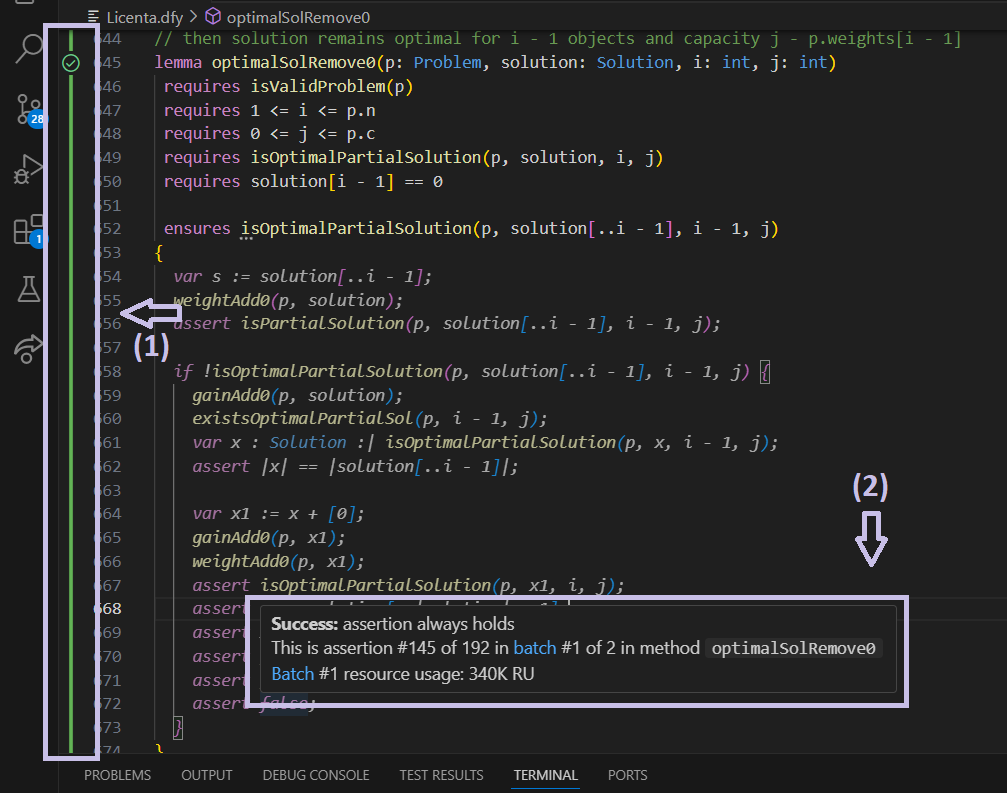
\includegraphics[width=0.6\linewidth]{images/imageVerificationSucceeded.png}
\end{figure}
 \par De exemplu, pentru lema \formatText{optimalSolRemove0} Dafny a reușit să verifice cu succes corectitudinea acesteia, iar acest lucru este evidențiat printr-o bară verticală de culoare verde pe toată lungimea declarației acesteia. În funcție de starea procesului de verificare, această bară își va schimba stilul în mod dinamic pentru a ajuta programatorul în procesul de dezvoltare al codului.
 \par De asemenea, dacă plasăm cursorul peste o instrucțiune, o fereastră pop-up apare în care putem afla informații despre stadiul verificării acesteia (săgeata 2). Acest lucru este de ajutor mai mult în cazul invarianților pentru a afla dacă verificatorul nu poate demonstra corectitudinea acestuia înainte de execuția buclei sau în timpul acesteia. \\ \par
 Pentru a rula algoritmul, avem două variante:
 \begin{itemize}
     \item click dreapta în fișierul ce se dorește a fi rulat și alegem \texttt{Dafny} $\rightarrow$ \texttt{Dafny:Run} (sau \texttt{F5})
     \item din linia de comandă se poate executa următoarea comanda: \texttt{dafny run Licenta.dfy} (mai multe opțiuni de control al verificării pot fi adăugate, precum \texttt{--allow-warnings})
 \end{itemize}
 \par
Una dintre cele mai comune provocări pe care le-am întâmpinat pe parcursul procesului de implementare a fost depășirea timpului de răspuns alocat pentru verificarea unei leme sau a unei metode, care poate apărea atunci când unele specificații nu sunt complete sau când logica demonstrației este mult prea complexă pentru verificator, dar există și cazuri în care acesta se pierde încercând să demonstreze lanțuri inutile de raționament \cite{verification_optimization}. În astfel de cazuri am avut la îndemană următoarele posibilități:
\begin{itemize}
    \item Utilizarea instrucțiunilor \texttt{assert}: acestea sunt folosite pentru a verifica valoarea de adevăr a unei expresii logice necesare în demonstrație. Cu ajutorul acestora am verificat dacă Dafny poate aproba raționamentul pe care l-am aplicat în demonstrarea postcondițiilor deoarece de foarte multe ori a fost nevoie să ghidez verificatorul spre o anumită direcție logică, dar și unele proprietăți care trebuiau să fie adevărate după apelarea unor leme pentru a continua verificarea. Un exemplu foarte bun pentru ambele cazuri este lema \formatText{gainAddTooBig}:
   \begin{Verbatim}[commandchars=\\\{\}]
\PY{k+kd}{lemma} \PY{n+nf}{gainAddTooBig}\PY{p}{(}\PY{n}{p}\PY{p}{:} \PY{n}{Problem}\PY{p}{,} \PY{n}{solution}\PY{p}{:} \PY{n}{Solution}\PY{p}{,} 
    \PY{n}{i}\PY{p}{:} \PY{k+kt}{int}\PY{p}{,} \PY{n}{j}\PY{p}{:} \PY{k+kt}{int}\PY{p}{)} 
 \PY{p}{..}\PY{p}{.}
 \PY{k}{requires} \PY{n}{isPartialSolution}\PY{p}{(}\PY{n}{p}\PY{p}{,} \PY{n}{solution}\PY{p}{,} \PY{n}{i}\PY{p}{,} \PY{n}{j}\PY{p}{)}
 \PY{k}{requires} \PY{n}{p}\PY{p}{.}\PY{n}{weights}\PY{p}{[}\PY{n}{i} \PY{o}{\PYZhy{}} \PY{l+m+mi}{1}\PY{p}{]} \PY{o}{\PYZgt{}} \PY{n}{j}
 \PY{k}{ensures} \PY{n}{solution}\PY{p}{[}\PY{n}{i} \PY{o}{\PYZhy{}} \PY{l+m+mi}{1}\PY{p}{]} \PY{o}{==} \PY{l+m+mi}{0}
 \PY{k}{ensures} \PY{n}{gain}\PY{p}{(}\PY{n}{p}\PY{p}{,} \PY{n}{solution}\PY{p}{[}\PY{p}{..}\PY{n}{i} \PY{o}{\PYZhy{}} \PY{l+m+mi}{1}\PY{p}{]}\PY{p}{)} \PY{o}{==} \PY{n}{gain}\PY{p}{(}\PY{n}{p}\PY{p}{,} \PY{n}{solution}\PY{p}{)}
 \PY{p}{\PYZob{}}
    \PY{k}{if} \PY{n}{solution}\PY{p}{[}\PY{n}{i} \PY{o}{\PYZhy{}} \PY{l+m+mi}{1}\PY{p}{]} \PY{o}{==} \PY{l+m+mi}{1} \PY{p}{\PYZob{}}
      \PY{k}{assert} \PY{n}{computeWeight}\PY{p}{(}\PY{n}{p}\PY{p}{,} \PY{n}{solution}\PY{p}{,} \PY{o}{|}\PY{n}{solution}\PY{o}{|} \PY{o}{\PYZhy{}} \PY{l+m+mi}{1}\PY{p}{)} \PY{o}{==} 
        \PY{n}{computeWeight}\PY{p}{(}\PY{n}{p}\PY{p}{,} \PY{n}{solution}\PY{p}{,} \PY{o}{|}\PY{n}{solution}\PY{p}{[}\PY{p}{..}\PY{n}{i}\PY{p}{]}\PY{o}{|} \PY{o}{\PYZhy{}} \PY{l+m+mi}{1}\PY{p}{)} \PY{o}{+} 
        \PY{n}{p}\PY{p}{.}\PY{n}{weights}\PY{p}{[}\PY{n}{i} \PY{o}{\PYZhy{}} \PY{l+m+mi}{1}\PY{p}{]}\PY{p}{;}
      \PY{k}{assert} \PY{n}{weight}\PY{p}{(}\PY{n}{p}\PY{p}{,} \PY{n}{solution}\PY{p}{)} \PY{o}{\PYZgt{}=} \PY{n}{p}\PY{p}{.}\PY{n}{weights}\PY{p}{[}\PY{n}{i} \PY{o}{\PYZhy{}} \PY{l+m+mi}{1}\PY{p}{]} \PY{o}{\PYZgt{}} \PY{n}{j}\PY{p}{;}
      \PY{k}{assert} \PY{err}{!}\PY{n}{isPartialSolution}\PY{p}{(}\PY{n}{p}\PY{p}{,} \PY{n}{solution}\PY{p}{,} \PY{n}{i}\PY{p}{,} \PY{n}{j}\PY{p}{)}\PY{p}{;}
      \PY{k}{assert} \PY{k+kc}{false}\PY{p}{;}
    \PY{p}{\PYZcb{}}
    \PY{k}{assert} \PY{n}{solution}\PY{p}{[}\PY{n}{i} \PY{o}{\PYZhy{}} \PY{l+m+mi}{1}\PY{p}{]} \PY{o}{==} \PY{l+m+mi}{0}\PY{p}{;}
    \PY{n}{computeGainAdd0}\PY{p}{(}\PY{n}{p}\PY{p}{,} \PY{n}{solution}\PY{p}{,} \PY{o}{|}\PY{n}{solution}\PY{o}{|} \PY{o}{\PYZhy{}} \PY{l+m+mi}{2}\PY{p}{)}\PY{p}{;}
    \PY{k}{assert} \PY{n}{gain}\PY{p}{(}\PY{n}{p}\PY{p}{,} \PY{n}{solution}\PY{p}{[}\PY{p}{..}\PY{n}{i} \PY{o}{\PYZhy{}} \PY{l+m+mi}{1}\PY{p}{]}\PY{p}{)} \PY{o}{==} \PY{n}{gain}\PY{p}{(}\PY{n}{p}\PY{p}{,} \PY{n}{solution}\PY{p}{)}\PY{p}{;}
\PY{p}{\PYZcb{}}
\end{Verbatim}
    unde \texttt{assert-urile} din instrucțiunea \textit{if} urmăresc să ajungem la o contradicție prin faptul că soluția nu are cum să fie parțială dacă greutatea obiectului depășește capacitatea $j$, propoziție care este falsă deoarece avem o precondiție care asigură exact acest lucru, iar instrucțiunea 
    \begin{Verbatim}[commandchars=\\\{\}]
\PY{k}{assert} \PY{n}{gain}\PY{p}{(}\PY{n}{p}\PY{p}{,} \PY{n}{solution}\PY{p}{[}\PY{p}{..}\PY{n}{i} \PY{o}{\PYZhy{}} \PY{l+m+mi}{1}\PY{p}{]}\PY{p}{)} \PY{o}{==} \PY{n}{gain}\PY{p}{(}\PY{n}{p}\PY{p}{,} \PY{n}{solution}\PY{p}{)}\PY{p}{;}
\end{Verbatim}
    se asigură că după apelarea lemei computeGainAdd0 verificatorul știe că profitul unei soluții rămâne neschimbat dacă eliminăm ultimul element de 0 din soluție. \par
    \hspace{2mm} De asemenea, folosind structura \texttt{assert ... by} putem reduce sarcina verificatorului deoarece pașii din acest bloc de instrucțiuni sunt "uitați" după verificarea condiției din assert:
    \begin{Verbatim}[commandchars=\\\{\}]
\PY{k}{assert} \PY{n}{gain}\PY{p}{(}\PY{n}{p}\PY{p}{,} \PY{n}{x}\PY{p}{[}\PY{p}{..}\PY{n}{i} \PY{o}{\PYZhy{}} \PY{l+m+mi}{1}\PY{p}{]}\PY{p}{)} \PY{o}{==} \PY{n}{gain}\PY{p}{(}\PY{n}{p}\PY{p}{,} \PY{n}{solution1}\PY{p}{)} \PY{n}{by}
\PY{p}{\PYZob{}}
  \PY{n}{optimalSolRemove1}\PY{p}{(}\PY{n}{p}\PY{p}{,} \PY{n}{x}\PY{p}{,} \PY{n}{i}\PY{p}{,} \PY{n}{j}\PY{p}{)}\PY{p}{;}
  \PY{k}{assert} \PY{n}{isOptimalPartialSolution}\PY{p}{(}\PY{n}{p}\PY{p}{,} \PY{n}{x}\PY{p}{[}\PY{p}{..}\PY{n}{i} \PY{o}{\PYZhy{}} \PY{l+m+mi}{1}\PY{p}{]}\PY{p}{,} 
    \PY{n}{i} \PY{o}{\PYZhy{}} \PY{l+m+mi}{1}\PY{p}{,} \PY{n}{j} \PY{o}{\PYZhy{}} \PY{n}{p}\PY{p}{.}\PY{n}{weights}\PY{p}{[}\PY{n}{i} \PY{o}{\PYZhy{}} \PY{l+m+mi}{1}\PY{p}{]}\PY{p}{)}\PY{p}{;}
\PY{p}{\PYZcb{}} 
\end{Verbatim}
    \item Utilizarea instrucțiunii \texttt{assume}: această instrucțiune este foarte utilă pentru a determina la ce linie întâlnește Dafny probleme. O instrucțiune \texttt{assume} tratează condiția ca fiind adevarată, de aceea de multe ori am folosit-o pentru a afla de ce informații în plus are nevoie verificatorul sau pentru a putea continua următorii pași ai demonstrației. De exemplu, mi-a fost de ajutor în cazul lemelor în care presupun că există o soluție mai bună decât cea pentru care vreau să demonstrez că este optimă, întrucât am putut continua implementarea acestora, după care am revenit să formulez o lemă specială pentru a demonstra existența unor astfel de soluții. \par
    \hspace{2mm} O altă utilizare a instrucțiunii assume a fost \texttt{assume false} care oprește verificarea pentru condițiile ce urmează după aceasta și îi indică verificatorului să nu mai încerce demonstrarea acestora și să accepte orice afirmație ulterioară ca fiind adevărată. Aceasta instrucțiune a fost foarte folositoare pentru a identifica ce assert-uri nu reușea Dafny să demonstreze pentru lemele mai complexe, mai ales în cazul instrucțiunilor \textit{if} din cadrul lemelor unde pe fiecare ramură aveam o logică diferită și ambele puteau cauza probleme de logică.
    \item \formatText{Modularizare}: în leme precum \formatText{optimalSolAdd1} și \formatText{optimalSolAdd0}, unde deși demonstrația era corectă și fiecare caz (când ultimul element este fie 0, fie 1) se verifica cu succes separat, dacă ambele erau tratate în cadrul aceleași leme obțineam acest timeout deoarece demonstrația era destul de complexă pentru Dafny. Soluția a fost astfel să tratez unul dintre cele două cazuri posibile într-o lemă separată.
\end{itemize}

\end{sloppypar}
    
    \chapter*{Concluzii} 
\addcontentsline{toc}{chapter}{Concluzii}

-
    \bibliography{chapters/references} 
    \bibliographystyle{ieeetr}

    \subsection*{Codul sursă} 
\begin{scriptsize}
\begin{Verbatim}[commandchars=\\\{\}]
\PY{k+kd}{datatype} \PY{n+nc}{Problem} \PY{o}{=} \PY{n}{Problem}\PY{p}{(}\PY{n}{n}\PY{p}{:} \PY{k+kt}{int}\PY{p}{,} \PY{n}{c}\PY{p}{:} \PY{k+kt}{int}\PY{p}{,} \PY{n}{gains}\PY{p}{:} \PY{k+kt}{seq}\PY{o}{\PYZlt{}}\PY{k+kt}{int}\PY{o}{\PYZgt{}}\PY{p}{,} \PY{n}{weights}\PY{p}{:} \PY{k+kt}{seq}\PY{o}{\PYZlt{}}\PY{k+kt}{int}\PY{o}{\PYZgt{}}\PY{p}{)}

\PY{n}{type} \PY{n}{Solution} \PY{o}{=} \PY{k+kt}{seq}\PY{o}{\PYZlt{}}\PY{k+kt}{int}\PY{o}{\PYZgt{}} 

\PY{k+kd}{function} \PY{n+nf}{gain}\PY{p}{(}\PY{n}{p}\PY{p}{:} \PY{n}{Problem}\PY{p}{,} \PY{n}{solution}\PY{p}{:} \PY{n}{Solution}\PY{p}{)}\PY{p}{:} \PY{k+kt}{int}
  \PY{k}{requires} \PY{n}{isValidProblem}\PY{p}{(}\PY{n}{p}\PY{p}{)}
  \PY{k}{requires} \PY{n}{hasAllowedValues}\PY{p}{(}\PY{n}{solution}\PY{p}{)}
  \PY{k}{requires} \PY{l+m+mi}{0} \PY{o}{\PYZlt{}=} \PY{o}{|}\PY{n}{solution}\PY{o}{|} \PY{o}{\PYZlt{}=} \PY{n}{p}\PY{p}{.}\PY{n}{n}
\PY{p}{\PYZob{}}
  \PY{k}{if} \PY{o}{|}\PY{n}{solution}\PY{o}{|} \PY{o}{==} \PY{l+m+mi}{0} \PY{k}{then} \PY{l+m+mi}{0} \PY{k}{else} \PY{n}{computeGain}\PY{p}{(}\PY{n}{p}\PY{p}{,} \PY{n}{solution}\PY{p}{,} \PY{o}{|}\PY{n}{solution}\PY{o}{|} \PY{o}{\PYZhy{}} \PY{l+m+mi}{1}\PY{p}{)}
\PY{p}{\PYZcb{}}

\PY{k+kd}{function} \PY{n+nf}{computeGain}\PY{p}{(}\PY{n}{p}\PY{p}{:} \PY{n}{Problem}\PY{p}{,} \PY{n}{solution}\PY{p}{:} \PY{n}{Solution}\PY{p}{,} \PY{n}{i}\PY{p}{:} \PY{k+kt}{int}\PY{p}{)} \PY{p}{:} \PY{k+kt}{int}
  \PY{k}{requires} \PY{n}{isValidProblem}\PY{p}{(}\PY{n}{p}\PY{p}{)}
  \PY{k}{requires} \PY{l+m+mi}{0} \PY{o}{\PYZlt{}=} \PY{n}{i} \PY{o}{\PYZlt{}} \PY{o}{|}\PY{n}{solution}\PY{o}{|}
  \PY{k}{requires} \PY{l+m+mi}{0} \PY{o}{\PYZlt{}=} \PY{n}{i} \PY{o}{\PYZlt{}} \PY{o}{|}\PY{n}{p}\PY{p}{.}\PY{n}{gains}\PY{o}{|}
  \PY{k}{requires} \PY{n}{hasAllowedValues}\PY{p}{(}\PY{n}{solution}\PY{p}{)}
  \PY{k}{requires} \PY{l+m+mi}{0} \PY{o}{\PYZlt{}=} \PY{o}{|}\PY{n}{solution}\PY{o}{|} \PY{o}{\PYZlt{}=} \PY{o}{|}\PY{n}{p}\PY{p}{.}\PY{n}{gains}\PY{o}{|}
  \PY{k}{ensures} \PY{n}{computeGain}\PY{p}{(}\PY{n}{p}\PY{p}{,} \PY{n}{solution}\PY{p}{,} \PY{n}{i}\PY{p}{)} \PY{o}{\PYZgt{}=} \PY{l+m+mi}{0}
\PY{p}{\PYZob{}}
  \PY{k}{if} \PY{n}{i} \PY{o}{==} \PY{l+m+mi}{0} \PY{k}{then} \PY{n}{solution}\PY{p}{[}\PY{l+m+mi}{0}\PY{p}{]} \PY{o}{*} \PY{n}{p}\PY{p}{.}\PY{n}{gains}\PY{p}{[}\PY{l+m+mi}{0}\PY{p}{]} \PY{k}{else} 
        \PY{n}{solution}\PY{p}{[}\PY{n}{i}\PY{p}{]} \PY{o}{*} \PY{n}{p}\PY{p}{.}\PY{n}{gains}\PY{p}{[}\PY{n}{i}\PY{p}{]} \PY{o}{+} \PY{n}{computeGain}\PY{p}{(}\PY{n}{p}\PY{p}{,} \PY{n}{solution}\PY{p}{,} \PY{n}{i} \PY{o}{\PYZhy{}} \PY{l+m+mi}{1}\PY{p}{)}
\PY{p}{\PYZcb{}}

\PY{k+kd}{function} \PY{n+nf}{weight}\PY{p}{(}\PY{n}{p}\PY{p}{:} \PY{n}{Problem}\PY{p}{,} \PY{n}{solution}\PY{p}{:} \PY{n}{Solution}\PY{p}{)}\PY{p}{:} \PY{k+kt}{int}
  \PY{k}{requires} \PY{n}{isValidProblem}\PY{p}{(}\PY{n}{p}\PY{p}{)}
  \PY{k}{requires} \PY{n}{hasAllowedValues}\PY{p}{(}\PY{n}{solution}\PY{p}{)}
  \PY{k}{requires} \PY{l+m+mi}{0} \PY{o}{\PYZlt{}=} \PY{o}{|}\PY{n}{solution}\PY{o}{|} \PY{o}{\PYZlt{}=} \PY{n}{p}\PY{p}{.}\PY{n}{n}
\PY{p}{\PYZob{}}
  \PY{k}{if} \PY{o}{|}\PY{n}{solution}\PY{o}{|} \PY{o}{==} \PY{l+m+mi}{0} \PY{k}{then} \PY{l+m+mi}{0} \PY{k}{else} \PY{n}{computeWeight}\PY{p}{(}\PY{n}{p}\PY{p}{,} \PY{n}{solution}\PY{p}{,} \PY{o}{|}\PY{n}{solution}\PY{o}{|} \PY{o}{\PYZhy{}} \PY{l+m+mi}{1}\PY{p}{)}
\PY{p}{\PYZcb{}}

\PY{k+kd}{function} \PY{n+nf}{computeWeight}\PY{p}{(}\PY{n}{p}\PY{p}{:} \PY{n}{Problem}\PY{p}{,} \PY{n}{solution}\PY{p}{:} \PY{n}{Solution}\PY{p}{,} \PY{n}{i}\PY{p}{:} \PY{k+kt}{int}\PY{p}{)} \PY{p}{:} \PY{k+kt}{int}
  \PY{k}{requires} \PY{k}{forall} \PY{n}{i} \PY{p}{::} \PY{l+m+mi}{0} \PY{o}{\PYZlt{}=} \PY{n}{i} \PY{o}{\PYZlt{}} \PY{o}{|}\PY{n}{p}\PY{p}{.}\PY{n}{weights}\PY{o}{|} \PY{o}{==}\PY{o}{\PYZgt{}} \PY{n}{p}\PY{p}{.}\PY{n}{weights}\PY{p}{[}\PY{n}{i}\PY{p}{]} \PY{o}{\PYZgt{}} \PY{l+m+mi}{0} 
  \PY{k}{requires} \PY{l+m+mi}{0} \PY{o}{\PYZlt{}=} \PY{n}{i} \PY{o}{\PYZlt{}} \PY{o}{|}\PY{n}{solution}\PY{o}{|}
  \PY{k}{requires} \PY{l+m+mi}{0} \PY{o}{\PYZlt{}=} \PY{n}{i} \PY{o}{\PYZlt{}} \PY{o}{|}\PY{n}{p}\PY{p}{.}\PY{n}{weights}\PY{o}{|}
  \PY{k}{requires} \PY{n}{hasAllowedValues}\PY{p}{(}\PY{n}{solution}\PY{p}{)}
  \PY{k}{requires} \PY{l+m+mi}{0} \PY{o}{\PYZlt{}=} \PY{o}{|}\PY{n}{solution}\PY{o}{|} \PY{o}{\PYZlt{}=} \PY{o}{|}\PY{n}{p}\PY{p}{.}\PY{n}{weights}\PY{o}{|}
  \PY{k}{ensures} \PY{n}{computeWeight}\PY{p}{(}\PY{n}{p}\PY{p}{,} \PY{n}{solution}\PY{p}{,} \PY{n}{i}\PY{p}{)} \PY{o}{\PYZgt{}=} \PY{l+m+mi}{0}
\PY{p}{\PYZob{}}
  \PY{k}{if} \PY{n}{i} \PY{o}{==} \PY{l+m+mi}{0} \PY{k}{then} \PY{n}{solution}\PY{p}{[}\PY{l+m+mi}{0}\PY{p}{]} \PY{o}{*} \PY{n}{p}\PY{p}{.}\PY{n}{weights}\PY{p}{[}\PY{l+m+mi}{0}\PY{p}{]} \PY{k}{else} 
        \PY{n}{solution}\PY{p}{[}\PY{n}{i}\PY{p}{]} \PY{o}{*} \PY{n}{p}\PY{p}{.}\PY{n}{weights}\PY{p}{[}\PY{n}{i}\PY{p}{]} \PY{o}{+} \PY{n}{computeWeight}\PY{p}{(}\PY{n}{p}\PY{p}{,} \PY{n}{solution}\PY{p}{,} \PY{n}{i} \PY{o}{\PYZhy{}} \PY{l+m+mi}{1}\PY{p}{)}
\PY{p}{\PYZcb{}}

\PY{k+kd}{function} \PY{n+nf}{sumAllGains}\PY{p}{(}\PY{n}{p}\PY{p}{:} \PY{n}{Problem}\PY{p}{,} \PY{n}{i}\PY{p}{:} \PY{k+kt}{int}\PY{p}{)} \PY{p}{:} \PY{k+kt}{int}
 \PY{k}{requires} \PY{n}{isValidProblem}\PY{p}{(}\PY{n}{p}\PY{p}{)}
 \PY{k}{requires} \PY{l+m+mi}{1} \PY{o}{\PYZlt{}=} \PY{n}{i} \PY{o}{\PYZlt{}=} \PY{n}{p}\PY{p}{.}\PY{n}{n}
 \PY{k}{ensures} \PY{n}{sumAllGains}\PY{p}{(}\PY{n}{p}\PY{p}{,} \PY{n}{i}\PY{p}{)} \PY{o}{\PYZgt{}=} \PY{l+m+mi}{0}
\PY{p}{\PYZob{}}
  \PY{k}{if} \PY{p}{(}\PY{n}{i} \PY{o}{==} \PY{l+m+mi}{1}\PY{p}{)} \PY{k}{then} \PY{n}{p}\PY{p}{.}\PY{n}{gains}\PY{p}{[}\PY{l+m+mi}{0}\PY{p}{]} \PY{k}{else} \PY{n}{p}\PY{p}{.}\PY{n}{gains}\PY{p}{[}\PY{n}{i} \PY{o}{\PYZhy{}} \PY{l+m+mi}{1}\PY{p}{]} \PY{o}{+} \PY{n}{sumAllGains}\PY{p}{(}\PY{n}{p}\PY{p}{,} \PY{n}{i} \PY{o}{\PYZhy{}}\PY{l+m+mi}{1}\PY{p}{)}
\PY{p}{\PYZcb{}}

\PY{k+kd}{predicate} \PY{n+nf}{hasPositiveValues}\PY{p}{(}\PY{n}{arr}\PY{p}{:} \PY{k+kt}{seq}\PY{o}{\PYZlt{}}\PY{k+kt}{int}\PY{o}{\PYZgt{}}\PY{p}{)}
\PY{p}{\PYZob{}}
  \PY{k}{forall} \PY{n}{i} \PY{p}{::} \PY{l+m+mi}{0} \PY{o}{\PYZlt{}=} \PY{n}{i} \PY{o}{\PYZlt{}} \PY{o}{|}\PY{n}{arr}\PY{o}{|} \PY{o}{==}\PY{o}{\PYZgt{}} \PY{n}{arr}\PY{p}{[}\PY{n}{i}\PY{p}{]} \PY{o}{\PYZgt{}} \PY{l+m+mi}{0}
\PY{p}{\PYZcb{}}

\PY{k+kd}{predicate} \PY{n+nf}{hasAllowedValues}\PY{p}{(}\PY{n}{solution}\PY{p}{:} \PY{n}{Solution}\PY{p}{)}
\PY{p}{\PYZob{}}
  \PY{k}{forall} \PY{n}{k} \PY{p}{::} \PY{l+m+mi}{0} \PY{o}{\PYZlt{}=} \PY{n}{k} \PY{o}{\PYZlt{}} \PY{o}{|}\PY{n}{solution}\PY{o}{|} \PY{o}{==}\PY{o}{\PYZgt{}} \PY{n}{solution}\PY{p}{[}\PY{n}{k}\PY{p}{]} \PY{o}{==} \PY{l+m+mi}{0} \PY{o}{|}\PY{o}{|} \PY{n}{solution}\PY{p}{[}\PY{n}{k}\PY{p}{]} \PY{o}{==} \PY{l+m+mi}{1}
\PY{p}{\PYZcb{}}

\PY{k+kd}{predicate} \PY{n+nf}{isValidProblem}\PY{p}{(}\PY{n}{p}\PY{p}{:} \PY{n}{Problem}\PY{p}{)}
\PY{p}{\PYZob{}}
  \PY{o}{|}\PY{n}{p}\PY{p}{.}\PY{n}{gains}\PY{o}{|} \PY{o}{==} \PY{o}{|}\PY{n}{p}\PY{p}{.}\PY{n}{weights}\PY{o}{|} \PY{o}{==} \PY{n}{p}\PY{p}{.}\PY{n}{n} \PY{o}{\PYZam{}\PYZam{}} 
  \PY{n}{p}\PY{p}{.}\PY{n}{n} \PY{o}{\PYZgt{}} \PY{l+m+mi}{0} \PY{o}{\PYZam{}\PYZam{}} \PY{n}{p}\PY{p}{.}\PY{n}{c} \PY{o}{\PYZgt{}=} \PY{l+m+mi}{0} \PY{o}{\PYZam{}\PYZam{}} 
  \PY{n}{hasPositiveValues}\PY{p}{(}\PY{n}{p}\PY{p}{.}\PY{n}{gains}\PY{p}{)} \PY{o}{\PYZam{}\PYZam{}} \PY{n}{hasPositiveValues}\PY{p}{(}\PY{n}{p}\PY{p}{.}\PY{n}{weights}\PY{p}{)} 
\PY{p}{\PYZcb{}}

\PY{k+kd}{predicate} \PY{n+nf}{isValidPartialSolution}\PY{p}{(}\PY{n}{p}\PY{p}{:} \PY{n}{Problem}\PY{p}{,} \PY{n}{solution}\PY{p}{:} \PY{n}{Solution}\PY{p}{)}
  \PY{k}{requires} \PY{n}{isValidProblem}\PY{p}{(}\PY{n}{p}\PY{p}{)}
\PY{p}{\PYZob{}}
  \PY{n}{hasAllowedValues}\PY{p}{(}\PY{n}{solution}\PY{p}{)} \PY{o}{\PYZam{}\PYZam{}} \PY{o}{|}\PY{n}{solution}\PY{o}{|} \PY{o}{\PYZlt{}=} \PY{n}{p}\PY{p}{.}\PY{n}{n}
\PY{p}{\PYZcb{}}

\PY{k+kd}{predicate} \PY{n+nf}{isPartialSolution}\PY{p}{(}\PY{n}{p}\PY{p}{:} \PY{n}{Problem}\PY{p}{,} \PY{n}{solution}\PY{p}{:} \PY{n}{Solution}\PY{p}{,} \PY{n}{i}\PY{p}{:} \PY{k+kt}{int}\PY{p}{,} \PY{n}{j}\PY{p}{:} \PY{k+kt}{int}\PY{p}{)}
  \PY{k}{requires} \PY{n}{isValidProblem}\PY{p}{(}\PY{n}{p}\PY{p}{)}
  \PY{k}{requires} \PY{l+m+mi}{0} \PY{o}{\PYZlt{}=} \PY{n}{i} \PY{o}{\PYZlt{}=} \PY{n}{p}\PY{p}{.}\PY{n}{n}
  \PY{k}{requires} \PY{l+m+mi}{0} \PY{o}{\PYZlt{}=} \PY{n}{j} \PY{o}{\PYZlt{}=} \PY{n}{p}\PY{p}{.}\PY{n}{c}
\PY{p}{\PYZob{}}
  \PY{n}{isValidPartialSolution}\PY{p}{(}\PY{n}{p}\PY{p}{,} \PY{n}{solution}\PY{p}{)} \PY{o}{\PYZam{}\PYZam{}} \PY{o}{|}\PY{n}{solution}\PY{o}{|} \PY{o}{==} \PY{n}{i} \PY{o}{\PYZam{}\PYZam{}}
  \PY{n}{weight}\PY{p}{(}\PY{n}{p}\PY{p}{,} \PY{n}{solution}\PY{p}{)} \PY{o}{\PYZlt{}=} \PY{n}{j}
\PY{p}{\PYZcb{}}

\PY{k+kd}{predicate} \PY{n+nf}{isSolution}\PY{p}{(}\PY{n}{p}\PY{p}{:} \PY{n}{Problem}\PY{p}{,} \PY{n}{solution}\PY{p}{:} \PY{n}{Solution}\PY{p}{)}
  \PY{k}{requires} \PY{n}{isValidProblem}\PY{p}{(}\PY{n}{p}\PY{p}{)}
\PY{p}{\PYZob{}}
  \PY{n}{isValidPartialSolution}\PY{p}{(}\PY{n}{p}\PY{p}{,} \PY{n}{solution}\PY{p}{)} \PY{o}{\PYZam{}\PYZam{}} \PY{o}{|}\PY{n}{solution}\PY{o}{|} \PY{o}{==} \PY{n}{p}\PY{p}{.}\PY{n}{n} \PY{o}{\PYZam{}\PYZam{}}
  \PY{n}{weight}\PY{p}{(}\PY{n}{p}\PY{p}{,} \PY{n}{solution}\PY{p}{)} \PY{o}{\PYZlt{}=} \PY{n}{p}\PY{p}{.}\PY{n}{c}
\PY{p}{\PYZcb{}}

\PY{k+kd}{ghost} \PY{k+kd}{predicate} \PY{n+nf}{isOptimalPartialSolution}\PY{p}{(}\PY{n}{p}\PY{p}{:} \PY{n}{Problem}\PY{p}{,} \PY{n}{solution}\PY{p}{:} \PY{n}{Solution}\PY{p}{,} \PY{n}{i}\PY{p}{:} \PY{k+kt}{int}\PY{p}{,} \PY{n}{j}\PY{p}{:} \PY{k+kt}{int}\PY{p}{)}
  \PY{k}{requires} \PY{n}{isValidProblem}\PY{p}{(}\PY{n}{p}\PY{p}{)}
  \PY{k}{requires} \PY{l+m+mi}{0} \PY{o}{\PYZlt{}=} \PY{n}{i} \PY{o}{\PYZlt{}=} \PY{n}{p}\PY{p}{.}\PY{n}{n}
  \PY{k}{requires} \PY{l+m+mi}{0} \PY{o}{\PYZlt{}=} \PY{n}{j} \PY{o}{\PYZlt{}=} \PY{n}{p}\PY{p}{.}\PY{n}{c}
\PY{p}{\PYZob{}}
  \PY{n}{isPartialSolution}\PY{p}{(}\PY{n}{p}\PY{p}{,} \PY{n}{solution}\PY{p}{,} \PY{n}{i}\PY{p}{,} \PY{n}{j}\PY{p}{)} \PY{o}{\PYZam{}\PYZam{}}
  \PY{k}{forall} \PY{n}{s}\PY{p}{:} \PY{n}{Solution} \PY{p}{::} \PY{p}{(}\PY{n}{isPartialSolution}\PY{p}{(}\PY{n}{p}\PY{p}{,} \PY{n}{s}\PY{p}{,} \PY{n}{i}\PY{p}{,} \PY{n}{j}\PY{p}{)} \PY{o}{\PYZam{}\PYZam{}} \PY{o}{|}\PY{n}{s}\PY{o}{|} \PY{o}{==} \PY{o}{|}\PY{n}{solution}\PY{o}{|} 
      \PY{o}{==}\PY{o}{\PYZgt{}} \PY{n}{gain}\PY{p}{(}\PY{n}{p}\PY{p}{,} \PY{n}{solution}\PY{p}{)} \PY{o}{\PYZgt{}=} \PY{n}{gain}\PY{p}{(}\PY{n}{p}\PY{p}{,} \PY{n}{s}\PY{p}{)}\PY{p}{)}
\PY{p}{\PYZcb{}}

\PY{k+kd}{ghost} \PY{k+kd}{predicate} \PY{n+nf}{isOptimalSolution}\PY{p}{(}\PY{n}{p}\PY{p}{:} \PY{n}{Problem}\PY{p}{,} \PY{n}{solution}\PY{p}{:} \PY{n}{Solution}\PY{p}{)}
  \PY{k}{requires} \PY{n}{isValidProblem}\PY{p}{(}\PY{n}{p}\PY{p}{)}
  \PY{k}{requires} \PY{n}{isValidPartialSolution}\PY{p}{(}\PY{n}{p}\PY{p}{,} \PY{n}{solution}\PY{p}{)}
\PY{p}{\PYZob{}}
  \PY{n}{isOptimalPartialSolution}\PY{p}{(}\PY{n}{p}\PY{p}{,} \PY{n}{solution}\PY{p}{,} \PY{n}{p}\PY{p}{.}\PY{n}{n}\PY{p}{,} \PY{n}{p}\PY{p}{.}\PY{n}{c}\PY{p}{)} \PY{o}{\PYZam{}\PYZam{}}
  \PY{k}{forall} \PY{n}{s}\PY{p}{:} \PY{n}{Solution} \PY{p}{::} \PY{p}{(}\PY{p}{(}\PY{p}{(}\PY{n}{isOptimalPartialSolution}\PY{p}{(}\PY{n}{p}\PY{p}{,} \PY{n}{s}\PY{p}{,} \PY{n}{p}\PY{p}{.}\PY{n}{n}\PY{p}{,} \PY{n}{p}\PY{p}{.}\PY{n}{c}\PY{p}{)}\PY{p}{)} \PY{o}{==}\PY{o}{\PYZgt{}} 
  \PY{n}{gain}\PY{p}{(}\PY{n}{p}\PY{p}{,} \PY{n}{solution}\PY{p}{)} \PY{o}{\PYZgt{}=} \PY{n}{gain}\PY{p}{(}\PY{n}{p}\PY{p}{,} \PY{n}{s}\PY{p}{)}\PY{p}{)}\PY{p}{)}
\PY{p}{\PYZcb{}}

\PY{k+kd}{predicate} \PY{n+nf}{isValidSubproblem}\PY{p}{(}\PY{n}{p}\PY{p}{:} \PY{n}{Problem}\PY{p}{,} \PY{n}{i}\PY{p}{:} \PY{k+kt}{int}\PY{p}{,} \PY{n}{j}\PY{p}{:} \PY{k+kt}{int}\PY{p}{)}
\PY{p}{\PYZob{}}
  \PY{n}{isValidProblem}\PY{p}{(}\PY{n}{p}\PY{p}{)} \PY{o}{\PYZam{}\PYZam{}} 
  \PY{l+m+mi}{1} \PY{o}{\PYZlt{}=} \PY{n}{i} \PY{o}{\PYZlt{}=} \PY{n}{p}\PY{p}{.}\PY{n}{n} \PY{o}{\PYZam{}\PYZam{}} 
  \PY{l+m+mi}{1} \PY{o}{\PYZlt{}=} \PY{n}{j} \PY{o}{\PYZlt{}=} \PY{n}{p}\PY{p}{.}\PY{n}{c} 
\PY{p}{\PYZcb{}}

\PY{k+kd}{ghost} \PY{k+kd}{predicate} \PY{n+nf}{areValidSolutions}\PY{p}{(}\PY{n}{p}\PY{p}{:} \PY{n}{Problem}\PY{p}{,} \PY{n}{profits}\PY{p}{:} \PY{k+kt}{seq}\PY{o}{\PYZlt{}}\PY{k+kt}{seq}\PY{o}{\PYZlt{}}\PY{k+kt}{int}\PY{o}{\PYZgt{}}\PY{o}{\PYZgt{}}\PY{p}{,} \PY{n}{solutions}\PY{p}{:} \PY{k+kt}{seq}\PY{o}{\PYZlt{}}\PY{k+kt}{seq}\PY{o}{\PYZlt{}}\PY{k+kt}{seq}\PY{o}{\PYZlt{}}\PY{k+kt}{int}\PY{o}{\PYZgt{}}\PY{o}{\PYZgt{}}\PY{o}{\PYZgt{}}\PY{p}{,} 
  \PY{n}{i}\PY{p}{:} \PY{k+kt}{int}\PY{p}{)} 
  \PY{k}{requires} \PY{n}{isValidSubproblem}\PY{p}{(}\PY{n}{p}\PY{p}{,} \PY{n}{i}\PY{p}{,} \PY{n}{p}\PY{p}{.}\PY{n}{c}\PY{p}{)}
\PY{p}{\PYZob{}} 
  \PY{n}{i} \PY{o}{==} \PY{o}{|}\PY{n}{profits}\PY{o}{|} \PY{o}{==} \PY{o}{|}\PY{n}{solutions}\PY{o}{|} \PY{o}{\PYZam{}\PYZam{}}
  \PY{p}{(}\PY{k}{forall} \PY{n}{k} \PY{p}{::} \PY{l+m+mi}{0} \PY{o}{\PYZlt{}=} \PY{n}{k} \PY{o}{\PYZlt{}} \PY{n}{i} \PY{o}{==}\PY{o}{\PYZgt{}} \PY{o}{|}\PY{n}{profits}\PY{p}{[}\PY{n}{k}\PY{p}{]}\PY{o}{|} \PY{o}{==} \PY{o}{|}\PY{n}{solutions}\PY{p}{[}\PY{n}{k}\PY{p}{]}\PY{o}{|} \PY{o}{==} \PY{n}{p}\PY{p}{.}\PY{n}{c} \PY{o}{+} \PY{l+m+mi}{1}\PY{p}{)} \PY{o}{\PYZam{}\PYZam{}} 
  \PY{p}{(}\PY{k}{forall} \PY{n}{k} \PY{p}{::} \PY{l+m+mi}{0} \PY{o}{\PYZlt{}=} \PY{n}{k} \PY{o}{\PYZlt{}} \PY{o}{|}\PY{n}{solutions}\PY{o}{|} \PY{o}{==}\PY{o}{\PYZgt{}} \PY{k}{forall} \PY{n}{q} \PY{p}{::} \PY{l+m+mi}{0} \PY{o}{\PYZlt{}=} \PY{n}{q} \PY{o}{\PYZlt{}} \PY{o}{|}\PY{n}{solutions}\PY{p}{[}\PY{n}{k}\PY{p}{]}\PY{o}{|} \PY{o}{==}\PY{o}{\PYZgt{}} 
                    \PY{n}{isOptimalPartialSolution}\PY{p}{(}\PY{n}{p}\PY{p}{,} \PY{n}{solutions}\PY{p}{[}\PY{n}{k}\PY{p}{]}\PY{p}{[}\PY{n}{q}\PY{p}{]}\PY{p}{,} \PY{n}{k}\PY{p}{,} \PY{n}{q}\PY{p}{)}\PY{p}{)} \PY{o}{\PYZam{}\PYZam{}} 
  \PY{p}{(}\PY{k}{forall} \PY{n}{k} \PY{p}{::} \PY{l+m+mi}{0} \PY{o}{\PYZlt{}=} \PY{n}{k} \PY{o}{\PYZlt{}} \PY{o}{|}\PY{n}{solutions}\PY{o}{|} \PY{o}{==}\PY{o}{\PYZgt{}} \PY{k}{forall} \PY{n}{q} \PY{p}{::} \PY{l+m+mi}{0} \PY{o}{\PYZlt{}=} \PY{n}{q} \PY{o}{\PYZlt{}} \PY{o}{|}\PY{n}{solutions}\PY{p}{[}\PY{n}{k}\PY{p}{]}\PY{o}{|} \PY{o}{==}\PY{o}{\PYZgt{}} 
                \PY{n}{gain}\PY{p}{(}\PY{n}{p}\PY{p}{,} \PY{n}{solutions}\PY{p}{[}\PY{n}{k}\PY{p}{]}\PY{p}{[}\PY{n}{q}\PY{p}{]}\PY{p}{)} \PY{o}{==} \PY{n}{profits}\PY{p}{[}\PY{n}{k}\PY{p}{]}\PY{p}{[}\PY{n}{q}\PY{p}{]}\PY{p}{)}
\PY{p}{\PYZcb{}}

\PY{k+kd}{ghost} \PY{k+kd}{predicate} \PY{n+nf}{areValidPartialSolutions}\PY{p}{(}\PY{n}{p}\PY{p}{:} \PY{n}{Problem}\PY{p}{,} \PY{n}{profits}\PY{p}{:} \PY{k+kt}{seq}\PY{o}{\PYZlt{}}\PY{k+kt}{seq}\PY{o}{\PYZlt{}}\PY{k+kt}{int}\PY{o}{\PYZgt{}}\PY{o}{\PYZgt{}}\PY{p}{,} \PY{n}{solutions}\PY{p}{:} 
        \PY{k+kt}{seq}\PY{o}{\PYZlt{}}\PY{k+kt}{seq}\PY{o}{\PYZlt{}}\PY{k+kt}{seq}\PY{o}{\PYZlt{}}\PY{k+kt}{int}\PY{o}{\PYZgt{}}\PY{o}{\PYZgt{}}\PY{o}{\PYZgt{}}\PY{p}{,} \PY{n}{partialProfits}\PY{p}{:} \PY{k+kt}{seq}\PY{o}{\PYZlt{}}\PY{k+kt}{int}\PY{o}{\PYZgt{}}\PY{p}{,} \PY{n}{partialSolutions}\PY{p}{:} \PY{k+kt}{seq}\PY{o}{\PYZlt{}}\PY{k+kt}{seq}\PY{o}{\PYZlt{}}\PY{k+kt}{int}\PY{o}{\PYZgt{}}\PY{o}{\PYZgt{}}\PY{p}{,} \PY{n}{i}\PY{p}{:} \PY{k+kt}{int}\PY{p}{,} \PY{n}{j}\PY{p}{:} \PY{k+kt}{int}\PY{p}{)}               
  \PY{k}{requires} \PY{n}{isValidSubproblem}\PY{p}{(}\PY{n}{p}\PY{p}{,} \PY{n}{i}\PY{p}{,} \PY{n}{j}\PY{p}{)}
\PY{p}{\PYZob{}}
  \PY{o}{|}\PY{n}{partialSolutions}\PY{o}{|} \PY{o}{==} \PY{o}{|}\PY{n}{partialProfits}\PY{o}{|} \PY{o}{==} \PY{n}{j} \PY{o}{\PYZam{}\PYZam{}} 
  \PY{p}{(}\PY{k}{forall} \PY{n}{k} \PY{p}{::} \PY{l+m+mi}{0} \PY{o}{\PYZlt{}=} \PY{n}{k} \PY{o}{\PYZlt{}} \PY{o}{|}\PY{n}{partialSolutions}\PY{o}{|} \PY{o}{==}\PY{o}{\PYZgt{}} \PY{n}{isOptimalPartialSolution}\PY{p}{(}\PY{n}{p}\PY{p}{,} \PY{n}{partialSolutions}\PY{p}{[}\PY{n}{k}\PY{p}{]}\PY{p}{,} \PY{n}{i}\PY{p}{,} \PY{n}{k}\PY{p}{)}\PY{p}{)} \PY{o}{\PYZam{}\PYZam{}} 
  \PY{p}{(}\PY{k}{forall} \PY{n}{k} \PY{p}{::} \PY{l+m+mi}{0} \PY{o}{\PYZlt{}=} \PY{n}{k} \PY{o}{\PYZlt{}} \PY{o}{|}\PY{n}{partialSolutions}\PY{o}{|} \PY{o}{==}\PY{o}{\PYZgt{}} \PY{n}{gain}\PY{p}{(}\PY{n}{p}\PY{p}{,} \PY{n}{partialSolutions}\PY{p}{[}\PY{n}{k}\PY{p}{]}\PY{p}{)} \PY{o}{==} \PY{n}{partialProfits}\PY{p}{[}\PY{n}{k}\PY{p}{]}\PY{p}{)}
\PY{p}{\PYZcb{}}

\PY{c+c1}{// lemma which proves that adding 1 to a solution it will not exceed capacity j}
\PY{k+kd}{lemma} \PY{n+nf}{computeWeightFits1}\PY{p}{(}\PY{n}{p}\PY{p}{:} \PY{n}{Problem}\PY{p}{,} \PY{n}{solution}\PY{p}{:} \PY{n}{Solution}\PY{p}{,} \PY{n}{i}\PY{p}{:} \PY{k+kt}{int}\PY{p}{,} \PY{n}{j}\PY{p}{:} \PY{k+kt}{int}\PY{p}{)}
  \PY{k}{requires} \PY{n}{isValidProblem}\PY{p}{(}\PY{n}{p}\PY{p}{)}
  \PY{k}{requires} \PY{l+m+mi}{0} \PY{o}{\PYZlt{}=} \PY{o}{|}\PY{n}{solution}\PY{o}{|} \PY{o}{\PYZlt{}} \PY{n}{p}\PY{p}{.}\PY{n}{n}
  \PY{k}{requires} \PY{n}{hasAllowedValues}\PY{p}{(}\PY{n}{solution}\PY{p}{)}
  \PY{k}{requires} \PY{l+m+mi}{0} \PY{o}{\PYZlt{}=} \PY{n}{j} \PY{o}{\PYZlt{}=} \PY{n}{p}\PY{p}{.}\PY{n}{c} \PY{o}{+} \PY{l+m+mi}{1}
  \PY{k}{requires} \PY{n}{i} \PY{o}{==} \PY{o}{|}\PY{n}{solution}\PY{o}{|}
  \PY{k}{requires} \PY{n}{weight}\PY{p}{(}\PY{n}{p}\PY{p}{,} \PY{n}{solution}\PY{p}{)} \PY{o}{\PYZlt{}=} \PY{n}{j} \PY{o}{\PYZhy{}} \PY{n}{p}\PY{p}{.}\PY{n}{weights}\PY{p}{[}\PY{n}{i}\PY{p}{]}
  \PY{k}{ensures} \PY{n}{computeWeight}\PY{p}{(}\PY{n}{p}\PY{p}{,} \PY{n}{solution} \PY{o}{+} \PY{p}{[}\PY{l+m+mi}{1}\PY{p}{]}\PY{p}{,} \PY{o}{|}\PY{n}{solution} \PY{o}{+} \PY{p}{[}\PY{l+m+mi}{1}\PY{p}{]}\PY{o}{|} \PY{o}{\PYZhy{}} \PY{l+m+mi}{1}\PY{p}{)} \PY{o}{\PYZlt{}=} \PY{n}{j}
\PY{p}{\PYZob{}}
  \PY{k+kd}{var} \PY{n}{s} \PY{o}{:=} \PY{n}{solution} \PY{o}{+} \PY{p}{[}\PY{l+m+mi}{1}\PY{p}{]}\PY{p}{;}
  \PY{k}{assert} \PY{n}{solution} \PY{o}{==} \PY{n}{s}\PY{p}{[}\PY{p}{..}\PY{o}{|}\PY{n}{s}\PY{o}{|} \PY{o}{\PYZhy{}} \PY{l+m+mi}{1}\PY{p}{]}\PY{p}{;}
  \PY{n}{for} \PY{n}{a} \PY{o}{:=} \PY{l+m+mi}{0} \PY{n}{to} \PY{o}{|}\PY{n}{s}\PY{p}{[}\PY{p}{..}\PY{o}{|}\PY{n}{s}\PY{o}{|} \PY{o}{\PYZhy{}} \PY{l+m+mi}{1}\PY{p}{]}\PY{o}{|}
    \PY{k}{invariant} \PY{l+m+mi}{0} \PY{o}{\PYZlt{}=} \PY{n}{a} \PY{o}{\PYZlt{}=} \PY{o}{|}\PY{n}{s}\PY{p}{[}\PY{p}{..}\PY{o}{|}\PY{n}{s}\PY{o}{|} \PY{o}{\PYZhy{}} \PY{l+m+mi}{1}\PY{p}{]}\PY{o}{|} \PY{o}{+} \PY{l+m+mi}{1}
    \PY{k}{invariant} \PY{k}{forall} \PY{n}{k} \PY{p}{::} \PY{l+m+mi}{0} \PY{o}{\PYZlt{}=} \PY{n}{k} \PY{o}{\PYZlt{}} \PY{n}{a} \PY{o}{==}\PY{o}{\PYZgt{}} \PY{n}{computeWeight}\PY{p}{(}\PY{n}{p}\PY{p}{,} \PY{n}{solution}\PY{p}{,} \PY{n}{k}\PY{p}{)} \PY{o}{==} \PY{n}{computeWeight}\PY{p}{(}\PY{n}{p}\PY{p}{,} \PY{n}{s}\PY{p}{,} \PY{n}{k}\PY{p}{)}
  \PY{p}{\PYZob{}} \PY{p}{\PYZcb{}}
\PY{p}{\PYZcb{}}

\PY{c+c1}{// lemma which proves that adding 0 to a solution will not exceed capacity j}
\PY{k+kd}{lemma} \PY{n+nf}{computeWeightFits0}\PY{p}{(}\PY{n}{p}\PY{p}{:} \PY{n}{Problem}\PY{p}{,} \PY{n}{solution}\PY{p}{:} \PY{n}{Solution}\PY{p}{,} \PY{n}{j}\PY{p}{:} \PY{k+kt}{int}\PY{p}{)}
  \PY{k}{requires} \PY{n}{isValidProblem}\PY{p}{(}\PY{n}{p}\PY{p}{)}
  \PY{k}{requires} \PY{n}{hasAllowedValues}\PY{p}{(}\PY{n}{solution}\PY{p}{)}
  \PY{k}{requires} \PY{l+m+mi}{0} \PY{o}{\PYZlt{}=} \PY{o}{|}\PY{n}{solution}\PY{o}{|} \PY{o}{\PYZlt{}} \PY{n}{p}\PY{p}{.}\PY{n}{n}
  \PY{k}{requires} \PY{n}{weight}\PY{p}{(}\PY{n}{p}\PY{p}{,} \PY{n}{solution}\PY{p}{)} \PY{o}{\PYZlt{}=} \PY{n}{j} 
  \PY{k}{ensures} \PY{n}{computeWeight}\PY{p}{(}\PY{n}{p}\PY{p}{,} \PY{n}{solution} \PY{o}{+} \PY{p}{[}\PY{l+m+mi}{0}\PY{p}{]}\PY{p}{,} \PY{o}{|}\PY{n}{solution} \PY{o}{+} \PY{p}{[}\PY{l+m+mi}{0}\PY{p}{]}\PY{o}{|} \PY{o}{\PYZhy{}} \PY{l+m+mi}{1}\PY{p}{)} \PY{o}{\PYZlt{}=} \PY{n}{j} 
\PY{p}{\PYZob{}}  
  \PY{k}{if} \PY{o}{|}\PY{n}{solution}\PY{o}{|} \PY{o}{==} \PY{l+m+mi}{0} \PY{p}{\PYZob{}}
    \PY{k}{assert} \PY{n}{weight}\PY{p}{(}\PY{n}{p}\PY{p}{,} \PY{n}{solution}\PY{p}{)} \PY{o}{\PYZlt{}=} \PY{n}{j}\PY{p}{;}
  \PY{p}{\PYZcb{}} \PY{k}{else} \PY{p}{\PYZob{}}
    \PY{k+kd}{var} \PY{n}{s} \PY{o}{:=} \PY{n}{solution} \PY{o}{+} \PY{p}{[}\PY{l+m+mi}{0}\PY{p}{]}\PY{p}{;}
    \PY{k}{assert} \PY{n}{s}\PY{p}{[}\PY{p}{..}\PY{o}{|}\PY{n}{s}\PY{o}{|} \PY{o}{\PYZhy{}} \PY{l+m+mi}{1}\PY{p}{]} \PY{o}{==} \PY{n}{solution}\PY{p}{;}
    \PY{n}{computeWeightAdd0}\PY{p}{(}\PY{n}{p}\PY{p}{,} \PY{n}{s}\PY{p}{,} \PY{o}{|}\PY{n}{s}\PY{o}{|} \PY{o}{\PYZhy{}} \PY{l+m+mi}{2}\PY{p}{)}\PY{p}{;}
    \PY{k}{assert} \PY{n}{computeWeight}\PY{p}{(}\PY{n}{p}\PY{p}{,} \PY{n}{solution} \PY{o}{+} \PY{p}{[}\PY{l+m+mi}{0}\PY{p}{]}\PY{p}{,} \PY{o}{|}\PY{n}{solution} \PY{o}{+} \PY{p}{[}\PY{l+m+mi}{0}\PY{p}{]}\PY{o}{|} \PY{o}{\PYZhy{}} \PY{l+m+mi}{1}\PY{p}{)} \PY{o}{\PYZlt{}=} \PY{n}{j}\PY{p}{;}
  \PY{p}{\PYZcb{}}
\PY{p}{\PYZcb{}}

\PY{k+kd}{lemma} \PY{n+nf}{computeWeightAdd0}\PY{p}{(}\PY{n}{p}\PY{p}{:} \PY{n}{Problem}\PY{p}{,} \PY{n}{solution}\PY{p}{:} \PY{n}{Solution}\PY{p}{,} \PY{n}{i}\PY{p}{:} \PY{k+kt}{int}\PY{p}{)}
  \PY{k}{requires} \PY{n}{isValidProblem}\PY{p}{(}\PY{n}{p}\PY{p}{)}
  \PY{k}{requires} \PY{n}{hasAllowedValues}\PY{p}{(}\PY{n}{solution}\PY{p}{)}
  \PY{k}{requires} \PY{l+m+mi}{0} \PY{o}{\PYZlt{}=} \PY{n}{i} \PY{o}{\PYZlt{}} \PY{o}{|}\PY{n}{solution}\PY{o}{|} \PY{o}{\PYZhy{}} \PY{l+m+mi}{1}
  \PY{k}{requires} \PY{l+m+mi}{0} \PY{o}{\PYZlt{}=} \PY{o}{|}\PY{n}{solution}\PY{o}{|} \PY{o}{\PYZlt{}=} \PY{o}{|}\PY{n}{p}\PY{p}{.}\PY{n}{weights}\PY{o}{|}
  \PY{k}{requires} \PY{n}{solution}\PY{p}{[}\PY{o}{|}\PY{n}{solution}\PY{o}{|} \PY{o}{\PYZhy{}} \PY{l+m+mi}{1}\PY{p}{]} \PY{o}{==} \PY{l+m+mi}{0}
  \PY{k}{ensures} \PY{n}{computeWeight}\PY{p}{(}\PY{n}{p}\PY{p}{,} \PY{n}{solution}\PY{p}{,} \PY{n}{i}\PY{p}{)} \PY{o}{==} \PY{n}{computeWeight}\PY{p}{(}\PY{n}{p}\PY{p}{,} \PY{n}{solution}\PY{p}{[}\PY{p}{..}\PY{o}{|}\PY{n}{solution}\PY{o}{|} \PY{o}{\PYZhy{}} \PY{l+m+mi}{1}\PY{p}{]}\PY{p}{,} \PY{n}{i}\PY{p}{)}
\PY{p}{\PYZob{}} \PY{p}{\PYZcb{}}

\PY{k+kd}{lemma} \PY{n+nf}{weightAdd0}\PY{p}{(}\PY{n}{p}\PY{p}{:} \PY{n}{Problem}\PY{p}{,} \PY{n}{solution}\PY{p}{:} \PY{n}{Solution}\PY{p}{)}
  \PY{k}{requires} \PY{n}{isValidProblem}\PY{p}{(}\PY{n}{p}\PY{p}{)}
  \PY{k}{requires} \PY{n}{hasAllowedValues}\PY{p}{(}\PY{n}{solution}\PY{p}{)}
  \PY{k}{requires} \PY{l+m+mi}{0} \PY{o}{\PYZlt{}} \PY{o}{|}\PY{n}{solution}\PY{o}{|} \PY{o}{\PYZlt{}=} \PY{n}{p}\PY{p}{.}\PY{n}{n}
  \PY{k}{requires} \PY{n}{solution}\PY{p}{[}\PY{o}{|}\PY{n}{solution}\PY{o}{|} \PY{o}{\PYZhy{}} \PY{l+m+mi}{1}\PY{p}{]} \PY{o}{==} \PY{l+m+mi}{0}  
  \PY{k}{ensures} \PY{n}{weight}\PY{p}{(}\PY{n}{p}\PY{p}{,} \PY{n}{solution}\PY{p}{)} \PY{o}{==} \PY{n}{weight}\PY{p}{(}\PY{n}{p}\PY{p}{,} \PY{n}{solution}\PY{p}{[}\PY{p}{..}\PY{o}{|}\PY{n}{solution}\PY{o}{|} \PY{o}{\PYZhy{}} \PY{l+m+mi}{1}\PY{p}{]}\PY{p}{)}
\PY{p}{\PYZob{}}
  \PY{k}{if} \PY{o}{|}\PY{n}{solution}\PY{o}{|} \PY{o}{==} \PY{l+m+mi}{1} \PY{p}{\PYZob{}}

  \PY{p}{\PYZcb{}} \PY{k}{else} \PY{p}{\PYZob{}}
    \PY{k}{assert} \PY{n}{computeWeight}\PY{p}{(}\PY{n}{p}\PY{p}{,} \PY{n}{solution}\PY{p}{,} \PY{o}{|}\PY{n}{solution}\PY{o}{|} \PY{o}{\PYZhy{}} \PY{l+m+mi}{1}\PY{p}{)} \PY{o}{==} \PY{n}{computeWeight}\PY{p}{(}\PY{n}{p}\PY{p}{,} \PY{n}{solution}\PY{p}{,} \PY{o}{|}\PY{n}{solution}\PY{o}{|} \PY{o}{\PYZhy{}} \PY{l+m+mi}{2}\PY{p}{)}\PY{p}{;}
    \PY{n}{computeWeightAdd0}\PY{p}{(}\PY{n}{p}\PY{p}{,} \PY{n}{solution}\PY{p}{,} \PY{o}{|}\PY{n}{solution}\PY{o}{|} \PY{o}{\PYZhy{}} \PY{l+m+mi}{2}\PY{p}{)}\PY{p}{;}
  \PY{p}{\PYZcb{}}
\PY{p}{\PYZcb{}}

\PY{k+kd}{lemma} \PY{n+nf}{computeGainAdd0}\PY{p}{(}\PY{n}{p}\PY{p}{:} \PY{n}{Problem}\PY{p}{,} \PY{n}{solution}\PY{p}{:} \PY{n}{Solution}\PY{p}{,} \PY{n}{i}\PY{p}{:} \PY{k+kt}{int}\PY{p}{)}
  \PY{k}{requires} \PY{n}{isValidProblem}\PY{p}{(}\PY{n}{p}\PY{p}{)}
  \PY{k}{requires} \PY{n}{hasAllowedValues}\PY{p}{(}\PY{n}{solution}\PY{p}{)}
  \PY{k}{requires} \PY{l+m+mi}{0} \PY{o}{\PYZlt{}=} \PY{n}{i} \PY{o}{\PYZlt{}} \PY{o}{|}\PY{n}{solution}\PY{o}{|} \PY{o}{\PYZhy{}} \PY{l+m+mi}{1}
  \PY{k}{requires} \PY{l+m+mi}{0} \PY{o}{\PYZlt{}=} \PY{o}{|}\PY{n}{solution}\PY{o}{|} \PY{o}{\PYZlt{}=} \PY{o}{|}\PY{n}{p}\PY{p}{.}\PY{n}{gains}\PY{o}{|}
  \PY{k}{requires} \PY{n}{solution}\PY{p}{[}\PY{o}{|}\PY{n}{solution}\PY{o}{|} \PY{o}{\PYZhy{}} \PY{l+m+mi}{1}\PY{p}{]} \PY{o}{==} \PY{l+m+mi}{0}  
  \PY{k}{ensures} \PY{n}{computeGain}\PY{p}{(}\PY{n}{p}\PY{p}{,} \PY{n}{solution}\PY{p}{,} \PY{n}{i}\PY{p}{)} \PY{o}{==} \PY{n}{computeGain}\PY{p}{(}\PY{n}{p}\PY{p}{,} \PY{n}{solution}\PY{p}{[}\PY{p}{..}\PY{o}{|}\PY{n}{solution}\PY{o}{|} \PY{o}{\PYZhy{}} \PY{l+m+mi}{1}\PY{p}{]}\PY{p}{,} \PY{n}{i}\PY{p}{)}
\PY{p}{\PYZob{}} \PY{p}{\PYZcb{}}

\PY{k+kd}{lemma} \PY{n+nf}{gainAdd0}\PY{p}{(}\PY{n}{p}\PY{p}{:} \PY{n}{Problem}\PY{p}{,} \PY{n}{solution}\PY{p}{:} \PY{n}{Solution}\PY{p}{)}
  \PY{k}{requires} \PY{n}{isValidProblem}\PY{p}{(}\PY{n}{p}\PY{p}{)}
  \PY{k}{requires} \PY{n}{hasAllowedValues}\PY{p}{(}\PY{n}{solution}\PY{p}{)}
  \PY{k}{requires} \PY{l+m+mi}{0} \PY{o}{\PYZlt{}} \PY{o}{|}\PY{n}{solution}\PY{o}{|} \PY{o}{\PYZlt{}=} \PY{n}{p}\PY{p}{.}\PY{n}{n}
  \PY{k}{requires} \PY{n}{solution}\PY{p}{[}\PY{o}{|}\PY{n}{solution}\PY{o}{|} \PY{o}{\PYZhy{}} \PY{l+m+mi}{1}\PY{p}{]} \PY{o}{==} \PY{l+m+mi}{0} 
  \PY{k}{ensures} \PY{n}{gain}\PY{p}{(}\PY{n}{p}\PY{p}{,} \PY{n}{solution}\PY{p}{)} \PY{o}{==} \PY{n}{gain}\PY{p}{(}\PY{n}{p}\PY{p}{,} \PY{n}{solution}\PY{p}{[}\PY{p}{..}\PY{o}{|}\PY{n}{solution}\PY{o}{|} \PY{o}{\PYZhy{}} \PY{l+m+mi}{1}\PY{p}{]}\PY{p}{)}
\PY{p}{\PYZob{}} 
  \PY{k}{if} \PY{o}{|}\PY{n}{solution}\PY{o}{|} \PY{o}{==} \PY{l+m+mi}{1} \PY{p}{\PYZob{}}

  \PY{p}{\PYZcb{}} \PY{k}{else} \PY{p}{\PYZob{}}
    \PY{k}{assert} \PY{n}{computeGain}\PY{p}{(}\PY{n}{p}\PY{p}{,} \PY{n}{solution}\PY{p}{,} \PY{o}{|}\PY{n}{solution}\PY{o}{|} \PY{o}{\PYZhy{}} \PY{l+m+mi}{1}\PY{p}{)} \PY{o}{==} \PY{n}{computeGain}\PY{p}{(}\PY{n}{p}\PY{p}{,} \PY{n}{solution}\PY{p}{,} \PY{o}{|}\PY{n}{solution}\PY{o}{|} \PY{o}{\PYZhy{}} \PY{l+m+mi}{2}\PY{p}{)}\PY{p}{;}
    \PY{n}{computeGainAdd0}\PY{p}{(}\PY{n}{p}\PY{p}{,} \PY{n}{solution}\PY{p}{,} \PY{o}{|}\PY{n}{solution}\PY{o}{|} \PY{o}{\PYZhy{}} \PY{l+m+mi}{2}\PY{p}{)}\PY{p}{;}
  \PY{p}{\PYZcb{}}
\PY{p}{\PYZcb{}}

\PY{k+kd}{lemma} \PY{n+nf}{computeGainRemoveLast}\PY{p}{(}\PY{n}{p}\PY{p}{:} \PY{n}{Problem}\PY{p}{,} \PY{n}{solution}\PY{p}{:} \PY{n}{Solution}\PY{p}{,} \PY{n}{i}\PY{p}{:} \PY{k+kt}{int}\PY{p}{)}
  \PY{k}{requires} \PY{n}{isValidProblem}\PY{p}{(}\PY{n}{p}\PY{p}{)}
  \PY{k}{requires} \PY{n}{hasAllowedValues}\PY{p}{(}\PY{n}{solution}\PY{p}{)}
  \PY{k}{requires} \PY{l+m+mi}{0} \PY{o}{\PYZlt{}=} \PY{n}{i} \PY{o}{\PYZlt{}} \PY{o}{|}\PY{n}{solution}\PY{o}{|} \PY{o}{\PYZlt{}=} \PY{o}{|}\PY{n}{p}\PY{p}{.}\PY{n}{gains}\PY{o}{|}
  \PY{k}{requires} \PY{n}{i} \PY{o}{\PYZlt{}=} \PY{o}{|}\PY{n}{solution}\PY{p}{[}\PY{p}{..}\PY{o}{|}\PY{n}{solution}\PY{o}{|} \PY{o}{\PYZhy{}} \PY{l+m+mi}{1}\PY{p}{]}\PY{o}{|} \PY{o}{\PYZhy{}} \PY{l+m+mi}{1}
  \PY{k}{ensures} \PY{n}{computeGain}\PY{p}{(}\PY{n}{p}\PY{p}{,} \PY{n}{solution}\PY{p}{,} \PY{n}{i}\PY{p}{)} \PY{o}{==} \PY{n}{computeGain}\PY{p}{(}\PY{n}{p}\PY{p}{,} \PY{n}{solution}\PY{p}{[}\PY{p}{..}\PY{o}{|}\PY{n}{solution}\PY{o}{|} \PY{o}{\PYZhy{}} \PY{l+m+mi}{1}\PY{p}{]}\PY{p}{,} \PY{n}{i}\PY{p}{)}
\PY{p}{\PYZob{}} 
  \PY{k}{assert} \PY{n}{solution} \PY{o}{==} \PY{n}{solution}\PY{p}{[}\PY{p}{..}\PY{o}{|}\PY{n}{solution}\PY{o}{|} \PY{o}{\PYZhy{}} \PY{l+m+mi}{1}\PY{p}{]} \PY{o}{+} \PY{p}{[}\PY{n}{solution}\PY{p}{[}\PY{o}{|}\PY{n}{solution}\PY{o}{|} \PY{o}{\PYZhy{}} \PY{l+m+mi}{1}\PY{p}{]}\PY{p}{]}\PY{p}{;}
\PY{p}{\PYZcb{}}

\PY{k+kd}{lemma} \PY{n+nf}{gainAdd1}\PY{p}{(}\PY{n}{p}\PY{p}{:} \PY{n}{Problem}\PY{p}{,} \PY{n}{solution}\PY{p}{:} \PY{n}{Solution}\PY{p}{)}
  \PY{k}{requires} \PY{n}{isValidProblem}\PY{p}{(}\PY{n}{p}\PY{p}{)}
  \PY{k}{requires} \PY{n}{hasAllowedValues}\PY{p}{(}\PY{n}{solution}\PY{p}{)}
  \PY{k}{requires} \PY{l+m+mi}{0} \PY{o}{\PYZlt{}} \PY{o}{|}\PY{n}{solution}\PY{o}{|} \PY{o}{\PYZlt{}=} \PY{n}{p}\PY{p}{.}\PY{n}{n}
  \PY{k}{requires} \PY{n}{solution}\PY{p}{[}\PY{o}{|}\PY{n}{solution}\PY{o}{|} \PY{o}{\PYZhy{}} \PY{l+m+mi}{1}\PY{p}{]} \PY{o}{==} \PY{l+m+mi}{1}
  \PY{k}{ensures} \PY{n}{gain}\PY{p}{(}\PY{n}{p}\PY{p}{,} \PY{n}{solution}\PY{p}{)} \PY{o}{==} \PY{n}{gain}\PY{p}{(}\PY{n}{p}\PY{p}{,} \PY{n}{solution}\PY{p}{[}\PY{p}{..}\PY{o}{|}\PY{n}{solution}\PY{o}{|} \PY{o}{\PYZhy{}} \PY{l+m+mi}{1}\PY{p}{]}\PY{p}{)} \PY{o}{+} \PY{n}{p}\PY{p}{.}\PY{n}{gains}\PY{p}{[}\PY{o}{|}\PY{n}{solution}\PY{o}{|} \PY{o}{\PYZhy{}} \PY{l+m+mi}{1}\PY{p}{]}
\PY{p}{\PYZob{}} 
   \PY{k}{if} \PY{o}{|}\PY{n}{solution}\PY{o}{|} \PY{o}{==} \PY{l+m+mi}{1} \PY{p}{\PYZob{}}

  \PY{p}{\PYZcb{}} \PY{k}{else} \PY{p}{\PYZob{}}
    \PY{n}{computeGainRemoveLast}\PY{p}{(}\PY{n}{p}\PY{p}{,} \PY{n}{solution}\PY{p}{,} \PY{o}{|}\PY{n}{solution}\PY{p}{[}\PY{p}{..}\PY{o}{|}\PY{n}{solution}\PY{o}{|} \PY{o}{\PYZhy{}} \PY{l+m+mi}{1}\PY{p}{]}\PY{o}{|} \PY{o}{\PYZhy{}} \PY{l+m+mi}{1}\PY{p}{)}\PY{p}{;}
    \PY{k}{assert} \PY{n}{computeGain}\PY{p}{(}\PY{n}{p}\PY{p}{,} \PY{n}{solution}\PY{p}{,} \PY{o}{|}\PY{n}{solution}\PY{p}{[}\PY{p}{..}\PY{o}{|}\PY{n}{solution}\PY{o}{|} \PY{o}{\PYZhy{}} \PY{l+m+mi}{1}\PY{p}{]}\PY{o}{|} \PY{o}{\PYZhy{}} \PY{l+m+mi}{1}\PY{p}{)} \PY{o}{==} 
           \PY{n}{computeGain}\PY{p}{(}\PY{n}{p}\PY{p}{,} \PY{n}{solution}\PY{p}{[}\PY{p}{..}\PY{o}{|}\PY{n}{solution}\PY{o}{|} \PY{o}{\PYZhy{}} \PY{l+m+mi}{1}\PY{p}{]}\PY{p}{,} \PY{o}{|}\PY{n}{solution}\PY{p}{[}\PY{p}{..}\PY{o}{|}\PY{n}{solution}\PY{o}{|} \PY{o}{\PYZhy{}} \PY{l+m+mi}{1}\PY{p}{]}\PY{o}{|} \PY{o}{\PYZhy{}} \PY{l+m+mi}{1}\PY{p}{)}\PY{p}{;}
  \PY{p}{\PYZcb{}}
\PY{p}{\PYZcb{}}

\PY{k+kd}{lemma} \PY{n+nf}{computeWeightRemoveLast}\PY{p}{(}\PY{n}{p}\PY{p}{:} \PY{n}{Problem}\PY{p}{,} \PY{n}{solution}\PY{p}{:} \PY{n}{Solution}\PY{p}{,} \PY{n}{i}\PY{p}{:} \PY{k+kt}{int}\PY{p}{)}
  \PY{k}{requires} \PY{n}{isValidProblem}\PY{p}{(}\PY{n}{p}\PY{p}{)}
  \PY{k}{requires} \PY{n}{hasAllowedValues}\PY{p}{(}\PY{n}{solution}\PY{p}{)}
  \PY{k}{requires} \PY{l+m+mi}{0} \PY{o}{\PYZlt{}=} \PY{n}{i} \PY{o}{\PYZlt{}} \PY{o}{|}\PY{n}{solution}\PY{o}{|} \PY{o}{\PYZlt{}=} \PY{o}{|}\PY{n}{p}\PY{p}{.}\PY{n}{gains}\PY{o}{|}
  \PY{k}{requires} \PY{n}{solution} \PY{o}{==} \PY{n}{solution}\PY{p}{[}\PY{p}{..}\PY{o}{|}\PY{n}{solution}\PY{o}{|} \PY{o}{\PYZhy{}} \PY{l+m+mi}{1}\PY{p}{]} \PY{o}{+} \PY{p}{[}\PY{n}{solution}\PY{p}{[}\PY{o}{|}\PY{n}{solution}\PY{o}{|} \PY{o}{\PYZhy{}} \PY{l+m+mi}{1}\PY{p}{]}\PY{p}{]} 
  \PY{k}{requires} \PY{n}{i} \PY{o}{\PYZlt{}=} \PY{o}{|}\PY{n}{solution}\PY{p}{[}\PY{p}{..}\PY{o}{|}\PY{n}{solution}\PY{o}{|} \PY{o}{\PYZhy{}} \PY{l+m+mi}{1}\PY{p}{]}\PY{o}{|} \PY{o}{\PYZhy{}} \PY{l+m+mi}{1}
  \PY{k}{ensures} \PY{n}{computeWeight}\PY{p}{(}\PY{n}{p}\PY{p}{,} \PY{n}{solution}\PY{p}{,} \PY{n}{i}\PY{p}{)} \PY{o}{==} \PY{n}{computeWeight}\PY{p}{(}\PY{n}{p}\PY{p}{,} \PY{n}{solution}\PY{p}{[}\PY{p}{..}\PY{o}{|}\PY{n}{solution}\PY{o}{|} \PY{o}{\PYZhy{}} \PY{l+m+mi}{1}\PY{p}{]}\PY{p}{,} \PY{n}{i}\PY{p}{)}
\PY{p}{\PYZob{}} \PY{p}{\PYZcb{}}

\PY{k+kd}{lemma} \PY{n+nf}{weightAdd1}\PY{p}{(}\PY{n}{p}\PY{p}{:} \PY{n}{Problem}\PY{p}{,} \PY{n}{solution}\PY{p}{:} \PY{n}{Solution}\PY{p}{)}
  \PY{k}{requires} \PY{n}{isValidProblem}\PY{p}{(}\PY{n}{p}\PY{p}{)}
  \PY{k}{requires} \PY{n}{hasAllowedValues}\PY{p}{(}\PY{n}{solution}\PY{p}{)}
  \PY{k}{requires} \PY{l+m+mi}{0} \PY{o}{\PYZlt{}} \PY{o}{|}\PY{n}{solution}\PY{o}{|} \PY{o}{\PYZlt{}=} \PY{n}{p}\PY{p}{.}\PY{n}{n}
  \PY{k}{requires} \PY{n}{solution}\PY{p}{[}\PY{o}{|}\PY{n}{solution}\PY{o}{|} \PY{o}{\PYZhy{}} \PY{l+m+mi}{1}\PY{p}{]} \PY{o}{==} \PY{l+m+mi}{1}
  \PY{k}{ensures} \PY{n}{weight}\PY{p}{(}\PY{n}{p}\PY{p}{,} \PY{n}{solution}\PY{p}{)} \PY{o}{==} \PY{n}{weight}\PY{p}{(}\PY{n}{p}\PY{p}{,} \PY{n}{solution}\PY{p}{[}\PY{p}{..}\PY{o}{|}\PY{n}{solution}\PY{o}{|} \PY{o}{\PYZhy{}} \PY{l+m+mi}{1}\PY{p}{]}\PY{p}{)} \PY{o}{+} \PY{n}{p}\PY{p}{.}\PY{n}{weights}\PY{p}{[}\PY{o}{|}\PY{n}{solution}\PY{o}{|} \PY{o}{\PYZhy{}} \PY{l+m+mi}{1}\PY{p}{]}
\PY{p}{\PYZob{}} 
  \PY{k}{if} \PY{o}{|}\PY{n}{solution}\PY{o}{|} \PY{o}{==} \PY{l+m+mi}{1} \PY{p}{\PYZob{}}

  \PY{p}{\PYZcb{}} \PY{k}{else} \PY{p}{\PYZob{}}
    \PY{n}{computeWeightRemoveLast}\PY{p}{(}\PY{n}{p}\PY{p}{,} \PY{n}{solution}\PY{p}{,} \PY{o}{|}\PY{n}{solution}\PY{p}{[}\PY{p}{..}\PY{o}{|}\PY{n}{solution}\PY{o}{|} \PY{o}{\PYZhy{}} \PY{l+m+mi}{1}\PY{p}{]}\PY{o}{|} \PY{o}{\PYZhy{}} \PY{l+m+mi}{1}\PY{p}{)}\PY{p}{;}
    \PY{k}{assert} \PY{n}{computeWeight}\PY{p}{(}\PY{n}{p}\PY{p}{,} \PY{n}{solution}\PY{p}{,} \PY{o}{|}\PY{n}{solution}\PY{p}{[}\PY{p}{..}\PY{o}{|}\PY{n}{solution}\PY{o}{|} \PY{o}{\PYZhy{}} \PY{l+m+mi}{1}\PY{p}{]}\PY{o}{|} \PY{o}{\PYZhy{}} \PY{l+m+mi}{1}\PY{p}{)} \PY{o}{==} 
           \PY{n}{computeWeight}\PY{p}{(}\PY{n}{p}\PY{p}{,} \PY{n}{solution}\PY{p}{[}\PY{p}{..}\PY{o}{|}\PY{n}{solution}\PY{o}{|} \PY{o}{\PYZhy{}} \PY{l+m+mi}{1}\PY{p}{]}\PY{p}{,} \PY{o}{|}\PY{n}{solution}\PY{p}{[}\PY{p}{..}\PY{o}{|}\PY{n}{solution}\PY{o}{|} \PY{o}{\PYZhy{}} \PY{l+m+mi}{1}\PY{p}{]}\PY{o}{|} \PY{o}{\PYZhy{}} \PY{l+m+mi}{1}\PY{p}{)}\PY{p}{;}
  \PY{p}{\PYZcb{}}
\PY{p}{\PYZcb{}}

\PY{k+kd}{lemma} \PY{n+nf}{emptySolOptimal}\PY{p}{(}\PY{n}{p}\PY{p}{:} \PY{n}{Problem}\PY{p}{,} \PY{n}{solution}\PY{p}{:} \PY{n}{Solution}\PY{p}{,} \PY{n}{i}\PY{p}{:} \PY{k+kt}{int}\PY{p}{,} \PY{n}{j}\PY{p}{:} \PY{k+kt}{int}\PY{p}{)}
 \PY{k}{requires} \PY{n}{isValidProblem}\PY{p}{(}\PY{n}{p}\PY{p}{)}
 \PY{k}{requires} \PY{l+m+mi}{0} \PY{o}{\PYZlt{}=} \PY{n}{j} \PY{o}{\PYZlt{}=} \PY{n}{p}\PY{p}{.}\PY{n}{c}
 \PY{k}{requires} \PY{o}{|}\PY{n}{solution}\PY{o}{|} \PY{o}{==} \PY{n}{i} \PY{o}{==} \PY{l+m+mi}{0}
 \PY{k}{requires} \PY{n}{isPartialSolution}\PY{p}{(}\PY{n}{p}\PY{p}{,} \PY{n}{solution}\PY{p}{,} \PY{n}{i}\PY{p}{,} \PY{n}{j}\PY{p}{)}
 \PY{k}{ensures} \PY{n}{isOptimalPartialSolution}\PY{p}{(}\PY{n}{p}\PY{p}{,} \PY{n}{solution}\PY{p}{,} \PY{n}{i}\PY{p}{,} \PY{n}{j}\PY{p}{)}
\PY{p}{\PYZob{}}
  \PY{k}{forall} \PY{n}{s}\PY{p}{:} \PY{n}{Solution}  \PY{o}{|} \PY{n}{isPartialSolution}\PY{p}{(}\PY{n}{p}\PY{p}{,} \PY{n}{s}\PY{p}{,} \PY{n}{i}\PY{p}{,} \PY{n}{j}\PY{p}{)} \PY{o}{\PYZam{}\PYZam{}} \PY{o}{|}\PY{n}{solution}\PY{o}{|} \PY{o}{==} \PY{o}{|}\PY{n}{s}\PY{o}{|}
  \PY{k}{ensures} \PY{n}{gain}\PY{p}{(}\PY{n}{p}\PY{p}{,} \PY{n}{solution}\PY{p}{)} \PY{o}{\PYZgt{}=} \PY{n}{gain}\PY{p}{(}\PY{n}{p}\PY{p}{,} \PY{n}{s}\PY{p}{)} 
  \PY{p}{\PYZob{}} \PY{p}{\PYZcb{}} 
  \PY{k}{assert} \PY{k}{forall} \PY{n}{s}\PY{p}{:} \PY{n}{Solution} \PY{p}{::} \PY{p}{(}\PY{p}{(}\PY{n}{isPartialSolution}\PY{p}{(}\PY{n}{p}\PY{p}{,} \PY{n}{s}\PY{p}{,} \PY{n}{i}\PY{p}{,} \PY{n}{j}\PY{p}{)} \PY{o}{\PYZam{}\PYZam{}} \PY{o}{|}\PY{n}{s}\PY{o}{|} \PY{o}{==} \PY{o}{|}\PY{n}{solution}\PY{o}{|}
     \PY{o}{==}\PY{o}{\PYZgt{}} \PY{n}{gain}\PY{p}{(}\PY{n}{p}\PY{p}{,} \PY{n}{solution}\PY{p}{)} \PY{o}{\PYZgt{}=} \PY{n}{gain}\PY{p}{(}\PY{n}{p}\PY{p}{,} \PY{n}{s}\PY{p}{)}\PY{p}{)}\PY{p}{)}\PY{p}{;}
\PY{p}{\PYZcb{}}

\PY{k+kd}{lemma} \PY{n+nf}{computeWeightAllZeros}\PY{p}{(}\PY{n}{p}\PY{p}{:} \PY{n}{Problem}\PY{p}{,} \PY{n}{solution}\PY{p}{:} \PY{n}{Solution}\PY{p}{,} \PY{n}{i}\PY{p}{:} \PY{k+kt}{int}\PY{p}{)}
  \PY{k}{requires} \PY{n}{isValidProblem}\PY{p}{(}\PY{n}{p}\PY{p}{)}
  \PY{k}{requires} \PY{l+m+mi}{0} \PY{o}{\PYZlt{}=} \PY{n}{i} \PY{o}{\PYZlt{}} \PY{o}{|}\PY{n}{solution}\PY{o}{|}
  \PY{k}{requires} \PY{l+m+mi}{0} \PY{o}{\PYZlt{}=} \PY{o}{|}\PY{n}{solution}\PY{o}{|} \PY{o}{\PYZlt{}=} \PY{n}{p}\PY{p}{.}\PY{n}{n} 
  \PY{k}{requires} \PY{k}{forall} \PY{n}{k} \PY{p}{::} \PY{l+m+mi}{0} \PY{o}{\PYZlt{}=} \PY{n}{k} \PY{o}{\PYZlt{}} \PY{o}{|}\PY{n}{solution}\PY{o}{|} \PY{o}{==}\PY{o}{\PYZgt{}} \PY{n}{solution}\PY{p}{[}\PY{n}{k}\PY{p}{]} \PY{o}{==} \PY{l+m+mi}{0}
  \PY{k}{ensures} \PY{n}{computeWeight}\PY{p}{(}\PY{n}{p}\PY{p}{,} \PY{n}{solution}\PY{p}{,} \PY{n}{i}\PY{p}{)} \PY{o}{==} \PY{l+m+mi}{0}
\PY{p}{\PYZob{}}
  \PY{k}{if} \PY{n}{i} \PY{o}{==} \PY{l+m+mi}{0} \PY{p}{\PYZob{}}
    \PY{k}{assert}  \PY{n}{computeWeight}\PY{p}{(}\PY{n}{p}\PY{p}{,} \PY{n}{solution}\PY{p}{,} \PY{n}{i}\PY{p}{)} \PY{o}{==} \PY{l+m+mi}{0}\PY{p}{;}
  \PY{p}{\PYZcb{}} \PY{k}{else} \PY{p}{\PYZob{}}
    \PY{n}{computeWeightAllZeros}\PY{p}{(}\PY{n}{p}\PY{p}{,} \PY{n}{solution}\PY{p}{,} \PY{n}{i} \PY{o}{\PYZhy{}} \PY{l+m+mi}{1}\PY{p}{)}\PY{p}{;}
    \PY{k}{assert} \PY{n}{computeWeight}\PY{p}{(}\PY{n}{p}\PY{p}{,} \PY{n}{solution}\PY{p}{,} \PY{n}{i} \PY{o}{\PYZhy{}} \PY{l+m+mi}{1}\PY{p}{)} \PY{o}{==} \PY{l+m+mi}{0}\PY{p}{;}
    \PY{k}{assert} \PY{n}{computeWeight}\PY{p}{(}\PY{n}{p}\PY{p}{,} \PY{n}{solution}\PY{p}{,} \PY{n}{i}\PY{p}{)} \PY{o}{==} \PY{l+m+mi}{0}\PY{p}{;}
  \PY{p}{\PYZcb{}}
\PY{p}{\PYZcb{}}

\PY{k+kd}{lemma} \PY{n+nf}{computeGainAllZeros}\PY{p}{(}\PY{n}{p}\PY{p}{:} \PY{n}{Problem}\PY{p}{,} \PY{n}{solution}\PY{p}{:} \PY{n}{Solution}\PY{p}{,} \PY{n}{i}\PY{p}{:} \PY{k+kt}{int}\PY{p}{)}
  \PY{k}{requires} \PY{n}{isValidProblem}\PY{p}{(}\PY{n}{p}\PY{p}{)}
  \PY{k}{requires} \PY{l+m+mi}{0} \PY{o}{\PYZlt{}=} \PY{n}{i} \PY{o}{\PYZlt{}} \PY{o}{|}\PY{n}{solution}\PY{o}{|}
  \PY{k}{requires} \PY{l+m+mi}{0} \PY{o}{\PYZlt{}=} \PY{o}{|}\PY{n}{solution}\PY{o}{|} \PY{o}{\PYZlt{}=} \PY{n}{p}\PY{p}{.}\PY{n}{n} 
  \PY{k}{requires} \PY{k}{forall} \PY{n}{k} \PY{p}{::} \PY{l+m+mi}{0} \PY{o}{\PYZlt{}=} \PY{n}{k} \PY{o}{\PYZlt{}} \PY{o}{|}\PY{n}{solution}\PY{o}{|} \PY{o}{==}\PY{o}{\PYZgt{}} \PY{n}{solution}\PY{p}{[}\PY{n}{k}\PY{p}{]} \PY{o}{==} \PY{l+m+mi}{0}
  \PY{k}{ensures} \PY{n}{computeGain}\PY{p}{(}\PY{n}{p}\PY{p}{,} \PY{n}{solution}\PY{p}{,} \PY{n}{i}\PY{p}{)} \PY{o}{==} \PY{l+m+mi}{0}
\PY{p}{\PYZob{}}
  \PY{k}{if} \PY{n}{i} \PY{o}{==} \PY{l+m+mi}{0} \PY{p}{\PYZob{}}
    \PY{k}{assert}  \PY{n}{computeGain}\PY{p}{(}\PY{n}{p}\PY{p}{,} \PY{n}{solution}\PY{p}{,} \PY{n}{i}\PY{p}{)} \PY{o}{==} \PY{l+m+mi}{0}\PY{p}{;}
  \PY{p}{\PYZcb{}} \PY{k}{else} \PY{p}{\PYZob{}}
    \PY{n}{computeGainAllZeros}\PY{p}{(}\PY{n}{p}\PY{p}{,} \PY{n}{solution}\PY{p}{,} \PY{n}{i} \PY{o}{\PYZhy{}} \PY{l+m+mi}{1}\PY{p}{)}\PY{p}{;}
    \PY{k}{assert} \PY{n}{computeGain}\PY{p}{(}\PY{n}{p}\PY{p}{,} \PY{n}{solution}\PY{p}{,} \PY{n}{i} \PY{o}{\PYZhy{}} \PY{l+m+mi}{1}\PY{p}{)} \PY{o}{==} \PY{l+m+mi}{0}\PY{p}{;}
    \PY{k}{assert} \PY{n}{computeGain}\PY{p}{(}\PY{n}{p}\PY{p}{,} \PY{n}{solution}\PY{p}{,} \PY{n}{i}\PY{p}{)} \PY{o}{==} \PY{l+m+mi}{0}\PY{p}{;}
  \PY{p}{\PYZcb{}}
\PY{p}{\PYZcb{}}

\PY{c+c1}{//lemma which proves that if a partial solution has weight 0, }
\PY{c+c1}{//then any subsolution will have weight 0 as well}
\PY{k+kd}{lemma} \PYZob{}:induction false\PYZcb{} \PY{n+nf}{computeWeightCapacity0}\PY{p}{(}\PY{n}{p}\PY{p}{:} \PY{n}{Problem}\PY{p}{,} \PY{n}{solution}\PY{p}{:} \PY{n}{Solution}\PY{p}{,} \PY{n}{i}\PY{p}{:} \PY{k+kt}{int}\PY{p}{,} \PY{n}{idx}\PY{p}{:} \PY{k+kt}{int}\PY{p}{,} \PY{n}{x}\PY{p}{:} \PY{k+kt}{int}\PY{p}{)}
 \PY{k}{requires} \PY{n}{isValidProblem}\PY{p}{(}\PY{n}{p}\PY{p}{)}
 \PY{k}{requires} \PY{l+m+mi}{1} \PY{o}{\PYZlt{}=} \PY{n}{i} \PY{o}{\PYZlt{}=} \PY{n}{p}\PY{p}{.}\PY{n}{n}
 \PY{k}{requires} \PY{l+m+mi}{0} \PY{o}{\PYZlt{}=} \PY{o}{|}\PY{n}{solution}\PY{o}{|} \PY{o}{\PYZlt{}=} \PY{n}{p}\PY{p}{.}\PY{n}{n}
 \PY{k}{requires} \PY{n}{isPartialSolution}\PY{p}{(}\PY{n}{p}\PY{p}{,} \PY{n}{solution}\PY{p}{,} \PY{n}{i}\PY{p}{,} \PY{l+m+mi}{0}\PY{p}{)}
 \PY{k}{requires} \PY{l+m+mi}{0} \PY{o}{\PYZlt{}=} \PY{n}{x} \PY{o}{\PYZlt{}=} \PY{o}{|}\PY{n}{solution}\PY{o}{|} \PY{o}{\PYZhy{}} \PY{l+m+mi}{1}
 \PY{k}{requires} \PY{n}{computeWeight}\PY{p}{(}\PY{n}{p}\PY{p}{,} \PY{n}{solution}\PY{p}{,} \PY{n}{x}\PY{p}{)} \PY{o}{==} \PY{l+m+mi}{0}
 \PY{k}{requires} \PY{l+m+mi}{0} \PY{o}{\PYZlt{}=} \PY{n}{idx} \PY{o}{\PYZlt{}=} \PY{n}{x}
 \PY{k}{ensures} \PY{n}{computeWeight}\PY{p}{(}\PY{n}{p}\PY{p}{,} \PY{n}{solution}\PY{p}{,} \PY{n}{idx}\PY{p}{)} \PY{o}{==} \PY{l+m+mi}{0}
\PY{p}{\PYZob{}}
  \PY{k}{if} \PY{n}{idx} \PY{o}{==} \PY{n}{x} \PY{p}{\PYZob{}}
    \PY{k}{assert} \PY{n}{computeWeight}\PY{p}{(}\PY{n}{p}\PY{p}{,} \PY{n}{solution}\PY{p}{,} \PY{n}{idx}\PY{p}{)} \PY{o}{==} \PY{l+m+mi}{0}\PY{p}{;}
  \PY{p}{\PYZcb{}} \PY{k}{else} \PY{p}{\PYZob{}}
    \PY{k}{assert} \PY{n}{computeWeight}\PY{p}{(}\PY{n}{p}\PY{p}{,} \PY{n}{solution}\PY{p}{,} \PY{n}{x} \PY{o}{\PYZhy{}} \PY{l+m+mi}{1}\PY{p}{)} \PY{o}{==} \PY{l+m+mi}{0} \PY{n}{by} 
    \PY{p}{\PYZob{}}
      \PY{k}{assert} \PY{l+m+mi}{0} \PY{o}{\PYZlt{}=} \PY{n}{idx} \PY{o}{\PYZlt{}} \PY{n}{x}\PY{p}{;}
      \PY{k}{assert} \PY{n}{computeWeight}\PY{p}{(}\PY{n}{p}\PY{p}{,} \PY{n}{solution}\PY{p}{,} \PY{n}{x}\PY{p}{)} \PY{o}{==} \PY{l+m+mi}{0}\PY{p}{;}
      \PY{k}{assert} \PY{n}{p}\PY{p}{.}\PY{n}{weights}\PY{p}{[}\PY{n}{x}\PY{p}{]} \PY{o}{\PYZgt{}} \PY{l+m+mi}{0}\PY{p}{;}
      \PY{k}{assert} \PY{l+m+mi}{0} \PY{o}{\PYZlt{}=} \PY{n}{solution}\PY{p}{[}\PY{n}{x}\PY{p}{]} \PY{o}{\PYZlt{}=} \PY{l+m+mi}{1}\PY{p}{;}
      \PY{k}{assert} \PY{n}{solution}\PY{p}{[}\PY{n}{x}\PY{p}{]} \PY{o}{*} \PY{n}{p}\PY{p}{.}\PY{n}{weights}\PY{p}{[}\PY{n}{x}\PY{p}{]} \PY{o}{\PYZgt{}=} \PY{l+m+mi}{0}\PY{p}{;}
      \PY{k}{assert} \PY{n}{computeWeight}\PY{p}{(}\PY{n}{p}\PY{p}{,} \PY{n}{solution}\PY{p}{,} \PY{n}{x}\PY{p}{)} \PY{o}{==} \PY{n}{solution}\PY{p}{[}\PY{n}{x}\PY{p}{]} \PY{o}{*} \PY{n}{p}\PY{p}{.}\PY{n}{weights}\PY{p}{[}\PY{n}{x}\PY{p}{]} \PY{o}{+} 
            \PY{n}{computeWeight}\PY{p}{(}\PY{n}{p}\PY{p}{,} \PY{n}{solution}\PY{p}{,} \PY{n}{x} \PY{o}{\PYZhy{}} \PY{l+m+mi}{1}\PY{p}{)}\PY{p}{;}
    \PY{p}{\PYZcb{}}
    \PY{n}{computeWeightCapacity0}\PY{p}{(}\PY{n}{p}\PY{p}{,} \PY{n}{solution}\PY{p}{,} \PY{n}{i}\PY{p}{,} \PY{n}{idx}\PY{p}{,} \PY{n}{x} \PY{o}{\PYZhy{}} \PY{l+m+mi}{1}\PY{p}{)}\PY{p}{;}
    \PY{k}{assert} \PY{n}{computeWeight}\PY{p}{(}\PY{n}{p}\PY{p}{,} \PY{n}{solution}\PY{p}{,} \PY{n}{idx}\PY{p}{)} \PY{o}{==} \PY{l+m+mi}{0}\PY{p}{;}
  \PY{p}{\PYZcb{}}
\PY{p}{\PYZcb{}}

\PY{c+c1}{// lemma which proves that if a partial solution for capacity 0 with only zeros will have a gain of 0}
\PY{k+kd}{lemma} \PY{n+nf}{gainCapacity0}\PY{p}{(}\PY{n}{p}\PY{p}{:} \PY{n}{Problem}\PY{p}{,} \PY{n}{solution}\PY{p}{:} \PY{n}{Solution}\PY{p}{,} \PY{n}{i}\PY{p}{:} \PY{k+kt}{int}\PY{p}{)}
 \PY{k}{requires} \PY{n}{isValidProblem}\PY{p}{(}\PY{n}{p}\PY{p}{)}
 \PY{k}{requires} \PY{l+m+mi}{1} \PY{o}{\PYZlt{}=} \PY{n}{i} \PY{o}{\PYZlt{}=} \PY{n}{p}\PY{p}{.}\PY{n}{n}
 \PY{k}{requires} \PY{o}{|}\PY{n}{solution}\PY{o}{|} \PY{o}{==} \PY{n}{i}
 \PY{k}{requires} \PY{n}{isPartialSolution}\PY{p}{(}\PY{n}{p}\PY{p}{,} \PY{n}{solution}\PY{p}{,} \PY{n}{i}\PY{p}{,} \PY{l+m+mi}{0}\PY{p}{)}
 \PY{k}{ensures} \PY{n}{gain}\PY{p}{(}\PY{n}{p}\PY{p}{,} \PY{n}{solution}\PY{p}{)} \PY{o}{==} \PY{l+m+mi}{0}
\PY{p}{\PYZob{}}
  \PY{k+kd}{var} \PY{n}{idx}\PY{p}{:} \PY{k+kt}{int} \PY{o}{:=} \PY{l+m+mi}{0}\PY{p}{;}
  \PY{k}{while} \PY{n}{idx} \PY{o}{\PYZlt{}} \PY{o}{|}\PY{n}{solution}\PY{o}{|}
    \PY{k}{invariant} \PY{l+m+mi}{0} \PY{o}{\PYZlt{}=} \PY{n}{idx} \PY{o}{\PYZlt{}=} \PY{o}{|}\PY{n}{solution}\PY{o}{|}
    \PY{k}{invariant} \PY{k}{forall} \PY{n}{k} \PY{p}{::} \PY{l+m+mi}{0} \PY{o}{\PYZlt{}=} \PY{n}{k} \PY{o}{\PYZlt{}} \PY{n}{idx} \PY{o}{==}\PY{o}{\PYZgt{}} \PY{n}{solution}\PY{p}{[}\PY{n}{k}\PY{p}{]} \PY{o}{==} \PY{l+m+mi}{0}
    \PY{k}{invariant} \PY{n}{idx} \PY{o}{\PYZgt{}} \PY{l+m+mi}{0} \PY{o}{==}\PY{o}{\PYZgt{}} \PY{n}{computeWeight}\PY{p}{(}\PY{n}{p}\PY{p}{,} \PY{n}{solution}\PY{p}{,} \PY{n}{idx} \PY{o}{\PYZhy{}} \PY{l+m+mi}{1}\PY{p}{)} \PY{o}{==} \PY{l+m+mi}{0}
  \PY{p}{\PYZob{}}
    \PY{k}{assert} \PY{n}{p}\PY{p}{.}\PY{n}{weights}\PY{p}{[}\PY{n}{idx}\PY{p}{]} \PY{o}{\PYZgt{}} \PY{l+m+mi}{0}\PY{p}{;}
    \PY{n}{computeWeightCapacity0}\PY{p}{(}\PY{n}{p}\PY{p}{,} \PY{n}{solution}\PY{p}{,} \PY{n}{i}\PY{p}{,} \PY{n}{idx}\PY{p}{,} \PY{o}{|}\PY{n}{solution}\PY{o}{|} \PY{o}{\PYZhy{}} \PY{l+m+mi}{1}\PY{p}{)}\PY{p}{;}
    \PY{k}{assert} \PY{n}{p}\PY{p}{.}\PY{n}{weights}\PY{p}{[}\PY{n}{idx}\PY{p}{]} \PY{o}{\PYZgt{}} \PY{l+m+mi}{0} \PY{o}{\PYZam{}\PYZam{}} \PY{n}{computeWeight}\PY{p}{(}\PY{n}{p}\PY{p}{,} \PY{n}{solution}\PY{p}{,} \PY{n}{idx}\PY{p}{)} \PY{o}{==} \PY{l+m+mi}{0} \PY{o}{==}\PY{o}{\PYZgt{}} \PY{n}{solution}\PY{p}{[}\PY{n}{idx}\PY{p}{]} \PY{o}{==} \PY{l+m+mi}{0}\PY{p}{;}
    \PY{n}{idx} \PY{o}{:=} \PY{n}{idx} \PY{o}{+} \PY{l+m+mi}{1}\PY{p}{;}
  \PY{p}{\PYZcb{}}
  \PY{k}{assert} \PY{k}{forall} \PY{n}{k} \PY{p}{::} \PY{l+m+mi}{0} \PY{o}{\PYZlt{}=} \PY{n}{k} \PY{o}{\PYZlt{}} \PY{o}{|}\PY{n}{solution}\PY{o}{|} \PY{o}{==}\PY{o}{\PYZgt{}} \PY{n}{solution}\PY{p}{[}\PY{n}{k}\PY{p}{]} \PY{o}{==} \PY{l+m+mi}{0}\PY{p}{;}
  \PY{n}{computeGainAllZeros}\PY{p}{(}\PY{n}{p}\PY{p}{,} \PY{n}{solution}\PY{p}{,} \PY{o}{|}\PY{n}{solution}\PY{o}{|} \PY{o}{\PYZhy{}} \PY{l+m+mi}{1}\PY{p}{)}\PY{p}{;}
  \PY{k}{assert} \PY{n}{gain}\PY{p}{(}\PY{n}{p}\PY{p}{,} \PY{n}{solution}\PY{p}{)} \PY{o}{==} \PY{l+m+mi}{0}\PY{p}{;}
\PY{p}{\PYZcb{}}

\PY{c+c1}{// lemma which proves that for allowed capacity j = 0, a solution with gain 0 is optimal}
\PY{k+kd}{lemma} \PY{n+nf}{optimalSolCapacity0}\PY{p}{(}\PY{n}{p}\PY{p}{:} \PY{n}{Problem}\PY{p}{,} \PY{n}{solution}\PY{p}{:} \PY{n}{Solution}\PY{p}{,} \PY{n}{i}\PY{p}{:} \PY{k+kt}{int}\PY{p}{)}
 \PY{k}{requires} \PY{n}{isValidProblem}\PY{p}{(}\PY{n}{p}\PY{p}{)}
 \PY{k}{requires} \PY{l+m+mi}{1} \PY{o}{\PYZlt{}=} \PY{n}{i} \PY{o}{\PYZlt{}=} \PY{n}{p}\PY{p}{.}\PY{n}{n}
 \PY{k}{requires} \PY{n}{isPartialSolution}\PY{p}{(}\PY{n}{p}\PY{p}{,} \PY{n}{solution}\PY{p}{,} \PY{n}{i}\PY{p}{,} \PY{l+m+mi}{0}\PY{p}{)}
 \PY{k}{requires} \PY{k}{forall} \PY{n}{k} \PY{p}{::} \PY{l+m+mi}{0} \PY{o}{\PYZlt{}=} \PY{n}{k} \PY{o}{\PYZlt{}} \PY{o}{|}\PY{n}{solution}\PY{o}{|} \PY{o}{==}\PY{o}{\PYZgt{}} \PY{n}{solution}\PY{p}{[}\PY{n}{k}\PY{p}{]} \PY{o}{==} \PY{l+m+mi}{0}
 \PY{k}{requires} \PY{n}{weight}\PY{p}{(}\PY{n}{p}\PY{p}{,} \PY{n}{solution}\PY{p}{)} \PY{o}{==} \PY{l+m+mi}{0}
 \PY{k}{ensures} \PY{n}{isOptimalPartialSolution}\PY{p}{(}\PY{n}{p}\PY{p}{,} \PY{n}{solution}\PY{p}{,} \PY{n}{i}\PY{p}{,} \PY{l+m+mi}{0}\PY{p}{)}
\PY{p}{\PYZob{}}
  \PY{k}{assert} \PY{n}{isPartialSolution}\PY{p}{(}\PY{n}{p}\PY{p}{,} \PY{n}{solution}\PY{p}{,} \PY{n}{i}\PY{p}{,} \PY{l+m+mi}{0}\PY{p}{)}\PY{p}{;}
  \PY{k}{forall} \PY{n}{s}\PY{p}{:} \PY{n}{Solution} \PY{o}{|} \PY{n}{isPartialSolution}\PY{p}{(}\PY{n}{p}\PY{p}{,} \PY{n}{s}\PY{p}{,} \PY{n}{i}\PY{p}{,} \PY{l+m+mi}{0}\PY{p}{)} \PY{o}{\PYZam{}\PYZam{}} \PY{o}{|}\PY{n}{solution}\PY{o}{|} \PY{o}{==} \PY{o}{|}\PY{n}{s}\PY{o}{|}
  \PY{k}{ensures} \PY{n}{gain}\PY{p}{(}\PY{n}{p}\PY{p}{,} \PY{n}{solution}\PY{p}{)} \PY{o}{\PYZgt{}=} \PY{n}{gain}\PY{p}{(}\PY{n}{p}\PY{p}{,} \PY{n}{s}\PY{p}{)}
  \PY{p}{\PYZob{}}
    \PY{k}{assert} \PY{n}{weight}\PY{p}{(}\PY{n}{p}\PY{p}{,} \PY{n}{solution}\PY{p}{)} \PY{o}{==} \PY{l+m+mi}{0}\PY{p}{;}
    \PY{k}{assert} \PY{k}{forall} \PY{n}{k} \PY{p}{::} \PY{l+m+mi}{0} \PY{o}{\PYZlt{}=} \PY{n}{k} \PY{o}{\PYZlt{}} \PY{o}{|}\PY{n}{solution}\PY{o}{|} \PY{o}{==}\PY{o}{\PYZgt{}} \PY{n}{solution}\PY{p}{[}\PY{n}{k}\PY{p}{]} \PY{o}{==} \PY{l+m+mi}{0}\PY{p}{;}
    \PY{n}{computeGainAllZeros}\PY{p}{(}\PY{n}{p}\PY{p}{,} \PY{n}{solution}\PY{p}{,} \PY{o}{|}\PY{n}{solution}\PY{o}{|} \PY{o}{\PYZhy{}} \PY{l+m+mi}{1}\PY{p}{)}\PY{p}{;}
    \PY{n}{gainCapacity0}\PY{p}{(}\PY{n}{p}\PY{p}{,} \PY{n}{s}\PY{p}{,} \PY{n}{i}\PY{p}{)}\PY{p}{;}
    \PY{k}{assert} \PY{n}{gain}\PY{p}{(}\PY{n}{p}\PY{p}{,} \PY{n}{solution}\PY{p}{)} \PY{o}{==} \PY{l+m+mi}{0}\PY{p}{;}
    \PY{k}{assert} \PY{n}{gain}\PY{p}{(}\PY{n}{p}\PY{p}{,} \PY{n}{s}\PY{p}{)} \PY{o}{==} \PY{l+m+mi}{0}\PY{p}{;}
  \PY{p}{\PYZcb{}}
  \PY{k}{assert} \PY{k}{forall} \PY{n}{s}\PY{p}{:} \PY{n}{Solution} \PY{p}{::} \PY{p}{(}\PY{n}{isPartialSolution}\PY{p}{(}\PY{n}{p}\PY{p}{,} \PY{n}{s}\PY{p}{,} \PY{n}{i}\PY{p}{,} \PY{l+m+mi}{0}\PY{p}{)} \PY{o}{\PYZam{}\PYZam{}} \PY{o}{|}\PY{n}{s}\PY{o}{|} \PY{o}{==} \PY{o}{|}\PY{n}{solution}\PY{o}{|} \PY{o}{==}\PY{o}{\PYZgt{}} 
        \PY{n}{gain}\PY{p}{(}\PY{n}{p}\PY{p}{,} \PY{n}{solution}\PY{p}{)} \PY{o}{\PYZgt{}=} \PY{n}{gain}\PY{p}{(}\PY{n}{p}\PY{p}{,} \PY{n}{s}\PY{p}{)}\PY{p}{)}\PY{p}{;}
  \PY{k}{assert} \PY{n}{isOptimalPartialSolution}\PY{p}{(}\PY{n}{p}\PY{p}{,} \PY{n}{solution}\PY{p}{,} \PY{n}{i}\PY{p}{,} \PY{l+m+mi}{0}\PY{p}{)}\PY{p}{;}
\PY{p}{\PYZcb{}}

\PY{c+c1}{// this lemma is a helper for optimalSolAdd0, x is an assumed better }
\PY{c+c1}{// solution than solution2 + [0], solution2 is the optimal solution when}
\PY{c+c1}{// considering the first i \PYZhy{} 1 objects; adding a zero to solution2 will obtain a profit as good as x}
\PY{k+kd}{lemma} \PY{n+nf}{gainAdd0Optimal}\PY{p}{(}\PY{n}{p}\PY{p}{:} \PY{n}{Problem}\PY{p}{,} \PY{n}{profit1}\PY{p}{:} \PY{k+kt}{int}\PY{p}{,} \PY{n}{profit2}\PY{p}{:} \PY{k+kt}{int}\PY{p}{,} \PY{n}{solution1}\PY{p}{:} \PY{n}{Solution}\PY{p}{,} 
    \PY{n}{solution2}\PY{p}{:} \PY{n}{Solution}\PY{p}{,} \PY{n}{x}\PY{p}{:} \PY{n}{Solution}\PY{p}{,} \PY{n}{i}\PY{p}{:} \PY{k+kt}{int}\PY{p}{,} \PY{n}{j}\PY{p}{:} \PY{k+kt}{int}\PY{p}{)}
 \PY{k}{requires} \PY{n}{isValidProblem}\PY{p}{(}\PY{n}{p}\PY{p}{)}
 \PY{k}{requires} \PY{l+m+mi}{1} \PY{o}{\PYZlt{}=} \PY{n}{i} \PY{o}{\PYZlt{}=} \PY{n}{p}\PY{p}{.}\PY{n}{n}
 \PY{k}{requires} \PY{l+m+mi}{0} \PY{o}{\PYZlt{}=} \PY{n}{j} \PY{o}{\PYZlt{}=} \PY{n}{p}\PY{p}{.}\PY{n}{c}
 \PY{k}{requires} \PY{n}{p}\PY{p}{.}\PY{n}{weights}\PY{p}{[}\PY{n}{i} \PY{o}{\PYZhy{}} \PY{l+m+mi}{1}\PY{p}{]} \PY{o}{\PYZlt{}=} \PY{n}{j}
 \PY{k}{requires} \PY{n}{isOptimalPartialSolution}\PY{p}{(}\PY{n}{p}\PY{p}{,} \PY{n}{solution1}\PY{p}{,} \PY{n}{i} \PY{o}{\PYZhy{}} \PY{l+m+mi}{1}\PY{p}{,} \PY{n}{j} \PY{o}{\PYZhy{}} \PY{n}{p}\PY{p}{.}\PY{n}{weights}\PY{p}{[}\PY{n}{i} \PY{o}{\PYZhy{}} \PY{l+m+mi}{1}\PY{p}{]}\PY{p}{)}
 \PY{k}{requires} \PY{n}{isOptimalPartialSolution}\PY{p}{(}\PY{n}{p}\PY{p}{,} \PY{n}{solution2}\PY{p}{,} \PY{n}{i} \PY{o}{\PYZhy{}} \PY{l+m+mi}{1}\PY{p}{,} \PY{n}{j}\PY{p}{)}
 \PY{k}{requires} \PY{n}{computeWeight}\PY{p}{(}\PY{n}{p}\PY{p}{,} \PY{n}{solution2} \PY{o}{+} \PY{p}{[}\PY{l+m+mi}{0}\PY{p}{]}\PY{p}{,} \PY{o}{|}\PY{n}{solution2} \PY{o}{+} \PY{p}{[}\PY{l+m+mi}{0}\PY{p}{]}\PY{o}{|} \PY{o}{\PYZhy{}} \PY{l+m+mi}{1}\PY{p}{)} \PY{o}{\PYZlt{}=} \PY{n}{j}
 \PY{k}{requires} \PY{n}{profit1} \PY{o}{==} \PY{n}{gain}\PY{p}{(}\PY{n}{p}\PY{p}{,} \PY{n}{solution1}\PY{p}{)}
 \PY{k}{requires} \PY{n}{profit2} \PY{o}{==} \PY{n}{gain}\PY{p}{(}\PY{n}{p}\PY{p}{,} \PY{n}{solution2}\PY{p}{)}
 \PY{k}{requires} \PY{n}{p}\PY{p}{.}\PY{n}{gains}\PY{p}{[}\PY{n}{i} \PY{o}{\PYZhy{}} \PY{l+m+mi}{1}\PY{p}{]} \PY{o}{+} \PY{n}{profit1} \PY{o}{\PYZlt{}=} \PY{n}{profit2}
 \PY{k}{requires} \PY{n}{isOptimalPartialSolution}\PY{p}{(}\PY{n}{p}\PY{p}{,} \PY{n}{x}\PY{p}{,} \PY{n}{i}\PY{p}{,} \PY{n}{j}\PY{p}{)}
 \PY{k}{requires} \PY{n}{x}\PY{p}{[}\PY{n}{i} \PY{o}{\PYZhy{}} \PY{l+m+mi}{1}\PY{p}{]} \PY{o}{==} \PY{l+m+mi}{0}
 \PY{k}{ensures} \PY{n}{gain}\PY{p}{(}\PY{n}{p}\PY{p}{,} \PY{n}{x}\PY{p}{)} \PY{o}{==} \PY{n}{gain}\PY{p}{(}\PY{n}{p}\PY{p}{,} \PY{n}{solution2} \PY{o}{+} \PY{p}{[}\PY{l+m+mi}{0}\PY{p}{]}\PY{p}{)}
\PY{p}{\PYZob{}}
  \PY{k+kd}{var} \PY{n}{x1} \PY{o}{:=} \PY{n}{x}\PY{p}{[}\PY{p}{..}\PY{n}{i} \PY{o}{\PYZhy{}} \PY{l+m+mi}{1}\PY{p}{]}\PY{p}{;}
  \PY{k}{assert} \PY{n}{x1} \PY{o}{==} \PY{n}{x}\PY{p}{[}\PY{p}{..}\PY{o}{|}\PY{n}{x}\PY{o}{|} \PY{o}{\PYZhy{}} \PY{l+m+mi}{1}\PY{p}{]}\PY{p}{;}
  \PY{n}{gainAdd0}\PY{p}{(}\PY{n}{p}\PY{p}{,} \PY{n}{x}\PY{p}{)}\PY{p}{;}
  \PY{k}{assert} \PY{n}{gain}\PY{p}{(}\PY{n}{p}\PY{p}{,} \PY{n}{x}\PY{p}{)} \PY{o}{==} \PY{n}{gain}\PY{p}{(}\PY{n}{p}\PY{p}{,} \PY{n}{x}\PY{p}{[}\PY{p}{..}\PY{n}{i} \PY{o}{\PYZhy{}} \PY{l+m+mi}{1}\PY{p}{]}\PY{p}{)} \PY{o}{==} \PY{n}{gain}\PY{p}{(}\PY{n}{p}\PY{p}{,} \PY{n}{x1}\PY{p}{)}\PY{p}{;}
  \PY{n}{optimalSolRemove0}\PY{p}{(}\PY{n}{p}\PY{p}{,} \PY{n}{x}\PY{p}{,} \PY{n}{i}\PY{p}{,} \PY{n}{j}\PY{p}{)}\PY{p}{;}
  \PY{k}{assert} \PY{n}{isOptimalPartialSolution}\PY{p}{(}\PY{n}{p}\PY{p}{,} \PY{n}{x1}\PY{p}{,} \PY{n}{i} \PY{o}{\PYZhy{}} \PY{l+m+mi}{1}\PY{p}{,} \PY{n}{j}\PY{p}{)}\PY{p}{;}
  \PY{k}{assert} \PY{n}{gain}\PY{p}{(}\PY{n}{p}\PY{p}{,} \PY{n}{x1}\PY{p}{)} \PY{o}{==} \PY{n}{gain}\PY{p}{(}\PY{n}{p}\PY{p}{,} \PY{n}{solution2}\PY{p}{)}\PY{p}{;}
  \PY{n}{gainAdd0}\PY{p}{(}\PY{n}{p}\PY{p}{,} \PY{n}{solution2} \PY{o}{+} \PY{p}{[}\PY{l+m+mi}{0}\PY{p}{]}\PY{p}{)}\PY{p}{;}
  \PY{k}{assert} \PY{n}{gain}\PY{p}{(}\PY{n}{p}\PY{p}{,} \PY{n}{solution2}\PY{p}{)} \PY{o}{==} \PY{n}{gain}\PY{p}{(}\PY{n}{p}\PY{p}{,} \PY{n}{solution2} \PY{o}{+} \PY{p}{[}\PY{l+m+mi}{0}\PY{p}{]}\PY{p}{)}\PY{p}{;}
  \PY{n}{gainAdd0}\PY{p}{(}\PY{n}{p}\PY{p}{,} \PY{n}{x}\PY{p}{)}\PY{p}{;}
  \PY{k}{assert} \PY{n}{x} \PY{o}{==} \PY{n}{x1} \PY{o}{+} \PY{p}{[}\PY{l+m+mi}{0}\PY{p}{]}\PY{p}{;}
  \PY{k}{assert} \PY{n}{gain}\PY{p}{(}\PY{n}{p}\PY{p}{,} \PY{n}{x1} \PY{o}{+} \PY{p}{[}\PY{l+m+mi}{0}\PY{p}{]}\PY{p}{)} \PY{o}{==} \PY{n}{gain}\PY{p}{(}\PY{n}{p}\PY{p}{,} \PY{n}{x}\PY{p}{)} \PY{o}{==} \PY{n}{gain}\PY{p}{(}\PY{n}{p}\PY{p}{,} \PY{n}{solution2} \PY{o}{+} \PY{p}{[}\PY{l+m+mi}{0}\PY{p}{]}\PY{p}{)}\PY{p}{;}
\PY{p}{\PYZcb{}}

\PY{k+kd}{lemma} \PY{n+nf}{optimalSolAdd0}\PY{p}{(}\PY{n}{p}\PY{p}{:} \PY{n}{Problem}\PY{p}{,} \PY{n}{profit1}\PY{p}{:} \PY{k+kt}{int}\PY{p}{,} \PY{n}{profit2}\PY{p}{:} \PY{k+kt}{int}\PY{p}{,} \PY{n}{solution1}\PY{p}{:} \PY{n}{Solution}\PY{p}{,} 
    \PY{n}{solution2}\PY{p}{:} \PY{n}{Solution}\PY{p}{,} \PY{n}{i}\PY{p}{:} \PY{k+kt}{int}\PY{p}{,} \PY{n}{j}\PY{p}{:} \PY{k+kt}{int}\PY{p}{)}
                                    \PY{c+c1}{// profit1 = profits[i \PYZhy{} 1][j \PYZhy{} p.weights[i \PYZhy{} 1]] }
                                    \PY{c+c1}{// profit2 = profits[i \PYZhy{} 1][j] }
 \PY{k}{requires} \PY{n}{isValidProblem}\PY{p}{(}\PY{n}{p}\PY{p}{)}
 \PY{k}{requires} \PY{l+m+mi}{1} \PY{o}{\PYZlt{}=} \PY{n}{i} \PY{o}{\PYZlt{}=} \PY{n}{p}\PY{p}{.}\PY{n}{n}
 \PY{k}{requires} \PY{l+m+mi}{0} \PY{o}{\PYZlt{}=} \PY{n}{j} \PY{o}{\PYZlt{}=} \PY{n}{p}\PY{p}{.}\PY{n}{c}
 \PY{k}{requires} \PY{n}{p}\PY{p}{.}\PY{n}{weights}\PY{p}{[}\PY{n}{i} \PY{o}{\PYZhy{}} \PY{l+m+mi}{1}\PY{p}{]} \PY{o}{\PYZlt{}=} \PY{n}{j}
 \PY{k}{requires} \PY{n}{isOptimalPartialSolution}\PY{p}{(}\PY{n}{p}\PY{p}{,} \PY{n}{solution1}\PY{p}{,} \PY{n}{i} \PY{o}{\PYZhy{}} \PY{l+m+mi}{1}\PY{p}{,} \PY{n}{j} \PY{o}{\PYZhy{}} \PY{n}{p}\PY{p}{.}\PY{n}{weights}\PY{p}{[}\PY{n}{i} \PY{o}{\PYZhy{}} \PY{l+m+mi}{1}\PY{p}{]}\PY{p}{)}
 \PY{k}{requires} \PY{n}{isOptimalPartialSolution}\PY{p}{(}\PY{n}{p}\PY{p}{,} \PY{n}{solution2}\PY{p}{,} \PY{n}{i} \PY{o}{\PYZhy{}} \PY{l+m+mi}{1}\PY{p}{,} \PY{n}{j}\PY{p}{)}
 \PY{k}{requires} \PY{n}{computeWeight}\PY{p}{(}\PY{n}{p}\PY{p}{,} \PY{n}{solution2} \PY{o}{+} \PY{p}{[}\PY{l+m+mi}{0}\PY{p}{]}\PY{p}{,} \PY{o}{|}\PY{n}{solution2} \PY{o}{+} \PY{p}{[}\PY{l+m+mi}{0}\PY{p}{]}\PY{o}{|} \PY{o}{\PYZhy{}} \PY{l+m+mi}{1}\PY{p}{)} \PY{o}{\PYZlt{}=} \PY{n}{j}
 \PY{k}{requires} \PY{n}{profit1} \PY{o}{==} \PY{n}{gain}\PY{p}{(}\PY{n}{p}\PY{p}{,} \PY{n}{solution1}\PY{p}{)}
 \PY{k}{requires} \PY{n}{profit2} \PY{o}{==} \PY{n}{gain}\PY{p}{(}\PY{n}{p}\PY{p}{,} \PY{n}{solution2}\PY{p}{)}
 \PY{k}{requires} \PY{n}{p}\PY{p}{.}\PY{n}{gains}\PY{p}{[}\PY{n}{i} \PY{o}{\PYZhy{}} \PY{l+m+mi}{1}\PY{p}{]} \PY{o}{+} \PY{n}{profit1} \PY{o}{\PYZlt{}=} \PY{n}{profit2}
 \PY{k}{ensures} \PY{n}{isOptimalPartialSolution}\PY{p}{(}\PY{n}{p}\PY{p}{,} \PY{n}{solution2} \PY{o}{+} \PY{p}{[}\PY{l+m+mi}{0}\PY{p}{]}\PY{p}{,} \PY{n}{i}\PY{p}{,} \PY{n}{j}\PY{p}{)}
\PY{p}{\PYZob{}}
  \PY{k}{if} \PY{err}{!}\PY{n}{isOptimalPartialSolution}\PY{p}{(}\PY{n}{p}\PY{p}{,} \PY{n}{solution2} \PY{o}{+} \PY{p}{[}\PY{l+m+mi}{0}\PY{p}{]}\PY{p}{,} \PY{n}{i}\PY{p}{,} \PY{n}{j}\PY{p}{)} \PY{p}{\PYZob{}}
    \PY{n}{existsOptimalPartialSol}\PY{p}{(}\PY{n}{p}\PY{p}{,} \PY{n}{i}\PY{p}{,} \PY{n}{j}\PY{p}{)}\PY{p}{;}
    \PY{k+kd}{var} \PY{n}{x} \PY{p}{:} \PY{n}{Solution} \PY{p}{:}\PY{o}{|} \PY{n}{isOptimalPartialSolution}\PY{p}{(}\PY{n}{p}\PY{p}{,} \PY{n}{x}\PY{p}{,} \PY{n}{i}\PY{p}{,} \PY{n}{j}\PY{p}{)}\PY{p}{;}
    \PY{k}{if} \PY{n}{x}\PY{p}{[}\PY{n}{i} \PY{o}{\PYZhy{}} \PY{l+m+mi}{1}\PY{p}{]} \PY{o}{==} \PY{l+m+mi}{1} \PY{p}{\PYZob{}}
      \PY{k+kd}{var} \PY{n}{x1} \PY{o}{:=} \PY{n}{x}\PY{p}{[}\PY{p}{..}\PY{n}{i} \PY{o}{\PYZhy{}} \PY{l+m+mi}{1}\PY{p}{]}\PY{p}{;}
      \PY{k}{assert} \PY{n}{gain}\PY{p}{(}\PY{n}{p}\PY{p}{,} \PY{n}{x1}\PY{p}{)} \PY{o}{==} \PY{n}{profit1} \PY{n}{by} \PY{p}{\PYZob{}}
        \PY{n}{optimalSolRemove1}\PY{p}{(}\PY{n}{p}\PY{p}{,} \PY{n}{x}\PY{p}{,} \PY{n}{i}\PY{p}{,} \PY{n}{j}\PY{p}{)}\PY{p}{;}
        \PY{k}{assert} \PY{n}{x1} \PY{o}{==} \PY{n}{x}\PY{p}{[}\PY{p}{..}\PY{o}{|}\PY{n}{x}\PY{o}{|} \PY{o}{\PYZhy{}} \PY{l+m+mi}{1}\PY{p}{]}\PY{p}{;}
        \PY{k}{assert} \PY{n}{isOptimalPartialSolution}\PY{p}{(}\PY{n}{p}\PY{p}{,} \PY{n}{x1}\PY{p}{,} \PY{n}{i} \PY{o}{\PYZhy{}} \PY{l+m+mi}{1}\PY{p}{,} \PY{n}{j} \PY{o}{\PYZhy{}} \PY{n}{p}\PY{p}{.}\PY{n}{weights}\PY{p}{[}\PY{n}{i} \PY{o}{\PYZhy{}} \PY{l+m+mi}{1}\PY{p}{]}\PY{p}{)}\PY{p}{;}
      \PY{p}{\PYZcb{}}
      \PY{n}{gainAdd1}\PY{p}{(}\PY{n}{p}\PY{p}{,} \PY{n}{x}\PY{p}{)}\PY{p}{;}
      \PY{n}{gainAdd0}\PY{p}{(}\PY{n}{p}\PY{p}{,} \PY{n}{solution2} \PY{o}{+} \PY{p}{[}\PY{l+m+mi}{0}\PY{p}{]}\PY{p}{)}\PY{p}{;}
      \PY{k}{assert} \PY{n}{gain}\PY{p}{(}\PY{n}{p}\PY{p}{,} \PY{n}{x}\PY{p}{)} \PY{o}{==} \PY{n}{gain}\PY{p}{(}\PY{n}{p}\PY{p}{,} \PY{n}{x1}\PY{p}{)} \PY{o}{+} \PY{n}{p}\PY{p}{.}\PY{n}{gains}\PY{p}{[}\PY{n}{i} \PY{o}{\PYZhy{}} \PY{l+m+mi}{1}\PY{p}{]} \PY{o}{\PYZlt{}=} \PY{n}{gain}\PY{p}{(}\PY{n}{p}\PY{p}{,} \PY{n}{solution2} \PY{o}{+} \PY{p}{[}\PY{l+m+mi}{0}\PY{p}{]}\PY{p}{)}\PY{p}{;}
      \PY{k}{assert} \PY{k+kc}{false}\PY{p}{;}
    \PY{p}{\PYZcb{}}
    \PY{k}{assert} \PY{n}{x}\PY{p}{[}\PY{n}{i} \PY{o}{\PYZhy{}} \PY{l+m+mi}{1}\PY{p}{]} \PY{o}{==} \PY{l+m+mi}{0}\PY{p}{;}
    \PY{n}{gainAdd0Optimal}\PY{p}{(}\PY{n}{p}\PY{p}{,} \PY{n}{profit1}\PY{p}{,} \PY{n}{profit2}\PY{p}{,} \PY{n}{solution1}\PY{p}{,} \PY{n}{solution2}\PY{p}{,} \PY{n}{x}\PY{p}{,} \PY{n}{i}\PY{p}{,} \PY{n}{j}\PY{p}{)}\PY{p}{;}
    \PY{k}{assert} \PY{n}{gain}\PY{p}{(}\PY{n}{p}\PY{p}{,} \PY{n}{x}\PY{p}{)} \PY{o}{==} \PY{n}{gain}\PY{p}{(}\PY{n}{p}\PY{p}{,} \PY{n}{solution2} \PY{o}{+} \PY{p}{[}\PY{l+m+mi}{0}\PY{p}{]}\PY{p}{)}\PY{p}{;}
  \PY{p}{\PYZcb{}}
\PY{p}{\PYZcb{}}

\PY{c+c1}{// if the last element\PYZsq{}s weight is bigger than allowed capacity j }
\PY{c+c1}{// then it means the last element must be 0}
\PY{k+kd}{lemma} \PY{n+nf}{gainAddTooBig}\PY{p}{(}\PY{n}{p}\PY{p}{:} \PY{n}{Problem}\PY{p}{,} \PY{n}{solution}\PY{p}{:} \PY{n}{Solution}\PY{p}{,} \PY{n}{i}\PY{p}{:} \PY{k+kt}{int}\PY{p}{,} \PY{n}{j}\PY{p}{:} \PY{k+kt}{int}\PY{p}{)}
 \PY{k}{requires} \PY{n}{isValidProblem}\PY{p}{(}\PY{n}{p}\PY{p}{)}
 \PY{k}{requires} \PY{l+m+mi}{1} \PY{o}{\PYZlt{}=} \PY{n}{i} \PY{o}{\PYZlt{}=} \PY{n}{p}\PY{p}{.}\PY{n}{n}
 \PY{k}{requires} \PY{l+m+mi}{1} \PY{o}{\PYZlt{}=} \PY{n}{j} \PY{o}{\PYZlt{}=} \PY{n}{p}\PY{p}{.}\PY{n}{c}
 \PY{k}{requires} \PY{n}{isPartialSolution}\PY{p}{(}\PY{n}{p}\PY{p}{,} \PY{n}{solution}\PY{p}{,} \PY{n}{i}\PY{p}{,} \PY{n}{j}\PY{p}{)}
 \PY{k}{requires} \PY{o}{|}\PY{n}{solution}\PY{o}{|} \PY{o}{\PYZgt{}=} \PY{l+m+mi}{2}
 \PY{k}{requires} \PY{n}{p}\PY{p}{.}\PY{n}{weights}\PY{p}{[}\PY{n}{i} \PY{o}{\PYZhy{}} \PY{l+m+mi}{1}\PY{p}{]} \PY{o}{\PYZgt{}} \PY{n}{j}
 \PY{k}{ensures} \PY{n}{solution}\PY{p}{[}\PY{n}{i} \PY{o}{\PYZhy{}} \PY{l+m+mi}{1}\PY{p}{]} \PY{o}{==} \PY{l+m+mi}{0}
 \PY{k}{ensures} \PY{n}{gain}\PY{p}{(}\PY{n}{p}\PY{p}{,} \PY{n}{solution}\PY{p}{[}\PY{p}{..}\PY{n}{i} \PY{o}{\PYZhy{}} \PY{l+m+mi}{1}\PY{p}{]}\PY{p}{)} \PY{o}{==} \PY{n}{gain}\PY{p}{(}\PY{n}{p}\PY{p}{,} \PY{n}{solution}\PY{p}{)}
 \PY{p}{\PYZob{}}
    \PY{k}{if} \PY{n}{solution}\PY{p}{[}\PY{n}{i} \PY{o}{\PYZhy{}} \PY{l+m+mi}{1}\PY{p}{]} \PY{o}{==} \PY{l+m+mi}{1} \PY{p}{\PYZob{}}
      \PY{k}{assert} \PY{n}{computeWeight}\PY{p}{(}\PY{n}{p}\PY{p}{,} \PY{n}{solution}\PY{p}{,} \PY{o}{|}\PY{n}{solution}\PY{o}{|} \PY{o}{\PYZhy{}} \PY{l+m+mi}{1}\PY{p}{)} \PY{o}{==} 
        \PY{n}{computeWeight}\PY{p}{(}\PY{n}{p}\PY{p}{,} \PY{n}{solution}\PY{p}{,} \PY{o}{|}\PY{n}{solution}\PY{p}{[}\PY{p}{..}\PY{n}{i}\PY{p}{]}\PY{o}{|} \PY{o}{\PYZhy{}} \PY{l+m+mi}{1}\PY{p}{)} \PY{o}{+} \PY{n}{p}\PY{p}{.}\PY{n}{weights}\PY{p}{[}\PY{n}{i} \PY{o}{\PYZhy{}} \PY{l+m+mi}{1}\PY{p}{]}\PY{p}{;}
      \PY{k}{assert} \PY{n}{weight}\PY{p}{(}\PY{n}{p}\PY{p}{,} \PY{n}{solution}\PY{p}{)} \PY{o}{\PYZgt{}=} \PY{n}{p}\PY{p}{.}\PY{n}{weights}\PY{p}{[}\PY{n}{i} \PY{o}{\PYZhy{}} \PY{l+m+mi}{1}\PY{p}{]} \PY{o}{\PYZgt{}} \PY{n}{j}\PY{p}{;}
      \PY{k}{assert} \PY{err}{!}\PY{n}{isPartialSolution}\PY{p}{(}\PY{n}{p}\PY{p}{,} \PY{n}{solution}\PY{p}{,} \PY{n}{i}\PY{p}{,} \PY{n}{j}\PY{p}{)}\PY{p}{;}
      \PY{k}{assert} \PY{k+kc}{false}\PY{p}{;}
    \PY{p}{\PYZcb{}}
    \PY{k}{assert} \PY{n}{solution}\PY{p}{[}\PY{n}{i} \PY{o}{\PYZhy{}} \PY{l+m+mi}{1}\PY{p}{]} \PY{o}{==} \PY{l+m+mi}{0}\PY{p}{;}
    \PY{n}{computeGainAdd0}\PY{p}{(}\PY{n}{p}\PY{p}{,} \PY{n}{solution}\PY{p}{,} \PY{o}{|}\PY{n}{solution}\PY{o}{|} \PY{o}{\PYZhy{}} \PY{l+m+mi}{2}\PY{p}{)}\PY{p}{;}
    \PY{k}{assert} \PY{n}{gain}\PY{p}{(}\PY{n}{p}\PY{p}{,} \PY{n}{solution}\PY{p}{[}\PY{p}{..}\PY{n}{i} \PY{o}{\PYZhy{}} \PY{l+m+mi}{1}\PY{p}{]}\PY{p}{)} \PY{o}{==} \PY{n}{gain}\PY{p}{(}\PY{n}{p}\PY{p}{,} \PY{n}{solution}\PY{p}{)}\PY{p}{;}
\PY{p}{\PYZcb{}}

\PY{k+kd}{lemma} \PY{n+nf}{gainUpperBound}\PY{p}{(}\PY{n}{p}\PY{p}{:} \PY{n}{Problem}\PY{p}{,} \PY{n}{solution}\PY{p}{:} \PY{n}{Solution}\PY{p}{,} \PY{n}{i}\PY{p}{:} \PY{k+kt}{int}\PY{p}{)} 
 \PY{k}{requires} \PY{n}{isValidProblem}\PY{p}{(}\PY{n}{p}\PY{p}{)}
 \PY{k}{requires} \PY{l+m+mi}{1} \PY{o}{\PYZlt{}=} \PY{n}{i} \PY{o}{\PYZlt{}=} \PY{n}{p}\PY{p}{.}\PY{n}{n}
 \PY{k}{requires} \PY{l+m+mi}{0} \PY{o}{\PYZlt{}=} \PY{o}{|}\PY{n}{solution}\PY{o}{|} \PY{o}{\PYZlt{}=} \PY{o}{|}\PY{n}{p}\PY{p}{.}\PY{n}{gains}\PY{o}{|}
 \PY{k}{requires} \PY{n}{isValidPartialSolution}\PY{p}{(}\PY{n}{p}\PY{p}{,} \PY{n}{solution}\PY{p}{)} \PY{o}{\PYZam{}\PYZam{}} \PY{o}{|}\PY{n}{solution}\PY{o}{|} \PY{o}{\PYZgt{}=} \PY{n}{i} 
 \PY{k}{ensures} \PY{n}{computeGain}\PY{p}{(}\PY{n}{p}\PY{p}{,} \PY{n}{solution}\PY{p}{,} \PY{n}{i} \PY{o}{\PYZhy{}} \PY{l+m+mi}{1}\PY{p}{)} \PY{o}{\PYZlt{}=} \PY{n}{sumAllGains}\PY{p}{(}\PY{n}{p}\PY{p}{,} \PY{n}{i}\PY{p}{)}
\PY{p}{\PYZob{}}
  \PY{k+kd}{var} \PY{n}{completeSol} \PY{o}{:=} \PY{k+kt}{seq}\PY{p}{(}\PY{n}{i}\PY{p}{,} \PY{n}{y} \PY{o}{=}\PY{o}{\PYZgt{}} \PY{l+m+mi}{1}\PY{p}{)}\PY{p}{;}
  \PY{k}{assert} \PY{k}{forall} \PY{n}{q} \PY{p}{::} \PY{l+m+mi}{0} \PY{o}{\PYZlt{}=} \PY{n}{q} \PY{o}{\PYZlt{}} \PY{n}{i} \PY{o}{==}\PY{o}{\PYZgt{}} \PY{n}{completeSol}\PY{p}{[}\PY{n}{q}\PY{p}{]} \PY{o}{==} \PY{l+m+mi}{1}\PY{p}{;}
  \PY{k}{if} \PY{n}{i} \PY{o}{\PYZgt{}} \PY{l+m+mi}{1} \PY{p}{\PYZob{}} 
    \PY{n}{gainUpperBound}\PY{p}{(}\PY{n}{p}\PY{p}{,} \PY{n}{solution}\PY{p}{,} \PY{n}{i} \PY{o}{\PYZhy{}} \PY{l+m+mi}{1}\PY{p}{)}\PY{p}{;}
    \PY{k}{assert} \PY{n}{computeGain}\PY{p}{(}\PY{n}{p}\PY{p}{,} \PY{n}{solution}\PY{p}{,} \PY{n}{i} \PY{o}{\PYZhy{}} \PY{l+m+mi}{2}\PY{p}{)} \PY{o}{\PYZlt{}=} \PY{n}{sumAllGains}\PY{p}{(}\PY{n}{p}\PY{p}{,} \PY{n}{i} \PY{o}{\PYZhy{}} \PY{l+m+mi}{1}\PY{p}{)}\PY{p}{;}
  \PY{p}{\PYZcb{}} \PY{k}{else} \PY{p}{\PYZob{}}
  \PY{p}{\PYZcb{}}
\PY{p}{\PYZcb{}}

\PY{k+kd}{lemma} \PY{n+nf}{existsOptimalPartialSol}\PY{p}{(}\PY{n}{p}\PY{p}{:} \PY{n}{Problem}\PY{p}{,} \PY{n}{i}\PY{p}{:} \PY{k+kt}{int}\PY{p}{,} \PY{n}{j}\PY{p}{:} \PY{k+kt}{int}\PY{p}{)} 
 \PY{k}{requires} \PY{n}{isValidProblem}\PY{p}{(}\PY{n}{p}\PY{p}{)}
 \PY{k}{requires} \PY{l+m+mi}{1} \PY{o}{\PYZlt{}=} \PY{n}{i} \PY{o}{\PYZlt{}=} \PY{n}{p}\PY{p}{.}\PY{n}{n}
 \PY{k}{requires} \PY{l+m+mi}{0} \PY{o}{\PYZlt{}=} \PY{n}{j} \PY{o}{\PYZlt{}=} \PY{n}{p}\PY{p}{.}\PY{n}{c}
 \PY{k}{ensures} \PY{n}{exists} \PY{n}{s} \PY{p}{::} \PY{n}{isOptimalPartialSolution}\PY{p}{(}\PY{n}{p}\PY{p}{,} \PY{n}{s}\PY{p}{,} \PY{n}{i}\PY{p}{,} \PY{n}{j}\PY{p}{)}
\PY{p}{\PYZob{}}
  \PY{k+kd}{var} \PY{n}{k} \PY{p}{:} \PY{k+kt}{int} \PY{o}{:=} \PY{l+m+mi}{0}\PY{p}{;}
  \PY{k+kd}{var} \PY{n}{completeSol} \PY{o}{:=} \PY{k+kt}{seq}\PY{p}{(}\PY{n}{i}\PY{p}{,} \PY{n}{y} \PY{o}{=}\PY{o}{\PYZgt{}} \PY{l+m+mi}{1}\PY{p}{)}\PY{p}{;}
  \PY{k}{assert} \PY{k}{forall} \PY{n}{q} \PY{p}{::} \PY{l+m+mi}{0} \PY{o}{\PYZlt{}=} \PY{n}{q} \PY{o}{\PYZlt{}} \PY{n}{i} \PY{o}{==}\PY{o}{\PYZgt{}} \PY{n}{completeSol}\PY{p}{[}\PY{n}{q}\PY{p}{]} \PY{o}{==} \PY{l+m+mi}{1}\PY{p}{;}
  \PY{k+kd}{var} \PY{n}{sum} \PY{o}{:=} \PY{n}{sumAllGains}\PY{p}{(}\PY{n}{p}\PY{p}{,} \PY{n}{i}\PY{p}{)}\PY{p}{;}
  \PY{k}{assert} \PY{k}{forall} \PY{n}{k} \PY{p}{::} \PY{l+m+mi}{0} \PY{o}{\PYZlt{}=} \PY{n}{k} \PY{o}{\PYZlt{}} \PY{n}{i} \PY{o}{==}\PY{o}{\PYZgt{}} \PY{n}{p}\PY{p}{.}\PY{n}{gains}\PY{p}{[}\PY{n}{k}\PY{p}{]} \PY{o}{\PYZgt{}} \PY{l+m+mi}{0}\PY{p}{;}
  \PY{k}{if} \PY{err}{!}\PY{n}{exists} \PY{n}{s} \PY{p}{::} \PY{n}{isOptimalPartialSolution}\PY{p}{(}\PY{n}{p}\PY{p}{,} \PY{n}{s}\PY{p}{,} \PY{n}{i}\PY{p}{,} \PY{n}{j}\PY{p}{)} \PY{p}{\PYZob{}}
    \PY{k+kd}{var} \PY{n}{q} \PY{o}{:=} \PY{l+m+mi}{0}\PY{p}{;} 
    \PY{k+kd}{var} \PY{n}{currentSol} \PY{o}{:=} \PY{k+kt}{seq}\PY{p}{(}\PY{n}{i}\PY{p}{,} \PY{n}{y} \PY{o}{=}\PY{o}{\PYZgt{}} \PY{l+m+mi}{0}\PY{p}{)}\PY{p}{;}
    \PY{n}{computeWeightAllZeros}\PY{p}{(}\PY{n}{p}\PY{p}{,} \PY{n}{currentSol}\PY{p}{,} \PY{o}{|}\PY{n}{currentSol}\PY{o}{|} \PY{o}{\PYZhy{}} \PY{l+m+mi}{1}\PY{p}{)}\PY{p}{;}
    \PY{n}{computeGainAllZeros}\PY{p}{(}\PY{n}{p}\PY{p}{,} \PY{n}{currentSol}\PY{p}{,} \PY{o}{|}\PY{n}{currentSol}\PY{o}{|} \PY{o}{\PYZhy{}} \PY{l+m+mi}{1}\PY{p}{)}\PY{p}{;}
    \PY{k}{assert} \PY{n}{computeGain}\PY{p}{(}\PY{n}{p}\PY{p}{,} \PY{n}{currentSol}\PY{p}{,} \PY{o}{|}\PY{n}{currentSol}\PY{o}{|} \PY{o}{\PYZhy{}} \PY{l+m+mi}{1}\PY{p}{)} \PY{o}{==} \PY{l+m+mi}{0} \PY{o}{\PYZgt{}=} \PY{n}{q}\PY{p}{;}
    \PY{k}{assert} \PY{n}{sum} \PY{o}{==} \PY{n}{sumAllGains}\PY{p}{(}\PY{n}{p}\PY{p}{,} \PY{n}{i}\PY{p}{)}\PY{p}{;}
    \PY{k}{while} \PY{n}{q} \PY{o}{\PYZlt{}} \PY{n}{sum} \PY{o}{+} \PY{l+m+mi}{1}
      \PY{k}{invariant} \PY{l+m+mi}{0} \PY{o}{\PYZlt{}=} \PY{n}{q} \PY{o}{\PYZlt{}=} \PY{n}{sum} \PY{o}{+} \PY{l+m+mi}{1}
      \PY{k}{invariant} \PY{err}{!}\PY{n}{exists} \PY{n}{s} \PY{p}{::} \PY{n}{isOptimalPartialSolution}\PY{p}{(}\PY{n}{p}\PY{p}{,} \PY{n}{s}\PY{p}{,} \PY{n}{i}\PY{p}{,} \PY{n}{j}\PY{p}{)}
      \PY{k}{invariant} \PY{err}{!}\PY{n}{isOptimalPartialSolution}\PY{p}{(}\PY{n}{p}\PY{p}{,} \PY{n}{currentSol}\PY{p}{,} \PY{n}{i}\PY{p}{,} \PY{n}{j}\PY{p}{)}
      \PY{k}{invariant} \PY{n}{isPartialSolution}\PY{p}{(}\PY{n}{p}\PY{p}{,} \PY{n}{currentSol}\PY{p}{,} \PY{n}{i}\PY{p}{,} \PY{n}{j}\PY{p}{)}
      \PY{k}{invariant} \PY{n}{computeGain}\PY{p}{(}\PY{n}{p}\PY{p}{,} \PY{n}{currentSol}\PY{p}{,} \PY{o}{|}\PY{n}{currentSol}\PY{o}{|} \PY{o}{\PYZhy{}} \PY{l+m+mi}{1}\PY{p}{)} \PY{o}{\PYZgt{}=} \PY{n}{q}
    \PY{p}{\PYZob{}}
      \PY{k}{assert} \PY{n}{exists} \PY{n}{s\PYZus{}i} \PY{p}{::} \PY{n}{isPartialSolution}\PY{p}{(}\PY{n}{p}\PY{p}{,} \PY{n}{s\PYZus{}i}\PY{p}{,} \PY{n}{i}\PY{p}{,} \PY{n}{j}\PY{p}{)} \PY{o}{\PYZam{}\PYZam{}} \PY{n}{gain}\PY{p}{(}\PY{n}{p}\PY{p}{,} \PY{n}{s\PYZus{}i}\PY{p}{)} \PY{o}{\PYZgt{}} \PY{n}{gain}\PY{p}{(}\PY{n}{p}\PY{p}{,} \PY{n}{currentSol}\PY{p}{)}\PY{p}{;}
      \PY{k+kd}{var} \PY{n}{s\PYZus{}i} \PY{p}{:}\PY{o}{|} \PY{n}{isPartialSolution}\PY{p}{(}\PY{n}{p}\PY{p}{,} \PY{n}{s\PYZus{}i}\PY{p}{,} \PY{n}{i}\PY{p}{,} \PY{n}{j}\PY{p}{)} \PY{o}{\PYZam{}\PYZam{}} \PY{n}{gain}\PY{p}{(}\PY{n}{p}\PY{p}{,} \PY{n}{s\PYZus{}i}\PY{p}{)} \PY{o}{\PYZgt{}} \PY{n}{gain}\PY{p}{(}\PY{n}{p}\PY{p}{,} \PY{n}{currentSol}\PY{p}{)}\PY{p}{;}
      \PY{n}{currentSol} \PY{o}{:=} \PY{n}{s\PYZus{}i}\PY{p}{;}
      \PY{n}{q} \PY{o}{:=} \PY{n}{computeGain}\PY{p}{(}\PY{n}{p}\PY{p}{,} \PY{n}{s\PYZus{}i}\PY{p}{,} \PY{o}{|}\PY{n}{s\PYZus{}i}\PY{o}{|} \PY{o}{\PYZhy{}} \PY{l+m+mi}{1}\PY{p}{)}\PY{p}{;}
      \PY{n}{gainUpperBound}\PY{p}{(}\PY{n}{p}\PY{p}{,} \PY{n}{s\PYZus{}i}\PY{p}{,} \PY{n}{i}\PY{p}{)}\PY{p}{;}

    \PY{p}{\PYZcb{}} 
    \PY{k}{assert} \PY{n}{computeGain}\PY{p}{(}\PY{n}{p}\PY{p}{,} \PY{n}{currentSol}\PY{p}{,} \PY{o}{|}\PY{n}{currentSol}\PY{o}{|} \PY{o}{\PYZhy{}} \PY{l+m+mi}{1}\PY{p}{)} \PY{o}{\PYZgt{}=} \PY{n}{sum} \PY{o}{+} \PY{l+m+mi}{1}\PY{p}{;}
    \PY{n}{gainUpperBound}\PY{p}{(}\PY{n}{p}\PY{p}{,} \PY{n}{currentSol}\PY{p}{,} \PY{n}{i}\PY{p}{)}\PY{p}{;}
    \PY{k}{assert} \PY{k+kc}{false}\PY{p}{;}
  \PY{p}{\PYZcb{}}
\PY{p}{\PYZcb{}}

\PY{k+kd}{lemma} \PY{n+nf}{optimalSolAdd0TooBig}\PY{p}{(}\PY{n}{p}\PY{p}{:} \PY{n}{Problem}\PY{p}{,} \PY{n}{solution}\PY{p}{:} \PY{n}{Solution}\PY{p}{,} \PY{n}{i}\PY{p}{:} \PY{k+kt}{int}\PY{p}{,} \PY{n}{j}\PY{p}{:} \PY{k+kt}{int}\PY{p}{)}
 \PY{k}{requires} \PY{n}{isValidProblem}\PY{p}{(}\PY{n}{p}\PY{p}{)}
 \PY{k}{requires} \PY{l+m+mi}{1} \PY{o}{\PYZlt{}=} \PY{n}{i} \PY{o}{\PYZlt{}=} \PY{n}{p}\PY{p}{.}\PY{n}{n}
 \PY{k}{requires} \PY{l+m+mi}{1} \PY{o}{\PYZlt{}=} \PY{n}{j} \PY{o}{\PYZlt{}=} \PY{n}{p}\PY{p}{.}\PY{n}{c}
 \PY{k}{requires} \PY{n}{isOptimalPartialSolution}\PY{p}{(}\PY{n}{p}\PY{p}{,} \PY{n}{solution}\PY{p}{,} \PY{n}{i} \PY{o}{\PYZhy{}} \PY{l+m+mi}{1}\PY{p}{,} \PY{n}{j}\PY{p}{)}
 \PY{k}{requires} \PY{n}{computeWeight}\PY{p}{(}\PY{n}{p}\PY{p}{,} \PY{n}{solution} \PY{o}{+} \PY{p}{[}\PY{l+m+mi}{0}\PY{p}{]}\PY{p}{,} \PY{o}{|}\PY{n}{solution} \PY{o}{+} \PY{p}{[}\PY{l+m+mi}{0}\PY{p}{]}\PY{o}{|} \PY{o}{\PYZhy{}} \PY{l+m+mi}{1}\PY{p}{)} \PY{o}{\PYZlt{}=} \PY{n}{j} 
 \PY{k}{requires} \PY{n}{p}\PY{p}{.}\PY{n}{weights}\PY{p}{[}\PY{n}{i} \PY{o}{\PYZhy{}} \PY{l+m+mi}{1}\PY{p}{]} \PY{o}{\PYZgt{}} \PY{n}{j}
 \PY{k}{ensures} \PY{n}{isOptimalPartialSolution}\PY{p}{(}\PY{n}{p}\PY{p}{,} \PY{n}{solution} \PY{o}{+} \PY{p}{[}\PY{l+m+mi}{0}\PY{p}{]}\PY{p}{,} \PY{n}{i}\PY{p}{,} \PY{n}{j}\PY{p}{)}
\PY{p}{\PYZob{}}
  \PY{k+kd}{var} \PY{n}{s} \PY{o}{:=} \PY{n}{solution} \PY{o}{+} \PY{p}{[}\PY{l+m+mi}{0}\PY{p}{]}\PY{p}{;}
  \PY{n}{weightAdd0}\PY{p}{(}\PY{n}{p}\PY{p}{,} \PY{n}{s}\PY{p}{)}\PY{p}{;}
  \PY{k}{if} \PY{err}{!}\PY{n}{isOptimalPartialSolution}\PY{p}{(}\PY{n}{p}\PY{p}{,} \PY{n}{s}\PY{p}{,} \PY{n}{i}\PY{p}{,} \PY{n}{j}\PY{p}{)} \PY{p}{\PYZob{}}
    \PY{n}{existsOptimalPartialSol}\PY{p}{(}\PY{n}{p}\PY{p}{,} \PY{n}{i}\PY{p}{,} \PY{n}{j}\PY{p}{)}\PY{p}{;}
    \PY{k+kd}{var} \PY{n}{x} \PY{p}{:} \PY{n}{Solution} \PY{p}{:}\PY{o}{|} \PY{n}{isOptimalPartialSolution}\PY{p}{(}\PY{n}{p}\PY{p}{,} \PY{n}{x}\PY{p}{,} \PY{n}{i}\PY{p}{,} \PY{n}{j}\PY{p}{)}\PY{p}{;}
    \PY{n}{gainAddTooBig}\PY{p}{(}\PY{n}{p}\PY{p}{,} \PY{n}{s}\PY{p}{,} \PY{n}{i}\PY{p}{,} \PY{n}{j}\PY{p}{)}\PY{p}{;}
    \PY{n}{gainAddTooBig}\PY{p}{(}\PY{n}{p}\PY{p}{,} \PY{n}{x}\PY{p}{,} \PY{n}{i}\PY{p}{,} \PY{n}{j}\PY{p}{)}\PY{p}{;}
    \PY{k+kd}{var} \PY{n}{x1} \PY{o}{:=} \PY{n}{x}\PY{p}{[}\PY{p}{..}\PY{n}{i} \PY{o}{\PYZhy{}} \PY{l+m+mi}{1}\PY{p}{]}\PY{p}{;}
    \PY{k}{assert} \PY{n}{gain}\PY{p}{(}\PY{n}{p}\PY{p}{,} \PY{n}{x1}\PY{p}{)} \PY{o}{==} \PY{n}{gain}\PY{p}{(}\PY{n}{p}\PY{p}{,} \PY{n}{x}\PY{p}{)} \PY{o}{\PYZgt{}} \PY{n}{gain}\PY{p}{(}\PY{n}{p}\PY{p}{,} \PY{n}{s}\PY{p}{)}\PY{p}{;}  
    \PY{k}{assert} \PY{n}{gain}\PY{p}{(}\PY{n}{p}\PY{p}{,} \PY{n}{s}\PY{p}{)} \PY{o}{==} \PY{n}{gain}\PY{p}{(}\PY{n}{p}\PY{p}{,} \PY{n}{solution}\PY{p}{)} \PY{o}{\PYZlt{}} \PY{n}{gain}\PY{p}{(}\PY{n}{p}\PY{p}{,} \PY{n}{x}\PY{p}{)}\PY{p}{;}
    \PY{k}{assert} \PY{n}{gain}\PY{p}{(}\PY{n}{p}\PY{p}{,} \PY{n}{x1}\PY{p}{)} \PY{o}{\PYZgt{}} \PY{n}{gain}\PY{p}{(}\PY{n}{p}\PY{p}{,} \PY{n}{solution}\PY{p}{)}\PY{p}{;}
    \PY{k}{assert} \PY{n}{isPartialSolution}\PY{p}{(}\PY{n}{p}\PY{p}{,} \PY{n}{x}\PY{p}{,} \PY{n}{i}\PY{p}{,} \PY{n}{j}\PY{p}{)}\PY{p}{;}
    \PY{k}{assert} \PY{n}{x}\PY{p}{[}\PY{n}{i} \PY{o}{\PYZhy{}} \PY{l+m+mi}{1}\PY{p}{]} \PY{o}{==} \PY{l+m+mi}{0}\PY{p}{;}
    \PY{n}{computeWeightAdd0}\PY{p}{(}\PY{n}{p}\PY{p}{,} \PY{n}{x}\PY{p}{,} \PY{o}{|}\PY{n}{x}\PY{o}{|} \PY{o}{\PYZhy{}} \PY{l+m+mi}{2}\PY{p}{)}\PY{p}{;}
    \PY{k}{assert} \PY{n}{weight}\PY{p}{(}\PY{n}{p}\PY{p}{,} \PY{n}{x}\PY{p}{)} \PY{o}{==} \PY{n}{weight}\PY{p}{(}\PY{n}{p}\PY{p}{,} \PY{n}{x1}\PY{p}{)}\PY{p}{;}
    \PY{k}{assert} \PY{n}{isPartialSolution}\PY{p}{(}\PY{n}{p}\PY{p}{,} \PY{n}{x1}\PY{p}{,} \PY{n}{i} \PY{o}{\PYZhy{}} \PY{l+m+mi}{1}\PY{p}{,} \PY{n}{j}\PY{p}{)}\PY{p}{;}
    \PY{k}{assert} \PY{err}{!}\PY{n}{isOptimalPartialSolution}\PY{p}{(}\PY{n}{p}\PY{p}{,} \PY{n}{solution}\PY{p}{,} \PY{n}{i} \PY{o}{\PYZhy{}} \PY{l+m+mi}{1}\PY{p}{,} \PY{n}{j}\PY{p}{)}\PY{p}{;}
    \PY{k}{assert} \PY{k+kc}{false}\PY{p}{;}
  \PY{p}{\PYZcb{}}
\PY{p}{\PYZcb{}}

\PY{c+c1}{// if solution is optimal for i objects and capacity j, if the last element which is 1 will be }
\PY{c+c1}{// removed, then solution remains optimal for i \PYZhy{} 1 objects and capacity j \PYZhy{} p.weights[i \PYZhy{} 1]}
\PY{k+kd}{lemma} \PY{n+nf}{optimalSolRemove1}\PY{p}{(}\PY{n}{p}\PY{p}{:} \PY{n}{Problem}\PY{p}{,} \PY{n}{solution}\PY{p}{:} \PY{n}{Solution}\PY{p}{,} \PY{n}{i}\PY{p}{:} \PY{k+kt}{int}\PY{p}{,} \PY{n}{j}\PY{p}{:} \PY{k+kt}{int}\PY{p}{)}
 \PY{k}{requires} \PY{n}{isValidProblem}\PY{p}{(}\PY{n}{p}\PY{p}{)}
 \PY{k}{requires} \PY{l+m+mi}{1} \PY{o}{\PYZlt{}=} \PY{n}{i} \PY{o}{\PYZlt{}=} \PY{n}{p}\PY{p}{.}\PY{n}{n}
 \PY{k}{requires} \PY{l+m+mi}{0} \PY{o}{\PYZlt{}=} \PY{n}{j} \PY{o}{\PYZlt{}=} \PY{n}{p}\PY{p}{.}\PY{n}{c}
 \PY{k}{requires} \PY{n}{isOptimalPartialSolution}\PY{p}{(}\PY{n}{p}\PY{p}{,} \PY{n}{solution}\PY{p}{,} \PY{n}{i}\PY{p}{,} \PY{n}{j}\PY{p}{)}
 \PY{k}{requires} \PY{n}{solution}\PY{p}{[}\PY{n}{i} \PY{o}{\PYZhy{}} \PY{l+m+mi}{1}\PY{p}{]} \PY{o}{==} \PY{l+m+mi}{1}
 \PY{k}{ensures} \PY{n}{isOptimalPartialSolution}\PY{p}{(}\PY{n}{p}\PY{p}{,} \PY{n}{solution}\PY{p}{[}\PY{p}{..}\PY{n}{i} \PY{o}{\PYZhy{}} \PY{l+m+mi}{1}\PY{p}{]}\PY{p}{,} \PY{n}{i} \PY{o}{\PYZhy{}} \PY{l+m+mi}{1}\PY{p}{,} \PY{n}{j} \PY{o}{\PYZhy{}} \PY{n}{p}\PY{p}{.}\PY{n}{weights}\PY{p}{[}\PY{n}{i} \PY{o}{\PYZhy{}} \PY{l+m+mi}{1}\PY{p}{]}\PY{p}{)}
\PY{p}{\PYZob{}}
  \PY{k+kd}{var} \PY{n}{s} \PY{o}{:=} \PY{n}{solution}\PY{p}{[}\PY{p}{..}\PY{n}{i} \PY{o}{\PYZhy{}} \PY{l+m+mi}{1}\PY{p}{]}\PY{p}{;}
  \PY{n}{weightAdd1}\PY{p}{(}\PY{n}{p}\PY{p}{,} \PY{n}{solution}\PY{p}{)}\PY{p}{;}
  \PY{k}{assert} \PY{n}{isPartialSolution}\PY{p}{(}\PY{n}{p}\PY{p}{,} \PY{n}{solution}\PY{p}{[}\PY{p}{..}\PY{n}{i} \PY{o}{\PYZhy{}} \PY{l+m+mi}{1}\PY{p}{]}\PY{p}{,} \PY{n}{i} \PY{o}{\PYZhy{}} \PY{l+m+mi}{1}\PY{p}{,} \PY{n}{j} \PY{o}{\PYZhy{}} \PY{n}{p}\PY{p}{.}\PY{n}{weights}\PY{p}{[}\PY{n}{i} \PY{o}{\PYZhy{}} \PY{l+m+mi}{1}\PY{p}{]}\PY{p}{)}\PY{p}{;}
  \PY{k}{if} \PY{err}{!}\PY{n}{isOptimalPartialSolution}\PY{p}{(}\PY{n}{p}\PY{p}{,} \PY{n}{solution}\PY{p}{[}\PY{p}{..}\PY{n}{i} \PY{o}{\PYZhy{}} \PY{l+m+mi}{1}\PY{p}{]}\PY{p}{,} \PY{n}{i} \PY{o}{\PYZhy{}} \PY{l+m+mi}{1}\PY{p}{,} \PY{n}{j} \PY{o}{\PYZhy{}} \PY{n}{p}\PY{p}{.}\PY{n}{weights}\PY{p}{[}\PY{n}{i} \PY{o}{\PYZhy{}} \PY{l+m+mi}{1}\PY{p}{]}\PY{p}{)} \PY{p}{\PYZob{}}
    \PY{n}{gainAdd1}\PY{p}{(}\PY{n}{p}\PY{p}{,} \PY{n}{solution}\PY{p}{)}\PY{p}{;}
    \PY{n}{existsOptimalPartialSol}\PY{p}{(}\PY{n}{p}\PY{p}{,} \PY{n}{i} \PY{o}{\PYZhy{}} \PY{l+m+mi}{1}\PY{p}{,} \PY{n}{j} \PY{o}{\PYZhy{}} \PY{n}{p}\PY{p}{.}\PY{n}{weights}\PY{p}{[}\PY{n}{i} \PY{o}{\PYZhy{}} \PY{l+m+mi}{1}\PY{p}{]}\PY{p}{)}\PY{p}{;}
    \PY{k+kd}{var} \PY{n}{x} \PY{p}{:} \PY{n}{Solution} \PY{p}{:}\PY{o}{|} \PY{n}{isOptimalPartialSolution}\PY{p}{(}\PY{n}{p}\PY{p}{,} \PY{n}{x}\PY{p}{,} \PY{n}{i} \PY{o}{\PYZhy{}} \PY{l+m+mi}{1}\PY{p}{,} \PY{n}{j} \PY{o}{\PYZhy{}} \PY{n}{p}\PY{p}{.}\PY{n}{weights}\PY{p}{[}\PY{n}{i} \PY{o}{\PYZhy{}} \PY{l+m+mi}{1}\PY{p}{]}\PY{p}{)}\PY{p}{;}
    \PY{k}{assert} \PY{o}{|}\PY{n}{x}\PY{o}{|} \PY{o}{==} \PY{o}{|}\PY{n}{solution}\PY{p}{[}\PY{p}{..}\PY{n}{i} \PY{o}{\PYZhy{}} \PY{l+m+mi}{1}\PY{p}{]}\PY{o}{|}\PY{p}{;}
    \PY{k}{assert} \PY{n}{gain}\PY{p}{(}\PY{n}{p}\PY{p}{,} \PY{n}{x}\PY{p}{)} \PY{o}{\PYZgt{}} \PY{n}{gain}\PY{p}{(}\PY{n}{p}\PY{p}{,} \PY{n}{solution}\PY{p}{[}\PY{p}{..}\PY{n}{i} \PY{o}{\PYZhy{}} \PY{l+m+mi}{1}\PY{p}{]}\PY{p}{)}\PY{p}{;}
    \PY{k+kd}{var} \PY{n}{x1} \PY{o}{:=} \PY{n}{x} \PY{o}{+} \PY{p}{[}\PY{l+m+mi}{1}\PY{p}{]}\PY{p}{;}
    \PY{n}{gainAdd1}\PY{p}{(}\PY{n}{p}\PY{p}{,} \PY{n}{x1}\PY{p}{)}\PY{p}{;}
    \PY{n}{weightAdd1}\PY{p}{(}\PY{n}{p}\PY{p}{,} \PY{n}{x1}\PY{p}{)}\PY{p}{;}
    \PY{k}{assert} \PY{n}{isOptimalPartialSolution}\PY{p}{(}\PY{n}{p}\PY{p}{,} \PY{n}{x1}\PY{p}{,} \PY{n}{i}\PY{p}{,} \PY{n}{j}\PY{p}{)}\PY{p}{;}
    \PY{k}{assert} \PY{n}{s} \PY{o}{==} \PY{n}{solution}\PY{p}{[}\PY{p}{..}\PY{o}{|}\PY{n}{solution}\PY{o}{|} \PY{o}{\PYZhy{}} \PY{l+m+mi}{1}\PY{p}{]}\PY{p}{;}
    \PY{k}{assert} \PY{n}{x} \PY{o}{==} \PY{n}{x1}\PY{p}{[}\PY{p}{..}\PY{o}{|}\PY{n}{x1}\PY{o}{|} \PY{o}{\PYZhy{}} \PY{l+m+mi}{1}\PY{p}{]}\PY{p}{;}
    \PY{k}{assert} \PY{n}{gain}\PY{p}{(}\PY{n}{p}\PY{p}{,} \PY{n}{x1}\PY{p}{)} \PY{o}{==} \PY{n}{gain}\PY{p}{(}\PY{n}{p}\PY{p}{,} \PY{n}{x}\PY{p}{)} \PY{o}{+} \PY{n}{p}\PY{p}{.}\PY{n}{gains}\PY{p}{[}\PY{n}{i} \PY{o}{\PYZhy{}} \PY{l+m+mi}{1}\PY{p}{]} \PY{o}{\PYZgt{}} \PY{n}{gain}\PY{p}{(}\PY{n}{p}\PY{p}{,} \PY{n}{s}\PY{p}{)} \PY{o}{+} \PY{n}{p}\PY{p}{.}\PY{n}{gains}\PY{p}{[}\PY{n}{i}\PY{o}{\PYZhy{}} \PY{l+m+mi}{1}\PY{p}{]} \PY{o}{==} \PY{n}{gain}\PY{p}{(}\PY{n}{p}\PY{p}{,} \PY{n}{solution}\PY{p}{)}\PY{p}{;}
    \PY{k}{assert} \PY{n}{gain}\PY{p}{(}\PY{n}{p}\PY{p}{,} \PY{n}{x1}\PY{p}{)} \PY{o}{\PYZgt{}} \PY{n}{gain}\PY{p}{(}\PY{n}{p}\PY{p}{,} \PY{n}{solution}\PY{p}{)}\PY{p}{;}
    \PY{k}{assert} \PY{k+kc}{false}\PY{p}{;}
  \PY{p}{\PYZcb{}}
\PY{p}{\PYZcb{}}

\PY{c+c1}{// if solution is optimal for i objects and capacity j, if the last element which is 0 will be }
\PY{c+c1}{// removed, then solution remains optimal for i \PYZhy{} 1 objects and capacity j \PYZhy{} p.weights[i \PYZhy{} 1]}
\PY{k+kd}{lemma} \PY{n+nf}{optimalSolRemove0}\PY{p}{(}\PY{n}{p}\PY{p}{:} \PY{n}{Problem}\PY{p}{,} \PY{n}{solution}\PY{p}{:} \PY{n}{Solution}\PY{p}{,} \PY{n}{i}\PY{p}{:} \PY{k+kt}{int}\PY{p}{,} \PY{n}{j}\PY{p}{:} \PY{k+kt}{int}\PY{p}{)}
 \PY{k}{requires} \PY{n}{isValidProblem}\PY{p}{(}\PY{n}{p}\PY{p}{)}
 \PY{k}{requires} \PY{l+m+mi}{1} \PY{o}{\PYZlt{}=} \PY{n}{i} \PY{o}{\PYZlt{}=} \PY{n}{p}\PY{p}{.}\PY{n}{n}
 \PY{k}{requires} \PY{l+m+mi}{0} \PY{o}{\PYZlt{}=} \PY{n}{j} \PY{o}{\PYZlt{}=} \PY{n}{p}\PY{p}{.}\PY{n}{c}
 \PY{k}{requires} \PY{n}{isOptimalPartialSolution}\PY{p}{(}\PY{n}{p}\PY{p}{,} \PY{n}{solution}\PY{p}{,} \PY{n}{i}\PY{p}{,} \PY{n}{j}\PY{p}{)}
 \PY{k}{requires} \PY{n}{solution}\PY{p}{[}\PY{n}{i} \PY{o}{\PYZhy{}} \PY{l+m+mi}{1}\PY{p}{]} \PY{o}{==} \PY{l+m+mi}{0}
 \PY{k}{ensures} \PY{n}{isOptimalPartialSolution}\PY{p}{(}\PY{n}{p}\PY{p}{,} \PY{n}{solution}\PY{p}{[}\PY{p}{..}\PY{n}{i} \PY{o}{\PYZhy{}} \PY{l+m+mi}{1}\PY{p}{]}\PY{p}{,} \PY{n}{i} \PY{o}{\PYZhy{}} \PY{l+m+mi}{1}\PY{p}{,} \PY{n}{j}\PY{p}{)}
\PY{p}{\PYZob{}}
  \PY{k+kd}{var} \PY{n}{s} \PY{o}{:=} \PY{n}{solution}\PY{p}{[}\PY{p}{..}\PY{n}{i} \PY{o}{\PYZhy{}} \PY{l+m+mi}{1}\PY{p}{]}\PY{p}{;}
  \PY{n}{weightAdd0}\PY{p}{(}\PY{n}{p}\PY{p}{,} \PY{n}{solution}\PY{p}{)}\PY{p}{;}
  \PY{k}{assert} \PY{n}{isPartialSolution}\PY{p}{(}\PY{n}{p}\PY{p}{,} \PY{n}{solution}\PY{p}{[}\PY{p}{..}\PY{n}{i} \PY{o}{\PYZhy{}} \PY{l+m+mi}{1}\PY{p}{]}\PY{p}{,} \PY{n}{i} \PY{o}{\PYZhy{}} \PY{l+m+mi}{1}\PY{p}{,} \PY{n}{j}\PY{p}{)}\PY{p}{;}
  \PY{k}{if} \PY{err}{!}\PY{n}{isOptimalPartialSolution}\PY{p}{(}\PY{n}{p}\PY{p}{,} \PY{n}{solution}\PY{p}{[}\PY{p}{..}\PY{n}{i} \PY{o}{\PYZhy{}} \PY{l+m+mi}{1}\PY{p}{]}\PY{p}{,} \PY{n}{i} \PY{o}{\PYZhy{}} \PY{l+m+mi}{1}\PY{p}{,} \PY{n}{j}\PY{p}{)} \PY{p}{\PYZob{}}
    \PY{n}{gainAdd0}\PY{p}{(}\PY{n}{p}\PY{p}{,} \PY{n}{solution}\PY{p}{)}\PY{p}{;}
    \PY{n}{existsOptimalPartialSol}\PY{p}{(}\PY{n}{p}\PY{p}{,} \PY{n}{i} \PY{o}{\PYZhy{}} \PY{l+m+mi}{1}\PY{p}{,} \PY{n}{j}\PY{p}{)}\PY{p}{;}
    \PY{k+kd}{var} \PY{n}{x} \PY{p}{:} \PY{n}{Solution} \PY{p}{:}\PY{o}{|} \PY{n}{isOptimalPartialSolution}\PY{p}{(}\PY{n}{p}\PY{p}{,} \PY{n}{x}\PY{p}{,} \PY{n}{i} \PY{o}{\PYZhy{}} \PY{l+m+mi}{1}\PY{p}{,} \PY{n}{j}\PY{p}{)}\PY{p}{;}
    \PY{k}{assert} \PY{o}{|}\PY{n}{x}\PY{o}{|} \PY{o}{==} \PY{o}{|}\PY{n}{solution}\PY{p}{[}\PY{p}{..}\PY{n}{i} \PY{o}{\PYZhy{}} \PY{l+m+mi}{1}\PY{p}{]}\PY{o}{|}\PY{p}{;}
    \PY{k+kd}{var} \PY{n}{x1} \PY{o}{:=} \PY{n}{x} \PY{o}{+} \PY{p}{[}\PY{l+m+mi}{0}\PY{p}{]}\PY{p}{;}
    \PY{n}{gainAdd0}\PY{p}{(}\PY{n}{p}\PY{p}{,} \PY{n}{x1}\PY{p}{)}\PY{p}{;}
    \PY{n}{weightAdd0}\PY{p}{(}\PY{n}{p}\PY{p}{,} \PY{n}{x1}\PY{p}{)}\PY{p}{;}
    \PY{k}{assert} \PY{n}{isOptimalPartialSolution}\PY{p}{(}\PY{n}{p}\PY{p}{,} \PY{n}{x1}\PY{p}{,} \PY{n}{i}\PY{p}{,} \PY{n}{j}\PY{p}{)}\PY{p}{;}
    \PY{k}{assert} \PY{n}{s} \PY{o}{==} \PY{n}{solution}\PY{p}{[}\PY{p}{..}\PY{o}{|}\PY{n}{solution}\PY{o}{|} \PY{o}{\PYZhy{}} \PY{l+m+mi}{1}\PY{p}{]}\PY{p}{;}
    \PY{k}{assert} \PY{n}{x} \PY{o}{==} \PY{n}{x1}\PY{p}{[}\PY{p}{..}\PY{o}{|}\PY{n}{x1}\PY{o}{|} \PY{o}{\PYZhy{}} \PY{l+m+mi}{1}\PY{p}{]}\PY{p}{;}
    \PY{k}{assert} \PY{n}{gain}\PY{p}{(}\PY{n}{p}\PY{p}{,} \PY{n}{x1}\PY{p}{)} \PY{o}{==} \PY{n}{gain}\PY{p}{(}\PY{n}{p}\PY{p}{,} \PY{n}{x}\PY{p}{)} \PY{o}{\PYZgt{}=} \PY{n}{gain}\PY{p}{(}\PY{n}{p}\PY{p}{,} \PY{n}{s}\PY{p}{)} \PY{o}{==} \PY{n}{gain}\PY{p}{(}\PY{n}{p}\PY{p}{,} \PY{n}{solution}\PY{p}{)}\PY{p}{;}
    \PY{k}{assert} \PY{n}{gain}\PY{p}{(}\PY{n}{p}\PY{p}{,} \PY{n}{x1}\PY{p}{)} \PY{o}{==} \PY{n}{gain}\PY{p}{(}\PY{n}{p}\PY{p}{,} \PY{n}{solution}\PY{p}{)}\PY{p}{;}
    \PY{k}{assert} \PY{k+kc}{false}\PY{p}{;}
  \PY{p}{\PYZcb{}}
\PY{p}{\PYZcb{}}

\PY{c+c1}{// this lemma is a helper for optimalSolAdd1, x is an assumed better }
\PY{c+c1}{// solution than solution1 + [1], solution1 is the optimal solution if}
\PY{c+c1}{// the first i \PYZhy{} 1 objects are taken; adding a one to solution1 will obtain a profit as good as x}
\PY{k+kd}{lemma} \PY{n+nf}{gainAdd1Optimal}\PY{p}{(}\PY{n}{p}\PY{p}{:} \PY{n}{Problem}\PY{p}{,} \PY{n}{profit1}\PY{p}{:} \PY{k+kt}{int}\PY{p}{,} \PY{n}{profit2}\PY{p}{:} \PY{k+kt}{int}\PY{p}{,} \PY{n}{solution1}\PY{p}{:} \PY{n}{Solution}\PY{p}{,} 
    \PY{n}{solution2}\PY{p}{:} \PY{n}{Solution}\PY{p}{,} \PY{n}{x}\PY{p}{:} \PY{n}{Solution}\PY{p}{,} \PY{n}{i}\PY{p}{:} \PY{k+kt}{int}\PY{p}{,} \PY{n}{j}\PY{p}{:} \PY{k+kt}{int}\PY{p}{)}
 \PY{k}{requires} \PY{n}{isValidProblem}\PY{p}{(}\PY{n}{p}\PY{p}{)}
 \PY{k}{requires} \PY{l+m+mi}{1} \PY{o}{\PYZlt{}=} \PY{n}{i} \PY{o}{\PYZlt{}=} \PY{n}{p}\PY{p}{.}\PY{n}{n}
 \PY{k}{requires} \PY{l+m+mi}{0} \PY{o}{\PYZlt{}=} \PY{n}{j} \PY{o}{\PYZlt{}=} \PY{n}{p}\PY{p}{.}\PY{n}{c}
 \PY{k}{requires} \PY{n}{p}\PY{p}{.}\PY{n}{weights}\PY{p}{[}\PY{n}{i} \PY{o}{\PYZhy{}} \PY{l+m+mi}{1}\PY{p}{]} \PY{o}{\PYZlt{}=} \PY{n}{j}
 \PY{k}{requires} \PY{n}{isOptimalPartialSolution}\PY{p}{(}\PY{n}{p}\PY{p}{,} \PY{n}{solution1}\PY{p}{,} \PY{n}{i} \PY{o}{\PYZhy{}} \PY{l+m+mi}{1}\PY{p}{,} \PY{n}{j} \PY{o}{\PYZhy{}} \PY{n}{p}\PY{p}{.}\PY{n}{weights}\PY{p}{[}\PY{n}{i} \PY{o}{\PYZhy{}} \PY{l+m+mi}{1}\PY{p}{]}\PY{p}{)}
 \PY{k}{requires} \PY{n}{isOptimalPartialSolution}\PY{p}{(}\PY{n}{p}\PY{p}{,} \PY{n}{solution2}\PY{p}{,} \PY{n}{i} \PY{o}{\PYZhy{}} \PY{l+m+mi}{1}\PY{p}{,} \PY{n}{j}\PY{p}{)}
 \PY{k}{requires} \PY{n}{computeWeight}\PY{p}{(}\PY{n}{p}\PY{p}{,} \PY{n}{solution1} \PY{o}{+} \PY{p}{[}\PY{l+m+mi}{1}\PY{p}{]}\PY{p}{,} \PY{o}{|}\PY{n}{solution1} \PY{o}{+} \PY{p}{[}\PY{l+m+mi}{1}\PY{p}{]}\PY{o}{|} \PY{o}{\PYZhy{}} \PY{l+m+mi}{1}\PY{p}{)} \PY{o}{\PYZlt{}=} \PY{n}{j}
 \PY{k}{requires} \PY{n}{p}\PY{p}{.}\PY{n}{gains}\PY{p}{[}\PY{n}{i} \PY{o}{\PYZhy{}} \PY{l+m+mi}{1}\PY{p}{]} \PY{o}{+} \PY{n}{profit1} \PY{o}{\PYZgt{}} \PY{n}{profit2}
 \PY{k}{requires} \PY{n}{isOptimalPartialSolution}\PY{p}{(}\PY{n}{p}\PY{p}{,} \PY{n}{x}\PY{p}{,} \PY{n}{i}\PY{p}{,} \PY{n}{j}\PY{p}{)}
 \PY{k}{requires} \PY{n}{x}\PY{p}{[}\PY{n}{i} \PY{o}{\PYZhy{}} \PY{l+m+mi}{1}\PY{p}{]} \PY{o}{==} \PY{l+m+mi}{1}
 \PY{k}{ensures} \PY{n}{gain}\PY{p}{(}\PY{n}{p}\PY{p}{,} \PY{n}{x}\PY{p}{)} \PY{o}{==} \PY{n}{gain}\PY{p}{(}\PY{n}{p}\PY{p}{,} \PY{n}{solution1} \PY{o}{+} \PY{p}{[}\PY{l+m+mi}{1}\PY{p}{]}\PY{p}{)}
\PY{p}{\PYZob{}}
   \PY{k}{assert} \PY{n}{gain}\PY{p}{(}\PY{n}{p}\PY{p}{,} \PY{n}{x}\PY{p}{)} \PY{o}{==} \PY{n}{gain}\PY{p}{(}\PY{n}{p}\PY{p}{,} \PY{n}{solution1} \PY{o}{+} \PY{p}{[}\PY{l+m+mi}{1}\PY{p}{]}\PY{p}{)} \PY{n}{by} \PY{p}{\PYZob{}} 
      \PY{n}{gainAdd1}\PY{p}{(}\PY{n}{p}\PY{p}{,} \PY{n}{solution1} \PY{o}{+} \PY{p}{[}\PY{l+m+mi}{1}\PY{p}{]}\PY{p}{)}\PY{p}{;}
      \PY{n}{gainAdd1}\PY{p}{(}\PY{n}{p}\PY{p}{,} \PY{n}{x}\PY{p}{)}\PY{p}{;}
      \PY{k}{assert} \PY{n}{x} \PY{o}{==} \PY{n}{x}\PY{p}{[}\PY{p}{..}\PY{n}{i} \PY{o}{\PYZhy{}} \PY{l+m+mi}{1}\PY{p}{]} \PY{o}{+} \PY{p}{[}\PY{l+m+mi}{1}\PY{p}{]}\PY{p}{;}
      \PY{k}{assert} \PY{n}{gain}\PY{p}{(}\PY{n}{p}\PY{p}{,} \PY{n}{x}\PY{p}{[}\PY{p}{..}\PY{n}{i} \PY{o}{\PYZhy{}} \PY{l+m+mi}{1}\PY{p}{]}\PY{p}{)} \PY{o}{==} \PY{n}{gain}\PY{p}{(}\PY{n}{p}\PY{p}{,} \PY{n}{solution1}\PY{p}{)} \PY{n}{by}
      \PY{p}{\PYZob{}}
        \PY{n}{optimalSolRemove1}\PY{p}{(}\PY{n}{p}\PY{p}{,} \PY{n}{x}\PY{p}{,} \PY{n}{i}\PY{p}{,} \PY{n}{j}\PY{p}{)}\PY{p}{;}
        \PY{k}{assert} \PY{n}{isOptimalPartialSolution}\PY{p}{(}\PY{n}{p}\PY{p}{,} \PY{n}{x}\PY{p}{[}\PY{p}{..}\PY{n}{i} \PY{o}{\PYZhy{}} \PY{l+m+mi}{1}\PY{p}{]}\PY{p}{,} \PY{n}{i} \PY{o}{\PYZhy{}} \PY{l+m+mi}{1}\PY{p}{,} \PY{n}{j} \PY{o}{\PYZhy{}} \PY{n}{p}\PY{p}{.}\PY{n}{weights}\PY{p}{[}\PY{n}{i} \PY{o}{\PYZhy{}} \PY{l+m+mi}{1}\PY{p}{]}\PY{p}{)}\PY{p}{;}
      \PY{p}{\PYZcb{}} 
  \PY{p}{\PYZcb{}}
\PY{p}{\PYZcb{}}

\PY{k+kd}{lemma} \PY{n+nf}{optimalSolAdd1}\PY{p}{(}\PY{n}{p}\PY{p}{:} \PY{n}{Problem}\PY{p}{,} \PY{n}{profit1}\PY{p}{:} \PY{k+kt}{int}\PY{p}{,} \PY{n}{profit2}\PY{p}{:} \PY{k+kt}{int}\PY{p}{,} \PY{n}{solution1}\PY{p}{:} \PY{n}{Solution}\PY{p}{,} 
    \PY{n}{solution2}\PY{p}{:} \PY{n}{Solution}\PY{p}{,} \PY{n}{i}\PY{p}{:} \PY{k+kt}{int}\PY{p}{,} \PY{n}{j}\PY{p}{:} \PY{k+kt}{int}\PY{p}{)}
                                    \PY{c+c1}{// profit1 = profits[i \PYZhy{} 1][j \PYZhy{} p.weights[i \PYZhy{} 1]] }
                                    \PY{c+c1}{// profit2 = profits[i \PYZhy{} 1][j] }
 \PY{k}{requires} \PY{n}{isValidProblem}\PY{p}{(}\PY{n}{p}\PY{p}{)}
 \PY{k}{requires} \PY{l+m+mi}{1} \PY{o}{\PYZlt{}=} \PY{n}{i} \PY{o}{\PYZlt{}=} \PY{n}{p}\PY{p}{.}\PY{n}{n}
 \PY{k}{requires} \PY{l+m+mi}{0} \PY{o}{\PYZlt{}=} \PY{n}{j} \PY{o}{\PYZlt{}=} \PY{n}{p}\PY{p}{.}\PY{n}{c}
 \PY{k}{requires} \PY{n}{p}\PY{p}{.}\PY{n}{weights}\PY{p}{[}\PY{n}{i} \PY{o}{\PYZhy{}} \PY{l+m+mi}{1}\PY{p}{]} \PY{o}{\PYZlt{}=} \PY{n}{j}
 \PY{k}{requires} \PY{n}{isOptimalPartialSolution}\PY{p}{(}\PY{n}{p}\PY{p}{,} \PY{n}{solution1}\PY{p}{,} \PY{n}{i} \PY{o}{\PYZhy{}} \PY{l+m+mi}{1}\PY{p}{,} \PY{n}{j} \PY{o}{\PYZhy{}} \PY{n}{p}\PY{p}{.}\PY{n}{weights}\PY{p}{[}\PY{n}{i} \PY{o}{\PYZhy{}} \PY{l+m+mi}{1}\PY{p}{]}\PY{p}{)}
 \PY{k}{requires} \PY{n}{isOptimalPartialSolution}\PY{p}{(}\PY{n}{p}\PY{p}{,} \PY{n}{solution2}\PY{p}{,} \PY{n}{i} \PY{o}{\PYZhy{}} \PY{l+m+mi}{1}\PY{p}{,} \PY{n}{j}\PY{p}{)}
 \PY{k}{requires} \PY{n}{computeWeight}\PY{p}{(}\PY{n}{p}\PY{p}{,} \PY{n}{solution1} \PY{o}{+} \PY{p}{[}\PY{l+m+mi}{1}\PY{p}{]}\PY{p}{,} \PY{o}{|}\PY{n}{solution1} \PY{o}{+} \PY{p}{[}\PY{l+m+mi}{1}\PY{p}{]}\PY{o}{|} \PY{o}{\PYZhy{}} \PY{l+m+mi}{1}\PY{p}{)} \PY{o}{\PYZlt{}=} \PY{n}{j}
 \PY{k}{requires} \PY{n}{profit1} \PY{o}{==} \PY{n}{gain}\PY{p}{(}\PY{n}{p}\PY{p}{,} \PY{n}{solution1}\PY{p}{)}
 \PY{k}{requires} \PY{n}{profit2} \PY{o}{==} \PY{n}{gain}\PY{p}{(}\PY{n}{p}\PY{p}{,} \PY{n}{solution2}\PY{p}{)}
 \PY{k}{requires} \PY{n}{p}\PY{p}{.}\PY{n}{gains}\PY{p}{[}\PY{n}{i} \PY{o}{\PYZhy{}} \PY{l+m+mi}{1}\PY{p}{]} \PY{o}{+} \PY{n}{profit1} \PY{o}{\PYZgt{}} \PY{n}{profit2}
 \PY{k}{ensures} \PY{n}{isOptimalPartialSolution}\PY{p}{(}\PY{n}{p}\PY{p}{,} \PY{n}{solution1} \PY{o}{+} \PY{p}{[}\PY{l+m+mi}{1}\PY{p}{]}\PY{p}{,} \PY{n}{i}\PY{p}{,} \PY{n}{j}\PY{p}{)}
\PY{p}{\PYZob{}}
  \PY{k+kd}{var} \PY{n}{s} \PY{o}{:=} \PY{n}{solution1} \PY{o}{+} \PY{p}{[}\PY{l+m+mi}{1}\PY{p}{]}\PY{p}{;}
  \PY{k}{if} \PY{err}{!}\PY{n}{isOptimalPartialSolution}\PY{p}{(}\PY{n}{p}\PY{p}{,} \PY{n}{s}\PY{p}{,} \PY{n}{i}\PY{p}{,} \PY{n}{j}\PY{p}{)}\PY{p}{\PYZob{}}
    \PY{n}{existsOptimalPartialSol}\PY{p}{(}\PY{n}{p}\PY{p}{,} \PY{n}{i}\PY{p}{,} \PY{n}{j}\PY{p}{)}\PY{p}{;}
    \PY{k+kd}{var} \PY{n}{x} \PY{p}{:} \PY{k+kt}{seq}\PY{o}{\PYZlt{}}\PY{k+kt}{int}\PY{o}{\PYZgt{}} \PY{p}{:}\PY{o}{|} \PY{n}{isOptimalPartialSolution}\PY{p}{(}\PY{n}{p}\PY{p}{,} \PY{n}{x}\PY{p}{,} \PY{n}{i}\PY{p}{,} \PY{n}{j}\PY{p}{)}\PY{p}{;}
    \PY{k}{assert} \PY{n}{gain}\PY{p}{(}\PY{n}{p}\PY{p}{,} \PY{n}{x}\PY{p}{)} \PY{o}{\PYZgt{}} \PY{n}{gain}\PY{p}{(}\PY{n}{p}\PY{p}{,} \PY{n}{solution1} \PY{o}{+} \PY{p}{[}\PY{l+m+mi}{1}\PY{p}{]}\PY{p}{)}\PY{p}{;}
    \PY{k}{if} \PY{n}{x}\PY{p}{[}\PY{n}{i} \PY{o}{\PYZhy{}} \PY{l+m+mi}{1}\PY{p}{]} \PY{o}{==} \PY{l+m+mi}{0} \PY{p}{\PYZob{}}
      \PY{k}{assert} \PY{n}{gain}\PY{p}{(}\PY{n}{p}\PY{p}{,} \PY{n}{x}\PY{p}{)} \PY{o}{\PYZlt{}=} \PY{n}{profit2} \PY{n}{by} 
      \PY{p}{\PYZob{}}
        \PY{n}{gainAdd0}\PY{p}{(}\PY{n}{p}\PY{p}{,} \PY{n}{x}\PY{p}{)}\PY{p}{;}
        \PY{k}{assert} \PY{n}{gain}\PY{p}{(}\PY{n}{p}\PY{p}{,} \PY{n}{x}\PY{p}{[}\PY{p}{..}\PY{n}{i} \PY{o}{\PYZhy{}} \PY{l+m+mi}{1}\PY{p}{]}\PY{p}{)} \PY{o}{==} \PY{n}{gain}\PY{p}{(}\PY{n}{p}\PY{p}{,} \PY{n}{x}\PY{p}{)}\PY{p}{;}
        \PY{n}{weightAdd0}\PY{p}{(}\PY{n}{p}\PY{p}{,} \PY{n}{x}\PY{p}{)}\PY{p}{;}
        \PY{k}{assert} \PY{n}{weight}\PY{p}{(}\PY{n}{p}\PY{p}{,} \PY{n}{x}\PY{p}{[}\PY{p}{..}\PY{n}{i} \PY{o}{\PYZhy{}} \PY{l+m+mi}{1}\PY{p}{]}\PY{p}{)} \PY{o}{\PYZlt{}=} \PY{n}{j}\PY{p}{;}
      \PY{p}{\PYZcb{}}
      \PY{k}{assert} \PY{n}{gain}\PY{p}{(}\PY{n}{p}\PY{p}{,} \PY{n}{solution1} \PY{o}{+} \PY{p}{[}\PY{l+m+mi}{1}\PY{p}{]}\PY{p}{)} \PY{o}{\PYZgt{}} \PY{n}{profit2} \PY{n}{by} 
      \PY{p}{\PYZob{}}
        \PY{n}{gainAdd1}\PY{p}{(}\PY{n}{p}\PY{p}{,} \PY{n}{solution1} \PY{o}{+} \PY{p}{[}\PY{l+m+mi}{1}\PY{p}{]}\PY{p}{)}\PY{p}{;}
        \PY{k}{assert} \PY{n}{gain}\PY{p}{(}\PY{n}{p}\PY{p}{,} \PY{n}{solution1} \PY{o}{+} \PY{p}{[}\PY{l+m+mi}{1}\PY{p}{]}\PY{p}{)} \PY{o}{==} \PY{n}{gain}\PY{p}{(}\PY{n}{p}\PY{p}{,} \PY{n}{solution1}\PY{p}{)} \PY{o}{+} \PY{n}{p}\PY{p}{.}\PY{n}{gains}\PY{p}{[}\PY{n}{i} \PY{o}{\PYZhy{}} \PY{l+m+mi}{1}\PY{p}{]}\PY{p}{;}
      \PY{p}{\PYZcb{}}
      \PY{k}{assert} \PY{k+kc}{false}\PY{p}{;} 
    \PY{p}{\PYZcb{}} \PY{k}{else} \PY{p}{\PYZob{}}
      \PY{n}{gainAdd1Optimal}\PY{p}{(}\PY{n}{p}\PY{p}{,} \PY{n}{profit1}\PY{p}{,} \PY{n}{profit2}\PY{p}{,} \PY{n}{solution1}\PY{p}{,} \PY{n}{solution2}\PY{p}{,} \PY{n}{x}\PY{p}{,} \PY{n}{i}\PY{p}{,} \PY{n}{j}\PY{p}{)}\PY{p}{;}
      \PY{k}{assert} \PY{n}{gain}\PY{p}{(}\PY{n}{p}\PY{p}{,} \PY{n}{x}\PY{p}{)} \PY{o}{==} \PY{n}{gain}\PY{p}{(}\PY{n}{p}\PY{p}{,} \PY{n}{solution1} \PY{o}{+} \PY{p}{[}\PY{l+m+mi}{1}\PY{p}{]}\PY{p}{)}\PY{p}{;}
    \PY{p}{\PYZcb{}}
  \PY{p}{\PYZcb{}}
\PY{p}{\PYZcb{}}

\PY{c+c1}{// the optimal solution/obtained profit for the n objects and }
\PY{c+c1}{// capacity c will be the last element from solutions/profits}
\PY{k+kd}{method} \PY{n+nf}{solve}\PY{p}{(}\PY{n}{p}\PY{p}{:} \PY{n}{Problem}\PY{p}{)} \PY{k}{returns} \PY{p}{(}\PY{n}{profit}\PY{p}{:} \PY{k+kt}{int}\PY{p}{,} \PY{n}{solution}\PY{p}{:} \PY{n}{Solution}\PY{p}{)}
  \PY{k}{requires} \PY{n}{isValidProblem}\PY{p}{(}\PY{n}{p}\PY{p}{)}
  \PY{k}{ensures} \PY{n}{isSolution}\PY{p}{(}\PY{n}{p}\PY{p}{,} \PY{n}{solution}\PY{p}{)}
  \PY{k}{ensures} \PY{n}{isOptimalSolution}\PY{p}{(}\PY{n}{p}\PY{p}{,} \PY{n}{solution}\PY{p}{)}
\PY{p}{\PYZob{}}
    \PY{k+kd}{var} \PY{n}{profits} \PY{o}{:=} \PY{p}{[}\PY{p}{]}\PY{p}{;} 
    \PY{k+kd}{var} \PY{n}{solutions} \PY{o}{:=} \PY{p}{[}\PY{p}{]}\PY{p}{;}
    \PY{k+kd}{var} \PY{n}{i} \PY{o}{:=} \PY{l+m+mi}{0}\PY{p}{;}
    \PY{k+kd}{var} \PY{n}{partialProfits}\PY{p}{,} \PY{n}{partialSolutions} \PY{o}{:=} \PY{n}{solves0Objects}\PY{p}{(}\PY{n}{p}\PY{p}{,} \PY{n}{profits}\PY{p}{,} \PY{n}{solutions}\PY{p}{,} \PY{n}{i}\PY{p}{)}\PY{p}{;}
    \PY{n}{profits} \PY{o}{:=} \PY{n}{profits} \PY{o}{+} \PY{p}{[}\PY{n}{partialProfits}\PY{p}{]}\PY{p}{;}
    \PY{n}{solutions} \PY{o}{:=} \PY{n}{solutions} \PY{o}{+} \PY{p}{[}\PY{n}{partialSolutions}\PY{p}{]}\PY{p}{;}
    \PY{k}{assert} \PY{k}{forall} \PY{n}{k} \PY{p}{::} \PY{l+m+mi}{0} \PY{o}{\PYZlt{}=} \PY{n}{k} \PY{o}{\PYZlt{}} \PY{o}{|}\PY{n}{partialSolutions}\PY{o}{|} \PY{o}{==}\PY{o}{\PYZgt{}} 
        \PY{n}{isOptimalPartialSolution}\PY{p}{(}\PY{n}{p}\PY{p}{,} \PY{n}{partialSolutions}\PY{p}{[}\PY{n}{k}\PY{p}{]}\PY{p}{,} \PY{n}{i}\PY{p}{,} \PY{n}{k}\PY{p}{)}\PY{p}{;}
    \PY{k}{assert} \PY{k}{forall} \PY{n}{k} \PY{p}{::} \PY{l+m+mi}{0} \PY{o}{\PYZlt{}=} \PY{n}{k} \PY{o}{\PYZlt{}} \PY{o}{|}\PY{n}{solutions}\PY{o}{|} \PY{o}{==}\PY{o}{\PYZgt{}} \PY{k}{forall} \PY{n}{q} \PY{p}{::} \PY{l+m+mi}{0} \PY{o}{\PYZlt{}=} \PY{n}{q} \PY{o}{\PYZlt{}} \PY{o}{|}\PY{n}{solutions}\PY{p}{[}\PY{n}{k}\PY{p}{]}\PY{o}{|} \PY{o}{==}\PY{o}{\PYZgt{}} 
        \PY{n}{gain}\PY{p}{(}\PY{n}{p}\PY{p}{,} \PY{n}{solutions}\PY{p}{[}\PY{n}{k}\PY{p}{]}\PY{p}{[}\PY{n}{q}\PY{p}{]}\PY{p}{)} \PY{o}{==} \PY{n}{profits}\PY{p}{[}\PY{n}{k}\PY{p}{]}\PY{p}{[}\PY{n}{q}\PY{p}{]}\PY{p}{;}

    \PY{n}{i} \PY{o}{:=} \PY{n}{i} \PY{o}{+} \PY{l+m+mi}{1}\PY{p}{;}
    \PY{k}{while} \PY{n}{i} \PY{o}{\PYZlt{}=} \PY{n}{p}\PY{p}{.}\PY{n}{n} 
      \PY{k}{invariant} \PY{l+m+mi}{0} \PY{o}{\PYZlt{}=} \PY{n}{i} \PY{o}{\PYZlt{}=} \PY{n}{p}\PY{p}{.}\PY{n}{n} \PY{o}{+} \PY{l+m+mi}{1}
      \PY{k}{invariant} \PY{o}{|}\PY{n}{profits}\PY{o}{|} \PY{o}{==} \PY{o}{|}\PY{n}{solutions}\PY{o}{|} \PY{o}{==} \PY{n}{i}
      \PY{k}{invariant} \PY{k}{forall} \PY{n}{k} \PY{p}{::} \PY{l+m+mi}{0} \PY{o}{\PYZlt{}=} \PY{n}{k} \PY{o}{\PYZlt{}} \PY{n}{i} \PY{o}{==}\PY{o}{\PYZgt{}} \PY{o}{|}\PY{n}{profits}\PY{p}{[}\PY{n}{k}\PY{p}{]}\PY{o}{|} \PY{o}{==} \PY{n}{p}\PY{p}{.}\PY{n}{c} \PY{o}{+} \PY{l+m+mi}{1}
      \PY{k}{invariant} \PY{k}{forall} \PY{n}{k} \PY{p}{::} \PY{l+m+mi}{0} \PY{o}{\PYZlt{}=} \PY{n}{k} \PY{o}{\PYZlt{}} \PY{o}{|}\PY{n}{solutions}\PY{o}{|} \PY{o}{==}\PY{o}{\PYZgt{}} \PY{o}{|}\PY{n}{solutions}\PY{p}{[}\PY{n}{k}\PY{p}{]}\PY{o}{|} \PY{o}{==} \PY{n}{p}\PY{p}{.}\PY{n}{c} \PY{o}{+} \PY{l+m+mi}{1}
      \PY{k}{invariant} \PY{k}{forall} \PY{n}{k} \PY{p}{::} \PY{l+m+mi}{0} \PY{o}{\PYZlt{}=} \PY{n}{k} \PY{o}{\PYZlt{}} \PY{o}{|}\PY{n}{solutions}\PY{o}{|} \PY{o}{==}\PY{o}{\PYZgt{}} \PY{k}{forall} \PY{n}{q} \PY{p}{::} \PY{l+m+mi}{0} \PY{o}{\PYZlt{}=} \PY{n}{q} \PY{o}{\PYZlt{}} \PY{o}{|}\PY{n}{solutions}\PY{p}{[}\PY{n}{k}\PY{p}{]}\PY{o}{|} \PY{o}{==}\PY{o}{\PYZgt{}} 
        \PY{n}{isOptimalPartialSolution}\PY{p}{(}\PY{n}{p}\PY{p}{,} \PY{n}{solutions}\PY{p}{[}\PY{n}{k}\PY{p}{]}\PY{p}{[}\PY{n}{q}\PY{p}{]}\PY{p}{,} \PY{n}{k}\PY{p}{,} \PY{n}{q}\PY{p}{)}
      \PY{k}{invariant} \PY{k}{forall} \PY{n}{k} \PY{p}{::} \PY{l+m+mi}{0} \PY{o}{\PYZlt{}=} \PY{n}{k} \PY{o}{\PYZlt{}} \PY{o}{|}\PY{n}{solutions}\PY{o}{|} \PY{o}{==}\PY{o}{\PYZgt{}} \PY{k}{forall} \PY{n}{q} \PY{p}{::} \PY{l+m+mi}{0} \PY{o}{\PYZlt{}=} \PY{n}{q} \PY{o}{\PYZlt{}} \PY{o}{|}\PY{n}{solutions}\PY{p}{[}\PY{n}{k}\PY{p}{]}\PY{o}{|} \PY{o}{==}\PY{o}{\PYZgt{}} 
        \PY{n}{gain}\PY{p}{(}\PY{n}{p}\PY{p}{,} \PY{n}{solutions}\PY{p}{[}\PY{n}{k}\PY{p}{]}\PY{p}{[}\PY{n}{q}\PY{p}{]}\PY{p}{)} \PY{o}{==} \PY{n}{profits}\PY{p}{[}\PY{n}{k}\PY{p}{]}\PY{p}{[}\PY{n}{q}\PY{p}{]}
    \PY{p}{\PYZob{}}
        \PY{n}{partialProfits}\PY{p}{,} \PY{n}{partialSolutions} \PY{o}{:=} \PY{n}{getPartialProfits}\PY{p}{(}\PY{n}{p}\PY{p}{,} \PY{n}{profits}\PY{p}{,} \PY{n}{solutions}\PY{p}{,} \PY{n}{i}\PY{p}{)}\PY{p}{;}
        \PY{n}{profits} \PY{o}{:=} \PY{n}{profits} \PY{o}{+} \PY{p}{[}\PY{n}{partialProfits}\PY{p}{]}\PY{p}{;}
        \PY{n}{solutions} \PY{o}{:=} \PY{n}{solutions} \PY{o}{+} \PY{p}{[}\PY{n}{partialSolutions}\PY{p}{]}\PY{p}{;}
        \PY{n}{i} \PY{o}{:=} \PY{n}{i} \PY{o}{+} \PY{l+m+mi}{1}\PY{p}{;} 
    \PY{p}{\PYZcb{}}
    \PY{n}{solution} \PY{o}{:=} \PY{n}{solutions}\PY{p}{[}\PY{n}{p}\PY{p}{.}\PY{n}{n}\PY{p}{]}\PY{p}{[}\PY{n}{p}\PY{p}{.}\PY{n}{c}\PY{p}{]}\PY{p}{;}
    \PY{k}{assert} \PY{n}{isOptimalSolution}\PY{p}{(}\PY{n}{p}\PY{p}{,} \PY{n}{solution}\PY{p}{)}\PY{p}{;}
    \PY{n}{profit} \PY{o}{:=} \PY{n}{profits}\PY{p}{[}\PY{n}{p}\PY{p}{.}\PY{n}{n}\PY{p}{]}\PY{p}{[}\PY{n}{p}\PY{p}{.}\PY{n}{c}\PY{p}{]}\PY{p}{;}
\PY{p}{\PYZcb{}}

\PY{c+c1}{// the case when no object is considered, optimal will be empty solutions with gain 0}
\PY{k+kd}{method} \PY{n+nf}{solves0Objects}\PY{p}{(}\PY{n}{p}\PY{p}{:} \PY{n}{Problem}\PY{p}{,} \PY{n}{profits}\PY{p}{:} \PY{k+kt}{seq}\PY{o}{\PYZlt{}}\PY{k+kt}{seq}\PY{o}{\PYZlt{}}\PY{k+kt}{int}\PY{o}{\PYZgt{}}\PY{o}{\PYZgt{}}\PY{p}{,} \PY{n}{solutions} \PY{p}{:} \PY{k+kt}{seq}\PY{o}{\PYZlt{}}\PY{k+kt}{seq}\PY{o}{\PYZlt{}}\PY{k+kt}{seq}\PY{o}{\PYZlt{}}\PY{k+kt}{int}\PY{o}{\PYZgt{}}\PY{o}{\PYZgt{}}\PY{o}{\PYZgt{}}\PY{p}{,} \PY{n}{i}\PY{p}{:} \PY{k+kt}{int}\PY{p}{)} 
                  \PY{k}{returns} \PY{p}{(}\PY{n}{partialProfits}\PY{p}{:} \PY{k+kt}{seq}\PY{o}{\PYZlt{}}\PY{k+kt}{int}\PY{o}{\PYZgt{}}\PY{p}{,} \PY{n}{partialSolutions}\PY{p}{:} \PY{k+kt}{seq}\PY{o}{\PYZlt{}}\PY{k+kt}{seq}\PY{o}{\PYZlt{}}\PY{k+kt}{int}\PY{o}{\PYZgt{}}\PY{o}{\PYZgt{}}\PY{p}{)}
  \PY{k}{requires} \PY{n}{isValidProblem}\PY{p}{(}\PY{n}{p}\PY{p}{)}
  \PY{k}{requires} \PY{o}{|}\PY{n}{profits}\PY{o}{|} \PY{o}{==} \PY{o}{|}\PY{n}{solutions}\PY{o}{|} \PY{o}{==} \PY{n}{i} \PY{o}{==} \PY{l+m+mi}{0}
  \PY{k}{ensures} \PY{o}{|}\PY{n}{partialProfits}\PY{o}{|} \PY{o}{==} \PY{n}{p}\PY{p}{.}\PY{n}{c} \PY{o}{+} \PY{l+m+mi}{1}
  \PY{k}{ensures} \PY{o}{|}\PY{n}{partialSolutions}\PY{o}{|} \PY{o}{==} \PY{n}{p}\PY{p}{.}\PY{n}{c} \PY{o}{+} \PY{l+m+mi}{1}
  \PY{k}{ensures} \PY{k}{forall} \PY{n}{k} \PY{p}{::} \PY{l+m+mi}{0} \PY{o}{\PYZlt{}=} \PY{n}{k} \PY{o}{\PYZlt{}} \PY{o}{|}\PY{n}{partialSolutions}\PY{o}{|} \PY{o}{==}\PY{o}{\PYZgt{}} 
                \PY{n}{isOptimalPartialSolution}\PY{p}{(}\PY{n}{p}\PY{p}{,} \PY{n}{partialSolutions}\PY{p}{[}\PY{n}{k}\PY{p}{]}\PY{p}{,} \PY{n}{i}\PY{p}{,} \PY{n}{k}\PY{p}{)}
  \PY{k}{ensures} \PY{k}{forall} \PY{n}{k} \PY{p}{::} \PY{l+m+mi}{0} \PY{o}{\PYZlt{}=} \PY{n}{k} \PY{o}{\PYZlt{}} \PY{o}{|}\PY{n}{partialSolutions}\PY{o}{|} \PY{o}{==}\PY{o}{\PYZgt{}} \PY{p}{(}\PY{n}{isValidPartialSolution}\PY{p}{(}\PY{n}{p}\PY{p}{,} \PY{n}{partialSolutions}\PY{p}{[}\PY{n}{k}\PY{p}{]}\PY{p}{)} 
                    \PY{o}{\PYZam{}\PYZam{}} \PY{n}{gain}\PY{p}{(}\PY{n}{p}\PY{p}{,} \PY{n}{partialSolutions}\PY{p}{[}\PY{n}{k}\PY{p}{]}\PY{p}{)} \PY{o}{==} \PY{n}{partialProfits}\PY{p}{[}\PY{n}{k}\PY{p}{]}\PY{p}{)}
\PY{p}{\PYZob{}}
        \PY{n}{partialProfits} \PY{o}{:=} \PY{p}{[}\PY{p}{]}\PY{p}{;}
        \PY{k+kd}{var} \PY{n}{j} \PY{o}{:=} \PY{l+m+mi}{0}\PY{p}{;}
        \PY{n}{partialSolutions} \PY{o}{:=} \PY{p}{[}\PY{p}{]}\PY{p}{;}
        \PY{k}{while} \PY{n}{j} \PY{o}{\PYZlt{}=} \PY{n}{p}\PY{p}{.}\PY{n}{c}
          \PY{k}{invariant} \PY{l+m+mi}{0} \PY{o}{\PYZlt{}=} \PY{n}{j} \PY{o}{\PYZlt{}=} \PY{n}{p}\PY{p}{.}\PY{n}{c} \PY{o}{+} \PY{l+m+mi}{1}
          \PY{k}{invariant} \PY{o}{|}\PY{n}{partialProfits}\PY{o}{|} \PY{o}{==} \PY{n}{j}
          \PY{k}{invariant} \PY{o}{|}\PY{n}{partialSolutions}\PY{o}{|} \PY{o}{==} \PY{n}{j}
          \PY{k}{invariant} \PY{k}{forall} \PY{n}{k} \PY{p}{::} \PY{l+m+mi}{0} \PY{o}{\PYZlt{}=} \PY{n}{k} \PY{o}{\PYZlt{}} \PY{o}{|}\PY{n}{partialSolutions}\PY{o}{|} \PY{o}{==}\PY{o}{\PYZgt{}} 
            \PY{n}{isOptimalPartialSolution}\PY{p}{(}\PY{n}{p}\PY{p}{,} \PY{n}{partialSolutions}\PY{p}{[}\PY{n}{k}\PY{p}{]}\PY{p}{,} \PY{n}{i}\PY{p}{,} \PY{n}{k}\PY{p}{)}
          \PY{k}{invariant} \PY{k}{forall} \PY{n}{k} \PY{p}{::} \PY{l+m+mi}{0} \PY{o}{\PYZlt{}=} \PY{n}{k} \PY{o}{\PYZlt{}} \PY{o}{|}\PY{n}{partialSolutions}\PY{o}{|} \PY{o}{==}\PY{o}{\PYZgt{}} 
            \PY{n}{gain}\PY{p}{(}\PY{n}{p}\PY{p}{,} \PY{n}{partialSolutions}\PY{p}{[}\PY{n}{k}\PY{p}{]}\PY{p}{)} \PY{o}{==} \PY{n}{partialProfits}\PY{p}{[}\PY{n}{k}\PY{p}{]}
        \PY{p}{\PYZob{}}
          \PY{n}{partialProfits} \PY{o}{:=} \PY{n}{partialProfits} \PY{o}{+} \PY{p}{[}\PY{l+m+mi}{0}\PY{p}{]}\PY{p}{;}
          \PY{k+kd}{var} \PY{n}{currentSolution} \PY{o}{:=} \PY{p}{[}\PY{p}{]}\PY{p}{;}
          \PY{n}{emptySolOptimal}\PY{p}{(}\PY{n}{p}\PY{p}{,} \PY{n}{currentSolution}\PY{p}{,} \PY{n}{i}\PY{p}{,} \PY{n}{j}\PY{p}{)}\PY{p}{;}
          \PY{k}{assert} \PY{n}{isOptimalPartialSolution}\PY{p}{(}\PY{n}{p}\PY{p}{,} \PY{n}{currentSolution}\PY{p}{,} \PY{n}{i}\PY{p}{,} \PY{n}{j}\PY{p}{)}\PY{p}{;}
          \PY{n}{partialSolutions} \PY{o}{:=} \PY{n}{partialSolutions} \PY{o}{+} \PY{p}{[}\PY{n}{currentSolution}\PY{p}{]}\PY{p}{;}
          \PY{n}{j} \PY{o}{:=} \PY{n}{j} \PY{o}{+} \PY{l+m+mi}{1}\PY{p}{;}
        \PY{p}{\PYZcb{}}
\PY{p}{\PYZcb{}}

\PY{k+kd}{method} \PY{n+nf}{getPartialProfits}\PY{p}{(}\PY{n}{p}\PY{p}{:} \PY{n}{Problem}\PY{p}{,} \PY{n}{profits}\PY{p}{:} \PY{k+kt}{seq}\PY{o}{\PYZlt{}}\PY{k+kt}{seq}\PY{o}{\PYZlt{}}\PY{k+kt}{int}\PY{o}{\PYZgt{}}\PY{o}{\PYZgt{}}\PY{p}{,} \PY{n}{solutions}\PY{p}{:} \PY{k+kt}{seq}\PY{o}{\PYZlt{}}\PY{k+kt}{seq}\PY{o}{\PYZlt{}}\PY{k+kt}{seq}\PY{o}{\PYZlt{}}\PY{k+kt}{int}\PY{o}{\PYZgt{}}\PY{o}{\PYZgt{}}\PY{o}{\PYZgt{}}\PY{p}{,} \PY{n}{i}\PY{p}{:} \PY{k+kt}{int}\PY{p}{)} 
                            \PY{k}{returns} \PY{p}{(}\PY{n}{partialProfits}\PY{p}{:} \PY{k+kt}{seq}\PY{o}{\PYZlt{}}\PY{k+kt}{int}\PY{o}{\PYZgt{}}\PY{p}{,} \PY{n}{partialSolutions}\PY{p}{:} \PY{k+kt}{seq}\PY{o}{\PYZlt{}}\PY{k+kt}{seq}\PY{o}{\PYZlt{}}\PY{k+kt}{int}\PY{o}{\PYZgt{}}\PY{o}{\PYZgt{}}\PY{p}{)}
  \PY{k}{requires} \PY{n}{isValidProblem}\PY{p}{(}\PY{n}{p}\PY{p}{)}
  \PY{k}{requires} \PY{l+m+mi}{0} \PY{o}{\PYZlt{}} \PY{n}{i} \PY{o}{\PYZlt{}} \PY{n}{p}\PY{p}{.}\PY{n}{n} \PY{o}{+} \PY{l+m+mi}{1}
  \PY{k}{requires} \PY{n}{i} \PY{o}{==} \PY{o}{|}\PY{n}{profits}\PY{o}{|} \PY{o}{==} \PY{o}{|}\PY{n}{solutions}\PY{o}{|}
  \PY{k}{requires} \PY{k}{forall} \PY{n}{k} \PY{p}{::} \PY{l+m+mi}{0} \PY{o}{\PYZlt{}=} \PY{n}{k} \PY{o}{\PYZlt{}} \PY{n}{i} \PY{o}{==}\PY{o}{\PYZgt{}} \PY{o}{|}\PY{n}{profits}\PY{p}{[}\PY{n}{k}\PY{p}{]}\PY{o}{|} \PY{o}{==} \PY{n}{p}\PY{p}{.}\PY{n}{c} \PY{o}{+} \PY{l+m+mi}{1}
  \PY{k}{requires} \PY{k}{forall} \PY{n}{k} \PY{p}{::} \PY{l+m+mi}{0} \PY{o}{\PYZlt{}=} \PY{n}{k} \PY{o}{\PYZlt{}} \PY{n}{i} \PY{o}{==}\PY{o}{\PYZgt{}} \PY{o}{|}\PY{n}{solutions}\PY{p}{[}\PY{n}{k}\PY{p}{]}\PY{o}{|} \PY{o}{==} \PY{n}{p}\PY{p}{.}\PY{n}{c} \PY{o}{+} \PY{l+m+mi}{1}
  \PY{k}{requires} \PY{k}{forall} \PY{n}{k} \PY{p}{::} \PY{l+m+mi}{0} \PY{o}{\PYZlt{}=} \PY{n}{k} \PY{o}{\PYZlt{}} \PY{o}{|}\PY{n}{solutions}\PY{o}{|} \PY{o}{==}\PY{o}{\PYZgt{}} \PY{k}{forall} \PY{n}{q} \PY{p}{::} \PY{l+m+mi}{0} \PY{o}{\PYZlt{}=} \PY{n}{q} \PY{o}{\PYZlt{}} \PY{o}{|}\PY{n}{solutions}\PY{p}{[}\PY{n}{k}\PY{p}{]}\PY{o}{|} \PY{o}{==}\PY{o}{\PYZgt{}} 
    \PY{n}{isOptimalPartialSolution}\PY{p}{(}\PY{n}{p}\PY{p}{,} \PY{n}{solutions}\PY{p}{[}\PY{n}{k}\PY{p}{]}\PY{p}{[}\PY{n}{q}\PY{p}{]}\PY{p}{,} \PY{n}{k}\PY{p}{,} \PY{n}{q}\PY{p}{)} 
  \PY{k}{requires} \PY{k}{forall} \PY{n}{k} \PY{p}{::} \PY{l+m+mi}{0} \PY{o}{\PYZlt{}=} \PY{n}{k} \PY{o}{\PYZlt{}} \PY{o}{|}\PY{n}{solutions}\PY{o}{|} \PY{o}{==}\PY{o}{\PYZgt{}} \PY{k}{forall} \PY{n}{q} \PY{p}{::} \PY{l+m+mi}{0} \PY{o}{\PYZlt{}=} \PY{n}{q} \PY{o}{\PYZlt{}} \PY{o}{|}\PY{n}{solutions}\PY{p}{[}\PY{n}{k}\PY{p}{]}\PY{o}{|} \PY{o}{==}\PY{o}{\PYZgt{}} 
    \PY{n}{isValidPartialSolution}\PY{p}{(}\PY{n}{p}\PY{p}{,} \PY{n}{solutions}\PY{p}{[}\PY{n}{k}\PY{p}{]}\PY{p}{[}\PY{n}{q}\PY{p}{]}\PY{p}{)} \PY{o}{\PYZam{}\PYZam{}} \PY{n}{gain}\PY{p}{(}\PY{n}{p}\PY{p}{,} \PY{n}{solutions}\PY{p}{[}\PY{n}{k}\PY{p}{]}\PY{p}{[}\PY{n}{q}\PY{p}{]}\PY{p}{)} \PY{o}{==} \PY{n}{profits}\PY{p}{[}\PY{n}{k}\PY{p}{]}\PY{p}{[}\PY{n}{q}\PY{p}{]}
  \PY{k}{ensures} \PY{n}{p}\PY{p}{.}\PY{n}{c} \PY{o}{+} \PY{l+m+mi}{1} \PY{o}{==} \PY{o}{|}\PY{n}{partialSolutions}\PY{o}{|} \PY{o}{==} \PY{o}{|}\PY{n}{partialProfits}\PY{o}{|}
  \PY{k}{ensures} \PY{l+m+mi}{0} \PY{o}{\PYZlt{}=} \PY{o}{|}\PY{n}{profits}\PY{o}{|} \PY{o}{\PYZlt{}=} \PY{n}{p}\PY{p}{.}\PY{n}{n} \PY{o}{+} \PY{l+m+mi}{1} 
  \PY{k}{ensures} \PY{k}{forall} \PY{n}{k} \PY{p}{::} \PY{l+m+mi}{0} \PY{o}{\PYZlt{}=} \PY{n}{k} \PY{o}{\PYZlt{}} \PY{o}{|}\PY{n}{partialSolutions}\PY{o}{|} \PY{o}{==}\PY{o}{\PYZgt{}} 
                            \PY{n}{isOptimalPartialSolution}\PY{p}{(}\PY{n}{p}\PY{p}{,} \PY{n}{partialSolutions}\PY{p}{[}\PY{n}{k}\PY{p}{]}\PY{p}{,} \PY{n}{i}\PY{p}{,} \PY{n}{k}\PY{p}{)}
  \PY{k}{ensures} \PY{k}{forall} \PY{n}{k} \PY{p}{::} \PY{l+m+mi}{0} \PY{o}{\PYZlt{}=} \PY{n}{k} \PY{o}{\PYZlt{}} \PY{o}{|}\PY{n}{partialSolutions}\PY{o}{|} \PY{o}{==}\PY{o}{\PYZgt{}} \PY{p}{(}\PY{n}{isValidPartialSolution}\PY{p}{(}\PY{n}{p}\PY{p}{,} \PY{n}{partialSolutions}\PY{p}{[}\PY{n}{k}\PY{p}{]}\PY{p}{)} 
                            \PY{o}{\PYZam{}\PYZam{}} \PY{n}{gain}\PY{p}{(}\PY{n}{p}\PY{p}{,} \PY{n}{partialSolutions}\PY{p}{[}\PY{n}{k}\PY{p}{]}\PY{p}{)} \PY{o}{==} \PY{n}{partialProfits}\PY{p}{[}\PY{n}{k}\PY{p}{]}\PY{p}{)}
\PY{p}{\PYZob{}}
        \PY{k+kd}{var} \PY{n}{j} \PY{o}{:=} \PY{l+m+mi}{0}\PY{p}{;}
        \PY{n}{partialProfits} \PY{o}{:=} \PY{p}{[}\PY{p}{]}\PY{p}{;}
        \PY{n}{partialSolutions} \PY{o}{:=} \PY{p}{[}\PY{p}{]}\PY{p}{;}
        \PY{k}{while} \PY{n}{j} \PY{o}{\PYZlt{}=} \PY{n}{p}\PY{p}{.}\PY{n}{c}
          \PY{k}{invariant} \PY{l+m+mi}{0} \PY{o}{\PYZlt{}=} \PY{n}{j} \PY{o}{\PYZlt{}=} \PY{n}{p}\PY{p}{.}\PY{n}{c} \PY{o}{+} \PY{l+m+mi}{1}
          \PY{k}{invariant} \PY{l+m+mi}{0} \PY{o}{\PYZlt{}=} \PY{o}{|}\PY{n}{profits}\PY{o}{|} \PY{o}{\PYZlt{}=} \PY{n}{p}\PY{p}{.}\PY{n}{n} \PY{o}{+} \PY{l+m+mi}{1}
          \PY{k}{invariant} \PY{n}{j} \PY{o}{==} \PY{o}{|}\PY{n}{partialProfits}\PY{o}{|} \PY{o}{==} \PY{o}{|}\PY{n}{partialSolutions}\PY{o}{|}
          \PY{k}{invariant} \PY{k}{forall} \PY{n}{k} \PY{p}{::} \PY{l+m+mi}{0} \PY{o}{\PYZlt{}=} \PY{n}{k} \PY{o}{\PYZlt{}} \PY{o}{|}\PY{n}{partialSolutions}\PY{o}{|} \PY{o}{==}\PY{o}{\PYZgt{}} 
            \PY{n}{isOptimalPartialSolution}\PY{p}{(}\PY{n}{p}\PY{p}{,} \PY{n}{partialSolutions}\PY{p}{[}\PY{n}{k}\PY{p}{]}\PY{p}{,} \PY{n}{i}\PY{p}{,} \PY{n}{k}\PY{p}{)}
          \PY{k}{invariant} \PY{k}{forall} \PY{n}{k} \PY{p}{::} \PY{l+m+mi}{0} \PY{o}{\PYZlt{}=} \PY{n}{k} \PY{o}{\PYZlt{}} \PY{o}{|}\PY{n}{partialSolutions}\PY{o}{|} \PY{o}{==}\PY{o}{\PYZgt{}} 
            \PY{n}{gain}\PY{p}{(}\PY{n}{p}\PY{p}{,} \PY{n}{partialSolutions}\PY{p}{[}\PY{n}{k}\PY{p}{]}\PY{p}{)} \PY{o}{==} \PY{n}{partialProfits}\PY{p}{[}\PY{n}{k}\PY{p}{]}
        \PY{p}{\PYZob{}}
          \PY{k}{if} \PY{n}{j} \PY{o}{==} \PY{l+m+mi}{0} \PY{p}{\PYZob{}}
              \PY{k+kd}{var} \PY{n}{currentProfit}\PY{p}{,} \PY{n}{currentSolution} \PY{o}{:=} \PY{n}{solvesCapacity0}\PY{p}{(}\PY{n}{p}\PY{p}{,} \PY{n}{i}\PY{p}{,} \PY{n}{j}\PY{p}{)}\PY{p}{;}
              \PY{n}{partialProfits} \PY{o}{:=} \PY{n}{partialProfits} \PY{o}{+} \PY{p}{[}\PY{n}{currentProfit}\PY{p}{]}\PY{p}{;}
              \PY{n}{partialSolutions} \PY{o}{:=} \PY{n}{partialSolutions} \PY{o}{+} \PY{p}{[}\PY{n}{currentSolution}\PY{p}{]}\PY{p}{;}
              \PY{k}{assert} \PY{n}{isOptimalPartialSolution}\PY{p}{(}\PY{n}{p}\PY{p}{,} \PY{n}{currentSolution}\PY{p}{,} \PY{n}{i}\PY{p}{,} \PY{n}{j}\PY{p}{)}\PY{p}{;}
          \PY{p}{\PYZcb{}} \PY{k}{else} \PY{p}{\PYZob{}}
            \PY{k}{if} \PY{n}{p}\PY{p}{.}\PY{n}{weights}\PY{p}{[}\PY{n}{i} \PY{o}{\PYZhy{}} \PY{l+m+mi}{1}\PY{p}{]} \PY{o}{\PYZlt{}=} \PY{n}{j} \PY{p}{\PYZob{}}
              \PY{k}{if} \PY{n}{p}\PY{p}{.}\PY{n}{gains}\PY{p}{[}\PY{n}{i} \PY{o}{\PYZhy{}} \PY{l+m+mi}{1}\PY{p}{]} \PY{o}{+} \PY{n}{profits}\PY{p}{[}\PY{n}{i} \PY{o}{\PYZhy{}} \PY{l+m+mi}{1}\PY{p}{]}\PY{p}{[}\PY{n}{j} \PY{o}{\PYZhy{}} \PY{n}{p}\PY{p}{.}\PY{n}{weights}\PY{p}{[}\PY{n}{i} \PY{o}{\PYZhy{}} \PY{l+m+mi}{1}\PY{p}{]}\PY{p}{]} \PY{o}{\PYZgt{}} \PY{n}{profits}\PY{p}{[}\PY{n}{i} \PY{o}{\PYZhy{}} \PY{l+m+mi}{1}\PY{p}{]}\PY{p}{[}\PY{n}{j}\PY{p}{]} \PY{p}{\PYZob{}}
                \PY{k+kd}{var} \PY{n}{currentProfit}\PY{p}{,} \PY{n}{currentSolution} \PY{o}{:=} 
                  \PY{n}{solvesAdd1BetterProfit}\PY{p}{(}\PY{n}{p}\PY{p}{,} \PY{n}{profits}\PY{p}{,} \PY{n}{solutions}\PY{p}{,} \PY{n}{partialProfits}\PY{p}{,} \PY{n}{partialSolutions}\PY{p}{,} \PY{n}{i}\PY{p}{,} \PY{n}{j}\PY{p}{)}\PY{p}{;}
                \PY{n}{partialProfits} \PY{o}{:=} \PY{n}{partialProfits} \PY{o}{+} \PY{p}{[}\PY{n}{currentProfit}\PY{p}{]}\PY{p}{;}
                \PY{n}{partialSolutions} \PY{o}{:=} \PY{n}{partialSolutions} \PY{o}{+} \PY{p}{[}\PY{n}{currentSolution}\PY{p}{]}\PY{p}{;}
                \PY{k}{assert} \PY{n}{isOptimalPartialSolution}\PY{p}{(}\PY{n}{p}\PY{p}{,} \PY{n}{currentSolution}\PY{p}{,} \PY{n}{i}\PY{p}{,} \PY{n}{j}\PY{p}{)}\PY{p}{;}
              \PY{p}{\PYZcb{}} \PY{k}{else} \PY{p}{\PYZob{}}
                \PY{k+kd}{var} \PY{n}{currentProfit}\PY{p}{,} \PY{n}{currentSolution} \PY{o}{:=} 
                  \PY{n}{solvesAdd0BetterProfit}\PY{p}{(}\PY{n}{p}\PY{p}{,} \PY{n}{profits}\PY{p}{,} \PY{n}{solutions}\PY{p}{,} \PY{n}{partialProfits}\PY{p}{,} \PY{n}{partialSolutions}\PY{p}{,} \PY{n}{i}\PY{p}{,} \PY{n}{j}\PY{p}{)}\PY{p}{;}
                \PY{n}{partialProfits} \PY{o}{:=} \PY{n}{partialProfits} \PY{o}{+} \PY{p}{[}\PY{n}{currentProfit}\PY{p}{]}\PY{p}{;}
                \PY{n}{partialSolutions} \PY{o}{:=} \PY{n}{partialSolutions} \PY{o}{+} \PY{p}{[}\PY{n}{currentSolution}\PY{p}{]}\PY{p}{;}
                \PY{k}{assert} \PY{n}{isOptimalPartialSolution}\PY{p}{(}\PY{n}{p}\PY{p}{,} \PY{n}{currentSolution}\PY{p}{,} \PY{n}{i}\PY{p}{,} \PY{n}{j}\PY{p}{)}\PY{p}{;}
              \PY{p}{\PYZcb{}}
            \PY{p}{\PYZcb{}} \PY{k}{else} \PY{p}{\PYZob{}}
                \PY{k+kd}{var} \PY{n}{currentProfit}\PY{p}{,} \PY{n}{currentSolution} \PY{o}{:=} 
                  \PY{n}{solvesAdd0TooBig}\PY{p}{(}\PY{n}{p}\PY{p}{,} \PY{n}{profits}\PY{p}{,} \PY{n}{solutions}\PY{p}{,} \PY{n}{partialProfits}\PY{p}{,} \PY{n}{partialSolutions}\PY{p}{,} \PY{n}{i}\PY{p}{,} \PY{n}{j}\PY{p}{)}\PY{p}{;}
                \PY{n}{partialProfits} \PY{o}{:=} \PY{n}{partialProfits} \PY{o}{+} \PY{p}{[}\PY{n}{currentProfit}\PY{p}{]}\PY{p}{;}
                \PY{n}{partialSolutions} \PY{o}{:=} \PY{n}{partialSolutions} \PY{o}{+} \PY{p}{[}\PY{n}{currentSolution}\PY{p}{]}\PY{p}{;}
                \PY{k}{assert} \PY{n}{isOptimalPartialSolution}\PY{p}{(}\PY{n}{p}\PY{p}{,} \PY{n}{currentSolution}\PY{p}{,} \PY{n}{i}\PY{p}{,} \PY{n}{j}\PY{p}{)}\PY{p}{;}
            \PY{p}{\PYZcb{}}
          \PY{p}{\PYZcb{}}
          \PY{n}{j} \PY{o}{:=} \PY{n}{j} \PY{o}{+} \PY{l+m+mi}{1}\PY{p}{;}  
        \PY{p}{\PYZcb{}}
\PY{p}{\PYZcb{}}

\PY{c+c1}{// the case when allowed capacity is 0, so no object can be }
\PY{c+c1}{// taken since every object\PYZsq{}s weight is bigger than 0}
\PY{k+kd}{method} \PY{n+nf}{solvesCapacity0}\PY{p}{(}\PY{n}{p}\PY{p}{:} \PY{n}{Problem}\PY{p}{,} \PY{n}{i}\PY{p}{:} \PY{k+kt}{int}\PY{p}{,} \PY{n}{j}\PY{p}{:} \PY{k+kt}{int}\PY{p}{)} 
        \PY{k}{returns} \PY{p}{(}\PY{n}{currentProfit}\PY{p}{:} \PY{k+kt}{int}\PY{p}{,} \PY{n}{currentSolution}\PY{p}{:} \PY{n}{Solution}\PY{p}{)}
  \PY{k}{requires} \PY{n}{isValidProblem}\PY{p}{(}\PY{n}{p}\PY{p}{)}
  \PY{k}{requires} \PY{l+m+mi}{1} \PY{o}{\PYZlt{}=} \PY{n}{i} \PY{o}{\PYZlt{}=} \PY{n}{p}\PY{p}{.}\PY{n}{n}
  \PY{k}{requires} \PY{n}{j} \PY{o}{==} \PY{l+m+mi}{0}
  \PY{k}{ensures} \PY{n}{isOptimalPartialSolution}\PY{p}{(}\PY{n}{p}\PY{p}{,} \PY{n}{currentSolution}\PY{p}{,} \PY{n}{i}\PY{p}{,} \PY{n}{j}\PY{p}{)}
  \PY{k}{ensures} \PY{n}{currentProfit} \PY{o}{==} \PY{n}{gain}\PY{p}{(}\PY{n}{p}\PY{p}{,} \PY{n}{currentSolution}\PY{p}{)}               
\PY{p}{\PYZob{}}
    \PY{n}{currentProfit} \PY{o}{:=} \PY{l+m+mi}{0}\PY{p}{;}
    \PY{n}{currentSolution} \PY{o}{:=} \PY{k+kt}{seq}\PY{p}{(}\PY{n}{i}\PY{p}{,} \PY{n}{y} \PY{o}{=}\PY{o}{\PYZgt{}} \PY{l+m+mi}{0}\PY{p}{)}\PY{p}{;}
    \PY{n}{computeWeightAllZeros}\PY{p}{(}\PY{n}{p}\PY{p}{,} \PY{n}{currentSolution}\PY{p}{,} \PY{o}{|}\PY{n}{currentSolution}\PY{o}{|} \PY{o}{\PYZhy{}} \PY{l+m+mi}{1}\PY{p}{)}\PY{p}{;}
    \PY{n}{optimalSolCapacity0}\PY{p}{(}\PY{n}{p}\PY{p}{,} \PY{n}{currentSolution}\PY{p}{,} \PY{n}{i}\PY{p}{)}\PY{p}{;}
    \PY{n}{gainCapacity0}\PY{p}{(}\PY{n}{p}\PY{p}{,} \PY{n}{currentSolution}\PY{p}{,} \PY{n}{i}\PY{p}{)}\PY{p}{;}    
    \PY{k}{assert} \PY{n}{isOptimalPartialSolution}\PY{p}{(}\PY{n}{p}\PY{p}{,} \PY{n}{currentSolution}\PY{p}{,} \PY{n}{i}\PY{p}{,} \PY{n}{j}\PY{p}{)}\PY{p}{;}
\PY{p}{\PYZcb{}}

\PY{c+c1}{// the case when a better profit is obtained if the object is taken into the knapsack}
\PY{k+kd}{method} \PY{n+nf}{solvesAdd1BetterProfit}\PY{p}{(}\PY{n}{p}\PY{p}{:} \PY{n}{Problem}\PY{p}{,} \PY{n}{profits}\PY{p}{:} \PY{k+kt}{seq}\PY{o}{\PYZlt{}}\PY{k+kt}{seq}\PY{o}{\PYZlt{}}\PY{k+kt}{int}\PY{o}{\PYZgt{}}\PY{o}{\PYZgt{}}\PY{p}{,} \PY{n}{solutions}\PY{p}{:} \PY{k+kt}{seq}\PY{o}{\PYZlt{}}\PY{k+kt}{seq}\PY{o}{\PYZlt{}}\PY{k+kt}{seq}\PY{o}{\PYZlt{}}\PY{k+kt}{int}\PY{o}{\PYZgt{}}\PY{o}{\PYZgt{}}\PY{o}{\PYZgt{}}\PY{p}{,} 
    \PY{n}{partialProfits}\PY{p}{:} \PY{k+kt}{seq}\PY{o}{\PYZlt{}}\PY{k+kt}{int}\PY{o}{\PYZgt{}}\PY{p}{,} \PY{n}{partialSolutions}\PY{p}{:} \PY{k+kt}{seq}\PY{o}{\PYZlt{}}\PY{k+kt}{seq}\PY{o}{\PYZlt{}}\PY{k+kt}{int}\PY{o}{\PYZgt{}}\PY{o}{\PYZgt{}}\PY{p}{,} \PY{n}{i}\PY{p}{:} \PY{k+kt}{int}\PY{p}{,} \PY{n}{j}\PY{p}{:} \PY{k+kt}{int}\PY{p}{)} 
        \PY{k}{returns} \PY{p}{(}\PY{n}{currentProfit}\PY{p}{:} \PY{k+kt}{int}\PY{p}{,} \PY{n}{currentSolution}\PY{p}{:} \PY{k+kt}{seq}\PY{o}{\PYZlt{}}\PY{k+kt}{int}\PY{o}{\PYZgt{}}\PY{p}{)}
  \PY{k}{requires} \PY{n}{isValidSubproblem}\PY{p}{(}\PY{n}{p}\PY{p}{,} \PY{n}{i}\PY{p}{,} \PY{n}{j}\PY{p}{)}
  \PY{k}{requires} \PY{n}{areValidSolutions}\PY{p}{(}\PY{n}{p}\PY{p}{,} \PY{n}{profits}\PY{p}{,} \PY{n}{solutions}\PY{p}{,} \PY{n}{i}\PY{p}{)}
  \PY{k}{requires} \PY{n}{areValidPartialSolutions}\PY{p}{(}\PY{n}{p}\PY{p}{,} \PY{n}{profits}\PY{p}{,} \PY{n}{solutions}\PY{p}{,} \PY{n}{partialProfits}\PY{p}{,} \PY{n}{partialSolutions}\PY{p}{,} \PY{n}{i}\PY{p}{,} \PY{n}{j}\PY{p}{)}  
  \PY{k}{requires} \PY{n}{p}\PY{p}{.}\PY{n}{weights}\PY{p}{[}\PY{n}{i} \PY{o}{\PYZhy{}} \PY{l+m+mi}{1}\PY{p}{]} \PY{o}{\PYZlt{}=} \PY{n}{j}
  \PY{k}{requires} \PY{n}{p}\PY{p}{.}\PY{n}{gains}\PY{p}{[}\PY{n}{i} \PY{o}{\PYZhy{}} \PY{l+m+mi}{1}\PY{p}{]} \PY{o}{+} \PY{n}{profits}\PY{p}{[}\PY{n}{i} \PY{o}{\PYZhy{}} \PY{l+m+mi}{1}\PY{p}{]}\PY{p}{[}\PY{n}{j} \PY{o}{\PYZhy{}} \PY{n}{p}\PY{p}{.}\PY{n}{weights}\PY{p}{[}\PY{n}{i} \PY{o}{\PYZhy{}} \PY{l+m+mi}{1}\PY{p}{]}\PY{p}{]} \PY{o}{\PYZgt{}} \PY{n}{profits}\PY{p}{[}\PY{n}{i} \PY{o}{\PYZhy{}} \PY{l+m+mi}{1}\PY{p}{]}\PY{p}{[}\PY{n}{j}\PY{p}{]}
  \PY{k}{ensures} \PY{n}{isOptimalPartialSolution}\PY{p}{(}\PY{n}{p}\PY{p}{,} \PY{n}{currentSolution}\PY{p}{,} \PY{n}{i}\PY{p}{,} \PY{n}{j}\PY{p}{)}
  \PY{k}{ensures} \PY{n}{currentProfit} \PY{o}{==} \PY{n}{gain}\PY{p}{(}\PY{n}{p}\PY{p}{,} \PY{n}{currentSolution}\PY{p}{)}       
\PY{p}{\PYZob{}}
    \PY{n}{currentProfit} \PY{o}{:=} \PY{n}{p}\PY{p}{.}\PY{n}{gains}\PY{p}{[}\PY{n}{i} \PY{o}{\PYZhy{}} \PY{l+m+mi}{1}\PY{p}{]} \PY{o}{+} \PY{n}{profits}\PY{p}{[}\PY{n}{i} \PY{o}{\PYZhy{}} \PY{l+m+mi}{1}\PY{p}{]}\PY{p}{[}\PY{n}{j} \PY{o}{\PYZhy{}} \PY{n}{p}\PY{p}{.}\PY{n}{weights}\PY{p}{[}\PY{n}{i} \PY{o}{\PYZhy{}} \PY{l+m+mi}{1}\PY{p}{]}\PY{p}{]}\PY{p}{;}
    \PY{n}{currentSolution} \PY{o}{:=} \PY{n}{solutions}\PY{p}{[}\PY{n}{i} \PY{o}{\PYZhy{}} \PY{l+m+mi}{1}\PY{p}{]}\PY{p}{[}\PY{n}{j} \PY{o}{\PYZhy{}} \PY{n}{p}\PY{p}{.}\PY{n}{weights}\PY{p}{[}\PY{n}{i} \PY{o}{\PYZhy{}} \PY{l+m+mi}{1}\PY{p}{]}\PY{p}{]}\PY{p}{;}
    \PY{n}{computeWeightFits1}\PY{p}{(}\PY{n}{p}\PY{p}{,} \PY{n}{currentSolution}\PY{p}{,} \PY{n}{i} \PY{o}{\PYZhy{}} \PY{l+m+mi}{1}\PY{p}{,} \PY{n}{j}\PY{p}{)}\PY{p}{;}
    \PY{n}{optimalSolAdd1}\PY{p}{(}\PY{n}{p}\PY{p}{,} \PY{n}{profits}\PY{p}{[}\PY{n}{i} \PY{o}{\PYZhy{}} \PY{l+m+mi}{1}\PY{p}{]}\PY{p}{[}\PY{n}{j} \PY{o}{\PYZhy{}} \PY{n}{p}\PY{p}{.}\PY{n}{weights}\PY{p}{[}\PY{n}{i} \PY{o}{\PYZhy{}} \PY{l+m+mi}{1}\PY{p}{]}\PY{p}{]}\PY{p}{,} \PY{n}{profits}\PY{p}{[}\PY{n}{i} \PY{o}{\PYZhy{}} \PY{l+m+mi}{1}\PY{p}{]}\PY{p}{[}\PY{n}{j}\PY{p}{]}\PY{p}{,} 
      \PY{n}{currentSolution}\PY{p}{,} \PY{n}{solutions}\PY{p}{[}\PY{n}{i} \PY{o}{\PYZhy{}} \PY{l+m+mi}{1}\PY{p}{]}\PY{p}{[}\PY{n}{j}\PY{p}{]}\PY{p}{,} \PY{n}{i}\PY{p}{,} \PY{n}{j}\PY{p}{)}\PY{p}{;}
    \PY{n}{currentSolution} \PY{o}{:=} \PY{n}{currentSolution} \PY{o}{+} \PY{p}{[}\PY{l+m+mi}{1}\PY{p}{]}\PY{p}{;}
    \PY{n}{gainAdd1}\PY{p}{(}\PY{n}{p}\PY{p}{,} \PY{n}{currentSolution}\PY{p}{)}\PY{p}{;}
    \PY{k}{assert} \PY{n}{isOptimalPartialSolution}\PY{p}{(}\PY{n}{p}\PY{p}{,} \PY{n}{currentSolution}\PY{p}{,} \PY{n}{i}\PY{p}{,} \PY{n}{j}\PY{p}{)}\PY{p}{;}        
\PY{p}{\PYZcb{}}

\PY{c+c1}{// the case when a better profit is not obtained if the object is taken into the knapsack}
\PY{k+kd}{method} \PY{n+nf}{solvesAdd0BetterProfit}\PY{p}{(}\PY{n}{p}\PY{p}{:} \PY{n}{Problem}\PY{p}{,} \PY{n}{profits}\PY{p}{:} \PY{k+kt}{seq}\PY{o}{\PYZlt{}}\PY{k+kt}{seq}\PY{o}{\PYZlt{}}\PY{k+kt}{int}\PY{o}{\PYZgt{}}\PY{o}{\PYZgt{}}\PY{p}{,} \PY{n}{solutions}\PY{p}{:} \PY{k+kt}{seq}\PY{o}{\PYZlt{}}\PY{k+kt}{seq}\PY{o}{\PYZlt{}}\PY{k+kt}{seq}\PY{o}{\PYZlt{}}\PY{k+kt}{int}\PY{o}{\PYZgt{}}\PY{o}{\PYZgt{}}\PY{o}{\PYZgt{}}\PY{p}{,} 
    \PY{n}{partialProfits}\PY{p}{:} \PY{k+kt}{seq}\PY{o}{\PYZlt{}}\PY{k+kt}{int}\PY{o}{\PYZgt{}}\PY{p}{,} \PY{n}{partialSolutions}\PY{p}{:} \PY{k+kt}{seq}\PY{o}{\PYZlt{}}\PY{k+kt}{seq}\PY{o}{\PYZlt{}}\PY{k+kt}{int}\PY{o}{\PYZgt{}}\PY{o}{\PYZgt{}}\PY{p}{,} \PY{n}{i}\PY{p}{:} \PY{k+kt}{int}\PY{p}{,} \PY{n}{j}\PY{p}{:} \PY{k+kt}{int}\PY{p}{)} 
        \PY{k}{returns} \PY{p}{(}\PY{n}{currentProfit}\PY{p}{:} \PY{k+kt}{int}\PY{p}{,} \PY{n}{currentSolution}\PY{p}{:} \PY{k+kt}{seq}\PY{o}{\PYZlt{}}\PY{k+kt}{int}\PY{o}{\PYZgt{}}\PY{p}{)}
  \PY{k}{requires} \PY{n}{isValidSubproblem}\PY{p}{(}\PY{n}{p}\PY{p}{,} \PY{n}{i}\PY{p}{,} \PY{n}{j}\PY{p}{)}
  \PY{k}{requires} \PY{n}{areValidSolutions}\PY{p}{(}\PY{n}{p}\PY{p}{,} \PY{n}{profits}\PY{p}{,} \PY{n}{solutions}\PY{p}{,} \PY{n}{i}\PY{p}{)}
  \PY{k}{requires} \PY{n}{areValidPartialSolutions}\PY{p}{(}\PY{n}{p}\PY{p}{,} \PY{n}{profits}\PY{p}{,} \PY{n}{solutions}\PY{p}{,} \PY{n}{partialProfits}\PY{p}{,} \PY{n}{partialSolutions}\PY{p}{,} \PY{n}{i}\PY{p}{,} \PY{n}{j}\PY{p}{)}
  \PY{k}{requires} \PY{n}{p}\PY{p}{.}\PY{n}{weights}\PY{p}{[}\PY{n}{i} \PY{o}{\PYZhy{}} \PY{l+m+mi}{1}\PY{p}{]} \PY{o}{\PYZlt{}=} \PY{n}{j}
  \PY{k}{requires} \PY{n}{p}\PY{p}{.}\PY{n}{gains}\PY{p}{[}\PY{n}{i} \PY{o}{\PYZhy{}} \PY{l+m+mi}{1}\PY{p}{]} \PY{o}{+} \PY{n}{profits}\PY{p}{[}\PY{n}{i} \PY{o}{\PYZhy{}} \PY{l+m+mi}{1}\PY{p}{]}\PY{p}{[}\PY{n}{j} \PY{o}{\PYZhy{}} \PY{n}{p}\PY{p}{.}\PY{n}{weights}\PY{p}{[}\PY{n}{i} \PY{o}{\PYZhy{}} \PY{l+m+mi}{1}\PY{p}{]}\PY{p}{]} \PY{o}{\PYZlt{}=} \PY{n}{profits}\PY{p}{[}\PY{n}{i} \PY{o}{\PYZhy{}} \PY{l+m+mi}{1}\PY{p}{]}\PY{p}{[}\PY{n}{j}\PY{p}{]}
  \PY{k}{ensures} \PY{n}{isOptimalPartialSolution}\PY{p}{(}\PY{n}{p}\PY{p}{,} \PY{n}{currentSolution}\PY{p}{,} \PY{n}{i}\PY{p}{,} \PY{n}{j}\PY{p}{)}
  \PY{k}{ensures} \PY{n}{currentProfit} \PY{o}{==} \PY{n}{gain}\PY{p}{(}\PY{n}{p}\PY{p}{,} \PY{n}{currentSolution}\PY{p}{)}          
\PY{p}{\PYZob{}}
    \PY{n}{currentProfit} \PY{o}{:=} \PY{n}{profits}\PY{p}{[}\PY{n}{i} \PY{o}{\PYZhy{}} \PY{l+m+mi}{1}\PY{p}{]}\PY{p}{[}\PY{n}{j}\PY{p}{]}\PY{p}{;}
    \PY{n}{currentSolution} \PY{o}{:=} \PY{n}{solutions}\PY{p}{[}\PY{n}{i} \PY{o}{\PYZhy{}} \PY{l+m+mi}{1}\PY{p}{]}\PY{p}{[}\PY{n}{j}\PY{p}{]}\PY{p}{;}
    \PY{n}{computeWeightFits0}\PY{p}{(}\PY{n}{p}\PY{p}{,} \PY{n}{currentSolution}\PY{p}{,} \PY{n}{j}\PY{p}{)}\PY{p}{;}
    \PY{n}{optimalSolAdd0}\PY{p}{(}\PY{n}{p}\PY{p}{,} \PY{n}{profits}\PY{p}{[}\PY{n}{i} \PY{o}{\PYZhy{}} \PY{l+m+mi}{1}\PY{p}{]}\PY{p}{[}\PY{n}{j} \PY{o}{\PYZhy{}} \PY{n}{p}\PY{p}{.}\PY{n}{weights}\PY{p}{[}\PY{n}{i} \PY{o}{\PYZhy{}} \PY{l+m+mi}{1}\PY{p}{]}\PY{p}{]}\PY{p}{,} \PY{n}{profits}\PY{p}{[}\PY{n}{i} \PY{o}{\PYZhy{}} \PY{l+m+mi}{1}\PY{p}{]}\PY{p}{[}\PY{n}{j}\PY{p}{]}\PY{p}{,} 
      \PY{n}{solutions}\PY{p}{[}\PY{n}{i} \PY{o}{\PYZhy{}} \PY{l+m+mi}{1}\PY{p}{]}\PY{p}{[}\PY{n}{j} \PY{o}{\PYZhy{}} \PY{n}{p}\PY{p}{.}\PY{n}{weights}\PY{p}{[}\PY{n}{i} \PY{o}{\PYZhy{}} \PY{l+m+mi}{1}\PY{p}{]}\PY{p}{]}\PY{p}{,} \PY{n}{currentSolution}\PY{p}{,} \PY{n}{i}\PY{p}{,} \PY{n}{j}\PY{p}{)}\PY{p}{;}
    \PY{n}{currentSolution} \PY{o}{:=} \PY{n}{currentSolution} \PY{o}{+} \PY{p}{[}\PY{l+m+mi}{0}\PY{p}{]}\PY{p}{;}    
    \PY{n}{gainAdd0}\PY{p}{(}\PY{n}{p}\PY{p}{,} \PY{n}{currentSolution}\PY{p}{)}\PY{p}{;}
    \PY{k}{assert} \PY{n}{isOptimalPartialSolution}\PY{p}{(}\PY{n}{p}\PY{p}{,} \PY{n}{currentSolution}\PY{p}{,} \PY{n}{i}\PY{p}{,} \PY{n}{j}\PY{p}{)}\PY{p}{;}   
\PY{p}{\PYZcb{}}

\PY{c+c1}{// the case when the weight of the object will exceed the knapsack capacity j}
\PY{k+kd}{method} \PY{n+nf}{solvesAdd0TooBig}\PY{p}{(}\PY{n}{p}\PY{p}{:} \PY{n}{Problem}\PY{p}{,} \PY{n}{profits}\PY{p}{:} \PY{k+kt}{seq}\PY{o}{\PYZlt{}}\PY{k+kt}{seq}\PY{o}{\PYZlt{}}\PY{k+kt}{int}\PY{o}{\PYZgt{}}\PY{o}{\PYZgt{}}\PY{p}{,} \PY{n}{solutions}\PY{p}{:} \PY{k+kt}{seq}\PY{o}{\PYZlt{}}\PY{k+kt}{seq}\PY{o}{\PYZlt{}}\PY{k+kt}{seq}\PY{o}{\PYZlt{}}\PY{k+kt}{int}\PY{o}{\PYZgt{}}\PY{o}{\PYZgt{}}\PY{o}{\PYZgt{}}\PY{p}{,} 
    \PY{n}{partialProfits}\PY{p}{:} \PY{k+kt}{seq}\PY{o}{\PYZlt{}}\PY{k+kt}{int}\PY{o}{\PYZgt{}}\PY{p}{,} \PY{n}{partialSolutions}\PY{p}{:} \PY{k+kt}{seq}\PY{o}{\PYZlt{}}\PY{k+kt}{seq}\PY{o}{\PYZlt{}}\PY{k+kt}{int}\PY{o}{\PYZgt{}}\PY{o}{\PYZgt{}}\PY{p}{,} \PY{n}{i}\PY{p}{:} \PY{k+kt}{int}\PY{p}{,} \PY{n}{j}\PY{p}{:} \PY{k+kt}{int}\PY{p}{)} 
        \PY{k}{returns} \PY{p}{(}\PY{n}{currentProfit}\PY{p}{:} \PY{k+kt}{int}\PY{p}{,} \PY{n}{currentSolution}\PY{p}{:} \PY{k+kt}{seq}\PY{o}{\PYZlt{}}\PY{k+kt}{int}\PY{o}{\PYZgt{}}\PY{p}{)}
  \PY{k}{requires} \PY{n}{isValidSubproblem}\PY{p}{(}\PY{n}{p}\PY{p}{,} \PY{n}{i}\PY{p}{,} \PY{n}{j}\PY{p}{)}
  \PY{k}{requires} \PY{n}{areValidSolutions}\PY{p}{(}\PY{n}{p}\PY{p}{,} \PY{n}{profits}\PY{p}{,} \PY{n}{solutions}\PY{p}{,} \PY{n}{i}\PY{p}{)}
  \PY{k}{requires} \PY{n}{areValidPartialSolutions}\PY{p}{(}\PY{n}{p}\PY{p}{,} \PY{n}{profits}\PY{p}{,} \PY{n}{solutions}\PY{p}{,} \PY{n}{partialProfits}\PY{p}{,} \PY{n}{partialSolutions}\PY{p}{,} \PY{n}{i}\PY{p}{,} \PY{n}{j}\PY{p}{)}
  \PY{k}{requires} \PY{n}{p}\PY{p}{.}\PY{n}{weights}\PY{p}{[}\PY{n}{i} \PY{o}{\PYZhy{}} \PY{l+m+mi}{1}\PY{p}{]} \PY{o}{\PYZgt{}} \PY{n}{j}
  \PY{k}{ensures} \PY{n}{isOptimalPartialSolution}\PY{p}{(}\PY{n}{p}\PY{p}{,} \PY{n}{currentSolution}\PY{p}{,} \PY{n}{i}\PY{p}{,} \PY{n}{j}\PY{p}{)}
  \PY{k}{ensures} \PY{n}{currentProfit} \PY{o}{==} \PY{n}{gain}\PY{p}{(}\PY{n}{p}\PY{p}{,} \PY{n}{currentSolution}\PY{p}{)}     
\PY{p}{\PYZob{}}
    \PY{n}{currentProfit} \PY{o}{:=} \PY{n}{profits}\PY{p}{[}\PY{n}{i} \PY{o}{\PYZhy{}} \PY{l+m+mi}{1}\PY{p}{]}\PY{p}{[}\PY{n}{j}\PY{p}{]}\PY{p}{;}
    \PY{n}{currentSolution} \PY{o}{:=} \PY{n}{solutions}\PY{p}{[}\PY{n}{i} \PY{o}{\PYZhy{}} \PY{l+m+mi}{1}\PY{p}{]}\PY{p}{[}\PY{n}{j}\PY{p}{]}\PY{p}{;}
    \PY{n}{computeWeightFits0}\PY{p}{(}\PY{n}{p}\PY{p}{,} \PY{n}{currentSolution}\PY{p}{,} \PY{n}{j}\PY{p}{)}\PY{p}{;}
    \PY{n}{optimalSolAdd0TooBig}\PY{p}{(}\PY{n}{p}\PY{p}{,} \PY{n}{currentSolution}\PY{p}{,} \PY{n}{i}\PY{p}{,} \PY{n}{j}\PY{p}{)}\PY{p}{;}
    \PY{n}{currentSolution} \PY{o}{:=} \PY{n}{currentSolution} \PY{o}{+} \PY{p}{[}\PY{l+m+mi}{0}\PY{p}{]}\PY{p}{;}
    \PY{n}{gainAdd0}\PY{p}{(}\PY{n}{p}\PY{p}{,} \PY{n}{currentSolution}\PY{p}{)}\PY{p}{;}
    \PY{k}{assert} \PY{n}{isOptimalPartialSolution}\PY{p}{(}\PY{n}{p}\PY{p}{,} \PY{n}{currentSolution}\PY{p}{,} \PY{n}{i}\PY{p}{,} \PY{n}{j}\PY{p}{)}\PY{p}{;}        
\PY{p}{\PYZcb{}}

\PY{k+kd}{method} \PY{n+nf}{Main}\PY{p}{(}\PY{p}{)}
\PY{p}{\PYZob{}}
    \PY{k+kd}{var} \PY{n}{p}\PY{p}{:} \PY{n}{Problem} \PY{o}{:=} \PY{n}{Problem}\PY{p}{(}\PY{n}{n} \PY{o}{:=} \PY{l+m+mi}{4}\PY{p}{,} \PY{n}{c} \PY{o}{:=} \PY{l+m+mi}{8}\PY{p}{,} 
                                    \PY{n}{gains} \PY{o}{:=} \PY{p}{[}\PY{l+m+mi}{1}\PY{p}{,} \PY{l+m+mi}{2}\PY{p}{,} \PY{l+m+mi}{5}\PY{p}{,} \PY{l+m+mi}{6}\PY{p}{]}\PY{p}{,} \PY{n}{weights} \PY{o}{:=} \PY{p}{[}\PY{l+m+mi}{2}\PY{p}{,} \PY{l+m+mi}{3}\PY{p}{,} \PY{l+m+mi}{4}\PY{p}{,} \PY{l+m+mi}{5}\PY{p}{]}\PY{p}{)}\PY{p}{;}
    \PY{k+kd}{var} \PY{n}{maximProfit}\PY{p}{,} \PY{n}{finalSolution} \PY{o}{:=} \PY{n}{solve}\PY{p}{(}\PY{n}{p}\PY{p}{)}\PY{p}{;}
    \PY{n+nf+fm}{print} \PY{l+s+s2}{\PYZdq{}\PYZbs{}n Maxim profit is: \PYZdq{}}\PY{p}{;}
    \PY{n+nf+fm}{print} \PY{n}{maximProfit}\PY{p}{;}
    \PY{n+nf+fm}{print} \PY{l+s+s2}{\PYZdq{}\PYZbs{}n Optimal solution is: \PYZdq{}}\PY{p}{;}
    \PY{n+nf+fm}{print} \PY{n}{finalSolution}\PY{p}{;}
\PY{p}{\PYZcb{}}
\end{Verbatim}
\end{scriptsize}
\end{document}
